\RequirePackage{fix-cm}
\PassOptionsToPackage{table}{xcolor}
\documentclass[12pt,oneside,openany]{report}

\usepackage[a4paper,width=150mm,top=25mm,bottom=25mm]{geometry}
\usepackage[english]{babel}
\usepackage[utf8]{inputenc}
\usepackage{csquotes}
\usepackage{amsmath}
\usepackage{amssymb}
\usepackage{amsfonts}
\usepackage{graphicx}
\usepackage[table]{xcolor}
\usepackage{pdflscape}
\usepackage{caption}
\usepackage{subcaption}
\usepackage{array}
\usepackage{longtable}
\usepackage{booktabs}
\usepackage{tabularx}
\usepackage{adjustbox}
\usepackage{float}
\usepackage{placeins}
\usepackage{standalone}
\usepackage{tikz}
\usepackage{pgffor}
\usepackage[nottoc]{tocbibind}
\usepackage[normalem]{ulem}
\usepackage{chngcntr}
\usepackage{nomencl}
\usepackage{hyperref}

\pagestyle{plain}
\graphicspath{{images/}}
\counterwithout{equation}{chapter}
\setlength{\parindent}{0em}
\setcounter{secnumdepth}{3}
\setcounter{tocdepth}{3}

\hypersetup{
    colorlinks=true,
    linkcolor=black,
    filecolor=magenta,
    urlcolor=black,
    citecolor=black,
}
\urlstyle{same}

\renewcommand{\nompreamble}{The following list describes the symbols and abbreviations used in this research.}
\makenomenclature
\providecommand*{\nomlabel}[1]{#1\hfil}
\renewcommand*{\nomlabel}[1]{\textbf{#1}\hfil}
\setlength{\nomitemsep}{0pt}

% Short caption goes under the figure; the explanatory detail becomes a Note,
% matching the style already used under the tables. Keeps the List of Figures readable.
\newcommand{\fignote}[1]{%
  \par\vspace{0.35em}%
  \noindent\parbox{\textwidth}{\footnotesize\textit{Note:} #1}\par}

\renewcommand{\arraystretch}{1.1}
\setlength{\tabcolsep}{5pt}
\setlength{\heavyrulewidth}{0.9pt}
\setlength{\lightrulewidth}{0.5pt}
\setlength{\aboverulesep}{2pt}
\setlength{\belowrulesep}{2pt}

\definecolor{tblhead}{gray}{0.88}
\definecolor{tblalt}{gray}{0.965}
\newcommand{\headrow}{\rowcolor{tblhead}}
\newcommand{\na}{\textcolor{black}{N/A}}

% Float placement: keep text on every page that carries a float, and never let
% two floats stack at the top of a page. textfraction is the key one -- it is the
% minimum share of a page that must be body text, so it is what prevents a figure
% or table from taking a page to itself.
\renewcommand{\topfraction}{0.72}
\renewcommand{\bottomfraction}{0.40}
\renewcommand{\textfraction}{0.25}
\renewcommand{\floatpagefraction}{0.70}
\setcounter{topnumber}{1}
\setcounter{bottomnumber}{1}
\setcounter{totalnumber}{2}

\usetikzlibrary{arrows.meta,calc,positioning,fit,backgrounds,decorations.pathreplacing}

\makeatletter
\AddToHook{env/longtable/begin}{%
  \let\@expl@@@mark@update@singlecol@structures@@\relax
}
\makeatother

% ---------------------------------------------------------------------------
%  Okabe-Ito palette, shared with make_thesis_figures.py so that the TikZ
%  diagrams and the matplotlib figures use one colour scheme.
%  Colourblind-safe and lightness-separated, so it survives greyscale printing.
%  Edit here to restyle every TikZ figure at once.
% ---------------------------------------------------------------------------
% named tokens, mirrored in make_thesis_figures.py
\definecolor{primary}{HTML}{1F6F8B}
\definecolor{accent}{HTML}{D1601A}
\definecolor{support1}{HTML}{4A9D7C}
\definecolor{support2}{HTML}{C9A227}
\definecolor{neutralc}{HTML}{7F8C8D}
\definecolor{ink}{HTML}{1A1A1A}
\definecolor{surfaceA}{HTML}{EAF2F5}
\definecolor{surfaceB}{HTML}{FBEEE4}
\definecolor{surfaceC}{HTML}{EDF5F1}
\definecolor{rulegrey}{HTML}{C8CFD3}

% legacy names kept so the existing TikZ files need no edits
\definecolor{navy}{HTML}{14495B}
\definecolor{blueedge}{HTML}{1F6F8B}
\definecolor{bluefill}{HTML}{EAF2F5}
\definecolor{greenedge}{HTML}{4A9D7C}
\definecolor{greenfill}{HTML}{EDF5F1}
\definecolor{orangeedge}{HTML}{C9A227}
\definecolor{orangefill}{HTML}{FAF3DC}
\definecolor{rededge}{HTML}{D1601A}
\definecolor{redfill}{HTML}{FBEEE4}
\definecolor{purpleedge}{HTML}{7F8C8D}
\definecolor{purplefill}{HTML}{EFF1F1}
\definecolor{tealedge}{HTML}{4A9D7C}
\definecolor{grayfill}{HTML}{F2F4F4}

% block fills for the architecture diagrams: tints of the five tokens
\definecolor{cin}{HTML}{BFD9E2}
\definecolor{cexp}{HTML}{C4E0D4}
\definecolor{cpool}{HTML}{F0CDB2}
\definecolor{cattn}{HTML}{EDE0B4}
\definecolor{cgate}{HTML}{E8C98A}
\definecolor{cmeta}{HTML}{A8C4CD}
\definecolor{cout}{HTML}{9FC0B2}

\tikzset{
  every node/.style={font=\sffamily},
  >={Stealth[length=5mm,width=4mm]},
  line/.style={draw=black!90,line width=2.2pt},
  arrow/.style={->,draw=black!90,line width=3.4pt},
  orangeArrow/.style={->,draw=orangeedge,line width=3.4pt},
  redArrow/.style={->,draw=rededge,line width=3.4pt},
  greenArrow/.style={->,draw=greenedge,line width=3.4pt},
  dashedPanel/.style={rounded corners=2.2mm,dashed,line width=.8pt,inner sep=0pt},
  panelTitle/.style={font=\bfseries\large},
  card/.style={rounded corners=1mm,draw=#1,line width=.62pt,fill=white,align=center},
}

\newcommand{\PNBlock}[7]{%
  \node[draw=#6,fill=#5,rounded corners=.45mm,line width=.70pt,
    minimum width=#3,minimum height=#4,align=center,font=\small] (#1) at #2 {#7};
  \coordinate (#1-topback) at ([xshift=2.2mm,yshift=2.2mm]#1.north east);
  \coordinate (#1-rightback) at ([xshift=2.2mm,yshift=2.2mm]#1.south east);
  \coordinate (#1-leftback) at ([xshift=2.2mm,yshift=2.2mm]#1.north west);
  \draw[draw=#6,fill=#5!78,line width=.58pt] (#1.north east)--(#1-topback)--(#1-rightback)--(#1.south east)--cycle;
  \draw[draw=#6,fill=#5!65,line width=.58pt] (#1.north west)--(#1-leftback)--(#1-topback)--(#1.north east)--cycle;
}
\newcommand{\PNCaption}[2]{\node[font=\footnotesize,anchor=north] at ([yshift=-1.7mm]#1.south) {#2};}
\newcommand{\DNA}[2]{\begin{scope}[shift={#1},scale=#2]
  \draw[blueedge,line width=1.15pt] (0,0) .. controls (.93,.55) and (.93,1.65) .. (0,2.20);
  \draw[orangeedge,line width=1.15pt] (.84,0) .. controls (-.09,.55) and (-.09,1.65) .. (.84,2.20);
  \foreach \yy in {.20,.52,.84,1.16,1.48,1.80}{\draw[navy,line width=.48pt] (.08,\yy)--(.76,{\yy+.14});}\end{scope}}
\newcommand{\Bacteria}[2]{\begin{scope}[shift={#1},scale=#2]
  \fill[purpleedge!25] (0,0) ellipse (0.54 and 0.28);\draw[purpleedge,line width=.85pt] (0,0) ellipse (0.54 and 0.28);
  \foreach \a in {15,55,...,335}{\draw[purpleedge,line width=.45pt] (0,0)--++(\a:.43);}
  \foreach \x/\y in {-.24/.08,-.05/-.06,.18/.09,.29/-.08}{\fill[purpleedge] (\x,\y) circle (.035);}\end{scope}}
\newcommand{\Broom}[2]{\begin{scope}[shift={#1},scale=#2]
  \draw[greenedge,line width=1.3pt] (.45,.08)--(1.05,1.48);\fill[greenedge] (.08,0)--(.72,0)--(.55,.38)--(.22,.38)--cycle;
  \draw[greenedge,line width=.45pt] (.16,.06)--(.62,.06);\end{scope}}
\newcommand{\Bars}[2]{\begin{scope}[shift={#1},scale=#2]
  \draw[navy,line width=.65pt] (0,0)--(0,1.03)--(1.25,1.03);\fill[navy] (.17,0) rectangle (.38,.35);
  \fill[navy] (.52,0) rectangle (.73,.78);\fill[navy] (.88,0) rectangle (1.09,.56);\end{scope}}
\newcommand{\Funnel}[2]{\begin{scope}[shift={#1},scale=#2]
  \fill[navy] (0,1.15)--(1.35,1.15)--(.82,.58)--(.82,0)--(.52,.15)--(.52,.58)--cycle;\end{scope}}
\newcommand{\GradCap}[2]{\begin{scope}[shift={#1},scale=#2]
  \fill[navy] (0,.65)--(.75,1.02)--(1.50,.65)--(.75,.30)--cycle;
  \draw[navy,line width=.6pt] (.27,.56)--(.27,.20) .. controls (.68,.02) and (.98,.02) .. (1.24,.20)--(1.24,.56);
  \draw[navy,line width=.55pt] (1.50,.65)--(1.73,.36);\fill[navy] (1.73,.34) circle (.065);\end{scope}}
\newcommand{\Clipboard}[2]{\begin{scope}[shift={#1},scale=#2]
  \draw[navy,line width=.7pt,rounded corners=.25mm] (0,0) rectangle (.90,1.14);
  \draw[navy,line width=.55pt,rounded corners=.18mm] (.26,1.14) rectangle (.64,1.30);
  \draw[navy,line width=.70pt] (.16,.75)--(.34,.56)--(.69,.92);\draw[navy,line width=.38pt] (.18,.26)--(.70,.26);\end{scope}}
\newcommand{\Target}[2]{\begin{scope}[shift={#1},scale=#2]
  \draw[greenedge,line width=1.0pt] (0,0) circle (.50);\draw[greenedge,line width=1.0pt] (0,0) circle (.29);
  \draw[->,greenedge,line width=1.25pt] (-.42,-.28)--(.40,.40);\end{scope}}
\newcommand{\SearchIcon}[2]{\begin{scope}[shift={#1},scale=#2]
  \draw[purpleedge,line width=.9pt] (0,0) circle (.45);\fill[purpleedge] (-.22,-.12) rectangle (-.08,.15);
  \fill[purpleedge] (0,-.12) rectangle (.14,.36);\fill[purpleedge] (.22,-.12) rectangle (.36,.08);
  \draw[purpleedge,line width=1pt] (.32,-.32)--(.72,-.72);\draw[purpleedge,line width=1pt] (.65,-.65) circle (.10);\end{scope}}
\newcommand{\blk}[6]{%
 \pgfmathsetmacro{\ox}{0.30*#5}\pgfmathsetmacro{\oy}{0.30*#5}
 \fill[#6,fill opacity=0.45] (#1,#2-#4/2) rectangle (#1+#3,#2+#4/2);
 \fill[#6!60!black,fill opacity=0.45] (#1,#2+#4/2)--(#1+\ox,#2+#4/2+\oy)--(#1+#3+\ox,#2+#4/2+\oy)--(#1+#3,#2+#4/2)--cycle;
 \fill[#6!80!black,fill opacity=0.45] (#1+#3,#2+#4/2)--(#1+#3+\ox,#2+#4/2+\oy)--(#1+#3+\ox,#2-#4/2+\oy)--(#1+#3,#2-#4/2)--cycle;
 \draw[line width=0.32mm] (#1,#2-#4/2) rectangle (#1+#3,#2+#4/2);
 \draw[line width=0.32mm] (#1,#2+#4/2)--(#1+\ox,#2+#4/2+\oy)--(#1+#3+\ox,#2+#4/2+\oy)--(#1+#3,#2+#4/2);
 \draw[line width=0.32mm] (#1+#3+\ox,#2+#4/2+\oy)--(#1+#3+\ox,#2-#4/2+\oy)--(#1+#3,#2-#4/2);}

% Never leave a single line of a paragraph stranded at the top or bottom of a page.
% These must be set in the preamble: \begin{document} copies \clubpenalty into
% \@clubpenalty, which LaTeX restores after every heading.
\widowpenalty=10000
\clubpenalty=10000
\displaywidowpenalty=10000
\brokenpenalty=10000

\usepackage[backend=biber,style=ieee,sorting=ynt]{biblatex}
\addbibresource{bibliography/references.bib}

\let\cleardoublepage=\clearpage

\begin{document}
\raggedbottom

\thispagestyle{empty}
\begin{titlepage}
\renewcommand*{\thepage}{Title} % Change page number in PDF

    \begin{center}
        \vspace*{3cm} % For creating Vertical Blank Space

        {\fontsize{16pt}{22pt}\selectfont{TriLens-MoE-Stack: A Multi-View Hybrid Framework for Lineage-Aware Multi-Drug Antibiotic Resistance Prediction in Escherichia coli Using Genomic Data}
        } % "fontsize{font size}{line space}\selectfont{}" command to override font size and line space for the Title

        \vspace{1.5cm}

        \text{By}

        \vspace{0.5cm}

        	Faiaz Abrar Zaman Pronoy\\
	        22301061\\
	        Pranto Roy\\
	        22301261\\
	        Sinthia Khandoker\\
	        22301412\\
	        Shantanu Barua\\
	        22301108\\
            Md. Jahirul Islam Zishan\\
            21301474

        \vspace{1.5cm}

        	A thesis submitted to the Department of Computer Science and Engineering\\
            in partial fulfillment of the requirements for the degree of\\
            Bachelor of Science in Computer Science and Engineering


        \vspace{2.5cm}

    		Department of Computer Science and Engineering\\
            BRAC University\\
            August 2026

        \vspace{3cm}

    		\copyright\ 2026. BRAC University\\
            All rights reserved.

    \end{center}

\end{titlepage}

\cleardoublepage

\pagenumbering{roman}

\phantomsection
\addcontentsline{toc}{chapter}{Declaration}
\newcommand*\wildcard[2][6cm]{\vspace{2cm}\parbox{#1}{\hrulefill\par#2}}

\section*{Declaration}

It is hereby declared that

\begin{enumerate}
  \item The thesis submitted is my/our own original work while completing degree at BRAC University.
  \item The thesis does not contain material previously published or written by a third party, except where this is appropriately cited through full and accurate referencing.
  \item The thesis does not contain material which has been accepted, or submitted, for any other degree or diploma at a university or other institution.
  \item We have acknowledged all main sources of help.
\end{enumerate}

\vspace{1cm}
\textbf{Student’s Full Name \& Signature:}

\vspace{0.8cm}

\begin{center}

\begin{tabular}{c@{\hspace{3cm}}c}
    \begin{minipage}{5.5cm}
        \centering
        \parbox[b][2.2cm][b]{5.5cm}{\centering\includegraphics[width=3.5cm]{Pronoy.png}\par} \\
        \vspace{0.2cm}
        \rule{5.5cm}{0.4pt} \\
        Faiaz Abrar Zaman Pronoy \\
        22301061
    \end{minipage}
    &
    \begin{minipage}{5.5cm}
        \centering
        \parbox[b][2.2cm][b]{5.5cm}{\centering\includegraphics[width=3.2cm]{pranto.png}\par} \\
        \vspace{0.2cm}
        \rule{5.5cm}{0.4pt} \\
        Pranto Roy \\
        22301261
    \end{minipage}
\end{tabular}

\vspace{1.5cm}

\begin{tabular}{c@{\hspace{3cm}}c}
    \begin{minipage}{5.5cm}
        \centering
        \parbox[b][2.2cm][b]{5.5cm}{\centering\includegraphics[width=3.4cm]{Sinthia.jpg}\par} \\
        \vspace{0.2cm}
        \rule{5.5cm}{0.4pt} \\
        Sinthia Khandoker \\
        22301412
    \end{minipage}
    &
    \begin{minipage}{5.5cm}
        \centering
        \parbox[b][2.2cm][b]{5.5cm}{\centering\includegraphics[width=3.8cm]{Shantanu.jpg}\par} \\
        \vspace{0.2cm}
        \rule{5.5cm}{0.4pt} \\
        Shantanu Barua \\
        22301108
    \end{minipage}
\end{tabular}

\vspace{1.5cm}

\begin{tabular}{c}
    \begin{minipage}{5.5cm}
        \centering
        \parbox[b][2.2cm][b]{5.5cm}{\centering\includegraphics[width=3.8cm]{Zishan.jpg}\par} \\
        \vspace{0.2cm}
        \rule{5.5cm}{0.4pt} \\
        Md. Jahirul Islam Zishan \\
        21301474
    \end{minipage}
\end{tabular}

\end{center}

\pagebreak


\phantomsection
\addcontentsline{toc}{chapter}{Approval}
\section*{Approval}

\newcommand*\apprsig[3]{%
  \vspace{0.7cm}\par\noindent\hspace*{5cm}%
  \parbox{9.5cm}{\hrulefill\par\centering
    \textbf{#1}\\[0.05cm]
    {\small #2}\\
    {\small \mbox{Department of Computer Science and Engineering}}\\
    {\small BRAC University}#3}\par\vspace{1.8cm}}

\newcommand*\apprsigi[5]{%
  \vspace{0.15cm}\par\noindent\hspace*{5cm}%
  \parbox{9.5cm}{%
    {\centering\includegraphics[width=#1]{#2}\par}%
    \vspace{-0.15cm}%
    \hrulefill\par\centering
    \textbf{#3}\\[0.05cm]
    {\small #4}\\
    {\small \mbox{Department of Computer Science and Engineering}}\\
    {\small BRAC University}#5}\par\vspace{0.3cm}}

The thesis titled \textquote{TriLens-MoE-Stack: A Multi-View Hybrid Framework for Lineage-Aware Multi-Drug Antibiotic Resistance Prediction in Escherichia coli Using Genomic Data} submitted by

\begin{enumerate}\setlength{\itemsep}{0pt}\setlength{\parskip}{0pt}
  \item Faiaz Abrar Zaman Pronoy (22301061)
  \item Pranto Roy (22301261)
  \item Sinthia Khandoker (22301412)
  \item Shantanu Barua (22301108)
  \item Md. Jahirul Islam Zishan (21301474)
\end{enumerate}

\noindent of Summer, 2026 has been accepted as satisfactory in partial fulfillment of the requirement for the degree of B.Sc. in Computer Science and Engineering on August 10, 2026.

\vspace{0.25cm}
\noindent\textbf{Examining Committee:}

\vspace{0.3cm}

\noindent Supervisor:\\
(Member)
\apprsigi{3.6cm}{{GRA Sir}.png}{Dr. Md. Golam Rabiul Alam}{Professor}{}

\noindent Co-Supervisor:\\
(Member)
\apprsigi{4cm}{image.png}{Dr. Swakkhar Shatabda}{Professor}{}

\noindent Co-Supervisor:\\
(Member)
\apprsigi{6.2cm}{{Sdq sir}.jpg}{Md. Saiful Bari Siddiqui}{Senior Lecturer}{}

\newpage

\noindent Thesis Coordinator:\\
(Member)
\apprsigi{3.6cm}{{GRA Sir}.png}{Dr. Md. Golam Rabiul Alam}{Professor}{}

\vspace{1cm}

\noindent Head of Department:\\
(Chair)
\apprsigi{4cm}{{sadia miss}.png}{Dr. Sadia Hamid Kazi}{Chairperson}{}

\pagebreak


% \phantomsection
% \addcontentsline{toc}{chapter}{Ethics Statement}
% \section*{Ethics Statement}

This research predicts antibiotic resistance in \textit{Escherichia coli} directly from bacterial
genomic data, and no human participants, patient records, animal subjects or new laboratory
experiments were involved at any stage. All genomic and phenotypic data used were bacterial
rather than human, and every dataset was obtained from a public repository released for open
reuse by the research group that produced it~\cite{morin2024ecoli, york2025amr, Ren2022}. No new
sequencing, culturing or wet-lab work was carried out, so every result reported here is computed
from already-published, de-identified strain-level records. No patient identifiers, clinical
notes, demographic information or treatment records were accessed, requested or processed at any
point; the only strain-level fields read by the pipeline were the genome name, sequencing
accession, variant sample identifier, phylogroup assignment and antibiotic susceptibility label.
Because the project involved no living subjects and no data collection beyond downloading public
bacterial datasets, it required no animal or human trials and no institutional ethics board
approval.

Two further commitments shape how the work is reported. The system developed here is a research
prototype that has not undergone clinical validation and is not fit for deployment in a
diagnostic or treatment setting, and this is stated explicitly wherever the clinical relevance
of the work is discussed, so that no result is presented as ready for clinical use. Where
findings, code or reasoning from other published work were used they are cited in full, and the
two dataset releases this research draws on are credited separately rather than treated as a
single source. A fuller discussion of the societal, environmental and ethical implications of
this work, covering data provenance, fairness across bacterial populations, dual-use risk and
research integrity practices, is given in Chapter~\ref{ch:req} from
Section~\ref{sec:societal} onward.

\pagebreak


\phantomsection
\addcontentsline{toc}{chapter}{Abstract}
\section*{Abstract}

Predicting antibiotic resistance from a bacterial genome is far faster than testing for it in a laboratory, but a high score does not tell us how the model will behave on bacteria it has never seen. This thesis therefore examines two questions together: how genomic information should be represented, and how performance should be measured. Resistance arises in two ways: from mutations in genes the bacterium already carries, as \textit{gyrA} and \textit{parC} do for ciprofloxacin, or from genes acquired from elsewhere, as a TEM-1 beta-lactamase does for ampicillin. No single representation captures both, and existing multi-view methods combine views with fixed weights. We therefore built TriLens-MoE-Stack, which reads three views of each genome: 535{,}439 SNPs grouped by gene, a 32{,}441-gene presence profile, and four summary statistics per gene. A neural lens reads each view, a mixture-of-experts gate weights the three for every strain and antibiotic, and five classical learners are stacked on top. Because bacteria reproduce clonally, close relatives are common: 6{,}487 of our 6{,}962 \textit{Escherichia coli} fall into 458 sequence types, so a random split leaves relatives on both sides. We therefore held whole sequence types out of training. Of the fourteen predictive studies we reviewed, only two used population structure for their main split, and two more added a structure-aware check beside their headline result. Yet none corrects for the fact that a lineage holdout also changes the test prevalence, which directly affects PR-AUC. Our model achieved an average PR-AUC of 0.849 under a random split, compared with 0.803 for the gradient-boosting baseline, though its margin over the strongest single classical learner was only 0.009 and lies inside the bootstrap interval; under the sequence-type holdout it fell to 0.634. Matching the holdout prevalence to the training prevalence over 2{,}000 resampling rounds, with no retraining and no resistant isolate discarded, recovered the score to 0.723, so the prevalence-adjusted gap was 0.126 rather than the raw 0.215. The seven antibiotics then fell into two groups: ampicillin, ciprofloxacin and trimethoprim-sulfamethoxazole lost only 0.017 to 0.031, while cefotaxime, ceftazidime, amoxicillin-clavulanate and gentamicin lost 0.176 to 0.244, with nothing in between. With only seven drugs this is suggestive rather than conclusive, but the two groups differ in how their resistance is carried. \textit{gyrA} and \textit{parC} emerged as the top markers for ciprofloxacin, matching an independent published analysis of the same strains, whereas the larger losses point to a greater reliance on lineage. Attention weights, by contrast, were close to uniform, with entropies within ten per cent of the 8.52 ceiling for five of the seven antibiotics, and recovered only one of the eight known resistance genes that post-hoc attribution found. Retrained on 809 independent Giessen isolates, the classical component kept about 90\% of its Arcadia performance. No antibiotic met the applicable CLSI error limits, which we report as an unmet requirement. The contribution is therefore a protocol rather than a score: genomic resistance prediction should be evaluated with a lineage-aware split together with the prevalence correction it makes necessary, because generalisation depends on the resistance mechanism of the individual antibiotic and not on architecture alone.

\vspace{0.35cm}
\textbf{Keywords:} Antimicrobial resistance, genomic prediction, \textit{Escherichia coli}, lineage holdout, prevalence correction, hybrid learning, mixture-of-experts, multi-view learning
\pagebreak

\cleardoublepage
\phantomsection
\begingroup
\section*{Acknowledgement}
\addcontentsline{toc}{chapter}{Acknowledgement}
\setlength{\parskip}{1em}

First and above all, all praise to the Almighty for whom this research has been
completed without any major interruption.

We are deeply grateful to our supervisor, Dr.\ Md.\ Golam Rabiul Alam, Professor,
Department of Computer Science and Engineering, BRAC University, for his kind
support and guidance throughout our work. He helped us whenever we needed help,
and in particular kept pressing us to test our own results harder than we would
have chosen to on our own. Several of the findings reported here exist because of
that pressure.

We are equally thankful to our co-supervisors. Dr.\ Swakkhar Shatabda, Professor,
Department of Computer Science and Engineering, BRAC University, guided us
patiently on the design of our methodology and helped us think more carefully
about how our models should be evaluated. Md.\ Saiful Bari Siddiqui, Senior
Lecturer, Department of Computer Science and Engineering, BRAC University, gave
us detailed feedback on our evaluation protocol and result interpretation, and
always pushed us to justify our choices more rigorously. We are grateful for
their time and their kind support throughout this work.

We also thank Arcadia Science for releasing the \textit{E. coli} variant calls
and phenotype labels used throughout this research under an open licence, and Ren
et al.\ for the publicly available Giessen collection used for external
validation. Work of this kind is only possible because such data is shared.

And finally, to our parents and families, without whose support throughout it
may not have been possible. With their kind support and prayers we are now on
the verge of our graduation.

\vspace{1em}
\endgroup

\renewcommand{\contentsname}{Table of Contents}
\cleardoublepage
\phantomsection
\addcontentsline{toc}{chapter}{Table of Contents}
\tableofcontents

\begingroup
\sloppy
\listoffigures
\endgroup

\listoftables

% \clearpage first: the List of Tables ends on xii, and without this the entry
% was recorded while still on xii even though \printnomenclature starts its
% own page (xiii).
\clearpage
\phantomsection
\addcontentsline{toc}{chapter}{Nomenclature}
% Tighter chapter head for the nomenclature only, so all entries fit on one page.
\begingroup
\makeatletter
\def\@makeschapterhead#1{%
  \vspace*{5\p@}%
  {\parindent \z@ \raggedright \normalfont
   \interlinepenalty\@M
   \Huge \bfseries #1\par\nobreak
   \vskip 25\p@}}
\makeatother
\printnomenclature
\endgroup
\cleardoublepage

\nomenclature{AMR}{Antimicrobial Resistance}
\nomenclature{SNP}{Single Nucleotide Polymorphism}
\nomenclature{AMP}{Ampicillin (penicillin)}
\nomenclature{AMC}{Amoxicillin with clavulanic acid (penicillin)}
\nomenclature{CIP}{Ciprofloxacin (fluoroquinolone)}
\nomenclature{CTX}{Cefotaxime (cephalosporin)}
\nomenclature{CAZ}{Ceftazidime (cephalosporin)}
\nomenclature{GEN}{Gentamicin (aminoglycoside)}
\nomenclature{SXT}{Trimethoprim with sulfamethoxazole (folate pathway inhibitor)}
\nomenclature{MoE}{Mixture-of-Experts}
\nomenclature{PR-AUC}{Area Under the Precision-Recall Curve}
\nomenclature{ROC-AUC}{Area Under the Receiver Operating Characteristic Curve}
\nomenclature{MCC}{Matthews Correlation Coefficient}
\nomenclature{F1}{F1 Score (harmonic mean of precision and recall)}
\nomenclature{F2}{F2 Score (recall-weighted harmonic mean of precision and recall)}
\nomenclature{VME}{Very Major Error (a resistant isolate called susceptible)}
\nomenclature{ME}{Major Error (a susceptible isolate called resistant)}
\nomenclature{CA}{Categorical Agreement}
\nomenclature{CLSI}{Clinical and Laboratory Standards Institute}
\nomenclature{EUCAST}{European Committee on Antimicrobial Susceptibility Testing}
\nomenclature{XGBoost}{Extreme Gradient Boosting}
\nomenclature{LightGBM}{Light Gradient Boosting Machine}
\nomenclature{SHAP}{SHapley Additive exPlanations}
\nomenclature{OOF}{Out-Of-Fold (predictions)}
\nomenclature{MLST}{Multi-Locus Sequence Typing}
\nomenclature{ST}{Sequence Type}
\nomenclature{WGS}{Whole Genome Sequencing}
\nomenclature{CNN}{Convolutional Neural Network}
\nomenclature{CI}{Confidence Interval}
\nomenclature{GPU}{Graphics Processing Unit}

\pagenumbering{arabic}
\setlength{\parskip}{1em}
\hbadness=10000
\hfuzz=3pt

\chapter{Introduction}
\label{ch:intro}
\section{Background}
One of the largest threats to global health in this century is antimicrobial resistance (AMR). It prolongs the duration of illnesses, increases the cost of treatment, and raises the chances of death. The World Health Organization (WHO) has issued a warning to countries to work together. Otherwise, the advantages of the antibiotic era may be lost and we will be heading back to a time where even a common infection may be fatal \cite{who_amr_2019}. Directly counting deaths from resistance is difficult. If a patient has a resistant infection and dies, the death is typically listed under the infection and not under the resistance. That is why researchers rely on statistical models built on hospital and mortality records. In 2019, an estimated 4.95 million deaths were associated with resistant bacterial infections, and 1.27 million of them were caused directly by the resistance \cite{murray2022gram}. Both figures are higher than the number of deaths from HIV/AIDS or from malaria. A second research group projects that 39 million people will die between 2025 and 2050 \cite{naghavi2024forecast}. These are model estimates rather than direct counts. The same trend is evident in hospital data. WHO has a programme called the Global Antimicrobial Resistance and Use Surveillance System, or GLASS. This programme enables laboratories in many countries to report antibiotic resistance of bacteria. The latest results show that about one bacterial infection in six does not respond to the antibiotic chosen for treatment. GLASS also monitors particular pairs of bacteria and antibiotics. Of these pairs, over 40\% were more difficult to treat from 2018 to 2023 \cite{who2025glass}. It's essential to make an early prediction of resistance. It helps physicians treat infections properly and helps prevent unnecessary broad-spectrum prescribing. At present, doctors rely on bacterial culture tests. These tests show how a strain responds to antibiotics, but they take 18 to 72 hours to complete. While waiting for results, a doctor may prescribe a broad-spectrum drug as a precaution, and this decision adds to the broader resistance problem. Some bacteria also cannot be cultured in a laboratory at all, and traditional approaches do not always identify the causes behind their resistance. As resistance continues to increase, tools that can predict resistance directly from sequence data are becoming more valuable.

\section{Rationale of the Study}
With the advance of whole genome sequencing, it is now possible to read the genetic sequence of a bacterial strain in detail. This has made it possible to predict resistance directly from DNA rather than waiting for a laboratory culture to grow. Many studies in machine learning have already reported high accuracy for antibiotic resistance prediction, which is discussed in detail in Chapter~\ref{ch:lit}. However, high accuracy on a benchmark does not necessarily mean that a model has learned the true biology of resistance.

An important factor underlying this limitation is bacterial population structure. Bacterial populations are strongly divided into lineages, and strains within the same lineage are likely to share their genetic background and resistance patterns. This issue is well documented in the literature on bacterial association testing. Because bacteria reproduce clonally, population structure and genome-wide linkage make it difficult to distinguish a mutation that truly causes resistance from one that is merely associated with it \cite{saber2020bacgwas}. Methods in that field now control for population structure directly within the model \cite{lees2020pyseer}, but this correction is almost never applied in the predictive machine learning literature. As a result, a model may appear to predict resistance very well simply by identifying the lineage a strain belongs to, without ever actually capturing the genes or mutations that underlie the resistance.

In practice, this distinction matters. A lineage-based model performs well on strains similar to its training examples, but it is far less reliable on a new strain. However, a new strain is also the one a clinician knows the least about, and it is exactly there that the model's answer carries the most weight. Predictions are least reliable where they are needed most. We are therefore motivated by two goals. First, we want a robust predictive model of antibiotic resistance in \textit{E. coli}, using genomic data as input. Second, and more importantly, we want to measure the source of that success: how much comes from true resistance mechanisms and how much comes from population structure. Only then can its predictions be trusted for the right reasons.

\section{Problem Statement}
Rapid and accurate prediction of antibiotic resistance remains a challenge, and this has not changed with modern sequencing and machine learning. However, there are still some issues that impact the doctor's choice. The first issue is time. It may take days to do a susceptibility test, and the doctor may have to use a broad-spectrum antibiotic until that test is done. When the chosen option is incorrect, the resistance may grow even worse. The second issue is coverage. The majority of tools assess resistance to individual drugs only. Doctors, however, often have to compare a number of drugs to select a treatment. The third issue is reach. Many tools are limited to searching for resistance genes that are known. Even if a strain is resistant, a tool may not provide a useful result if the strain does not contain any of these genes. These tools and their limitations are reviewed in Chapter~\ref{ch:lit}.

How these models are tested is just as important as how the models are built. Bacteria are grouped into families and strains in the same family can be highly similar. Close relatives can be found in the training set and test set during a random split. This means that the model can encounter a test strain similar to one it has already encountered in training. This can help to inflate the score. A more rigorous test employs strains that lack close relatives in the training data. But this kind of test is not provided in many studies.

Explanation is another issue. Many deep learning models give a prediction but do not explain why. Due to this fact, it is difficult to tell what the model has learned. It might have learned a gene or mutation that actually causes resistance. Or it may have learned just the family of the strain. Both would seem right from the outside of the model. But the first is true biology and the second is not. What is needed is a system that is faster, easier to understand, more thoroughly tested, and able to state the basis for its answers.

\medskip
\noindent \sloppy
This research addresses these concerns through the following research questions:
\begin{enumerate}
  \item[RQ1:] Whether a hybrid model that combines neural lenses with classical learners can predict antimicrobial resistance from genomic data.
  \item[RQ2:] How much each part of the model, the neural lenses, the gate, and the classical stacking layer, actually contributes.
  \item[RQ3:] Whether attention and gating weights can be used to interpret the model and identify which genes drive its predictions.
  \item[RQ4:] Whether the model's performance reflects real resistance mechanisms, population structure, or some mixture of the two.
  \item[RQ5:] Whether the model generalises to strains from lineages it has never seen.
\end{enumerate}

\section{Objective}
We aim to construct and validate a model to predict antibiotic resistance in \textit{E. coli} from genomic data, for seven antibiotics simultaneously. We also aim to quantify how much of its predictive capacity comes from true resistance mechanisms as opposed to population structure. Unlike a laboratory culture system, which takes a long time to produce a result, our system is designed to provide a fast prediction along with an honest account of what that prediction is based on. The work is structured in four steps to achieve this goal.

\medskip
\begin{itemize}
    \item Create a multi-antibiotic dataset controlled for leakage. We start from the publicly available Arcadia Science \textit{E. coli} genotype and phenotype resource, which combines approximately 7,000 strains from around the world with matching resistance labels \cite{morin2024ecoli}. A companion study on the same dataset \cite{york2025amr} examines the genetic basis of resistance and provides a biological framework for interpreting our results. For each genome, three views are constructed: SNP blocks clustered by gene, a gene presence/absence profile, and per-gene summary statistics. A separate collection of \textit{E. coli} from Giessen is kept aside. The complete data specification is given in Chapter~\ref{ch:method}.

    \item Develop TriLens-MoE-Stack. The three views are routed through three specialised neural lenses, which are fused through a per-sample, per-antibiotic mixture-of-experts gate, and then stacked with five classical base learners through a per-drug logistic regression meta-learner. Prediction for all seven antibiotics is done simultaneously as a multi-label task. In the gene presence and absence lens we discovered an issue with the standard gated attention and resolved it. This lens is based on a list of ones and zeros, which indicate the presence or absence of genes in a strain. With this type of input, the standard method gives the same score to every strain. So, it cannot properly separate one strain from another. We do not just say that our fix works. The benefit and the cost of it are measured by a controlled ablation.

    \item Evaluate generalisation on more than one kind of split. Results are shown for each of the following three splits: a random split, a phylogroup-stratified split, and a lineage holdout (based on sequence type of each strain). No sequence type is found in more than one partition. The second split is a stratification split and not a holdout. An overall report of all three makes the difference between the designs clear. We also rebuild and retrain the pipeline from scratch on the independent Giessen collection. This collection cannot support our three-view representation used for Arcadia, since it has only a single reference feature space, so this final test checks whether our methodology transfers to a new collection, not whether an already trained model transfers. The generalisation question could not be answered at all with a coarser split we tried first, as explained in Section~\ref{sec:comparisons}, and this failure is reported as a finding in itself.

    \item Measure lineage against mechanism. We combine the model's attention and gating weights with post-hoc attribution over the classical learners. The resulting marker genes are then functionally annotated and compared with a baseline given only general lineage information. Our intention was for the explanation to come from the model itself. In practice, the two sources do not fully agree, and we report that discrepancy rather than smoothing it over.
\end{itemize}

\section{Methodology in Brief}
This research is based on supervised learning of genomic data for \textit{E. coli}. After filtering, 6,962 isolates from the Arcadia collection are used together with an independent Giessen collection. Three feature views are generated for each genome, followed by a gene-filtering step that narrows the feature space down to the most informative genes. Resistance is represented as a multi-label task spanning seven antibiotics: AMP, CIP, AMC, SXT, GEN, CTX, and CAZ. Precision-recall AUC is the main performance measure, as it is appropriate for the class imbalance in resistance data. We also report clinical error rates and Matthews correlation. All scores include a bootstrap confidence interval. This allows the reader to spot if there is a meaningful difference between two scores or if that difference has arisen purely from noise. The random split is the reference that the rest are measured against. Harder tests follow: a phylogroup-stratified split, a sequence-type lineage holdout and a reconstruction of the whole pipeline on a second collection. One purposefully weak model is also trained. This model is only supplied with a broad family of the strain, no genome data. Its score indicates approximately the amount that is explained by family membership alone. The score of a real model should only be accepted if it is clearly better. The complete methodology is provided in Chapter~\ref{ch:method} and the results in Chapter~\ref{ch:results}.

\section{Scopes and Challenges}

\subsection{Scopes}
The work covers seven clinically important antibiotics and treats prediction as a multi-label problem, meaning one strain can be evaluated against all seven drugs at once, just as resistance occurs in practice. Interpretability is included as a core part of the work, not an add-on. There are various ways in which generalisation is tested. We take the splits that we have described above, and also reconstruct the entire method on a second collection. The framework is intended to be expandable to other species or other antibiotics in future studies, with possible applications in clinical diagnostics and public health surveillance. Clinical deployment, however, is specifically beyond the scope of this work. The system is a research prototype, not a clinical tool. Its very major error (VME) rate, the rate at which a truly resistant strain is reported as susceptible, is above the Clinical and Laboratory Standards Institute (CLSI) recommended error rate for all seven antibiotics evaluated. It is not designed to guide patient care.

\subsection{Challenges}
The first challenge was before the modelling stage. We required a large collection of genomes where the resistance labels were recorded in the same manner. Creating this data set was more challenging than anticipated. The raw data were in the form of variant call and PLINK files, which cannot be read directly by any modelling tool. Converting them on a single machine was slow, runs took hours, and the machine sometimes crashed. The tables we built from that data had their own problems, with many duplicate and overlapping columns, and none of them were grouped by gene. We therefore switched to a published variant release instead, as described in Section~\ref{sec:designadj}. The dataset remained large even after this change, occasionally causing processing failures. Memory was also a limiting factor, so intermediate results were saved throughout the analysis. Once training began, the classes were highly imbalanced, with far fewer resistant cases than susceptible ones. The models were able to predict susceptibility most of the time, so accuracy looked good, but this concealed the resistant cases that were missed. We therefore gave more weight to the rare class during training and stopped judging models by accuracy alone, using precision-recall AUC instead, since it focuses on detecting resistant cases. Consequently, there was a large variation in scores among the antibiotics tested. The patterns for amoxicillin-clavulanic acid were not generalisable to new data, and this was mitigated by early stopping and regularisation. We also kept a well-tuned classical model in the comparison, as a real competitor and not a formality.

\section{Thesis Organization}
\label{sec:organization}

The remainder of this report is structured such that each chapter responds to one question. This section provides a short map, so the reader can navigate directly to what they require.

Chapter~\ref{ch:lit} covers the background reading, and asks what is already known and what is not. It begins with the basic terms, such as what a bacterial genome is and how resistance is transferred from one strain to another. It then groups the earlier studies into six themes, and places this work next to the six closest of them. It closes by stating the gap that the rest of the report tries to close: how those models were tested, rather than how they were built.

Chapter~\ref{ch:req} sets out what the system had to do before any of it was built. It lists the functional and non-functional requirements, the limitations we had to operate under and the standards we followed. It also explores the social, environmental and ethical aspects of the work, together with the project plan, the risks and the cost. Fixing these targets in advance is what allows Chapter~\ref{ch:results} to report a requirement as unmet rather than quietly restate it.

Chapter~\ref{ch:method} describes the proposed system, and answers how it was built and on what data. The first half explains the design: three views of each genome, three neural lenses, a gate that weighs them, and a stacking layer on top of five classical learners. The second half describes the data, covering the origin of the genomes, how the labels were cleaned, how the features were reduced, and the manner in which the three evaluation splits were constructed. A reader who wants to repeat the experiments should begin here.

Chapter~\ref{ch:results} presents the results, and asks how much of the model's score survives a fair test. It begins with the random division, then measures the contribution of each component of the model. It then progresses to the more difficult tests: the lineage holdout, the prevalence correction the holdout requires, and the two-group pattern that appears once both are in place. It concludes by providing answers to the five research questions one after another. Chapter~\ref{ch:conclusion} draws the findings together, and asks what follows from them. It tells what the work says, where its limits are and what it should do next.


\chapter{Literature Review}
\label{ch:lit}
\sloppy

As discussed in Chapter~\ref{ch:intro}, a resistance model can get a high score for the wrong
reasons. It may recognise the family of a strain instead of learning the biology that makes
the strain resistant. The chapter addresses this issue through published studies. It starts
with the key biological concepts and words that are used throughout the research. Then, it
examines the methods devised by other researchers. Lastly, it concentrates on the question
that is sometimes given little attention. It does not just ask how they were designed. It
asks how those models were tested. This question is the focus of our work and the review
therefore gradually takes this direction.

\section{Preliminaries}
Antibiotic resistance is the ability of bacteria to survive antibiotics that are meant to kill them or stop them multiplying. It arises in two ways: through mutations in the bacterium's own genes, or by acquiring a resistance gene from another bacterium, a process called horizontal gene transfer. As resistant bacteria spread, infections become harder and more expensive to treat, which is why resistance is now treated as a worldwide public health problem.

Resistance has to be studied at the level of the individual strain. A strain is a variant within a species, defined by differences in its genetic code, and two strains of the same species can respond very differently to the same antibiotic. Working at strain level is therefore what allows a therapy to be matched to the particular bacterium causing an infection.

The genome provides the evidence for this. The bacterial genome is the organism's complete set of DNA. It has all the features that are utilised in this research. These are genes that it acquires from elsewhere, point mutations in its own genes, and short sequence patterns such as k-mers and single-nucleotide polymorphisms (SNPs). Non-coding regions can matter too, so resistance is not determined by genes alone. Genomic data of this kind is distributed in standard formats such as FASTA and GenBank through public databases including NCBI, CARD, and BV-BRC (the Bacterial and Viral Bioinformatics Resource Center). Given this information, a machine learning model can be trained to predict resistance directly, which is what makes faster and more targeted treatment possible.

\section{Review of Existing Research}
\label{sec:litreview}

We grouped the research in this area into six themes, which give this section its structure: general reviews of artificial intelligence applied to resistance; genomic feature engineering and species-specific methods; the core body of machine learning studies that predict resistance from genomic data; practical concerns raised when these methods leave the laboratory; methods for combining several views and several models, which is closest to our own design; and finally evaluation design itself. That last theme is the most important for this research, because population structure and split design are what our later chapters test directly.

\subsection{Reviews of Artificial Intelligence and Genomics in Antimicrobial Resistance}

Antimicrobial resistance is becoming steadily more serious, and the research community has been looking for faster and more scalable ways to respond. Conventional laboratory tests are reliable, but they are too slow to inform the first treatment decision. This is the gap artificial intelligence and machine learning are being used to fill, by predicting resistance from genomic and clinical data. An early line of work applied classical learners to large numbers of bacterial genomes in order to separate strains into resistant and susceptible groups, and in some cases to estimate the minimum inhibitory concentration, the smallest drug concentration that still works. These models were built on established databases such as PATRIC, CARD, and the NCBI pathogen collections, and they predicted resistance accurately in common organisms including \textit{Escherichia coli}, \textit{Salmonella}, and \textit{Mycobacterium tuberculosis} \cite{Kim2022, Li2024}.

The limitations of this early work were clear. Resistance was not defined consistently between studies, data quality varied, and experimental validation was largely absent, so the tools were not directly usable in clinical practice. Most also used genomic features alone, such as resistance genes or k-mers, which say nothing about the patient or the care setting. Later approaches added electronic health record data, including patient history, diagnosis codes, laboratory results, and prior antibiotic use. These reported accuracies of roughly 70 to 90 percent for both resistance and the correct antibiotic choice, in some cases outperforming genomics-only models \cite{Kim2022, Sakagianni2023}. Clinical decision support systems built this way reduced unnecessary broad-spectrum prescribing, but incompatible data formats, privacy constraints, and poor transfer between hospitals remained obstacles.

\vspace{1em}

Other researchers examine the effect of these methods on the whole infectious disease pipeline rather than on resistance prediction alone, combining genomic sequences, susceptibility results, electronic health records and environmental samples into multimodal representations. Such models already strengthen surveillance through tools such as PathogenWatch and NARMS \cite{Bilal2025, Li2024}, and convolutional and recurrent architectures have been used with hospital and genomic data to suggest treatment in real time, though a lack of explainability, privacy concerns and variation in clinical processes continue to prevent widespread deployment. Recent work responds with explainable AI methods, with federated learning to train across hospitals without sharing sensitive data, and with frameworks aimed at new regulation such as the EU Artificial Intelligence Act \cite{Lastra2024, Dhaarani2025}. A bibliometric review counted over 2,400 publications on AI and antimicrobial resistance, with output growing most sharply between 2019 and 2024 \cite{wang2025aibibliometric}.

\vspace{1em}

Other works suggest that machine learning and classical population genetics can work together rather than be treated as different approaches. We can use machine learning to discover patterns and make accurate predictions, and we can use statistical methods to understand how significant that pattern really is. This is a very important distinction for our work, because a model can perform exceptionally well while failing to identify the actual processes behind resistance \cite{sheppard2025mlstats}. The research papers discussed in this category are targeted towards improving predictive accuracy as the primary goal, with interpretability being the major challenge to effective application. None asks what a high accuracy figure is actually measuring. A model can reach that figure by learning a real resistance mechanism, or simply by learning which lineage a strain belongs to, and no review in this group separates the two. The gap we take from this literature is therefore not that models need to be more accurate or more explainable, but that we cannot trust a reported accuracy until we know how much of it comes from real biology and how much from lineage.

\subsection{Genomic Feature Engineering and Species-Specific Methods}

Genomic machine learning for resistance prediction continues to improve, and much of the recent gain has come from how the genome is represented rather than from the learner itself. Beyond the presence of resistance genes or individual SNPs, recent studies use higher-level representations of the genome and species-specific mechanisms. One such direction replaces curated gene lists with sets of short DNA fragments fed directly to the model. MTB++ uses 31-mers to encode \textit{Mycobacterium tuberculosis} genomes, and trains logistic regression and random forest classifiers to predict resistance to thirteen drugs, without relying on a database of known mutations \cite{serajian2024mtbpp}. The approach is effective but carries costs: ranking millions of k-mers takes heavy computation, and the models are sensitive to missing phenotype labels and inconsistent dataset formats.

\vspace{1em}

Deep learning has also played a key role in the metagenomic context. DeepARG predicts antibiotic resistance genes directly from raw sequencing reads, trained on bit-score comparisons with curated databases, and reaches high precision and recall on 30 classes of ARGs with much lower false-negative rates than the typical best-hit method, which matters for finding resistance genes less similar to known markers. The same group published DeepARG-DB, though the model underperformed on datasets with a narrow sample range \cite{ArangoArgoty2018}. A similar k-mer approach for \textit{Acinetobacter baumannii} predicted resistance to 13 antibiotics on 339 isolates, reaching essential agreement above 90.9\% and categorical agreement above 95.3\% without any curated resistance gene as input, and returning predictions within ten minutes \cite{Gao2024}. Note that those metrics are agreement rather than accuracy, and that 339 isolates is a small cohort by the standards of this review.

\vspace{1em}

For \textit{Pseudomonas aeruginosa}, one pipeline used unitigs, the non-redundant sequences obtained from compacted de Bruijn graphs, as a pan-genome alternative to gene-centric models, combining DBGWAS and GATB for graph construction with XGBoost for feature selection. It performed well on both training and external datasets and identified hundreds of previously undescribed candidate resistance genes, many linked to mobile genetic elements and secretion systems \cite{Do2024}. For \textit{Helicobacter pylori}, an explainable pipeline combining genome-wide SNPs with gene presence-or-absence features predicted resistance to five antibiotics, with XGBoost performing consistently well and SHAP identifying markers such as mutations in the 23S ribosomal RNA gene, though the sample size was small and there was no external validation \cite{Wang2025}.

\vspace{1em}

All these studies indicate a definite trend. It is more informative to use richer descriptions of the genome, such as k-mers, unitigs, gene presence and absence, rather than a pre-determined gene list of known resistance genes. Their scores are not comparable to each other, since each is measured on a different organism, drug panel, and partition. There is one important point here. All the improvements in this group are due to a better representation of the genome. Each one is, however, tested with data from the same population as it was trained on. The \textit{H.\ pylori} study states plainly that it has no external validation, and the unitig work reports an external set without holding out lineage. So better features are known to raise the score, but it is not clear whether they do so by capturing resistance biology, or simply by capturing relatedness more finely. Thus, our feature selection should be tested against this question. It should not just be tuned until a score is higher.

\subsection{Machine Learning and Deep Learning for Resistance Prediction}

The field has developed rapidly in recent years using machine learning and deep learning. These tools can find complex genetic patterns of resistance, whether or not they use known resistance genes, which makes them flexible and helpful for monitoring and diagnosing resistance in hospitals. \textit{Escherichia coli} is a bacterium commonly responsible for infections, including severe hospital-acquired infections, and is therefore one of the most studied bacteria in this regard. Two earlier studies address the same task on the same organism, and set the baseline this research works against. Moradigaravand et al.\ predicted resistance to eleven compounds across four antibiotic classes in \textit{E. coli}, from the whole-genome sequences of 1,936 isolates. They used a pan-genome representation combining gene presence and absence, population structure, and year of isolation, and reported that gradient-boosted trees performed best \cite{moradigaravand2018}. Her and Wu built a pan-genome-based pipeline that scores each gene cluster for its association with resistance, and feeds the selected clusters to a classifier, finding that the accessory portion of the pan-genome, rather than the core, carried most of the predictive signal \cite{her2018pangenome}. Both studies establish that pan-genome features carry usable signal for this organism, and both are direct predecessors of the representation we adopt. It is worth noting that Moradigaravand et al.\ include population structure as an explicit input feature, rather than treating it as something to control for; this is a different framing from the one this research takes.

\vspace{1em}

Following this strand, Random Forest, Support Vector Machines, Logistic Regression and Convolutional Neural Networks have all been used to predict which antibiotics an \textit{E. coli} isolate would resist, under various encodings of the genetic information including one-hot and FCGR, which represents DNA as images rather than raw sequences. Random Forest and CNNs stood out, particularly for ciprofloxacin and gentamicin \cite{Ren2022}, but the datasets were imbalanced and it was not easy to see what DNA patterns the models relied on. More sophisticated pipelines responded by splitting bacterial DNA into k-mers, grouping them with unsupervised methods such as Affinity Propagation, and feeding the result to a Random Forest classifier, achieving high specificity and sensitivity \cite{Parthasarathi2024}, and multilayer networks applied to multi-drug resistance could trace important k-mers back to known resistance genes, giving some explainability.

\vspace{1em}

One concept followed by some researchers is called One Health. It recognises that human, animal, and environmental health are interdependent components of a single problem. The concept has motivated scholars to integrate genomic data with other records. Liu and Pandey review how integrated genomic investigation across human, animal and environmental reservoirs improves our understanding of how resistance emerges and spreads, arguing that monitoring dominated by hospital data misses a large part of the picture \cite{Liu2024}. This matters for us in one specific way: the collections we train on are not a random sample of the bacterial world, a point Section~\ref{sec:societal} returns to. A tutorial study on 1,936 \textit{E. coli} isolates tested Logistic Regression, Random Forest, XGBoost and neural networks, found XGBoost consistently best, particularly for ampicillin, and stressed proper cross-validation and clinically meaningful measures such as recall \cite{Orcales2024}.

\vspace{1em}

Studies that focus on a single species are also becoming more common. A two-stage pipeline of k-mers and a step involving explainable AI achieved an accuracy of 79\% and an AUROC of 0.77 for \textit{Pseudomonas aeruginosa}. The authors also described the fact that the raw accuracy is not sufficient to evaluate the model correctly \cite{jain2025paeruginosa}. XGBoost and LightGBM were trained on 847 samples of \textit{Mycobacterium tuberculosis}. With accuracies of about 97\% and 95\% respectively, they predicted resistance to isoniazid, rifampicin and ethambutol. Mutations occurring between genes were also found to be important. This highlights the importance of not overlooking non-coding regions. Of the three methods, artificial neural networks performed the worst \cite{ParedesGutierrez2025}.

\vspace{1em}

One recent study is very similar to our design. It is a combination of sequence motifs learned by a small one-dimensional convolutional network and pan-genome features scored by XGBoost, brought together in an ensemble \cite{siddiqui2025amrensemble}. It is evaluated on a benchmark of 809 \textit{E. coli} strains across four antibiotics, the same collection we use for external validation. It reports a Matthews correlation coefficient of 0.926 for ciprofloxacin, and a macro F1 of 0.691 for the more difficult gentamicin. Its interpretability analysis reports that the model concentrates on SNPs inside well-characterised resistance genes, naming \textit{fusA} and \textit{parC}. The second of those is worth flagging early, because \textit{parC} is one of the two genes our own attribution analysis recovers independently in Section~\ref{subsec:attnfix}, on a different collection and with a different method. Its central assumption is that the ordering of variants along the reference chromosome carries information that order-agnostic models discard, and that standard machine learning models lose this by treating the genome as an unordered collection of features. We return to this assumption in Chapter~\ref{ch:results}, where we test it directly. We find that it holds for a single-reference matrix like the one used there, but not for a pan-genome representation, where column order is arbitrary. This is why our own convolutional lens operates inside gene blocks, rather than across the whole genome.

\vspace{1em}

Most directly related to the present work is a recent large-scale effort by Arcadia Science. It assembled a comprehensive genotype and phenotype resource of roughly 7,000 globally distributed \textit{Escherichia coli} strains, with matched antimicrobial resistance labels \cite{morin2024ecoli}. Building on this resource, a companion study explored the genetic basis of resistance across the same collection. It reported that AMR phenotypes are associated with a range of genetic architectures spanning multiple evolutionary scales \cite{york2025amr}. That observation is central to our work, because it implies that part of the predictive signal in \textit{E. coli} resistance may reflect lineage and relatedness, rather than isolated resistance genes. We adopt this dataset, and treat the mechanism-versus-population-structure distinction as something to measure, not assume.

\vspace{1em}

This is the literature our model is compared against most directly, so it is worth saying where we agree and where we do not. We agree with Moradigaravand et al.\ and Her and Wu that the pan-genome, particularly its accessory portion, carries most of the usable signal in \textit{E. coli}, and our gene presence and absence view is built on that \cite{moradigaravand2018, her2018pangenome}. We differ from Moradigaravand et al.\ on population structure: they supply it to the model as an input feature, while we withhold it and use it to test the score instead. We differ from Siddiqui and Tarannum on where positional order matters, a claim Chapter~\ref{ch:results} tests rather than assumes \cite{siddiqui2025amrensemble}. Moradigaravand et al.\ do report one such test, holding out the ST131 lineage in a supplementary figure, but none of these studies corrects the measure for the change in resistance prevalence that such a holdout causes, or separates the resulting drop by antibiotic. The companion Arcadia study raises this concern about genetic architecture, but does not turn it into an evaluation. That unanswered concern is the opening this research works in.

\subsection{Deployment Challenges and Practical Considerations}

Turning experimental models into clinical practice has uncovered practical deployment problems: data imbalance, sampling bias, interpretability, model transferability and regulatory readiness. The first concerns the structure of the genomic datasets themselves. Analysing over 24,000 genomes from five pathogens with LightGBM, one study found that accuracy dropped when phylogenetic structure was not considered in the split, that adding more data did not fix it, and that the models could not carry their knowledge over to new bacterial lineages \cite{Yu2025}.

\vspace{1em}

Rule-based tools including ResFinder were compared with machine-learning tools such as Kover and PhenotypeSeeker across 78 pathogen-antibiotic combinations. No tool was best everywhere: rule-based methods did better on genetically diverse data and machine learning tools reached higher accuracy on more closely related genomes, while data imbalance, lack of generalisability and explainability remained obstacles to adoption \cite{Hu2024}. A scoping review of AI for resistance under the One Health framework found genuine advances in genomic surveillance across 43 studies, but also that most used their own data and their own assessment procedure, making comparison between studies difficult, and recommended standardised datasets and external validation before large-scale use \cite{kasse2025onehealth}.

\vspace{1em}

A review of this literature reports k-mer features with XGBoost, SVM and Random Forest reaching near-perfect accuracy of around 99\% on foodborne pathogens including \textit{Salmonella enterica}, \textit{Campylobacter jejuni} and \textit{E. coli} from NARMS surveillance data, even where resistance genes were unknown \cite{Yun2024}. That number is worth pausing on: these collections come from ongoing surveillance rather than a single outbreak, but they still sample the same farms and regions repeatedly, so many closely related isolates can end up in the data. A different line of work skips sequencing altogether and classifies MALDI-TOF mass spectra directly \cite{weis2022driams}, and it matters here for one reason only: MSDeepAMR, applied to that modality, needs transfer learning to work in a hospital it was not trained on \cite{LopezCortes2024}, so the same generalisation problem appears in a completely different data type and is therefore not an artefact of genomic features.

\vspace{1em}

Two findings here are worth placing side by side. Hu et al.\ report that rule-based tools do better on genetically diverse data, while machine learning tools do better on closely related genomes \cite{Hu2024}. Yu et al.\ report that accuracy falls once phylogenetic structure is accounted for in the split, and that more data does not fix it \cite{Yu2025}. Together, these say something sharper than either alone: the advantage machine learning holds over rule-based tools is largest exactly where relatedness is highest, which is exactly where learned mechanism is hardest to tell apart from learned ancestry. What is still missing is a direct measurement. Yu et al.\ establish that the drop exists across five pathogens, but not how it is spread across antibiotics within one, or whether the antibiotics that hold up are the ones with known single-gene mechanisms. That per-antibiotic decomposition is what this research provides.

\subsection{Methods for Combining Multiple Views and Multiple Models}

The studies reviewed above differ mainly in what they feed a model. Our work differs in how it combines what it is fed, so we briefly review the methods our design draws on. The mixture-of-experts idea, training several specialised sub-models and learning a gate that decides how much to trust each one, goes back to Jacobs et al.\ \cite{jacobs1991moe}, and was later scaled to modern networks by Shazeer et al.\ \cite{shazeer2017moe}. The appeal for our problem is direct: different antibiotics are resisted through different mechanisms, so a fixed combination of views would dilute whichever view happens to be right for a given drug, but a gate can shift its preference from one drug to another.

\vspace{1em}

Wolpert's stacked generalisation showed that the predictions of several base learners can themselves be used as features for a second-level model \cite{wolpert1992stacked}. Training that second level on out-of-fold predictions, rather than in-sample ones, keeps it from trusting a base learner that has simply memorised the training data, which is why our meta-learner is fitted on cross-validated predictions. A consistent finding across recent benchmarks is that gradient-boosted trees remain competitive with, and often better than, deep architectures on tabular problems \cite{grinsztajn2022trees, shwartzziv2022tabular}. Our architecture responds to this fact directly, by keeping a classical arm rather than replacing it. TabNet was proposed specifically to close this gap, with an attention-based architecture designed for tabular inputs \cite{arik2021tabnet}, and we use it as a baseline in Chapter~\ref{ch:results} for exactly this reason.

\vspace{1em}

Attention-based pooling lets a model weight a variable number of items, without its parameter count growing with that number \cite{vaswani2017attention}. The gated variant by Ilse et al.\ \cite{ilse2018attention} was designed for cases where a large bag of items contains only a few informative ones, which is a fair description of a pan-genome, where a strain carries thousands of genes and only a handful matter. On interpretation, SHAP provides a unified attribution framework with consistency guarantees \cite{lundberg2017shap}, and we use it alongside the model's own attention weights, rather than in place of them; Section~\ref{sec:discussion} reports that the two do not agree, which is itself one of our findings. Each of these methods was developed and benchmarked on data where training and test samples are drawn independently from the same distribution. That is the assumption under which a gate learns which sub-model to trust, and a meta-learner learns how to weight its inputs, but none of them was designed for the case where the test set comes from a lineage the base learners have never seen. Whether a learned gate still routes sensibly under that shift, and whether the neural and classical halves of a stack degrade at the same rate, are open questions in this literature. Chapter~\ref{ch:results} answers both for our own model, and the answers are not the ones the architecture was designed around.

\subsection{Evaluation Design and Population Structure}
\label{subsec:evaldesign}

The groups of studies above are organised by what they model. This last group is organised by how they test, and that is where this research makes its contribution; the relevant literature sits mostly outside the predictive machine learning field. This problem is old, and well understood, in bacterial genome-wide association studies. Bacteria reproduce by copying themselves rather than by mixing genes, so the genome does not reshuffle the way it does in sexually reproducing organisms: variants that sit far apart stay linked, and whole lineages inherit them together. Saber and Shapiro benchmarked association methods on simulated bacterial genomes and phenotypes for exactly this reason, reporting that population structure and genome-wide linkage make a causal variant hard to separate from one that is merely linked to it \cite{saber2020bacgwas}. The response in that field has been to build the correction into the model, rather than apply it afterwards. Lees et al.\ fit an interpretable regression that spans the whole pangenome, so variants compete against one another inside a single model, instead of each being tested on its own, absorbing much of the signal that would otherwise be wrongly attributed to a linked variant \cite{lees2020pyseer}.

\vspace{1em}

The predictive machine learning literature has largely not adopted this correction, and the reason is partly structural. An association study asks which variant causes the phenotype, so confounding by ancestry is the central threat and has to be handled. A prediction study asks something different, namely how well the phenotype can be guessed, and here ancestry is a legitimate source of predictive signal, so nothing in the task itself forces the question. The confound only becomes visible when the model meets a lineage it has not seen, and a random split never produces that case. The evaluation-split column of Table~\ref{tab:summary} shows how this plays out. Fourteen of the entries predict a strain's resistance phenotype; the other two are a review \cite{Yun2024} and a tool that classifies genes into resistance categories rather than predicting a phenotype \cite{ArangoArgoty2018}. Of those fourteen, two partition by population structure as their primary design \cite{Yu2025, Hu2024}. Five pair cross-validation or a holdout with an independent external collection, three use cross-validation alone, and four use a random or stratified holdout with no external set. Two of the remaining twelve report a structure-aware analysis alongside their main result: Moradigaravand et al.\ hold out the ST131 lineage in a supplementary figure \cite{moradigaravand2018}, and Orcales et al.\ provide MLST-blocked cross-validation as an option \cite{Orcales2024}. This is not a criticism of any individual study. But not one of the fourteen corrects the measure for the change in resistance prevalence that a lineage holdout causes, and not one separates the resulting drop by antibiotic. Figure~\ref{fig:evalsplit_landscape} sets out that division.

\begin{figure}[htbp]
  \centering
  \resizebox{\textwidth}{!}{% ---------------------------------------------------------------
%  How the fourteen predictive studies of Table 2.1 test their models.
%  Counts are the verified tally in Section 2.2.6: 2 + 5 + 3 + 4 = 14.
%  Horizontal bars rather than one stacked bar, so each label has a
%  row to itself and nothing can collide.
%  Pure TikZ - needs no package beyond what main.tex already loads.
% ---------------------------------------------------------------
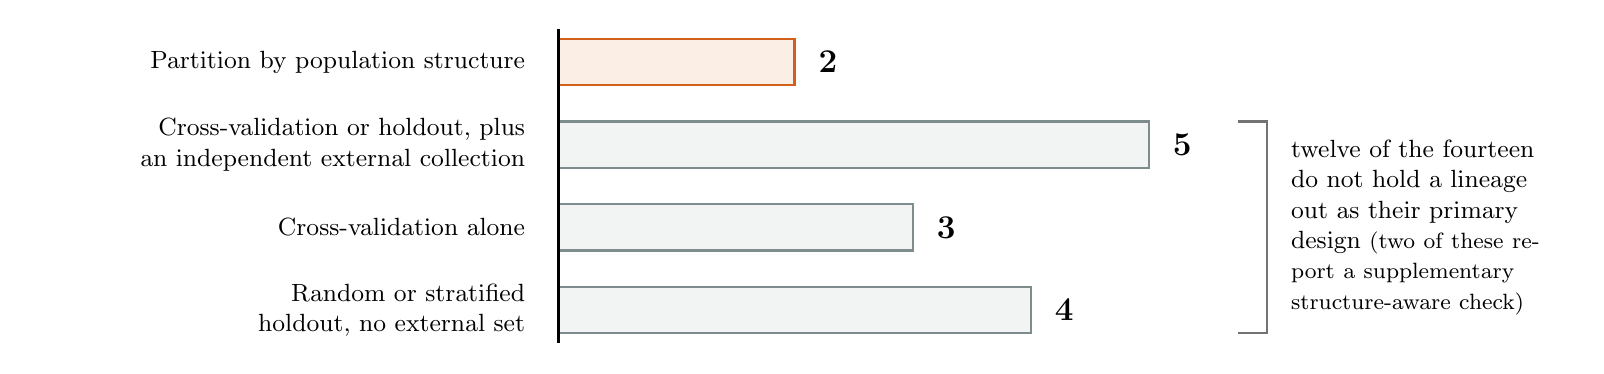
\begin{tikzpicture}[x=1.5cm, y=1.05cm]

% ---- one row per evaluation design: y / count / fill / edge / label ----
% One series, so one colour. Only the row the caption singles out is
% highlighted; the other three are neutral.
\foreach \y/\n/\f/\e/\lab in {%
  0/2/redfill/rededge/{Partition by population structure},
  -1/5/grayfill/neutralc/{Cross-validation or holdout, plus an independent external collection},
  -2/3/grayfill/neutralc/{Cross-validation alone},
  -3/4/grayfill/neutralc/{Random or stratified holdout, no external set}}{
    \fill[\f] (0,\y-0.28) rectangle (\n,\y+0.28);
    \draw[\e,line width=0.9pt] (0,\y-0.28) rectangle (\n,\y+0.28);
    % count, just past the end of the bar
    \node[anchor=west,font=\large\bfseries,text=black] at (\n+0.12,\y) {\n};
    % label, right-aligned in its own column so rows never touch
    \node[anchor=east,font=\small,text=black,align=right,text width=6.2cm]
      at (-0.20,\y) {\lab};
}

% ---- baseline ----
\draw[black,line width=0.9pt] (0,0.40) -- (0,-3.40);

% ---- brace marking the twelve that do not hold a lineage out by design ----
\draw[black!55,line width=0.9pt]
  (5.75,-0.72) -- (6.00,-0.72) -- (6.00,-3.28) -- (5.75,-3.28);
\node[anchor=west,font=\small,text=black,align=left,text width=3.5cm]
  at (6.12,-2.00) {twelve of the fourteen do not hold a lineage out as their
  primary design {\footnotesize(two of these report a supplementary
  structure-aware check)}};

\end{tikzpicture}
}
  \caption{How the fourteen predictive studies of Table~\ref{tab:summary} test
  their models.}
  \label{fig:evalsplit_landscape}
  \fignote{Only two partition by population structure as their primary design. The
  remaining twelve report a headline score from a split that never withholds a
  lineage; two of those twelve add a supplementary structure-aware check alongside
  it. Closing that gap is what this work sets out to do.}
\end{figure}

Even after Yu et al., two gaps remain. Their result is reported as an average across five pathogens, so it establishes that a drop exists without saying which antibiotics carry it. And accounting for structure during splitting is not the same as holding a lineage out, because a split can balance lineage composition across partitions and still leave close relatives on both sides, which measures something quite different. Chapter~\ref{ch:results} returns to this distinction, because we built such a split ourselves before realising it could not answer the question we were asking.

\section{Summary of Key Findings}

Four points follow from this body of work. The first is that reported accuracy is already high and classical models are hard to beat: Random Forest and gradient boosting often match or beat far more complex deep architectures, and the same pattern holds on tabular data generally \cite{grinsztajn2022trees, shwartzziv2022tabular}. Convolutional and attention-based models add value when features are well encoded, such as k-mers or gene presence and absence, but they do not consistently outperform a well-tuned classical method. The second point matters most for this research: evaluation is where the field is weakest. Only two of the fourteen predictive studies in Table~\ref{tab:summary} partition by phylogenetic structure as their primary design \cite{Yu2025, Hu2024}, and both report a drop once they do, so most scores in this field were obtained on strains related to the training set. Section~\ref{subsec:evaldesign} sets out why the correction developed in the association-testing literature \cite{saber2020bacgwas, lees2020pyseer} never carried over, and what a genuine lineage holdout requires that a stratified split does not.

The third point is that most high-performing models remain hard to interpret, and that external validation on a genuinely independent collection is often missing. The fourth is less obvious: the architecture literature our design draws on has developed apart from the AMR application literature. Mixture-of-experts gating, stacked generalisation and attention pooling are mature methods, yet how best to combine several genomic views has drawn far less attention here than which single view to use. Together these four points set the direction of the present research. Rather than adding data types or scaling the model up, we work in one well-characterised genomic setting in \textit{E. coli} and ask how much of the predictive signal is genuine mechanism and how much is relatedness. Honest evaluation, interpretability and generalisation are what separate a reported accuracy from a useful one, and they are what Chapters~\ref{ch:method} and~\ref{ch:results} are built to address.

Table~\ref{tab:summary} summarises the existing research, with the evaluation-split column set apart from the modelling detail because it is the property most relevant to the argument above. Two of its sixteen entries are not predictive studies of a strain phenotype: one is a review \cite{Yun2024}, and one classifies genes into resistance categories rather than predicting resistance for an isolate \cite{ArangoArgoty2018}. Both are listed because they are discussed elsewhere in this chapter, but neither is counted among the fourteen whose split designs are tallied above.

{\footnotesize
\setlength{\tabcolsep}{5pt}
\renewcommand{\arraystretch}{1.25}
\begin{longtable}{|>{\raggedright\arraybackslash}p{2.7cm}|>{\raggedright\arraybackslash}p{3.9cm}|>{\raggedright\arraybackslash}p{2.2cm}|>{\raggedright\arraybackslash}p{4.7cm}|}
\caption{Summary of related works on genomic antimicrobial resistance prediction. The evaluation split column records the partitioning scheme as reported by each study.}
\label{tab:summary}\\
\hline
\textbf{Study} & \textbf{Data and method} & \textbf{Evaluation split} & \textbf{Result and limitation} \\
\hline
\endfirsthead
\hline
\textbf{Study} & \textbf{Data and method} & \textbf{Evaluation split} & \textbf{Result and limitation} \\
\hline
\endhead
\hline
\multicolumn{4}{r}{\footnotesize\textit{Continued on the next page}}\\
\endfoot
\hline
\endlastfoot
Moradi\-garavand et al.\ (2018) \cite{moradigaravand2018} & Pan-genome; gradient boosting, RF, LR; 1,936 \textit{E. coli}, 11 compounds & Random, with an ST131 lineage holdout as a supplementary analysis & Gradient boosting best; feature importance recovers \textit{gyrA} and \textit{parC}; the ST131 holdout scores about 0.28 below a size-matched random control \\ \hline
Her and Wu (2018) \cite{her2018pangenome} & Pan-genome; gene-cluster scoring by genetic algorithm + classifier; 59 \textit{E. coli}, 12 drugs & Leave-one-out cross-validation & Accessory genome carried most signal; very small collection; no lineage-aware holdout \\ \hline
Arango-Argoty et al.\ (2018) \cite{ArangoArgoty2018} & Metagenomic reads; DeepARG vs BLAST best-hit; CARD, ARDB, UNIPROT (14,933 ARGs) & Random 70/30, with external sets & Higher precision and recall than best-hit; classifies genes into resistance categories rather than predicting a strain phenotype \\ \hline
Ren et al.\ (2022) \cite{Ren2022} & WGS, one-hot and FCGR; LR, SVM, RF, CNN; Giessen (987) and public (1,509) \textit{E. coli} & Stratified cross-validation with an independent external set & RF best, AUC around 0.96; class imbalance; associated mutations reported for each antibiotic \\ \hline
Jain et al.\ (2025) \cite{jain2025paeruginosa} & k-mers; two-tier ML with explainable AI; \textit{P. aeruginosa} & Stratified 75/25, with an independent 56-genome set & 79\% accuracy, AUROC 0.77; phylogeny used to weight features but not to split \\ \hline
Gao et al.\ (2024) \cite{Gao2024} & k-mers; RF, SVM, XGBoost; 339 \textit{A. baumannii}, 13 antibiotics & Ten-fold stratified shuffle-split cross-\allowbreak validation, with an independent 120-isolate test set & Essential agreement $>$90.9\%, categorical agreement $>$95.3\%, without curated genes \\ \hline
Do et al.\ (2024) \cite{Do2024} & Unitigs; DBGWAS, GATB, XGBoost; \textit{P. aeruginosa} pan-genome & Ten-fold stratified cross-\allowbreak validation, with an independent 414-isolate collection & Novel candidate resistance genes found; AUC falls from above 0.929 in training to about 0.77 on the independent collection \\ \hline
Serajian et al.\ (2024) \cite{serajian2024mtbpp} & 31-mers; MTB++ (LR, RF); \textit{M. tuberculosis}, 13 drugs & Five-fold cross-validation & Database-free prediction; k-mer ranking computationally heavy \\ \hline
Yun et al.\ (2024) \cite{Yun2024} & Review of machine learning for AMR in foodborne pathogens & Not applicable, review & Reports accuracies up to about 99\% from the studies it surveys; small $n$ for some drug and pathogen pairs \\ \hline
Lopez-Cortes et al.\ (2024) \cite{LopezCortes2024} & MALDI-TOF spectra; MSDeepAMR, transfer learning; three species & Stratified 80/20 with ten-fold cross-\allowbreak validation, and cross-site transfer & About 10\% better than conventional ML; strong transfer-learning gains \\ \hline
Hu et al.\ (2024) \cite{Hu2024} & Benchmarking ResFinder, Kover, PhenotypeSeeker; 78 pathogen-antibiotic pairs & \textbf{Random, phylo\-geny-\allowbreak aware and homo\-logy-\allowbreak aware folds} & No single tool best everywhere; scores fall markedly under phylogeny-aware folds \\ \hline
Wang et al.\ (2025) \cite{Wang2025} & SNPs and gene P/A; XGBoost with SHAP; 296 \textit{H. pylori}, 4 antibiotics plus MDR & Random & Consistently strong AUC; SHAP flagged 23S rRNA mutation; no external validation \\ \hline
Orcales et al.\ (2024) \cite{Orcales2024} & Genomic; LR, RF, XGBoost, NN; 1,936 \textit{E. coli} & Cross-validation, with an MLST-blocked option & XGBoost most reliable; warns about overfitting and feature misreading \\ \hline
Paredes-Gutierrez et al.\ (2025) \cite{ParedesGutierrez2025} & Mutations; XGBoost, LightGBM, ANN; 847 \textit{M. tuberculosis} & Random 677/170, with ten-fold cross-\allowbreak validation inside training & Accuracy about 97\% for XGBoost and 95\% for LightGBM; intergenic mutations important; ANN worst \\ \hline
Siddiqui and Tarannum (2026) \cite{siddiqui2025amrensemble} & Motifs + pan-genome; 1D CNN + XGBoost ensemble; Giessen (809) \textit{E. coli}, 4 antibiotics & Stratified 80/20 holdout & MCC 0.926 for CIP, macro F1 0.691 for GEN; attributions concentrate on \textit{fusA} and \textit{parC}; assumes positional order is informative \\ \hline
Yu et al.\ (2025) \cite{Yu2025} & Genomic; LightGBM; over 24,000 genomes, 5 pathogens & \textbf{Phylogeny-\allowbreak aware} & Accuracy drops when phylogenetic structure is ignored; more data does not fix it \\ \hline
\end{longtable}}

\subsection{Comparative Analysis}

Table~\ref{tab:summary} records what each study did; Table~\ref{tab:comparison} sets
the closest six side by side on the points that matter here. Those six work on the
same organism, the same collections, or the same question of population structure.
The remaining entries differ in organism, so a column-by-column comparison with them
would not be informative.

\begin{table}[H]
\centering
\caption{The proposed approach against the six most closely related studies. Each
cell records only what the study reports; N/A means the study does not
report that property, not that it was attempted and failed.}
\label{tab:comparison}
\renewcommand{\arraystretch}{1.3}
\setlength{\tabcolsep}{3.5pt}
\footnotesize
\begin{tabular}{|>{\raggedright\arraybackslash}p{2.1cm}|>{\raggedright\arraybackslash}p{2.0cm}|>{\raggedright\arraybackslash}p{2.4cm}|>{\raggedright\arraybackslash}p{1.8cm}|>{\centering\arraybackslash}p{1.5cm}|>{\raggedright\arraybackslash}p{1.7cm}|>{\raggedright\arraybackslash}p{1.6cm}|}
\hline
\textbf{Study} & \textbf{Organism and scale} & \textbf{Genomic views combined} & \textbf{Evalua\-tion split} & \textbf{Preval.\ correction} & \textbf{Interpre\-tation} & \textbf{External collection} \\
\hline
Moradi\-garavand et al.\ (2018) \cite{moradigaravand2018} & \textit{E. coli} \newline 1,936 strains \newline 11 drugs & Pan-genome; population structure as an input feature & Random; ST131 holdout in a supple\-ment & \na & Feature import\-ance (\textit{gyrA}, \textit{parC}) & \na \\ \hline
Ren et al.\ (2022) \cite{Ren2022} & \textit{E. coli} \newline 987 + 1,509 strains \newline 4 drugs & One-hot and FCGR encodings of WGS & 5$\times$5-fold stratified cross-\allowbreak validation & \na & Associated mutations reported & Trained on one collection, tested on another \\ \hline
Orcales et al.\ (2024) \cite{Orcales2024} & \textit{E. coli} \newline 1,936 strains & Single genomic view & Cross-validation; MLST-blocked option & \na & \na & \na \\ \hline
Wang et al.\ (2025) \cite{Wang2025} & \textit{H. pylori} \newline 296 strains \newline 4 drugs plus MDR & SNPs and gene presence/absence & Random & \na & SHAP & None reported \\ \hline
Siddiqui and Tarannum (2026) \cite{siddiqui2025amrensemble} & \textit{E. coli} (Giessen) \newline 809 strains \newline 4 drugs & SNP motifs and pan-genome, ensembled & Stratified 80/20 & \na & Attribu\-tion (\textit{fusA}, \textit{parC}) & \na \\ \hline
Yu et al.\ (2025) \cite{Yu2025} & 5 pathogens \newline over 24,000 strains & Single genomic view & \textbf{Phylo\-geny-\allowbreak aware} & \na & \na & \na \\
\hline\hline
\textbf{This work} & \textbf{\textit{E. coli} (Arcadia)} \newline \textbf{6,962 strains} \newline \textbf{7 drugs} & \textbf{SNP motifs, pan-genome and cross-antibiotic structure, gated and stacked} & \textbf{Random and MLST lineage holdout} & \textbf{Yes} & \textbf{SHAP and attention weights} & \textbf{Giessen, retrained} \\ \hline
\end{tabular}
\end{table}

\vspace{1em}

If we only take a look at the scale and views columns, the proposed work is not
that much different from the other studies. The collection is larger than most single-organism studies here but
smaller than the multi-pathogen one, and combining several genomic views is a
difference of degree rather than of kind:
Ren et al. and Siddiqui and Tarannum both combine encodings, and the gain we
measure from our own neural design over a well-tuned classical learner is small
enough to sit inside its confidence interval, which is consistent with what the
tabular-data literature reports \cite{grinsztajn2022trees}. A claim of novelty
resting on architecture width alone would therefore be weak, and we do not make
one. What the architecture does contribute is narrower and can be stated
precisely: gated attention pooling, used unchanged, collapses to a single gene
ranking shared by every strain, because the quantity it scores for a
present gene is the gene embedding itself. Conditioning that score on the strain's
own gene content removes the degeneracy, and Chapter~\ref{ch:results} measures what
it is worth.

The separation is in the last four columns. Of the fourteen predictive studies in
Table~\ref{tab:summary} two split with phylogeny in mind, and none
reports the correction that such a split makes necessary. A lineage holdout does
not only remove relatedness from the test set; it also changes how many strains in
it are resistant, and PR-AUC is read against a no-skill baseline equal to that
share. A drop measured without correcting for it therefore mixes a real loss of
generalisation with an artefact of the metric, and the two are not separable after
the fact. Feature selection needs the same care: unless it is refitted on each split's own
training partition, the selection itself carries test information across the divide. This is why
the contribution we defend is a protocol rather than a score: the model exists to
make the measurement worth trusting, and the measurement is what transfers to
other organisms in which population structure and resistance travel together.
External validation and interpretation follow the same rationale, since an attribution
that restores an established mechanism and a model retrained on an independent
collection are both checks on whether the number means what it appears to mean.


\chapter{Requirements, Impacts and Constraints}
\label{ch:req}

Four points had to be clear before the development of the model started: what the system was
supposed to do, how its success would be measured, which limits it must obey, and what
resources it had. Setting these points out early ensured that the later assessment was fairer.
As an illustration, Chapter~\ref{ch:results} is able to show clearly that the system could not
comply with the clinical error limits for all seven antibiotics, because those limits had been
defined in advance. The broader impacts of the work, such as societal and environmental impact,
ethical concerns, standards, project planning, risks, and cost, are also discussed in this
chapter.

\section{Final Specifications and Requirements}
\label{sec:specs}

The requirements were based on the literature analysed in Chapter~\ref{ch:lit}~\cite{Kim2022,
Sakagianni2023}, the available data, and supervisor reviews after every stage. No clinician,
clinical microbiologist or laboratory technician was consulted. This represents an important
limitation, as the requirements were not verified directly with those who would use such a
system.

\subsection{Functional Requirements}

The system has an impact on clinicians, microbiologists, health services, researchers, and
patients. However, the requirements relate mainly to clinicians and patients, because they are
the ones who bear the cost of an incorrect prediction. Even a high average score may conceal a
severe case in which a resistant isolate has been reported as susceptible. Thus, the error
rates for every drug are recorded and the very major errors are measured
separately~\cite{Kim2022, Hu2024, who_amr_2019, Yu2025}. The ten requirements listed in
Table~\ref{tab:funcreq} were established prior to development. FR9 was the only one revised
later, for the reason given below.

{\small\setlength{\tabcolsep}{5pt}
\begin{longtable}{|l|>{\raggedright\arraybackslash}p{3.0cm}|>{\raggedright\arraybackslash}p{9.8cm}|}
\caption{Functional requirements of the proposed system.}
\label{tab:funcreq}\\
\hline
\textbf{ID} & \textbf{Requirement} & \textbf{What it means} \\
\hline
\endfirsthead
\hline
\textbf{ID} & \textbf{Requirement} & \textbf{What it means} \\
\hline
\endhead
\hline
\multicolumn{3}{r}{\footnotesize\textit{Continued on the next page}}\\
\endfoot
\hline
\endlastfoot
FR1 & Genomic input &
The system must accept whole genome information for \textit{Escherichia coli}. It must build
SNP features and gene presence or absence features automatically, without a bioinformatician
editing them by hand. \\
\hline
FR2 & More than one lens on the genome &
The system must describe each isolate's genome through more than one lens, so that
variant-level and gene-level information are both available to the model. \\
\hline
FR3 & Prediction for several drugs &
The system must predict resistant or susceptible for seven antibiotics covering five drug
classes. The penicillins are ampicillin (AMP) and amoxicillin with clavulanic acid (AMC); the
cephalosporins are cefotaxime (CTX) and ceftazidime (CAZ). Ciprofloxacin (CIP) is a
fluoroquinolone, gentamicin (GEN) an aminoglycoside, and trimethoprim with sulfamethoxazole
(SXT) a folate pathway inhibitor. \\
\hline
FR4 & Score instead of a plain label &
The system must return a score for each drug rather than a yes or no answer, so that the user
decides where the cut-off falls. \\
\hline
FR5 & Separate cut-off per drug &
The system must allow a different decision threshold for each antibiotic, because the cost of
a given error is not equal across drugs. \\
\hline
FR6 & Handling of missing labels &
The system must be trained with isolates tested against only some of the seven drugs, since
natural collections only test a small proportion of isolates for each drug. A boolean mask is
included with the label matrix, so
an untested drug is not read as a susceptible result nor is it allowed to contribute a
gradient. \\
\hline
FR7 & Interpretability output &
The system must produce interpretability output for every prediction. That output names the
genes which received the highest attention weights and the weight the gate placed on each
lens. \\
\hline
FR8 & Statistical reporting &
The system must produce bootstrap confidence intervals and significance tests against
competing models as part of its ordinary output. \\
\hline
FR9 & More than one kind of split &
The system must be evaluated under three splits: a random split, a phylogroup-stratified split
matching lineage composition across partitions, and a lineage holdout in which no sequence
type appears in more than one partition. The effect of relatedness on the reported score is
then measured at more than one level of detail. \\
\hline
FR10 & External validation &
The system must be evaluated on a different isolate collection that was used neither for
training nor for model selection. \\
\end{longtable}}

FR8, FR9 and FR10 were added from the beginning, since evaluation is core to this research. The
key question is not only whether resistance can be predicted, but also whether the model learns
resistance biology or population structure~\cite{Yu2025}. FR9 originally requested a random
split and a phylogeny-aware split. The initial phylogroup-stratified split resulted in balanced
broad lineages but no separation of close relatives. Thus, FR9 was amended to require a
sequence-type lineage holdout. This change is explained as Risk R1 in Section~\ref{sec:risk}.

\subsection{Non-Functional Requirements}

The performance targets were set prior to the final evaluation. They were fixed as minimum
acceptable levels and not as hoped-for results, to minimise the risk of adjusting the model
until it matched the test set. Table~\ref{tab:nonfuncreq} shows the non-functional requirements
that were identified and how each of them was verified.

{\small\setlength{\tabcolsep}{5pt}
\begin{longtable}{|l|>{\raggedright\arraybackslash}p{2.7cm}|>{\raggedright\arraybackslash}p{6.0cm}|>{\raggedright\arraybackslash}p{3.6cm}|}
\caption{Non-functional requirements and how each was verified.}
\label{tab:nonfuncreq}\\
\hline
\textbf{ID} & \textbf{Requirement} & \textbf{Target} & \textbf{How it was checked} \\
\hline
\endfirsthead
\hline
\textbf{ID} & \textbf{Requirement} & \textbf{Target} & \textbf{How it was checked} \\
\hline
\endhead
\hline
\multicolumn{4}{r}{\footnotesize\textit{Continued on the next page}}\\
\endfoot
\hline
\endlastfoot
NFR1 & Predictive quality &
Mean precision-recall AUC must reach at least 0.80 across the seven drugs on the random split.
Precision-recall AUC replaces accuracy because the classes are
imbalanced~\cite{saito2015, davis2006}. The target applies to the random split alone, since
that is the split carrying the baseline comparison; lineage-holdout results are reported
separately and are not measured against it. &
Measured on a held-out test set. \\
\hline
NFR2 & Statistical rigour &
Headline comparisons must carry a bootstrap confidence interval, and headline results must be
reported on all three splits. &
Bootstrap resampling, 1{,}000 rounds. \\
\hline
NFR3 & Reproducibility &
A fixed seed must reproduce output exactly, with every experiment setting under version control
and every training run logged. &
Reported numbers re-created from saved settings. \\
\hline
NFR4 & Training cost &
Full training must complete on one consumer GPU in hours rather than days. &
Fit times recorded for all experiments. \\
\hline
NFR5 & Inference speed &
Prediction for all seven drugs must take under one second per isolate once the genome is
assembled. &
Timed on the target workstation. \\
\hline
NFR6 & Memory &
The complete gene presence and absence matrix, before any gene filtering is applied, must fit
in the working memory of a single workstation. Its dimensions are the isolate and gene counts
given in Table~\ref{tab:constraints}. &
Peak memory monitored while the unfiltered matrix was built. \\
\hline
NFR7 & Interpretability &
Attention and gate weights must be available for every prediction and rankable by gene for each
drug. &
Per-drug gene ranking tables were produced. \\
\hline
NFR8 & Honest reporting of failure &
Clinical error limits that are not met must be reported as unmet, not hidden by selecting a
convenient threshold. &
Clinical error rates reported at a fixed threshold. \\
\hline
NFR9 & Maintainability &
Stages must be separable, so that changing one stage does not force the whole pipeline to be
re-run. &
Each stage writes its output before the next begins. \\
\hline
NFR10 & Improvement over the baseline &
Mean precision-recall AUC must exceed 0.803, the project's first classical baseline. That
baseline is an XGBoost model on 1{,}024 principal component features, built before the
gene-level baseline of Stage 2. NFR1 fixes an absolute floor; this requirement fixes a
relative one, against the project's own starting point. &
Compared drug by drug against the recorded baseline results. \\
\hline
NFR11 & Clinical error limits &
Very major and major error rates must both fall inside the CLSI limit for every drug at the
chosen operating point. &
Checked per drug and saved in the clinical metrics output. \\
\end{longtable}}

The mean precision-recall AUC of the final system was 0.849. This beat NFR1 by 0.049 and the
original baseline in NFR10 by 0.045. That baseline was not even: it ranged from 0.655 for
gentamicin to 0.948 for ciprofloxacin. The mean, however, masks significant variations between
the drugs. The improvement varied from 0.125 for trimethoprim-sulfamethoxazole to just 0.0005
for amoxicillin-clavulanate. Both models round to 0.748 for the latter. The majority of the
gain was also observed prior to the inclusion of the neural components. The classical model
improved from 0.803 to 0.830 when replacing principal components with gene-level features. The
best single classical learner eventually reached 0.840, leaving the final system only 0.009
ahead. This stronger baseline was not taken into account when defining NFR1 and NFR10.

\subsection{Constraints}

There were four conditions in the data and project setting that were fixed for the design.
These were not modelling choices; they were restrictions imposed on any prospective design.

{\small\setlength{\tabcolsep}{5pt}
\begin{longtable}{|>{\raggedright\arraybackslash}p{2.8cm}|>{\raggedright\arraybackslash}p{5.0cm}|>{\raggedright\arraybackslash}p{6.1cm}|}
\caption{Design constraints and their effect on the system.}
\label{tab:constraints}\\
\hline
\textbf{Constraint} & \textbf{Description} & \textbf{Effect on the design} \\
\hline
\endfirsthead
\hline
\textbf{Constraint} & \textbf{Description} & \textbf{Effect on the design} \\
\hline
\endhead
\hline
\multicolumn{3}{r}{\footnotesize\textit{Continued on the next page}}\\
\endfoot
\hline
\endlastfoot
Sample size & 6{,}962 labelled isolates in 8 phylogroups, a large number for genomic resistance
prediction and a small one for deep learning~\cite{goodfellow2016dl} &
Large neural models were ruled out. The design had to pair a small neural component with
classical learners rather than scale up. \\
\hline
Class imbalance & Some drugs, gentamicin above all, carry far fewer resistant than susceptible
isolates &
Accuracy carries no information here. Precision-recall AUC and MCC were used
instead~\cite{saito2015}, and confidence intervals became mandatory. \\
\hline
Number of features & 535{,}439 candidate SNP features and a pan-genome catalogue of 32{,}441
genes against only 6{,}962 isolates &
Heavy feature reduction was required before modelling, down to 5{,}000 genes, because every
extra free parameter is capacity to fit noise. \\
\hline
No laboratory access & The project is computational throughout, with no means of checking a
prediction by culture &
Every claim is a claim about data, not about biology confirmed at the bench. Interpretability
findings are hypotheses to be tested, not proven mechanisms. \\
\end{longtable}}

The greatest constraint is the absence of laboratory facilities. When the model gives high
importance to a gene, it only reflects that the model used that feature. It cannot demonstrate
that the gene is responsible for resistance. Laboratory experiments beyond the scope of this
research would be needed to confirm such a mechanism.

\subsection{Delivered System Specification}

These requirements led to TriLens-MoE-Stack. Three neural lenses model the genome in three
different ways and are then combined via a mixture-of-experts gate for each isolate and drug.
Their outputs are used with five classical base learners, followed by a separate logistic
regression meta-learner for each drug. Chapter~\ref{ch:method} details the complete
architecture and training process. All values reported here are found in the saved experiment
configurations.

The data are based on the Arcadia \textit{E. coli} collection~\cite{arcadia2024,
morin2024ecoli}. Table~\ref{tab:constraints} lists its size and the number of features in it,
and the rules of filtering are provided in Section~\ref{sec:data}. Each of the seven drugs,
AMP, CIP, AMC, SXT, GEN, CTX, and CAZ, is predicted in the three settings defined in
Section~\ref{subsec:splits}: a random split, a phylogroup-stratified split, and a sequence-type
lineage holdout. The external test is not a held-out test of this model. The two collections
have no features in common. Thus, only the classical stacking part was rebuilt on the Giessen
collection, with the four shared drugs and without the neural lenses.

\subsection{Compliance Against Requirements}

Figure~\ref{fig:requirements_status} summarises the outcome for all twenty-one requirements at
a glance, and the paragraphs below give the reasons.

\begin{figure}[H]
\centering
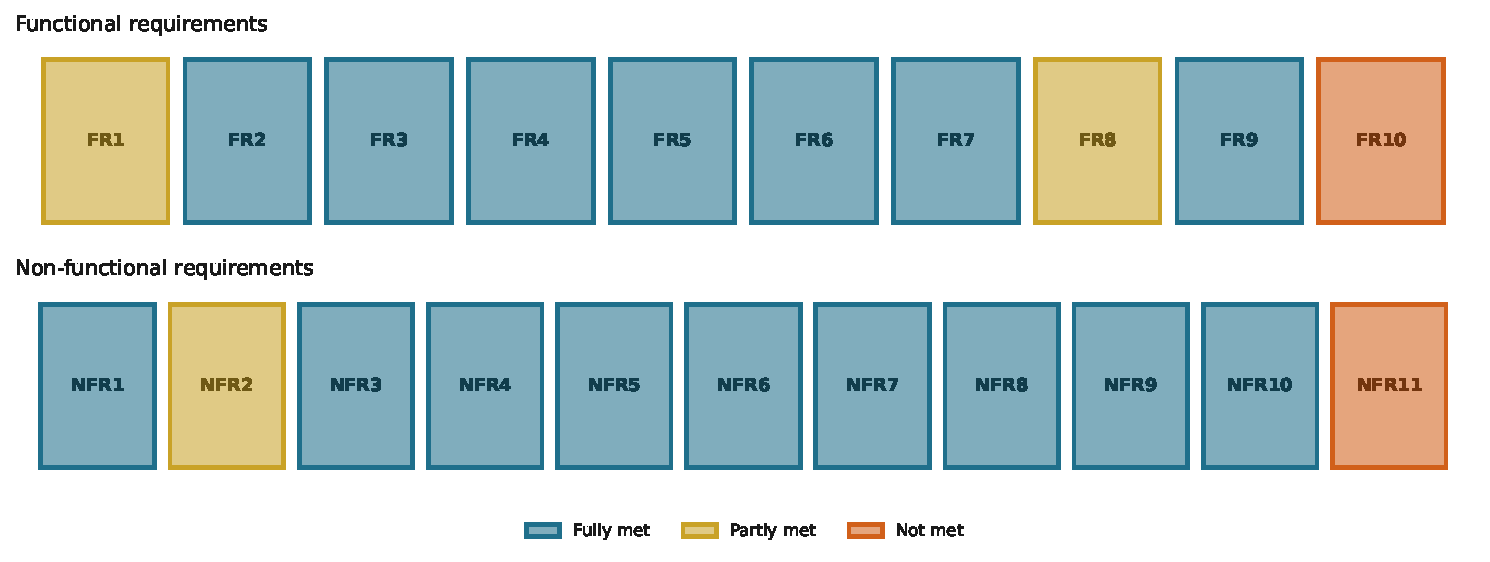
\includegraphics[width=\textwidth]{fig_requirements_status.pdf}
\caption{Compliance against every requirement fixed in advance.}
\label{fig:requirements_status}
\fignote{Of the ten functional requirements seven were fully met, two partly met and
one not met; of the eleven non-functional requirements nine were fully met, one
partly met and one not met. FR10 and NFR11 are the two that were not met.}
\end{figure}

Ten functional requirements were defined. Seven of them were fully met, two were only partly
met, and one was not met. FR1 was partially fulfilled, as features were generated from
existing variant calls in Arcadia, not directly from raw sequencing reads. FR8 was also
partially fulfilled, since baseline differences were evaluated using bootstrap intervals rather
than formal tests of significance. FR10 was not achieved, as the classical stack was retrained
on the Giessen collection rather than using a single fixed Arcadia-trained model.

Eleven non-functional requirements were defined. Nine of them were fully met, one was only
partly met, and one was not met. The mean score was 0.849, which is higher than the target of
0.80, so NFR1 was
met. Gentamicin (0.704) and amoxicillin-clavulanate (0.748), however, were still below 0.80
individually. NFR10 was met on average, and every drug scored at or above its own baseline,
though for amoxicillin-clavulanate the margin was only 0.0005. NFR2 was only partially
achieved, since confidence intervals were provided for the key comparisons but not for every
table in Chapter~\ref{ch:results}.

NFR11 was not met. The CLSI acceptance limits are 0.03 for major and very major errors.
Ciprofloxacin (0.015), gentamicin (0.023), and cefotaxime (0.026) fulfilled the major error
limit. However, no drug met the very major error limit, which ranged from 0.086 for
ciprofloxacin to 0.436 for gentamicin. Thus, no drug met both thresholds. Full results are
presented in Table~\ref{tab:clinical} in Chapter~\ref{ch:results}, with effects on responsible
use highlighted in Chapter~\ref{ch:conclusion}.

\section{Societal Impact}
\label{sec:societal}

A system that fails to catch resistance in every drug cannot be evaluated on its scores alone.
Its value is determined by what a clinician would do with it and by whom it would help.
Effective antibiotics are critical to many modern medical applications, such as surgery,
caesarean deliveries, chemotherapy, organ transplantation and care of premature
infants~\cite{who_amr_2019}. Antibiotic resistance reduces this protection, especially in
settings where few alternative drugs are available. There are few new classes of antibiotics,
so the existing ones must be used more carefully. Early prediction of resistance can help with
this, by making clinicians aware of the drugs that are unlikely to be effective.

Typically, culture-based susceptibility testing requires one or two days, since it involves
growing the organism and testing it against multiple drugs~\cite{Kim2022, Ren2022}. Treatment
can begin even before the result is available. A clinician can opt to use a drug that fails, or
resort to a broad-spectrum drug which is safer. The latter option can benefit the current
patient, yet it adds to the antibiotic pressure. The goal of good stewardship is to select the
narrowest effective drug for the shortest possible time~\cite{who_amr_2019}. An early
prediction can help with that decision while the laboratory result is still pending.

The situation is even more serious where laboratory testing is limited. In Bangladesh and other
South Asian countries, full susceptibility testing is mainly accessible in big cities, and
antibiotics can be purchased over the counter~\cite{who_amr_2019, Branda2024}. Treatment can be
initiated prior to the collection of a sample, and antibiotic courses can be discontinued when
the symptoms subside. These problems cannot be solved by a prediction system alone. Prescribing,
laboratory access, and clinical practice would also need to change to achieve better outcomes.
This work is intended to offer information; it is not a complete behavioural or health-system
solution.

There are practical benefits of a computational system. It does not require reagents, kits, or
cold storage, and a trained model can be replicated or retrained with local data. However,
sequencing is still required. Additionally, many resistant isolates are missed, including 0.436
for gentamicin and 0.394 for amoxicillin-clavulanate. So it should aid laboratory testing, not
replace it. At present, the system functions better as a regional resistance monitoring tool
than in making treatment decisions for individual patients.

Further constraining use of the system is the error pattern. Four of the drugs had major errors
below 0.04, but only three fell within the CLSI limit of 0.03. Very major errors were between
0.086 and 0.436, and were above the limit for every drug. Thus, the model can be useful for
identifying drugs that should be avoided until culture results are received. A drug should not
be prescribed only because the model predicts that it will be susceptible.

There is also an equity issue with the generalisation results. Performance was lower under the
sequence-type lineage holdout, when close relatives were excluded from training, and the extent
of the decrease was drug-dependent. This indicates that some of the predictive power of the
model comes from population structure instead of resistance biology~\cite{Yu2025}. Europe and
North America are also dominant in public genome collections~\cite{Yu2025}. Consequently,
models can perform poorly on underserved populations that already have limited access to
diagnostics. For this reason, all three data splits are reported and their differences are
regarded as an important result.

\section{Environmental Impact}
\label{sec:environment}

The argument presented above hinges on prescribing fewer and narrower spectrum antibiotics.
This would also be the most substantial environmental gain from this work, but it is by no
means the only quantity involved. Computation is a cost in itself, and it is only that side
which can be estimated from this project.

All experiments ran on one consumer GPU workstation. No cloud or cluster resources were required
and mixed precision was employed throughout. The longest full run was approximately 140 minutes
in duration. Across all experiments, the approximate energy consumption was 20--30 kWh. This is
just an estimated figure as no power meter was used. While low energy use was not a formal
goal, the final designs were both accurate and relatively cheap to run.

The potential for an environmental benefit is reduced antibiotic use. Antibiotic residues end
up in water and soil, where they continue to select for resistance~\cite{Liu2024}. This
pressure could be lowered with more targeted treatment. Some laboratory materials, such as
plates and media, may also be saved by computational prediction. Neither of these effects was
measured, however, and confirmatory culture is still necessary because of the current error
rates. The trained model is inexpensive to replicate, and will require retraining in the
future, as circulating lineages evolve.

\section{Ethical Issues}
\label{sec:ethics}

Counting energy and materials is easy, whereas it is more difficult to count the duties imposed
by a clinical system. They are not removed by writing correct code. This project was
guided by six duties: privacy, harm, equity, research integrity, benefit sharing, and dual use.

This is not a set of human genomes, but rather bacterial genomes. All data came from an open
community repository~\cite{morin2024ecoli, york2025amr}. No patient identifiers, clinical notes
or treatment records were involved. The pipeline only reads genome and sample identifiers,
phylogroups and antibiotic labels. No isolate was associated with an institution or person.

The main risk is over-reliance on the prediction. A very major error may result in a
non-functional drug, and none of the drugs passed the required limit. The system is also
described throughout as unvalidated for clinical use, and intended only as decision support alongside
laboratory testing, as mentioned in Section~\ref{sec:societal}.

The model is more accurate if there are related strains in the training set, and this is not
uniformly distributed across populations~\cite{Yu2025}. For this reason, the performance
difference between the three evaluation splits is made transparent.

Often, resistance prediction models appear good, but are not effective when careful testing is
conducted~\cite{Hu2024}. Three practices were used to avoid this. First, not only the direction
of each improvement is reported but also the size. This contains a negative finding: a more
complex neural meta-learner was worse than the simple one. The small margin mentioned in risk
R8 in Section~\ref{sec:risk} is also reported publicly. Second, a malfunction in the
resistance-gene keyword filter was discovered during the project, fixed, and the analysis
re-run. It is listed as R5 in Table~\ref{tab:risks}. Third, before the final comparisons, all
thresholds and protocols were set. Seeds, configuration files and run logs were saved, and thus
any reported number can be reproduced.

It is a more difficult question to ask who benefits than it is to ask who is harmed. The data
imbalance described in Section~\ref{sec:societal} indicates that the population with the
greatest impact from resistance is not the most well represented in this data set. This gap is
not due to a modelling decision in this project, but rather is due to the data available.
However, some measures were taken to ensure that it did not become worse. All libraries and
genomes used are open. The pipeline runs on a single consumer graphics card, and not on cluster
time. Errors are also reported per drug, so another group working on another local lineage can
see exactly what it would inherit.

The dual-use risk is low. Predicting resistance is not a means to produce or transfer
resistance. The algorithms and data are all publicly available, but the work also depends on
access to the organism and sequencing capacity.

\section{Standards}
\label{sec:standards}

Many of those responsibilities rely on being comprehended. If someone reading an error rate for
each drug cannot tell which errors matter, it helps no one, so this work borrowed its
vocabulary rather than inventing one. Although the system is not clinically validated, the
errors it identifies are characterised in terms already used by diagnostic practice. The
standards and codes of practice applied to the work are shown in Table~\ref{tab:standards}.

{\small\setlength{\tabcolsep}{5pt}
\begin{longtable}{|>{\raggedright\arraybackslash}p{3.3cm}|>{\raggedright\arraybackslash}p{3.2cm}|>{\raggedright\arraybackslash}p{7.4cm}|}
\caption{Standards and codes of practice applied to the work.}
\label{tab:standards}\\
\hline
\textbf{Standard or practice} & \textbf{Area} & \textbf{How we used it} \\
\hline
\endfirsthead
\hline
\textbf{Standard or practice} & \textbf{Area} & \textbf{How we used it} \\
\hline
\endhead
\hline
\multicolumn{3}{r}{\footnotesize\textit{Continued on the next page}}\\
\endfoot
\hline
\endlastfoot
CLSI susceptibility reporting & Clinical microbiology &
Errors are reported as per the standard definitions: very major error (VME), major error (ME)
and categorical agreement, following the clinical evaluation practice described for machine
learning based resistance prediction~\cite{Kim2022, Hu2024}. The result for each drug is
compared against the limits and reported. \\
\hline
Reproducible-research practice & Configuration, seeding and logging &
Hydra configuration files are versioned and kept separate from the code, and the seed is set to
42 for splitting, initialisation, folds and bootstrap. All training runs, including discarded
ones, are recorded externally, so the settings behind any reported number can be recovered
exactly. \\
\hline
Open source licensing & Software &
All libraries used by the pipeline are openly licensed, so the pipeline can be shared and
reused freely. \\
\hline
University academic integrity policy & Research conduct &
All sources cited, all negative results reported, no selection of favourable runs. \\
\end{longtable}}

CLSI reporting is especially critical since common machine learning metrics do not provide
direct indications of patient-safety risk. Accuracy, ROC-AUC, and F1 are commonly
reported~\cite{Hu2024}, whereas precision-recall AUC is more well-suited to imbalanced
classes~\cite{saito2015, davis2006}. But these measurements are primarily used to compare
models. Very major errors (VME), major errors (ME) and categorical agreement link the results
to clinical safety. The data were published for re-use~\cite{arcadia2024} and the software stack is open
source, meaning that the pipeline can be reimplemented and expanded.

These standards were followed voluntarily in this research. Much more would be needed for
clinical deployment. Programs that have an impact on diagnosis or treatment are typically
considered a medical device, and machine learning further introduces new challenges since
performance is dictated by the training data~\cite{Duggirala2025}. Before patient use, formal
clinical validation, documented claims and regulatory approval would be required. None of these
steps have been performed.

\section{Project Management Plan}
\label{sec:planning}

The practice of reproducible-research, as shown in Table~\ref{tab:standards}, was incorporated
in the schedule and not just tacked on at the end. The results of each stage of the project
were stored prior to the next stage. This saved on the re-running of unnecessary results, and
established a clear connection between each result reported and its origin file. It also helped
achieve the reproducibility goal in NFR3. Project stages, deliverables and outcomes are shown
in Table~\ref{tab:phases}.

{\small\setlength{\tabcolsep}{5pt}
\begin{longtable}{|l|>{\raggedright\arraybackslash}p{3.0cm}|>{\raggedright\arraybackslash}p{9.6cm}|}
\caption{Project stages, deliverables and outcomes.}
\label{tab:phases}\\
\hline
\textbf{Stage} & \textbf{Focus} & \textbf{Deliverable and outcome} \\
\hline
\endfirsthead
\hline
\textbf{Stage} & \textbf{Focus} & \textbf{Deliverable and outcome} \\
\hline
\endhead
\hline
\multicolumn{3}{r}{\footnotesize\textit{Continued on the next page}}\\
\endfoot
\hline
\endlastfoot
1 & Data collection and preparation &
Genomes assembled, variants called, susceptibility labels extracted for seven drugs, and
training, validation and test splits defined and frozen. \\
\hline
1.5 & Feature reduction &
Chi-squared pre-filtering and XGBoost importance ranking to trim the feature space to
5{,}000 genes, with the number of genes retained at each step recorded for auditing. \\
\hline
2 & Classical baseline &
Gene-aggregated gradient boosting achieved approximately 0.830 mean precision-recall AUC,
establishing the baseline any proposed system had to exceed. \\
\hline
3 & Neural modules &
The mixture-of-experts and attention-based gene models were constructed. The result was
negative: no neural model alone performed better than the classical baseline. \\
\hline
4 & Stacking &
Several stacking designs were created, with classical and neural base learners communicating
via a meta-learner. It was found that interaction, not any one model, was the direction to
take. \\
\hline
5 & Final model and ablation &
The architecture was completed and a step-wise ablation was carried out to dissect the
contributions of fusion, the meta-learner and the decision threshold. \\
\hline
6 & Validation studies &
Locality testing, interpretability analysis, phylogroup-stratified evaluation and transfer to
an external collection generated the generalisation results. \\
\hline
7 & Statistical analysis &
Bootstrap confidence intervals, prevalence-matched resampling, threshold-tuning checks and
clinical error rates were calculated. \\
\hline
8 & Documentation &
Research report, figures, defence materials and the journal version of the work were prepared. \\
\end{longtable}}

The component stages of the model used in the ablation study in Chapter~\ref{ch:results} are
different from the stage numbers above, which are project phases.

Two consumer graphics cards were used in the work. An NVIDIA RTX 4080 SUPER was the main
device, and an RTX 4070 Ti was used for development, so one hardware failure could not stop the
project. The software was an open-source standard Python stack. The neural lenses and the gate
were implemented with the help of PyTorch and Lightning. XGBoost, LightGBM, and scikit-learn
were used for the classical base learners and the
meta-learner~\cite{chen2016xgboost, ke2017lightgbm, breiman2001rf}, and SHAP was used for
attribution. All the experiment configurations and training runs were recorded by Hydra and
Weights and Biases. Precise package versions are stored in the project environment file instead
of in this list.

There was no dedicated budget and the timeline relied on the time and computing capabilities of
a single workstation, as Section~\ref{sec:economic} outlines. The supervisor assessed the
progress following each stage and these assessments informed the subsequent stage. One review
switched the principal components for gene-level features, which resulted in a better baseline
of 0.830, while also being more interpretable. Another review decided to reject a neural
meta-learner because it gave worse results than logistic regression. All stages yielded a
usable product, which meant that if any later stages had not been included, the project could
have still been finished.

\section{Risk Management}
\label{sec:risk}

The main risks were established at the beginning of the project and re-evaluated at the end of
each project stage. All the risks in Table~\ref{tab:risks} have happened or were so severe as
to necessitate a clear control.

{\small\setlength{\tabcolsep}{5pt}
\begin{longtable}{|l|>{\raggedright\arraybackslash}p{4.3cm}|>{\raggedright\arraybackslash}p{1.5cm}|>{\raggedright\arraybackslash}p{1.4cm}|>{\raggedright\arraybackslash}p{5.0cm}|}
\caption{Project risk register with severity, occurrence and mitigation.}
\label{tab:risks}\\
\hline
\textbf{ID} & \textbf{Risk} & \textbf{Severity} & \textbf{Occurred} & \textbf{What we did} \\
\hline
\endfirsthead
\hline
\textbf{ID} & \textbf{Risk} & \textbf{Severity} & \textbf{Occurred} & \textbf{What we did} \\
\hline
\endhead
\hline
\multicolumn{5}{r}{\footnotesize\textit{Continued on the next page}}\\
\endfoot
\hline
\endlastfoot
R1 & Results are too good because related isolates appear in both the training and the test
set &
High & Yes &
Constructed a phylogroup-stratified split first, which failed to answer the question, followed
by a real sequence-type lineage holdout~\cite{Yu2025}. Rather than quietly patching the defect,
we report the correction as one of the principal findings. \\
\hline
R2 & Overfitting on a small and imbalanced dataset & High & Partly &
Early stopping with patience 8, regularised base learners, out-of-fold meta-learner inputs and
bootstrap confidence intervals on every score. \\
\hline
R3 & Results are valid only for the collection the model was trained on & High & Partly &
Rebuilt the classical stack independently on a second collection and measured the performance
retained by the method. \\
\hline
R4 & Insufficient resistant isolates for some drugs, making estimates unstable &
Medium & Yes &
Instead of accuracy, reported precision-recall AUC and MCC with confidence intervals, so that
the weaker drugs show clearly that they are less certain. \\
\hline
R5 & Interpretability analysis errors leading to incorrect biological claims & Medium & Yes &
A loose substring match in the resistance-gene keyword filter was reading an unrelated protein
domain as a resistance gene. Found in the Stage 6 interpretability analysis, analysis re-run,
false positive removed and true positive retained. \\
\hline
R6 & Annotation sources using different naming schemes & Medium & Yes &
One annotation source was not at all consistent with the gene identifiers. Only the source that
matched was analysed, and such restriction was mentioned. \\
\hline
R7 & Losing work due to hardware or run failure & Medium & No &
Outputs from every stage were saved, checkpointing was used for training, all runs were logged
externally, and there was a second card available. \\
\hline
R8 & The proposed system fails to separate, in any meaningful sense, from the strongest single
learner available to it & Medium & Yes &
Moved the claimed contribution towards interpretability, evaluation design and external
validation, and reported the size of the improvement alongside its direction. \\
\hline
R9 & Scope growing beyond the time available & Medium & No &
The staged plan gave each stage a usable deliverable, so the project would have remained
defensible if it had been reduced to the earlier stages. \\
\hline
R10 & Losing reproducibility through undocumented experiments & Medium & No &
Fixed seed of 42, versioned Hydra configuration files and external run logging from the first
stage onwards. \\
\end{longtable}}

There were five risks that took place completely and the other two partially. The most
significant ones were R1 and R8, as they altered the primary meaning of the research.

R1 is the risk that is most often missed in this field. There are large numbers of
near-identical isolates in a genomic collection. A random split can result in members of the
same group being on both sides, and the model may just be identifying a familiar strain. The
initial response was the phylogroup-stratified split. It ensured that the eight broad lineage
groups were balanced between the partitions, but it did not separate close relatives, as each
phylogroup was still represented on both sides. It thus assessed the impact of the
stratification variable, not generalisation to an unseen lineage. Its performance even improved
slightly under it, from 0.849 to 0.853. This was first read as robustness, before it became
apparent what the split could not test. It was replaced by the sequence-type lineage holdout,
which assigned whole sequence types to one partition only. Average precision-recall AUC then
dropped from 0.849 to 0.634, or to 0.723 after adjusting for the prevalence shift that such a
holdout introduces. Section~\ref{subsec:prevmatch} presents the per-drug figures. R1 was not
simply reduced. The correction changed the main conclusions of this research.

R8 also occurred fully. The final system is at the top of the baseline ladder in
Chapter~\ref{ch:results}. But its margin of superiority over the best single classical learner
is 0.009, which is less than the bootstrap interval for either score. Then, under the lineage
holdout in Section~\ref{sec:statanalysis}, the margin is reduced to 0.004: 0.630 for that
learner versus 0.634 for the full model. The claimed contribution was thus altered. This research
is not based on this model's ranking in the baseline, rather it is based on separating
biological mechanism from population structure for each antibiotic.

\section{Economic Analysis}
\label{sec:economic}

The direct cost of the project was extremely small. The software was open source, the genomes
were publicly available and the work was done with existing computers, not rented or bought
machines.

The primary cost was human labour. The work could be repeated by a small research group with
the requisite programming skills and with an appropriate workstation. Sequencing is still
costly, so the system is most viable in situations where genome information is already being
generated, such as outbreak monitoring. It is not a cheap alternative to culture-based testing.

A reliable cost--benefit value cannot be calculated from this study. Benefits may include
improved treatment and reduced sickness, reduced costs of narrow-spectrum drugs and extended
useful life of existing antibiotics~\cite{who_amr_2019}. If the forecast is incorrect, it can
lead to greater sickness or hospitalisation. The actual cost will vary based on the medication,
local resistance and the use of the outcome. A single monetary estimate would be misleading as
these factors were not measured.

The per-drug results still give a picture of the relative strengths of the system. The very
major error rate was lowest for ciprofloxacin (0.086). The weakest were gentamicin (0.436) and
amoxicillin-clavulanate (0.394). Since no drug met the CLSI limits, these figures only compare
the drugs; they do not show clinical readiness. Any subsequent application would have to be
looked at individually for each drug.


% \input{turnitin_extra.tex}

\chapter{Proposed Methodology}
\label{ch:method}
This study is focused on predicting which antibiotics will be resisted by a strain of \textit{Escherichia coli} from the strain's genomic data. For this, we used a well-defined pipeline. We first assembled a large public data set that provided the genomic variation in thousands of \textit{E. coli} strains, along with the laboratory resistance phenotypes~\cite{arcadia2024}. Next, we prepared the data to be used for modelling. First, records from the three source files were matched. The laboratory data was then converted to numbers. If a strain and drug combination had not been previously evaluated, then a mask was applied. A guessed value was not placed in it. From the cleaned data we generated three complementary genomic views: single-nucleotide polymorphism (SNP) blocks grouped by gene, a gene presence and absence profile and per-gene summary statistics. We then implemented a hybrid architecture, TriLens-MoE-Stack, where three specialised neural lenses compute these views, a mixture-of-experts gate combines them and their result is added to five classical base learners via a logistic-regression meta-learner. Lastly, we considered each component using precision-recall AUC and clinical error rates. Three data splits were tested: random, phylogroup-stratified and sequence-type lineage hold-out. The method was also validated using an independent data set. In summary, the pipeline proceeds one step at a time, starting with the collection and purification of genomic data, then creating a model that can predict resistance to seven antibiotics simultaneously and is interpretable and fairly assessed.

\section{Top-Level Overview of the Proposed System}

\begin{figure}[H]
  \centering
  \begin{adjustbox}{max width=\textwidth, max height=0.92\textheight, center}
  
% =====================================================================
%  Figure 4.1 -- Overview of the proposed system  (REVISED)
%  This is your own TikZ picture with the agreed corrections applied.
%  Nothing outside the picture changed: same macros (\PNBlock, \PNCaption,
%  \DNA, \Broom, ...), same styles (dashedPanel, panelTitle, card, arrow,
%  orangeArrow, redArrow, greenArrow), same colours.
%
%  WHAT CHANGED (search for "CHANGED:" to find each edit in place)
%   1. Pre-processing panel: "Cleaning + deduplication", "Normalization
%      Z=(X-mu)/sigma" and "Feature reduction: constant + correlation
%      filter" all removed -- none of the three is in the thesis.
%      Replaced by record matching, phenotype encoding and the label mask.
%   2. NEW Gene Selection band placed AFTER the split, fed by all three
%      protocols -- this is the leakage-order fix.
%   3. Data Split panel + strategy cards carry the real per-split sizes,
%      including the lineage holdout's 4,836 / 1,081 / 1,045.
%   4. Lens B is labelled strain-conditioned.
%   5. All four evaluation pillars are present and numbered; a new
%      Interpretability panel is added.
%   6. GeneAttentionNet becomes a design-lineage note; PR-AUC 0.769 gone,
%      and the misleading arrow from Lens C is removed.
%   7. Giessen: 90.4% -> 90.0%, and "same TriLens methodology" corrected
%      to the classical stacking arm only.
%   8. The three coloured split arrows now converge on one place instead
%      of running unlabelled to every block, and a legend is given.
%
%  Block contents were kept to short labels -- the detail belongs in the
%  Chapter 4 prose, not in the workflow figure. Bounding box: -44.50 ->
%  -45.20, aspect ratio 1.57 -> 1.60, so the float still fits its page.
% =====================================================================
 
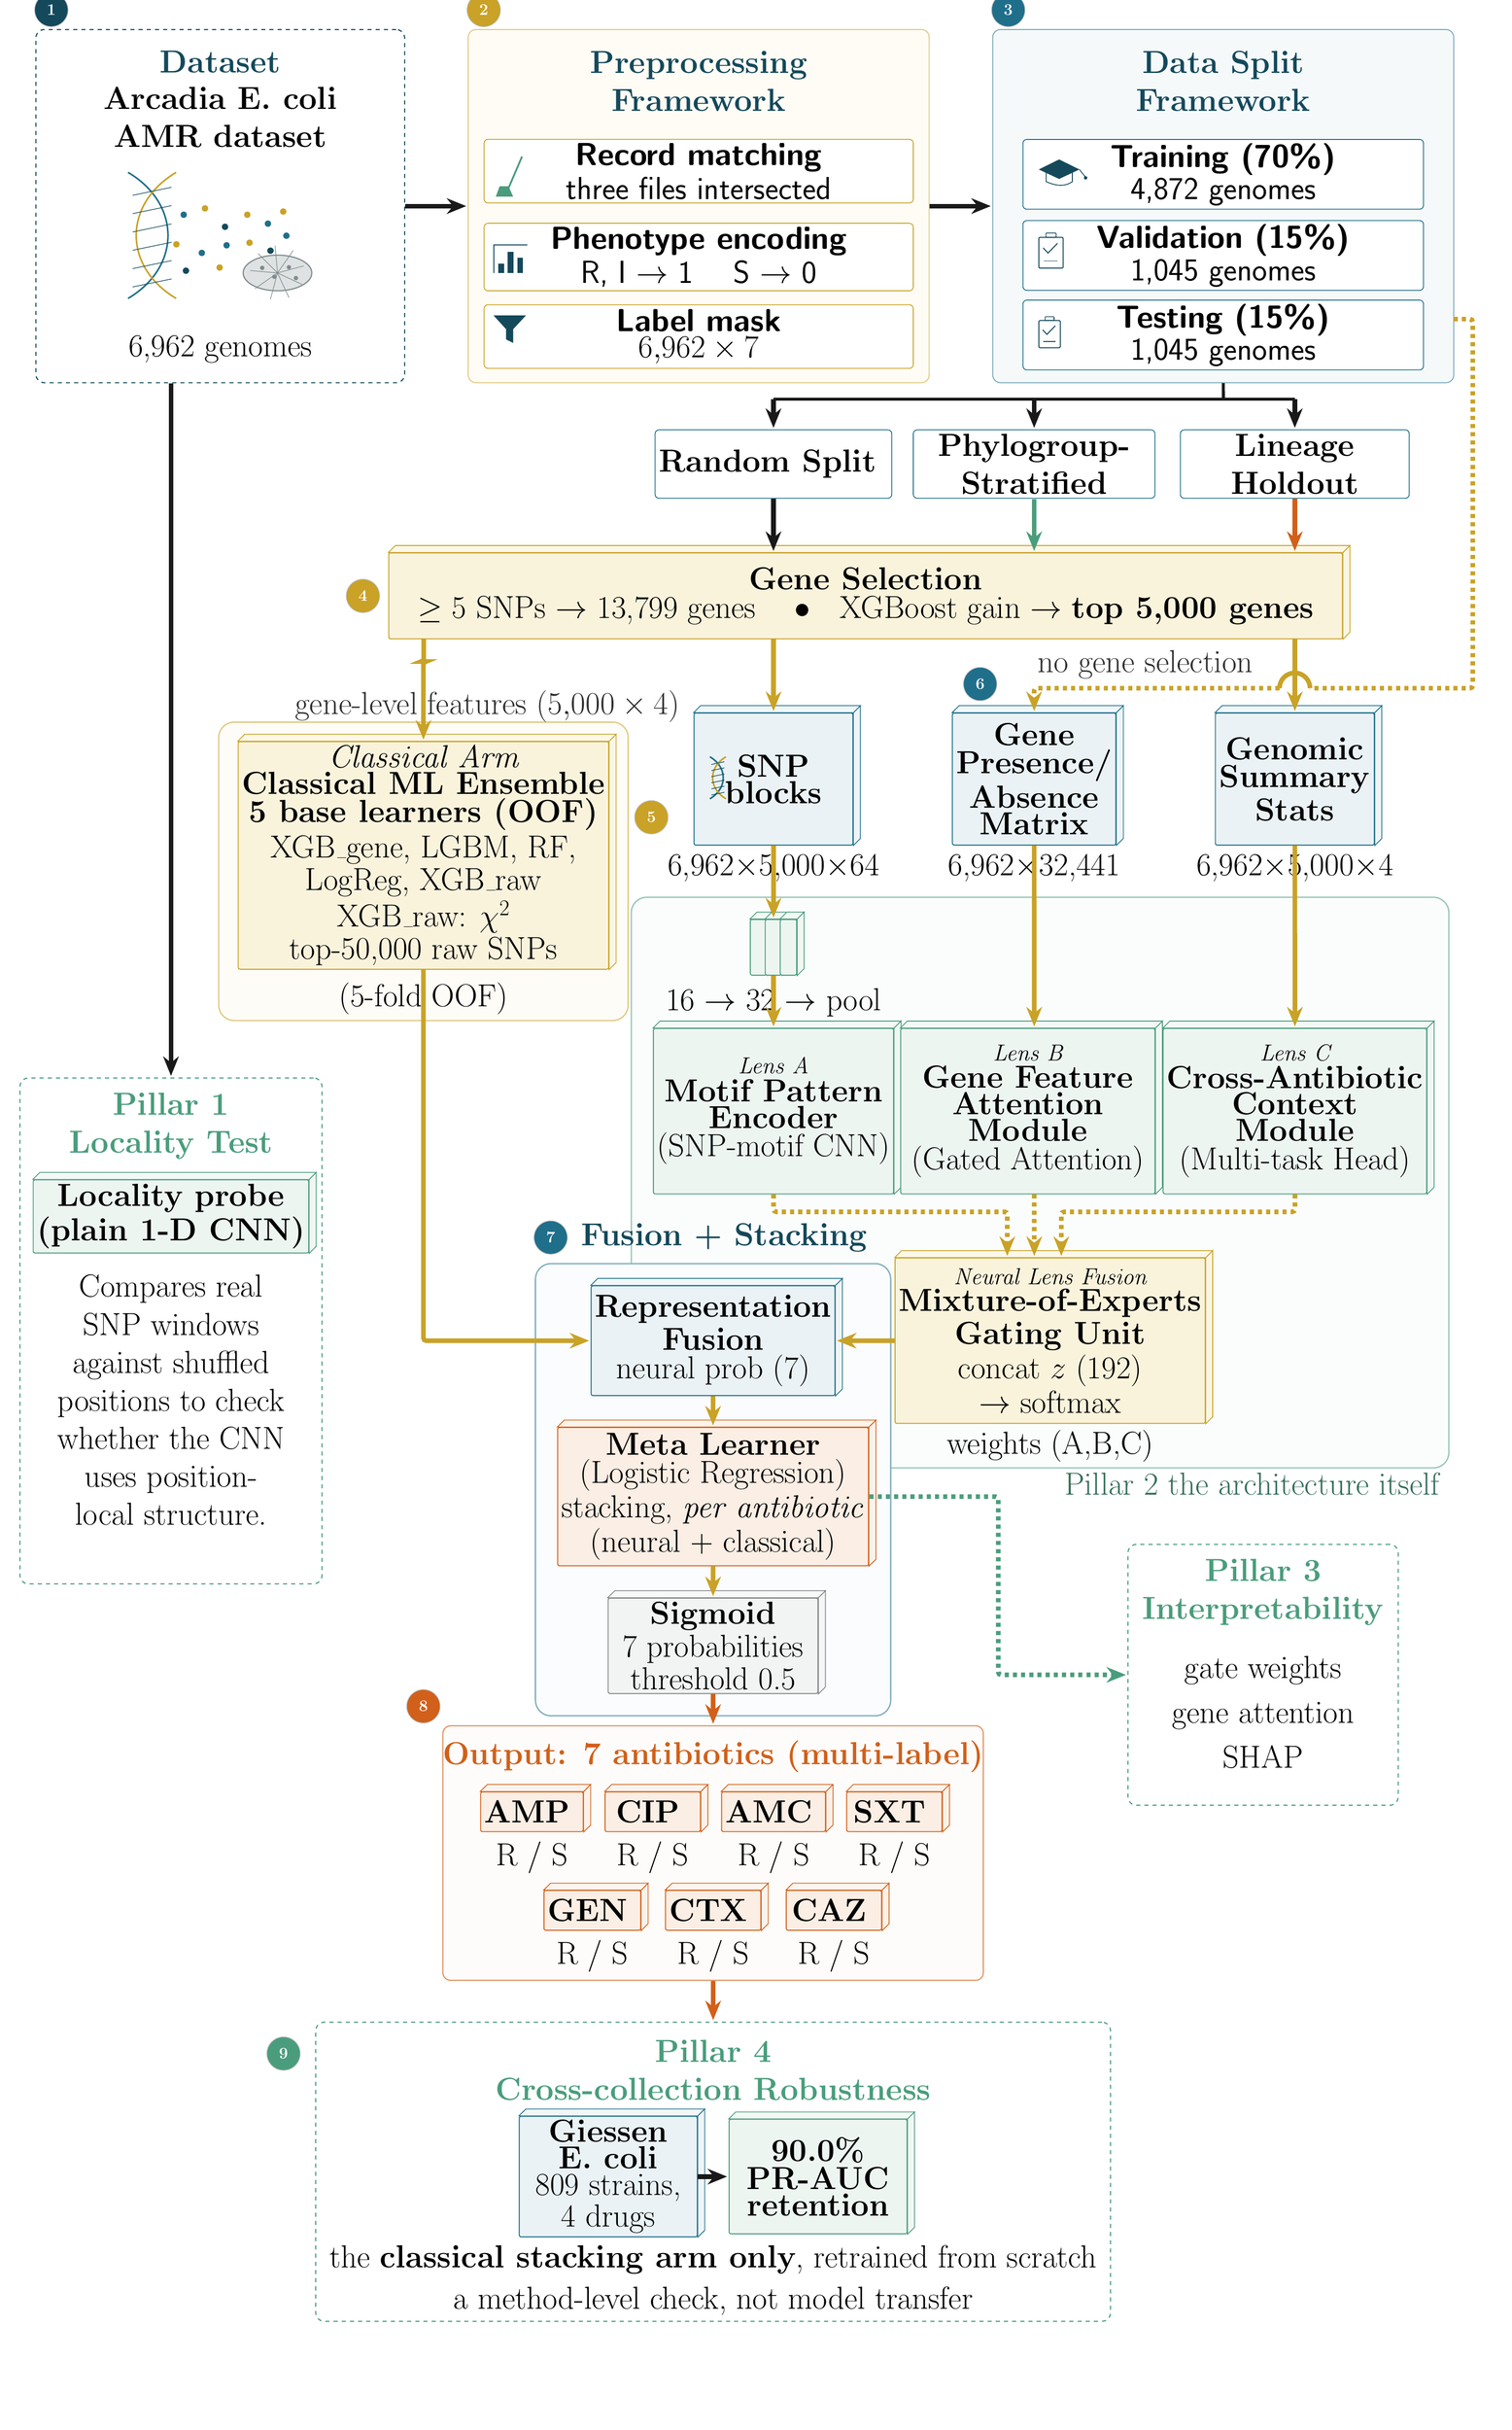
\begin{tikzpicture}[x=1cm,y=1cm,scale=.82,transform shape]
\renewcommand{\Huge}{\fontsize{28.5}{34}\selectfont}
\tikzset{
  arrow/.append style={shorten >=1.2pt, rounded corners=2pt},
  orangeArrow/.append style={shorten >=1.2pt, rounded corners=2pt},
  redArrow/.append style={shorten >=1.2pt, rounded corners=2pt},
  greenArrow/.append style={shorten >=1.2pt, shorten <=0.5pt, rounded corners=2pt},
  % Small numbered "stage" badges + zone corner tags used to make the
  % top-to-bottom reading order of the redesigned pipeline explicit.
  stageBadge/.style args={#1}{circle,fill=#1,text=white,draw=black!25,
    line width=.5pt,font=\bfseries\Large,minimum size=1.05cm,inner sep=0pt},
  zoneTag/.style args={#1}{font=\bfseries\Huge,text=#1!65!black,anchor=west},
}
 
% CHANGED: bounding box nudged to fit the new gene-selection band.
\path[use as bounding box] (-1.00,-45.20) rectangle (45.70,30.30);
 
% Shift the complete pipeline upward while retaining all internal alignments.
\begin{scope}[yshift=1.5cm]
 
% =====================================================================
% Dataset panel
% =====================================================================
\begin{scope}[xshift=2.30cm,yshift=.5cm]
\node[
  dashedPanel,
  draw=navy,
  minimum width=11.6cm,
  minimum height=11.10cm
] (datasetBox) at (3.20,22.25) {};
 
\node[panelTitle,text=navy,anchor=north,font=\bfseries\Huge]
  at (3.20,27.25) {Dataset};
 
\node[font=\bfseries\Huge,align=center]
  at (3.20,25.05) {Arcadia E. coli\\AMR dataset};
 
\DNA{(0.30,19.35)}{1.8}
 
\foreach \x/\y/\c in {
  2.05/23.48/blueedge,
  2.72/23.68/orangeedge,
  3.35/23.10/navy,
  4.05/23.48/orangeedge,
  4.70/23.20/blueedge,
  5.18/23.58/orangeedge,
  1.82/22.55/orangeedge,
  2.62/22.28/blueedge,
  3.40/22.52/blueedge,
  4.12/22.60/orangeedge,
  4.78/22.35/navy,
  5.28/22.82/blueedge,
  2.12/21.72/navy,
  3.18/21.82/orangeedge,
  4.18/21.76/blueedge%
}{
  \fill[fill=\c] (\x,{\y-1.5}) circle (.10);
}
 
\Bacteria{(5.00,20.15)}{2}
 
% CHANGED: the two source deposits are flagged, because they feed two
% different views. Only "Release 2" is a name the thesis uses (Section
% 4.3.2.2); the variant-call deposit is left unnamed rather than guessed at.
\node[font=\Huge,align=center] at (3.20,17.75) {6,962 genomes};
\end{scope}
 
% =====================================================================
% Pre-processing panel
% CHANGED: this panel used to read "Cleaning + deduplication / duplicates
% removed", "Normalization Z=(X-mu)/sigma" and "Feature reduction:
% constant + correlation filter". None of those three appears anywhere in
% the thesis: Section 4.3.1 says the genomes needed no cleaning, no
% z-scoring is described, and the real filters are the two in Section
% 4.3.4 (which have now moved below the split, where they belong).
% =====================================================================
\begin{scope}[xshift=7.55cm,yshift=.5cm]
\node[
  rounded corners=2mm,
  draw=orangeedge!60,
  fill=orangefill!28,
  line width=.7pt,
  minimum width=14.5cm,
  minimum height=11.10cm
] (preBox) at (13,22.25) {};
 
\node[panelTitle,text=navy,anchor=north,font=\bfseries\Huge,align=center]
  at (13,27.25) {Preprocessing\\Framework};
 
\node[
  card=orangeedge,
  minimum width=13.5cm,
  minimum height=2.0cm
] (matchCard) at (13,23.35) {
  \bfseries\Huge{Record matching}\\[4pt]
  \Huge three files intersected
};
 
\node[
  card=orangeedge,
  minimum width=13.5cm,
  minimum height=2.0cm
] (labelCard) at (13,20.65) {
  \bfseries\Huge{Phenotype encoding}\\[4pt]
  \Huge R, I $\rightarrow$ 1 \quad S $\rightarrow$ 0
};
 
\node[
  card=orangeedge,
  minimum width=13.5cm,
  minimum height=2.0cm
] (maskCard) at (13,18.15) {
  \bfseries\Huge{Label mask}\\[4pt]
  \Huge $6{,}962\times7$
};
 
\Broom{(6.55,22.55)}{.85}
\Bars{(6.55,20.15)}{.85}
\Funnel{(6.55,17.95)}{.75}
\end{scope}
 
\draw[arrow] (datasetBox.east) -- (preBox.west);
 
% =====================================================================
% Data split panel
% =====================================================================
\begin{scope}[xshift=12.25cm,yshift=.5cm]
\node[
  rounded corners=2mm,
  draw=blueedge!60,
  fill=bluefill!48,
  line width=.7pt,
  minimum width=14.5cm,
  minimum height=11.10cm
] (splitPanelBox) at (24.8,22.25) {};

\node[panelTitle,text=navy,anchor=north,font=\bfseries\Huge,align=center]
  at (24.8,27.25) {Data Split\\Framework};

\node[
  card=blueedge,
  minimum width=12.6cm,
  minimum height=2.0cm
] (training) at (24.8,23.25) {
  \bfseries\Huge{Training (70\%)}\\[2pt]
  \Huge 4,872 genomes
};

\node[
  card=blueedge,
  minimum width=12.6cm,
  minimum height=2.0cm
] (validation) at (24.8,20.7) {
  \bfseries\Huge{Validation (15\%)}\\[2pt]
  \Huge 1,045 genomes
};

\node[
  card=blueedge,
  minimum width=12.6cm,
  minimum height=2.0cm
] (testing) at (24.8,18.2) {
  \bfseries\Huge{Testing (15\%)}\\[2pt]
  \Huge 1,045 genomes
};

\GradCap{(19,22.85)}{.85}
\Clipboard{(19,20.3)}{.85}
\Clipboard{(19,17.8)}{.75}


\end{scope}

\node[
  minimum width=12.9cm,
  minimum height=8.9cm,
  inner sep=0pt
] (splitBox) at (31.1,22.1) {};

% Data-splitting strategies
\node[
  card=blueedge,
  minimum width=6.6cm,
  minimum height=2.15cm,
  font=\bfseries\Huge
] (randomSplit) at ([xshift=-8.2cm,yshift=-3cm]splitBox.south) {
  Random Split
};

\node[
  card=blueedge,
  minimum width=7.6cm,
  minimum height=2.15cm,
  font=\bfseries\Huge
] (phylogroupSplit) at ([yshift=-3cm]splitBox.south) {
  Phylogroup-\\Stratified
};

\node[
  card=blueedge,
  minimum width=7.2cm,
  minimum height=2.15cm,
  font=\bfseries\Huge
] (lineageHoldout) at ([xshift=8.2cm,yshift=-3cm]splitBox.south) {
  Lineage\\Holdout
};

% One shared trunk from the centre of the Data Split panel's bottom edge,
% forked to the three splitting strategies. Pin the start to the panel frame
% explicitly so it cannot appear to originate from the Testing card.
\coordinate (splitStrategyStart) at
  (splitPanelBox.south);
\coordinate (splitStrategyFork) at
  ([yshift=-0.5cm]splitStrategyStart);
\draw[line] (splitStrategyStart) -- (splitStrategyFork);
\draw[line]
  (randomSplit.north |- splitStrategyFork) --
  (lineageHoldout.north |- splitStrategyFork);
\draw[arrow]
  (randomSplit.north |- splitStrategyFork) -- (randomSplit.north);
\draw[arrow]
  (phylogroupSplit.north |- splitStrategyFork) -- (phylogroupSplit.north);
\draw[arrow]
  (lineageHoldout.north |- splitStrategyFork) -- (lineageHoldout.north);

\draw[arrow] (preBox.east) -- (splitPanelBox.west |- preBox.east);
 
% =====================================================================
% CHANGED -- NEW STAGE: gene selection, AFTER the split.
%
% This is the single most important correction. The old figure put
% "Feature reduction" inside the pre-processing panel, i.e. BEFORE the
% split, which is exactly the leaked pipeline the thesis says it found and
% fixed (Section 4.3.5: "re-fitted on each split's training partition
% instead of being computed only once ... The definition of the pipeline
% used an earlier version that leaked information between splits, which
% was fixed prior to any results in this thesis").
% =====================================================================
\PNBlock{stage15}{(25.8,10.5)}{30cm}{2.70cm}{orangefill}{orangeedge}{
  \Huge\textbf{Gene Selection}\\[5pt]
  \Huge $\ge$ 5 SNPs $\rightarrow$ 13,799 genes
  \quad$\bullet$\quad
  XGBoost gain $\rightarrow$ \textbf{top 5,000 genes}
}
 
 
% Straight arrows carry the three split protocols into gene selection.
\draw[arrow]
  (randomSplit.south) -- (randomSplit.south |- stage15.north);
\draw[greenArrow]
  (phylogroupSplit.south) -- (phylogroupSplit.south |- stage15.north);
\draw[redArrow]
  (lineageHoldout.south) -- (lineageHoldout.south |- stage15.north);
 
% =====================================================================
% Genomic input blocks
% CHANGED: pushed down to make room for the gene-selection band, and now
% fed from it rather than straight from the split.
% =====================================================================
\def\genomicViewWidth{5cm}
\def\genomicViewHeight{4.15cm}
\coordinate (genomicViewRow) at ([yshift=-12.90cm]splitBox.south);
 
\PNBlock{snp}{([xshift=-8.2cm]genomicViewRow)}{\genomicViewWidth}{\genomicViewHeight}{bluefill}{blueedge}{
  \Huge\textbf{SNP}\\[3pt]
  \Huge\textbf{blocks}
}
\PNCaption{snp}{\Huge 6,962$\times$5,000$\times$64}
\DNA{([xshift=-2cm,yshift=-.62cm]snp.center)}{.60}
 
\PNBlock{gene}{(genomicViewRow)}{\genomicViewWidth}{\genomicViewHeight}{bluefill}{blueedge}{
  \Huge\textbf{Gene}\\[3pt]
  \Huge\textbf{Presence/}\\[3pt]
  \Huge\textbf{Absence}\\[3pt]
  \Huge\textbf{Matrix}
}
\PNCaption{gene}{\Huge 6,962$\times$32,441}
 
\PNBlock{summary}{([xshift=8.2cm]genomicViewRow)}{\genomicViewWidth}{\genomicViewHeight}{bluefill}{blueedge}{
  \Huge\textbf{Genomic}\\[4pt]
  \Huge\textbf{Summary}\\[4pt]
  \Huge\textbf{Stats}
}
\PNCaption{summary}{{\Huge 6,962$\times$5,000$\times$4}}
 
% Classical branch. CHANGED: its two distinct inputs are now named -- four
% learners read the gene-level features, XGB_raw reads the chi-squared
% prefiltered raw SNP matrix (Section 4.2.2, Table 4.8).
\PNBlock{ensemble}{([xshift=-8.5cm,yshift=-2.4cm]snp.west)}{11.3cm}{4.80cm}{orangefill}{orangeedge}{
  {\Huge\itshape Classical Arm}\\[3pt]
  \Huge\textbf{Classical ML Ensemble}\\[3pt]
  \Huge\textbf{5 base learners (OOF)}\\[4pt]
  \Huge XGB\_gene, LGBM, RF,\\[3pt]
  \Huge LogReg, XGB\_raw\\[3pt]
  \Huge XGB\_raw: $\chi^2$\\[3pt]
  \Huge top-50,000 raw SNPs
}
 
\node[font=\Huge,anchor=north]
  at ([yshift=-.28cm]ensemble.south) {(5-fold OOF)};
 
% CHANGED: gene selection feeds only the two views that are built from the
% selected 5,000 genes, plus the classical arm's gene-level feature matrix
% (Section 4.1, "the identical gene features feed five base learners";
% Figure 4.4 shows that matrix as 5,000 genes x 4 stats).
\draw[orangeArrow] (snp.north     |- stage15.south) -- (snp.north);
\draw[orangeArrow] (summary.north |- stage15.south) -- (summary.north);
\draw[orangeArrow] (11.9,0 |- stage15.south) -- ++(0,-0.7) -| (ensemble.north);
\node[font=\Huge,anchor=south,text=black!82]
  at (13.9,6.4) {gene-level features ($5{,}000\times4$)};
 
% CHANGED: the pan-genome view is NOT filtered -- release 2 keeps all 32,441
% loci (Section 4.3.2.2, Table 4.6), so it goes round the band, not through it.
% a line-jump keeps it unmistakable that this path ends at the pan-genome
% view only -- it merely passes over the per-gene-statistics arrow.
\draw[draw=orangeedge,line width=3.4pt,dashed,rounded corners=2pt]
  (44.30,19.20) -- (44.90,19.20) -- (44.90,7.60) -- (39.78,7.60);
\draw[draw=orangeedge,line width=3.4pt]
  (39.78,7.60) arc (0:180:0.48);
\draw[orangeArrow,dashed]
  (38.82,7.60) -- (31.10,7.60) -- (gene.north);
\node[font=\Huge,anchor=south,text=black!82]
  at (34.60,7.78) {no gene selection};
 
% CNN stack fed by the SNP blocks.
\PNBlock{cnnOne}{([xshift=-.47cm,yshift=-3.2cm]snp.south)}{.52cm}{1.75cm}{greenfill}{greenedge}{}
\PNBlock{cnnTwo}{([yshift=-3.2cm]snp.south)}{.52cm}{1.75cm}{greenfill}{greenedge}{}
\PNBlock{cnnThree}{([xshift=.47cm,yshift=-3.2cm]snp.south)}{.52cm}{1.75cm}{greenfill}{greenedge}{}
 
\node[font=\Huge,anchor=north]
  at ([yshift=-.28cm]cnnTwo.south) {16 $\rightarrow$ 32 $\rightarrow$ pool};
 
\draw[orangeArrow] (snp.south) -- (cnnTwo.north);
 
% Align the three neural modules beneath their corresponding genomic views.
\def\neuralModuleWidth{6.75cm}
\def\neuralModuleHeight{5.20cm}
\coordinate (neuralModuleRow) at ([yshift=-8.35cm]gene.south);

\PNBlock{motif}{(snp.center |- neuralModuleRow)}{\neuralModuleWidth}{\neuralModuleHeight}{greenfill}{greenedge}{
  {\huge\itshape Lens A}\\[4pt]
  \Huge\textbf{Motif Pattern}\\[3pt]
  \Huge\textbf{Encoder}\\[3pt]
  \Huge(SNP-motif CNN)
}

\PNBlock{attention}{([xshift=-.2cm]gene.center |- neuralModuleRow)}{8cm}{\neuralModuleHeight}{greenfill}{greenedge}{
  {\huge\itshape Lens B}\\[4pt]
  \Huge\textbf{Gene Feature}\\[3pt]
  \Huge\textbf{Attention}\\[3pt]
  \Huge\textbf{Module}\\[3pt]
  \Huge(Gated Attention)
}

\PNBlock{context}{(summary.center |- neuralModuleRow)}{\neuralModuleWidth}{\neuralModuleHeight}{greenfill}{greenedge}{
  {\huge\itshape Lens C}\\[4pt]
  \Huge\textbf{Cross-Antibiotic}\\[3pt]
  \Huge\textbf{Context}\\[3pt]
  \Huge\textbf{Module}\\[3pt]
  \Huge(Multi-task Head)
}

 
% Connect each genomic input to its corresponding neural module.
\draw[orangeArrow] (cnnTwo.south) -- (motif.north);
\draw[orangeArrow] (gene.south) -- ([xshift=.2cm]attention.north);
\draw[orangeArrow] (summary.south) -- (context.north);
 
% Mixture-of-Experts gating unit fed by all three neural modules.
% CHANGED: the gate weights are per sample AND per antibiotic -- without
% that, the box reads as an ordinary static three-way ensemble.
\PNBlock{gate}{([xshift=.7cm,yshift=-4.60cm]attention.south)}{9.6cm}{5.20cm}{orangefill}{orangeedge}{
  {\huge\itshape Neural Lens Fusion}\\[3pt]
  \Huge\textbf{Mixture-of-Experts}\\[3pt]
  \Huge\textbf{Gating Unit}\\[3pt]
  \Huge concat $z$ (192)\\[3pt]
  \Huge$\rightarrow$ softmax
}
 
\node[font=\Huge,anchor=north]
  at ([yshift=-.08cm]gate.south)
  {weights (A,B,C)};
 
\coordinate (gateArrowNorth) at ([xshift=-.5cm]gate.north);
\coordinate (gateArrowWest) at ([xshift=-.5cm]gate.west);
 
\draw[orangeArrow,dashed]
  (motif.south) -- ++(0,-.55) -| ([xshift=-.85cm]gateArrowNorth);
\draw[orangeArrow,dashed]
  ([xshift=.2cm]attention.south) -- (gateArrowNorth);
\draw[orangeArrow,dashed]
  (context.south) -- ++(0,-.55) -| ([xshift=.85cm]gateArrowNorth);
 
% Fuse the seven neural probabilities produced by the gated experts.
\coordinate (pipelineCenterLine) at (21,0);
\PNBlock{fusion}{(pipelineCenterLine |- gate.center)}{7.4cm}{3.45cm}{bluefill}{blueedge}{
  \Huge\textbf{Representation}\\[3pt]
  \Huge\textbf{Fusion}\\[3pt]
  \Huge neural prob (7)
}
 
\draw[orangeArrow] (gate.west) -- (fusion.east);
 
% Stacking meta-learner.
% CHANGED: the six inputs it actually receives are named.
\PNBlock{meta}{([yshift=-4.90cm]fusion.center)}{9.0cm}{4.35cm}{redfill}{rededge}{
  \Huge\textbf{Meta Learner}\\[3pt]
  \Huge(Logistic Regression)\\[3pt]
  \Huge stacking, \emph{per antibiotic}\\[3pt]
  \Huge(neural + classical)
}
 
\draw[orangeArrow] (fusion.south) -- (meta.north);
 
% CHANGED: probability and hard call are separated -- the sigmoid produces
% probabilities (which is what PR-AUC is computed on) and the threshold
% turns them into R/S.
\PNBlock{threshold}{([yshift=-2.50cm]meta.south)}{6.6cm}{3.00cm}{grayfill}{black!48}{
  \Huge\textbf{Sigmoid}\\[3pt]
  \Huge 7 probabilities\\[3pt]
  \Huge threshold 0.5
}
 
\draw[orangeArrow] (meta.south) -- (threshold.north);
 
% Final multi-label output for the seven antibiotics.
\coordinate (outputsBoxCenter) at ($(threshold.south)+(0,-5cm)$);
\node[
  rounded corners=2mm,
  draw=rededge!70,
  fill=redfill!18,
  line width=.8pt,
  minimum width=17cm,
  minimum height=8cm
] (outputsBox) at (outputsBoxCenter) {};
 
\node[
  font=\bfseries\Huge,
  text=rededge,
  anchor=north
] at ([yshift=-.36cm]outputsBox.north) {
  Output: 7 antibiotics (multi-label)
};
 
\foreach \nm/\xx/\yy in {
  AMP/-5.70/1.30,
  CIP/-1.90/1.30,
  AMC/1.90/1.30,
  SXT/5.70/1.30,
  GEN/-3.80/-1.80,
  CTX/0/-1.80,
  CAZ/3.80/-1.80
}{
  \PNBlock{out\nm}{([xshift=\xx cm,yshift=\yy cm]outputsBox.center)}{3.0cm}{1.25cm}{redfill}{rededge}{
    \Huge\textbf{\nm}
  }
 
  \node[font=\Huge,anchor=north]
    at ([yshift=-.18cm]out\nm.south) {R / S};
}
 
\draw[redArrow] (threshold.south) -- (outputsBox.north);
 
% Feed the classical ensemble into the representation-fusion block.
\draw[orangeArrow]
  (ensemble.south) |- (fusion.west);
 
% =====================================================================
% Pillar 1 -- Locality Test.
% CHANGED: moved down (the classical arm now occupies its old row), given
% its pillar number, renamed so it can no longer be confused with Lens A's
% SNP-motif CNN, and its claim softened to what the experiment supports.
% =====================================================================
\node[
  dashedPanel,
  draw=greenedge,
  minimum width=9.5cm,
  minimum height=15.90cm
] (localityBox) at (3.95,-12.60) {};
 
\node[panelTitle,text=greenedge,anchor=north,font=\bfseries\Huge,align=center]
  at ([yshift=-.35cm]localityBox.north) {Pillar 1\\Locality Test};
 
\PNBlock{loccnn}{([yshift=3.60cm]localityBox.center)}{5.80cm}{2.30cm}{greenfill}{greenedge}{
  \bfseries\Huge{Locality probe}\\[3pt]
  \bfseries\Huge{(plain 1-D CNN)}
}
 
\node[
  anchor=north,
  align=center,
  font=\Huge,
  text width=7.4cm
] at ([yshift=-.55cm]loccnn.south) {
  Compares real SNP windows against shuffled positions to check whether the
  CNN uses position-local structure.
};
 
\draw[arrow]
  (datasetBox.south -| localityBox.north) -- (localityBox.north);
 
% =====================================================================
% Pillar 3 -- Interpretability.
% CHANGED: NEW panel. The caption promises four pillars and the old figure
% showed two; this is the one the thesis leans on most heavily
% (Section 5.6.1) and it was entirely absent.
% =====================================================================
\node[
  dashedPanel,
  draw=greenedge,
  minimum width=8.50cm,
  minimum height=8.20cm
] (interpBox) at ([xshift=12.4cm,yshift=-5.6cm]meta.east) {};
 
\node[panelTitle,text=greenedge,anchor=north,font=\bfseries\Huge,align=center]
  at ([yshift=-.35cm]interpBox.north) {Pillar 3\\Interpretability};
 
\node[
  anchor=north,
  align=center,
  font=\Huge,
  text width=7.4cm
] at ([yshift=-3.4cm]interpBox.north) {
  gate weights\\[6pt]
  gene attention\\[6pt]
  SHAP\\[6pt]
};
 
% Straight-segment S-shaped link from the meta learner to Pillar 3.
\coordinate (interpLinkBend) at ($(meta.east)!0.5!(interpBox.west)$);
\draw[greenArrow,dashed]
  (meta.east) -- (interpLinkBend |- meta.east)
  -- (interpLinkBend |- interpBox.west) -- (interpBox.west);
 
% =====================================================================
% Pillar 4 -- independent collection.
% CHANGED: "same TriLens methodology applied to an independent dataset" is
% not what happened -- Table 5.12's own caption says neither column is the
% full TriLens model, and Section 5.5.4 says the three lenses cannot be
% run on Giessen at all. Retention corrected 90.4% -> 90.0% (Table 5.12).
% =====================================================================
\node[
  dashedPanel,
  draw=tealedge,
  minimum width=25.00cm,
  minimum height=9.40cm
] (externalBox) at ([yshift=-6.0cm]outputsBox.south) {};
 
\draw[redArrow] (outputsBox.south) -- (externalBox.north);
 
\node[
  font=\bfseries\Huge,
  text=tealedge,
  anchor=north,
  align=center,
  text width=16.25cm
] at ([yshift=-.45cm]externalBox.north) {
  Pillar 4\\
  Cross-collection Robustness
};
 
\PNBlock{giessen}{([xshift=-3.3cm,yshift=-.15cm]externalBox.center)}{5.60cm}{3.60cm}{bluefill}{blueedge}{
  \Huge\textbf{Giessen}\\[3pt]
  \Huge\textbf{E. coli}\\[4pt]
  \Huge 809 strains,\\[2pt]
  \Huge 4 drugs
}
 
\PNBlock{retention}{([xshift=3.3cm,yshift=-.15cm]externalBox.center)}{5.60cm}{3.60cm}{greenfill}{greenedge}{
  \Huge\textbf{90.0\%}\\[3pt]
  \Huge\textbf{PR-AUC}\\[3pt]
  \Huge\textbf{retention}
}
 
\draw[arrow] (giessen.east) -- (retention.west);
 
\node[
  font=\Huge,
  align=center
] at ([yshift=1.30cm]externalBox.south) {
  the \textbf{classical stacking arm only}, retrained from scratch\\[3pt]
   a method-level check, not model transfer
};
 
% =====================================================================
% Stage-flow guide: tinted zone backgrounds + numbered badges.
% =====================================================================
\begin{scope}[on background layer]
  \coordinate (neuralLensBottom) at ([yshift=-.7cm]gate.south);
  \node[rounded corners=4mm,draw=greenedge!55,fill=greenfill!22,
    line width=1pt,inner sep=16pt,
    fit=(cnnOne)(cnnTwo)(cnnThree)(motif)(attention)(context)(gate)(neuralLensBottom)]
    (neuralLensZone) {};
  \coordinate (classicalLensBottom) at ([yshift=-1cm]ensemble.south);
  \node[rounded corners=4mm,draw=orangeedge!55,fill=orangefill!22,
    line width=1pt,inner sep=14pt,
    fit=(ensemble)(classicalLensBottom)] (classicalLensZone) {};
  \node[rounded corners=4mm,draw=blueedge!55,fill=bluefill!20,
    line width=1pt,inner sep=16pt,
    fit=(fusion)(meta)(threshold)] (decisionZone) {};
\end{scope}
 
\node[stageBadge=navy] at ([xshift=5mm,yshift=6mm]datasetBox.north west) {1};
\node[stageBadge=orangeedge] at ([xshift=5mm,yshift=6mm]preBox.north west) {2};
\node[stageBadge=blueedge] at ([xshift=5mm,yshift=6mm]splitPanelBox.north west) {3};
 
% CHANGED: Stage 1.5 gets its own badge, because it is now its own stage.
\node[stageBadge=orangeedge] at ([xshift=-8mm]stage15.west) {4};
\node[stageBadge=orangeedge] (badge5) at ($(ensemble.east)!0.5!(snp.west)$) {5};
\node[stageBadge=blueedge] at ([xshift=-1.7cm,yshift=9mm]gene.north) {6};
 
\node[stageBadge=blueedge] (badge7) at ([xshift=5mm,yshift=8mm]decisionZone.north west) {7};
\node[zoneTag=blueedge] at ([xshift=3mm]badge7.east) {Fusion + Stacking};
 
% CHANGED: Pillar 2 is the architecture itself, so it is tagged on the
% model zone rather than being left unlabelled.
\node[font=\Huge,text=greenedge!70!black,anchor=north east,align=right]
  at ([xshift=-2mm]neuralLensZone.south east) {
  Pillar 2 the architecture itself\\[2pt]
};
 
\node[stageBadge=rededge] at ([xshift=-6mm,yshift=6mm]outputsBox.north west) {8};
\node[stageBadge=tealedge] at ([xshift=-1cm,yshift=-1cm]externalBox.north west) {9};
 
\end{scope}
 
\end{tikzpicture}
  \end{adjustbox}
  \vspace{-1.5cm}
  \caption{Overview of the proposed system: preprocessing and splitting, the three-view feature extraction and classification framework, and the four evaluation pillars.}
  \label{fig:overview}
\end{figure}

Figure~\ref{fig:overview} shows the entire pipeline, starting with a raw public dataset, preprocessing, and feature building to TriLens-MoE-Stack and eventually to a per-antibiotic resistance prediction. This design is structured around four pillars which also underpin this research: a locality test which rationalises the neural design, the architecture itself, an interpretability study and a cross-dataset generalisation study. Each stage is briefly described in this section and the components are elaborated on in the sections following. The retention figure quoted in the fourth pillar of that diagram is derived in Chapter~\ref{ch:results}.


The pipeline starts with an open-source genomic resource released by Arcadia Science~\cite{arcadia2024}, which associates the genotype of each strain with its resistance phenotype that has been experimentally determined in the laboratory. Since the raw files could not be directly used in machine learning, we joined the genotype and phenotype records, standardised the column names, eliminated duplicates and incomplete records, and coded the resistance labels as integers. There are approximately 7,000 bacterial strains in the published dataset. Among them, 6{,}962 have complete genotype and phenotype data. These strains were used in our study. From the available labels, we chose seven antibiotics which had an acceptable ratio between resistant and susceptible samples, namely ampicillin (AMP), ciprofloxacin (CIP), amoxicillin-clavulanate (AMC), trimethoprim-sulfamethoxazole (SXT), gentamicin (GEN), cefotaxime (CTX) and ceftazidime (CAZ). Figure~\ref{fig:label_overview}
shows how much resistance and label coverage each of the seven has.

\begin{figure}[htb]
\centering
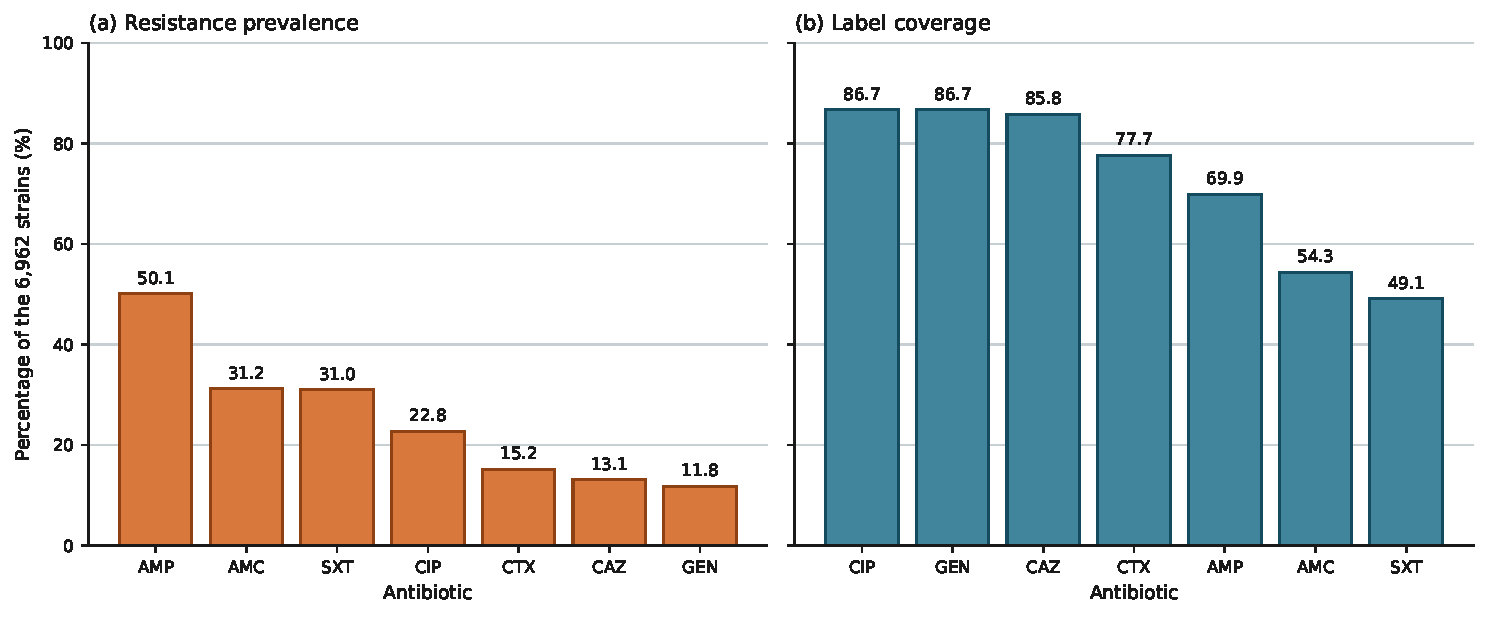
\includegraphics[width=\textwidth]{fig_label_overview.pdf}
\caption{Resistance prevalence and label coverage for the seven retained antibiotics.}
\label{fig:label_overview}
\fignote{\textbf{(a)} Resistance prevalence, ranging from 11.8\% for gentamicin to
50.1\% for ampicillin. \textbf{(b)} Label coverage; no antibiotic carries a label
for more than 86.7\% of the genomes. Both panels share a 0 to 100 per cent axis so
the two quantities can be compared directly.}
\end{figure}


In the cleaned dataset we have built three different genomic views which are complementary to each other, such that the model is not based on one representation. The first is a collection of single-nucleotide polymorphism (SNP) blocks, by gene, of shape $6{,}962 \times 5{,}000 \times 64$, obtained following a two-step gene filter: a variability filter (kept only genes with at least five SNPs), which reduced 18{,}975 genes to 13{,}799, and an importance filter (ranked by gradient-boosting gain), which retained the top 5{,}000 genes. These combined brought 535{,}439 SNPs to 262{,}225, or about 49 percent of the original variants. The second view is a gene presence/absence profile with shape $6{,}962 \times 32{,}441$, which captures resistance genes carried on mobile genetic elements. The third is a collection of shape $6{,}962 \times 5{,}000 \times 4$ per-gene summaries. The filter and all three views are provided in Section~\ref{sec:data}.

The processed data were split into three parts, a training set of 4{,}872 strains, a validation set of 1{,}045 strains and a test set of 1{,}045 strains, about a 70/15/15 split. The lineage holdout below assigns whole groups and so lands on slightly different sizes; Table~\ref{tab:splits} gives the exact figures for all three. The random split randomly assigns strains, thus related strains can be found on both sides. The phylogroup-stratified split preserves an equal distribution of the eight phylogroups in each split. But each phylogroup is present in both the training and test sets. This test, then, does not measure generalisation to unseen lineages but simply the effect of the composition of the lineages. The more challenging question is answered by the sequence-type lineage hold-out split. In this split, any test strain is not of the same sequence type as one of the training strains. All three are described in Section~\ref{sec:comparisons}, including the reason that the phylogroup-stratified split alone was insufficient.

TriLens-MoE-Stack is at the center of the system. It has a feature extractor to extract features from each genomic view and pass them to a separate neural lens. The SNP blocks are fed into a convolutional network called the Motif Pattern Encoder, which identifies small and local mutation patterns in each gene. The gene presence profile goes to the Gene Feature Attention Module, which is a gated-attention network that focuses on the most informative genes. The per-gene statistics are sent to a multi-task head called the Cross-Antibiotic Context Module which provides the ability to share information across similar drugs and helps drugs with fewer labelled examples. The lenses produce a small summary vector and seven per-antibiotic scores.

A Mixture-of-Experts Gating Unit is used to concatenate the three representations into a single 192-length vector. This vector goes through a small network, followed by a softmax. It calculates the weight for each lens individually for each sample and each antibiotic. Consequently, the model is able to use various lenses for a variety of drugs. Simultaneously, the identical gene features feed five base learners, XGBoost on gene features, LightGBM, Random Forest, Logistic Regression, and XGBoost on raw features, each of which makes out-of-fold predictions using five-fold cross-validation. A logistic regression meta-learner combines the neural probability with the five classical probabilities per antibiotic, and a threshold transforms the outcome into a resistant or susceptible call. All the seven antibiotics are forecasted as a multi-label task. The neural lenses are a continuation of a prior GeneAttentionNet precursor that achieved an average precision-recall AUC of approximately 0.769 and supplies the attention signal used later for interpretation.

We present the evaluation using four main pillars. Pillar 1 is concerned with locality. It supports the idea behind the Motif Pattern Encoder. A simple one-dimensional CNN on the entire pan-genome sequence fails the position-shuffling test. This demonstrates that positional locality does not hold across the entire genome. Convolution, however, is more effective within gene blocks. The architecture is Pillar 2. Pillar 3 is interpretability, taken from the model itself through its attention and gating weights and contrasted with post-hoc attribution. The fourth pillar is cross-dataset generalisation, which uses the same methodology on an independent Giessen \textit{E. coli} collection. We are looking for a measure of the success of the system, not only in terms of the correct prediction of resistance, but also one that is appropriate for imbalanced data, primarily precision-recall AUC supported by clinical error rates, so that we will measure how much of the accuracy of the system represents genuine mechanism and how much of it represents population structure.


\FloatBarrier
\section{Preliminary Design and Model Specification}
\label{sec:architecture}

The proposed model TriLens-MoE-Stack is a hybrid architecture in which a stacking meta-learner
is used to join classical machine learning models with neural lenses. The name illustrates the
design: \textit{TriLens} comes from the three genome perspectives the model uses. \textit{MoE} stands
for Mixture of Experts, where a gate determines how much each view should contribute.
\textit{Stack} refers to how the outputs of multiple classical models are combined to produce
the final prediction. The concept is that a bacterial genome can be defined in more
than a single manner and no single definition is complete by itself. A mutation-based view
will miss a resistance gene that arrived on a plasmid, because such a gene is not a mutation at
all. It is simply present, or it is not. A point mutation in a target enzyme is not detectable by the gene presence view. This is
because the gene is present in both resistant and susceptible strains. The only difference is
a single nucleotide change. Instead of selecting between these views, our design incorporates all three and defers to the
model to determine the importance of each view for each antibiotic.


\begin{figure}[H]
  \centering
  \resizebox{0.86\textwidth}{!}{\includestandalone{images/pnn_overall}}
  \caption{Overall dataflow of TriLens-MoE-Stack: three genomic views feed three lenses, which the mixture-of-experts gate fuses before stacking with five classical base learners.}
  \label{fig:trilens-overall}
\end{figure}


This system has three components and the entire architecture is presented in
Figure~\ref{fig:trilens-overall}. To begin with, the three genomic views are processed by a
neural feature extractor that uses three specialised lenses and combines them with a
mixture-of-experts gate. We then use the gene features to train five classical base learners. They make leak-free
out-of-fold predictions. Third, a logistic-regression meta-learner
combines the neural and the classical predictions into a single per-antibiotic prediction.

In the model, each component generates a raw score $z$, whose value may be any real
number, and the score is converted into a probability in the range 0 to 1 with the help of the
logistic sigmoid function,
\begin{equation}
\sigma(z) = \frac{1}{1 + \exp(-z)},
\label{eq:sigmoid}
\end{equation}

\FloatBarrier
\subsection{Rationale for a Hybrid Design Over a Purely Neural One}
\label{subsec:hybrid}

Combining neural and classical models is one of the most crucial design decisions. We use both
instead of one deep neural network. An apparent solution in the contemporary world would be an end-to-end
trained network. We have experimented with that, and it was not very good, but the reason is
in the form of the data, and not in anything wrong with the network. Deep learning works best
in situations where the number of training examples is significantly larger than the number of
input features; our scenario is the opposite with only 6{,}962 labelled strains and hundreds of
thousands of candidate genomic features. The training data can also be memorised in a model that can utilise all this information. Even
with this number of samples, dropout cannot completely avoid that issue.

Gradient boosted trees are much more suited for this type of data. For a feature containing no
signal, the split predictor will just never consider that feature for a split, and it requires
far fewer examples to train a stable model (in this case). The classical arm, then, is not a
fallback or a leftover baseline, it is a load-bearing part of the final design. Meanwhile,
classical models regard each feature as an independent column: they cannot encode the idea
that various mutations near each other within a single gene function as one pattern, nor that
resistance to one cephalosporin says something about another. Those are precisely the types
of tasks a neural network excels at, meaning that the design pairs both, with each arm
addressing the other's weakness. Chapter~\ref{ch:results} provides the proof: on the random
split the neural arm alone hits 0.781 while the combination 0.849, and under the lineage
holdout the classical learners alone score 0.628 while the full model gets 0.634, but the
neural arm yields only 0.472.

\FloatBarrier
\subsection{Classical Base Learners}

The classical arm comprised five base learners: the XGBoost on the gene-aggregated features
(XGB\_gene), LightGBM, Random Forest, Logistic Regression and a second XGBoost on a
chi-squared-prefiltered raw feature matrix (XGB\_raw). These five are trained in an independent
five fold stacking pipeline, and the five out of fold predictions are provided to the
meta-learner of Section~\ref{subsec:metalearner}; the complete configuration is provided with
the hyper-parameters towards the end of this chapter. Each of the five on their own is
presented as a baseline for the proposed model in Chapter~\ref{ch:results}.

Five models might appear to be more than is needed so it is worth explaining why. Only when models of an ensemble commit a variety of errors does the ensemble work. When two
models commit similar errors, their combination does not give much advantage. It averages just
two similar false forecasts. We thus selected five
learners who fail in various manners. Both XGBoost and LightGBM are gradient boosting methods,
but they expand their trees in different ways, thus overfitting to different aspects of the
data. Random Forests use multiple trees, which are averaged and produced to provide a
low-variance but less sharp model. Logistic Regression is also linear and is unable to model
interactions in any way, but it is highly stable. The second XGBoost does not require
gene-level summaries but instead works with raw single-variant features, thus able to capture
signal that is at a single position and would be lost through aggregation. The five are
differentiated between in the three ways that are relevant here: whether a model is able to
pick up combinations of features or only weighs each feature separately, the extent to which
its predictions change when the training data is perturbed slightly, and whether the model
reads the genome one gene at a time or one variant at a time.

Five-fold cross-validation is used to train each base learner, thus each strain is predicted
using a model that was never trained on it. This is more important than it may sound as a
model trained on the full dataset would give overly high scores when asked to make predictions
and the meta-learner would end up putting too much trust in those inflated predictions. This
leak is avoided by out-of-fold prediction, which is why the weights of the stacking layer can
be believed.

\subsubsection{XGBoost}

The gradient boosting idea~\cite{friedman2001gbm} specialised for speed and scale is
XGBoost~\cite{chen2016xgboost} that builds a prediction from multiple shallow decision trees
one by one, each trained from the residual errors of all preceding trees. The process is
illustrated in Figure~\ref{fig:xgboost-workflow}.

\begin{figure}[H]
  \centering
  \makebox[\textwidth][c]{%
    \resizebox{\textwidth}{!}{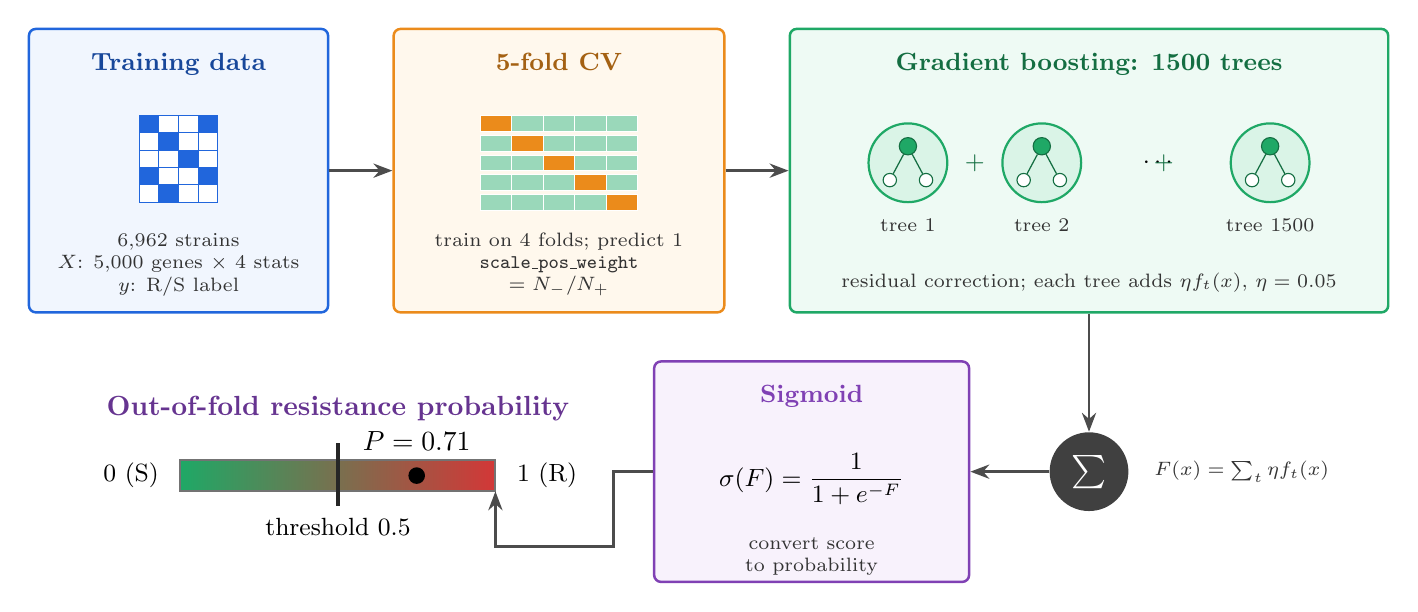
\begin{tikzpicture}[
  font=\sffamily,
  >={Stealth[length=2.4mm]},
  flow/.style={->,draw=black!70,line width=1.05pt},
  title/.style={font=\bfseries\small,align=center},
  label/.style={font=\scriptsize,align=center,text=black!80},
  panel/.style={rounded corners=2.5pt,line width=.9pt,align=center,
                minimum height=36mm,inner sep=4pt,fill opacity=.45},
  tree/.style={circle,draw=xgbgreen,fill=xgbgreenlight,line width=.8pt,
               minimum size=10mm,inner sep=0pt},
  split/.style={circle,draw=xgbdark,fill=xgbgreen,minimum size=2.2mm,
                inner sep=0pt},
  leaf/.style={circle,draw=xgbdark,fill=white,minimum size=1.7mm,
               inner sep=0pt}
]

\definecolor{xgbblue}{RGB}{33,102,220}
\definecolor{xgbbluelight}{RGB}{223,235,253}
\definecolor{xgborange}{RGB}{235,139,27}
\definecolor{xgborangelight}{RGB}{255,239,215}
\definecolor{xgbgreen}{RGB}{31,168,102}
\definecolor{xgbgreenlight}{RGB}{218,244,231}
\definecolor{xgbdark}{RGB}{20,110,66}
\definecolor{xgbpurple}{RGB}{128,65,180}
\definecolor{xgbpurplelight}{RGB}{239,226,249}
\definecolor{xgbred}{RGB}{211,55,55}

\node[panel,draw=xgbblue,fill=xgbbluelight,minimum width=38mm] (data) {};
\node[title,text=xgbblue!70!black,anchor=north] at ([yshift=-2mm]data.north)
  {Training data};
\begin{scope}[shift={([xshift=-5mm,yshift=7mm]data.center)}]
  \foreach \r in {0,...,4}{
    \foreach \c in {0,...,3}{
      \pgfmathtruncatemacro{\on}{mod(2*\r+\c,3)==0 ? 1 : 0}
      \ifnum\on=1
        \fill[xgbblue] (\c*2.5mm,-\r*2.2mm) rectangle ++(2.5mm,-2.2mm);
      \else
        \fill[white] (\c*2.5mm,-\r*2.2mm) rectangle ++(2.5mm,-2.2mm);
      \fi
    }
  }
  \draw[xgbblue,line width=.35pt] (0,0) grid[xstep=2.5mm,ystep=2.2mm] (10mm,-11mm);
\end{scope}
\node[label,anchor=south] at ([yshift=1mm]data.south)
  {6,962 strains\\$X$: 5,000 genes $\times$ 4 stats\\$y$: R/S label};

\node[panel,draw=xgborange,fill=xgborangelight,minimum width=42mm,
      right=8mm of data] (cv) {};
\node[title,text=xgborange!70!black,anchor=north] at ([yshift=-2mm]cv.north)
  {5-fold CV};
\begin{scope}[shift={([xshift=-10mm,yshift=7mm]cv.center)}]
  \foreach \r in {0,...,4}{
    \foreach \c in {0,...,4}{
      \ifnum\r=\c
        \fill[xgborange] (\c*4mm,-\r*2.5mm) rectangle ++(4mm,-2mm);
      \else
        \fill[xgbgreen!45] (\c*4mm,-\r*2.5mm) rectangle ++(4mm,-2mm);
      \fi
      \draw[white,line width=.25pt] (\c*4mm,-\r*2.5mm) rectangle ++(4mm,-2mm);
    }
  }
\end{scope}
\node[label,anchor=south] at ([yshift=1mm]cv.south)
  {train on 4 folds; predict 1\\\texttt{scale\_pos\_weight}\\$=N_-/N_+$};

\node[panel,draw=xgbgreen,fill=xgbgreenlight,minimum width=76mm,
      right=8mm of cv] (boost) {};
\node[title,text=xgbdark,anchor=north] at ([yshift=-2mm]boost.north)
  {Gradient boosting: 1500 trees};

\node[tree] (t1) at ([xshift=-23mm,yshift=1mm]boost.center) {};
\node[tree] (t2) at ([xshift=-6mm,yshift=1mm]boost.center) {};
\node[font=\small] at ([xshift=9mm,yshift=1mm]boost.center) {$\cdots$};
\node[tree] (tn) at ([xshift=23mm,yshift=1mm]boost.center) {};
\foreach \t in {t1,t2,tn}{
  \node[split] (\t-r) at ([yshift=2.1mm]\t.center) {};
  \node[leaf] (\t-l) at ([xshift=-2.3mm,yshift=-2.2mm]\t.center) {};
  \node[leaf] (\t-q) at ([xshift=2.3mm,yshift=-2.2mm]\t.center) {};
  \draw[xgbdark,line width=.45pt] (\t-r)--(\t-l) (\t-r)--(\t-q);
}
\node[label,below=.7mm of t1] {tree 1};
\node[label,below=.7mm of t2] {tree 2};
\node[label,below=.7mm of tn] {tree 1500};
\node[font=\small,text=xgbdark] at ($(t1)!0.5!(t2)$) {$+$};
\node[font=\small,text=xgbdark] at ($(t2)!0.5!(tn)+(1mm,0)$) {$+$};
\node[label,anchor=south] at ([yshift=1.5mm]boost.south)
  {residual correction; each tree adds $\eta f_t(x)$, $\eta=0.05$};

\node[circle,fill=black!75,text=white,minimum size=10mm,font=\large,
      below=15mm of boost] (sum) {$\sum$};
\node[label,anchor=west] at ([xshift=2mm]sum.east)
  {$F(x)=\sum_t\eta f_t(x)$};

\node[panel,draw=xgbpurple,fill=xgbpurplelight,minimum width=40mm,
      minimum height=28mm,left=10mm of sum] (sig) {};
\node[title,text=xgbpurple,anchor=north] at ([yshift=-2mm]sig.north) {Sigmoid};
\node[font=\small] at ([yshift=-.1cm]sig.center)
  {$\displaystyle \sigma(F)=\frac{1}{1+e^{-F}}$};
\node[label,anchor=south] at ([yshift=-0.02cm]sig.south)
  {convert score\\to probability};

\begin{scope}[shift={([xshift=-60mm,yshift=-2.5mm]sig.west)}]
  \node[font=\normalsize\bfseries,align=center,text=xgbpurple!80!black]
    at (20mm,10.5mm)
    {Out-of-fold resistance probability};
  \shade[left color=xgbgreen,right color=xgbred]
    (0,0) rectangle (40mm,4mm);
  \draw[black!55,line width=.7pt] (0,0) rectangle (40mm,4mm);
  \draw[black!85,line width=1.3pt] (20mm,-1.8mm)--(20mm,6.2mm);
  \node[font=\small,align=center] at (20mm,-4.5mm) {threshold 0.5};
  \node[font=\small,anchor=east] at (-1.5mm,2mm) {0 (S)};
  \node[font=\small,anchor=west] at (41.5mm,2mm) {1 (R)};
  \fill[black] (30mm,2mm) circle (3pt);
  \node[font=\normalsize\bfseries,anchor=south] at (30mm,4mm) {$P=0.71$};
  \coordinate (prob-south-east) at (40mm,0);
  \coordinate (prob-route) at (46mm,-7mm);
\end{scope}

\draw[flow] (data.east)--(cv.west);
\draw[flow] (cv.east)--(boost.west);
\draw[flow] (boost.south)--(sum.north);
\draw[flow] (sum.west)--(sig.east);
\draw[flow] (sig.west)--++(-5mm,0) |- (prob-route) -| (prob-south-east);

\end{tikzpicture}
}%
  }
  \caption{XGBoost base learner: five-fold cross-validation, an additive chain of shrunken trees, then a sigmoid giving the out-of-fold probability.}
  \label{fig:xgboost-workflow}
\end{figure}

Formally, the prediction score for a sample $x$ is the sum of the outputs of $T$ trees:
\begin{equation}
\hat{y}(x) = \sum_{t=1}^{T} \eta\, f_t(x),
\label{eq:xgb_score}
\end{equation}
with each $f_t$ being one tree and $\eta$ being a small learning rate, or shrinkage, which
reduces the contribution of each tree in the model to ensure no one tree is dominant and the
model is enhanced in small, steady steps. Training will reduce a loss that is penalised:
\begin{equation}
\mathcal{L} = \sum_{i=1}^{n} \ell(y_i, \hat{y}_i) + \sum_{t=1}^{T} \Omega(f_t),
\label{eq:xgb_loss}
\end{equation}
and $\ell(\cdot)$ is the binary cross-entropy loss on the $\sigma(\hat{y})$ and $\Omega(f_t)$
is the penalty on trees with a large number of leaves or an excessive number of extreme leaf
values, thus any extra complexity must decrease the error by an amount that justifies its cost.

\vspace{1em}

There are two reasons for XGBoost's inclusion in this list as far as this data is concerned.
If a feature has no information, it is not split, thus a tree can represent a very wide
matrix, and if there is a resistance that requires two mutations together, the tree can split
on one and then the other, which no linear model can do. Where susceptible strains greatly outnumber resistant ones for a drug, the
\texttt{scale\_pos\_weight} parameter is set to the ratio between them. A summary of the genome is represented using XGBoost on the gene-aggregated features, while a
fine-grained view is represented by XGBoost on a chi-squared-prefiltered raw matrix. We choose the number of trees using early stopping~\cite{prechelt1998earlystopping}.

XGBoost also differs from plain gradient boosting in that each tree is fitted using the second
derivative of the loss and not the gradient alone, so a leaf resting on a few strains the model
is already confident about is pulled towards zero. The same quantity sets the bar for splitting:
with $\gamma$ at 0.1, a split that separates two strains but barely moves the loss is never taken.

\subsubsection{LightGBM}

LightGBM~\cite{ke2017lightgbm} applies the same boosting concept with a couple important
shortcuts that are particularly relevant when the data is this wide: histogram binning, which
only uses the bin edges when searching for a split point, and leaf-wise growth, where after
each boosting round it expands whichever single leaf most reduces the error rather than growing
level by level. The outcome is a deeper tree in the areas where the data is
sparse. Growing this way needs a ceiling, or the model keeps splitting one branch until it has
isolated single strains, and ours is \texttt{num\_leaves} at 63 against \texttt{max\_depth} at
6, one short of the 64 leaves a full level-wise tree of that depth would carry. The tree can
therefore spend its budget unevenly without ever growing taller than the XGBoost trees it is
meant to disagree with. The workflow is provided on Figure~\ref{fig:lightgbm-workflow}.

\begin{figure}[H]
    \centering
    \resizebox{0.94\textwidth}{!}{% ============================================================
%  LightGBM base-learner workflow  --  antibiotic resistance prediction.
%  Faithful to the config (stage3_cascadestack_v9, used by the v10 stack):
%  X = 5000 genes x 4 stats, y = R/S, histogram binning, F0 = mu,
%  subsample=0.8, colsample_bytree=0.7, subsample_freq=1,
%  num_leaves=63, max_depth=6, min_child_samples=20, reg_alpha/lambda,
%  eta=0.05, ~1500 trees, early_stopping_rounds=150,
%  sum -> sigmoid -> resistance probability at threshold 0.5.
%  Include with:   \input{images/lightgbm_workflow}   (file goes in images/)
%  Requires in main.tex preamble:
%    \usepackage{amsmath}
%    \usepackage{tikz}
%    \usetikzlibrary{arrows.meta,positioning,fit,backgrounds,calc}
% ============================================================

%% ------------------------------------------------------------------ COLOURS
\definecolor{Cnav}{RGB}{18,52,96}
\definecolor{CnavM}{RGB}{30,80,150}
\definecolor{Cblu}{RGB}{58,140,205}
\definecolor{CbluBG}{RGB}{234,246,253}
\definecolor{CgD}{RGB}{26,110,60}
\definecolor{CgM}{RGB}{45,158,88}
\definecolor{CgL}{RGB}{130,205,148}
\definecolor{Cpur}{RGB}{98,54,176}
\definecolor{CdR}{RGB}{204,52,42}
\definecolor{CdB}{RGB}{32,74,188}
\definecolor{CdG}{RGB}{148,158,168}
\definecolor{Chst}{RGB}{60,124,192}
\definecolor{Cpin}{RGB}{20,110,54}
\definecolor{Csg}{RGB}{0,0,0}

\begingroup
%% Only two text sizes are used anywhere in the figure, so nothing can look
%% "small" next to its neighbours:  \Huge = headline,  \LARGE = all body text.
\renewcommand{\Huge}{\fontsize{41}{48}\selectfont}
\renewcommand{\LARGE}{\fontsize{28}{34}\selectfont}

\begin{tikzpicture}[
  font=\sffamily, x=1cm, y=1cm,
  Aarr/.style={-{Stealth[length=22pt,width=16pt,round]},line width=4.0pt,color=black},
  Garr/.style={-{Stealth[length=22pt,width=16pt,round]},line width=4.0pt,color=CgD},
  Darr/.style={-{Stealth[length=20pt,width=15pt,round]},line width=3.4pt,
                dashed,dash pattern=on 11pt off 7pt,color=CgD},
  Box/.style={draw=CnavM,fill=CbluBG,rounded corners=15pt,line width=3.0pt},
  Sell/.style={draw=CgD,fill=white,circle,line width=3.6pt,minimum size=5.6cm,align=center},
  Iball/.style={draw=#1,fill=#1!13,circle,line width=2.4pt,minimum size=62pt,inner sep=0pt},
  Iball/.default=Cblu,
  Cap/.style={align=center,text=Csg,font=\sffamily\LARGE},
  Hd/.style={align=center,font=\sffamily\LARGE,text=CgD},
  Lbl/.style={font=\sffamily\itshape\LARGE,fill=white,inner sep=7pt},
]

% Recenter: the auto bounding box has extra invisible margin on the left
% (ink sits shifted right relative to the resized/centered figure). Force
% a symmetric box up front so the diagram lines up with the body text
% margins (must come before any node/path is drawn to take effect).
\path[use as bounding box] (-28.9pt,-1250.57532pt) rectangle (1467.31628pt,170.63417pt);

%% ================================================================== TITLE

\node[align=center,font=\sffamily\Huge,text=CnavM] at (23.6,1.7)
  {STAGE 1:\\[2pt]HISTOGRAM-BASED PREPROCESSING};
\node[align=center,font=\sffamily\Huge,text=CnavM] at (44,1.7)
  {STAGE 2:\\[2pt]INITIALISATION};

%% ================================================================== INPUT
\node[Box,minimum width=10.5cm,minimum height=11.4cm] (IB) at (3.5,-6.6) {};
\node[font=\sffamily\Huge,text=CnavM] at (3.5,-2.6) {INPUT DATA};

\node[Iball=Cblu] (Ic1) at (0.9,-4.9) {};
\begin{scope}[shift={(0.9,-4.9)}]
  \draw[Cblu,line width=1.5pt] (-0.32,0.17) to[out=52,in=128] (0.32,0.17);
  \draw[Cblu,line width=1.5pt] (-0.32,-0.17) to[out=-52,in=-128] (0.32,-0.17);
  \foreach \x in {-0.17,0,0.17}{\draw[Cblu,line width=1.3pt] (\x,0.21)--(\x,-0.21);}
\end{scope}
\node[right=10pt of Ic1,text=Cnav,font=\sffamily\LARGE,align=left]
  {Genomic\\[-2pt]Features};

\node[Iball=CnavM] (Ic2) at (0.9,-7.2) {};
\begin{scope}[shift={(0.9,-7.2)},scale=2.3]
  \draw[CnavM,line width=1.5pt,fill=white,rounded corners=1.5pt]
    (-0.13,0.15) rectangle (0.13,-0.15);
  \draw[CnavM,line width=1.5pt,fill=CnavM] (-0.06,0.18) rectangle (0.06,0.13);
  \draw[CnavM,line width=1.1pt] (-0.09,0.06)--(0.09,0.06);
  \draw[CnavM,line width=1.1pt] (-0.09,-0.01)--(0.09,-0.01);
  \draw[CnavM,line width=1.1pt] (-0.09,-0.08)--(0.03,-0.08);
\end{scope}
\node[right=10pt of Ic2,text=Cnav,font=\sffamily\LARGE,align=left]
  {Clinical\\[-2pt]Metadata};

\node[Iball=Cpur] (Ic3) at (0.9,-9.5) {};
\begin{scope}[shift={(0.9,-9.5)}]
  \draw[Cpur,line width=1.5pt] (0,0) circle(0.42);
  \filldraw[Cpur!65] (-0.14,0.13) circle(0.082);
  \filldraw[Cpur!65] ( 0.13,0.09) circle(0.082);
  \filldraw[Cpur!65] (-0.09,-0.14) circle(0.082);
  \filldraw[Cpur!65] ( 0.15,-0.15) circle(0.060);
\end{scope}
\node[right=10pt of Ic3,text=Cnav,font=\sffamily\LARGE,align=left]
  {AMR\\[-2pt]Labels};

\node[font=\sffamily\LARGE,text=CnavM] at (3.5,-11.4) {Training dataset};

%% ================================================================== STAGE 1
\node[Box,minimum width=17cm,minimum height=11.4cm] (S1) at (23.6,-6.6) {};
\begin{scope}[shift={(16.2,-9.2)},xscale=0.70,yscale=0.68]
  \fill[Chst!38] (0.0,0) rectangle (1.0,2.3);
  \fill[Chst!62] (1.2,0) rectangle (2.2,3.9);
  \fill[Chst!88] (2.4,0) rectangle (3.4,5.6);
  \fill[Chst]    (3.6,0) rectangle (4.6,4.5);
  \fill[Chst!68] (4.8,0) rectangle (5.8,2.9);
  \draw[Csg!60,line width=1.8pt,->] (-0.3,0)--(6.6,0);
  \draw[Csg!60,line width=1.8pt,->] (-0.3,0)--(-0.3,6.4);
\end{scope}
\node[anchor=west,align=left,text=Csg,font=\sffamily\LARGE] at (21.0,-6.6)
  {$\bullet$\ Histogram Binning\\
   \quad(continuous $\rightarrow$ discrete)\\[9pt]
   $\bullet$\ Handle Missing Values\\[9pt]
   $\bullet$\ Prepare Feature Values\\[9pt]
   $\bullet$\ Construct Histograms};

%% ================================================================== STAGE 2
\node[Box,minimum width=11cm,minimum height=11.4cm] (S2) at (44,-6.6) {};
\node[draw=Cblu,fill=Cblu,circle,minimum size=4.0cm,font=\Huge,text=white]
  (MU) at (44,-4.2) {$\mu$};
\node[align=center,text=Csg,font=\sffamily\LARGE] at (44,-7.9)
  {Initialise base score with\\the average resistance\\rate in the training data};
\node[draw=CnavM!55,fill=white,rounded corners=10pt,line width=2.2pt,
      font=\Huge,inner sep=11pt] at (44,-10.9) {$F_0=\mu$};

\draw[Aarr] (IB.east) -- (S1.west);
\draw[Aarr] (S1.east) -- (S2.west);

%% ================================================================== STAGE 3 FRAME
\node[draw=CgD,fill=white,rounded corners=22pt,line width=4.4pt,
      fit={(-1.0,-14.6) (49.5,-32.3)}] (S3) {};
\node[font=\sffamily\Huge,text=CgD,fill=white,inner sep=8pt] at (24.25,-14.6)
  {STAGE 3: LEAF-WISE ITERATIVE BOOSTING};
\node[draw=CgD,dashed,dash pattern=on 13pt off 8pt,rounded corners=18pt,
      line width=2.6pt,fit={(0.2,-15.9) (38.9,-29.7)}] (INNER) {};

%% ---- the five steps of one boosting iteration -----------------------------
\node[Sell] (E1) at ( 4.0,-21.9) {};
\node[Sell] (E2) at (11.8,-21.9) {};
\node[Sell] (E3) at (19.6,-21.9) {};
\node[Sell] (E4) at (27.4,-21.9) {};
\node[Sell] (E5) at (35.2,-21.9) {};

\node[Hd] at ( 4.0,-17.5) {1. Gradients\\\& Hessians};
\node[Hd] at (11.8,-17.5) {2. Row + Feature\\Subsampling};
\node[Hd] at (19.6,-17.5) {3. Histogram\\Split Finding};
\node[Hd] at (27.4,-17.5) {4. Leaf-wise\\Tree Growth};
\node[Hd] at (35.2,-17.5) {5. Add Scaled\\Tree Output};

% 1 : gradient / hessian scatter
\begin{scope}[shift={(4.0,-21.9)},scale=1.9]
  \draw[Csg!50,line width=1.1pt,->] (-0.78,0)--(0.84,0);
  \draw[Csg!50,line width=1.1pt,->] (-0.66,-0.78)--(-0.66,0.84);
  \foreach \px/\py in {-0.08/0.38,0.16/0.58,0.40/0.22,-0.36/0.12,0.24/-0.14,
                       -0.12/-0.36,0.48/0.46,-0.46/0.42,0.00/-0.56}
    \filldraw[CdG,fill=CdG!55] (\px,\py) circle(3.6pt);
  \foreach \px/\py in {0.36/-0.48,-0.26/0.58}
    \filldraw[CgD,fill=CgM!70] (\px,\py) circle(3.6pt);
\end{scope}

% 2 : subsampling grid
\begin{scope}[shift={(11.8,-21.9)},scale=1.9]
  \foreach \c in {0,2}{\fill[CdB!22] ({-0.66+\c*0.33},-0.66) rectangle ++(0.33,1.32);}
  \foreach \r in {0,1,3}{\fill[CgM!32] (-0.66,{-0.66+\r*0.33}) rectangle ++(1.32,0.33);}
  \foreach \r in {0,...,3}{\foreach \c in {0,...,3}{
     \draw[CdG!60,line width=0.8pt] ({-0.66+\c*0.33},{-0.66+\r*0.33}) rectangle ++(0.33,0.33);}}
  \draw[Csg!60,line width=1.2pt] (-0.66,-0.66) rectangle (0.66,0.66);
\end{scope}

% 3 : split finding
\begin{scope}[shift={(19.6,-21.9)},scale=1.6]
  \foreach \i/\h in {0/0.42,1/0.72,2/1.14,3/0.78,4/0.48}{
     \fill[CgD!55] ({-0.90+\i*0.36},-0.62) rectangle ++(0.29,\h);}
  \draw[Csg!55,line width=1.2pt] (-0.96,-0.62)--(1.02,-0.62);
  \draw[CdR,line width=2.4pt,dashed] (0.06,-0.80)--(0.06,0.80);
\end{scope}

% 4 : leaf-wise tree
\begin{scope}[shift={(27.4,-21.7)},scale=1.4]
  \draw[CgD,line width=2.2pt]
    (0,0.62)--(-0.56,-0.16) (0,0.62)--(0.56,-0.16)
    (-0.56,-0.16)--(-0.84,-0.94) (-0.56,-0.16)--(-0.28,-0.94)
    (0.56,-0.16)--(0.28,-0.94) (0.56,-0.16)--(0.84,-0.94);
  \filldraw[CgD,fill=CgD] (0,0.62) circle(6.6pt);
  \filldraw[CgD,fill=CgM!80] (-0.56,-0.16) circle(5.8pt);
  \filldraw[CgD,fill=CgM!80] (0.56,-0.16) circle(5.8pt);
  \filldraw[CgM!70,fill=CgL!70](-0.84,-0.94) circle(5.2pt);
  \filldraw[CgM!70,fill=CgL!70](-0.28,-0.94) circle(5.2pt);
  \filldraw[CgM!70,fill=CgL!70](0.28,-0.94) circle(5.2pt);
  \filldraw[CgM!70,fill=CgL!70](0.84,-0.94) circle(5.2pt);
  \node[font=\Huge,text=CgD] at (0,-1.42) {$\cdots$};
\end{scope}

% 5 : scaled tree output
\node[draw=CgD,fill=CgD,circle,minimum size=4.3cm,font=\Huge,text=white]
  at (35.2,-21.9) {$\eta f_t(x)$};

%% ---- captions (every line kept short so columns never collide) ------------
\node[Cap] at ( 4.0,-27.0) {$g_i=\partial L/\partial\hat{y}_i$\\[6pt]
                            $h_i=\partial^2 L/\partial\hat{y}_i^{\,2}$};
\node[Cap] at (11.8,-27.0) {rows: $0.8$\\features: $0.7$};
\node[Cap] at (19.6,-27.0) {scan bin edges\\for maximum\\loss reduction};
\node[Cap] at (27.4,-27.0) {num\_leaves $=63$\\max\_depth $\le 6$\\min\_child $=20$\\L1 + L2 penalty};
\node[Cap] at (35.2,-27.0) {$F_t=F_{t-1}+\eta f_t(x)$\\$\eta=0.05$\\up to $1500$ trees};

%% ---- validation / early stopping -----------------------------------------
\node[Hd] at (44.0,-17.5) {Validation Check\\\& Early Stopping};
\node[draw=CgD,fill=white,dashed,dash pattern=on 12pt off 7pt,rounded corners=16pt,
      line width=3.2pt,minimum width=8.5cm,minimum height=6.0cm] (VB) at (44.0,-21.9) {};
\begin{scope}[shift={(42.4,-22.8)},xscale=0.60,yscale=0.42]
  \fill[CgM!88]  (0.00,0) rectangle (0.90,4.5);
  \fill[CgM!100] (1.20,0) rectangle (2.10,6.2);
  \fill[CgM!80]  (2.40,0) rectangle (3.30,5.0);
  \fill[CgM!60]  (3.60,0) rectangle (4.50,3.2);
  \draw[Csg!48,line width=1.8pt,->] (-0.3,0)--(5.4,0);
  \draw[Csg!48,line width=1.8pt,->] (-0.3,0)--(-0.3,7.4);
\end{scope}
% Nudged right (44.0->44.4) so the bolded "rounds with no gain" line clears
% the dashed inner boosting-loop frame to its left instead of touching it.
\node[Cap] at (44.4,-27.0) {stop after $150$\\rounds with no gain};

%% ---- horizontal flow ------------------------------------------------------
\draw[Garr] (E1) -- (E2);
\draw[Garr] (E2) -- (E3);
\draw[Garr] (E3) -- (E4);
\draw[Garr] (E4) -- (E5);
\draw[Garr] (E5) -- (VB.west);

%% ---- entry from Stage 2 -> Stage 3 (Clean horizontal channel & vertical drop) ----
\draw[Aarr,rounded corners=14pt]
  (S2.south) -- (44.0,-13.2) -- (0.8,-13.2) -- (0.8,-15.9);
\node[Lbl,text=Csg] at (22.4,-13.2) {start the boosting loop from $F_0$};

%% ---- feedback loop        -> enters E1 at 200 deg (lower left) --------------
%% Its vertical run sits at x=-0.4 and stops at y=-22.86, so it can never
%% cross the entry arrow, whose horizontal run is at y=-20.94.
\draw[Darr,rounded corners=12pt]
  (40.0,-24.9) -- (40.0,-31.0) -- (-0.4,-31.0) -- (-0.4,-22.86) -- (E1.200);
\node[Lbl,text=CgD] at (20.0,-31.0) {updated gradients: continue with tree $t+1$};

%% ================================================================== OUTPUT ROW
\node[draw=Cpur,fill=white,rounded corners=16pt,line width=3.0pt,
      minimum width=16.5cm,minimum height=9.4cm] (FB) at (5.5,-39.2) {};
\node[font=\sffamily\LARGE,text=Cpur] at (5.5,-36.1) {FINAL ENSEMBLE MODEL};
\node[align=center,font=\Huge] at (5.5,-39.3)
  {$\displaystyle F(x)=\sum_{t=1}^{T}\eta f_t(x)+\mu$};
\node[Cap] at (5.5,-42.5) {Add initial score $\mu$ to\\the sum of all trees};

\node[draw=Cpur,fill=white,rounded corners=16pt,line width=3.0pt,
      minimum width=18cm,minimum height=9.4cm] (SG) at (24.1,-39.2) {};
\node[font=\sffamily\LARGE,text=Cpur] at (24.1,-36.1) {SIGMOID TRANSFORMATION};
\node[align=center,font=\Huge] at (24.1,-39.3)
  {$\displaystyle P(x)=\sigma\!\left(F(x)\right)=\frac{1}{1+e^{-F(x)}}$};
\node[Cap] at (24.1,-42.5) {Convert raw score to\\resistance probability};

\node[draw=Cpur,fill=white,rounded corners=16pt,line width=3.0pt,
      minimum width=15.5cm,minimum height=9.4cm] (DB) at (41.75,-39.2) {};
\node[font=\sffamily\LARGE,text=Cpur] at (41.75,-36.1) {DECISION (THRESHOLD $=0.5$)};
\begin{scope}[shift={(35.05,-39.6)}]
  \shade[left color=Cpin,right color=Cpur] (0,0) rectangle (13.4,1.2);
  \draw[Csg,line width=1.5pt] (0,0) rectangle (13.4,1.2);
  \draw[white,dashed,line width=2.8pt] (6.7,-0.15)--(6.7,1.35);
  \node[font=\sffamily\LARGE] at (0,1.95) {$0$};
  \node[font=\sffamily\LARGE] at (6.7,1.95) {$0.5$};
  \node[font=\sffamily\LARGE] at (13.4,1.95) {$1$};
\end{scope}
\node[Cap] at (38.35,-42.3) {$P(x)<0.5$\\Susceptible};
\node[Cap] at (45.15,-42.3) {$P(x)\geq0.5$\\Resistant};

%% ---- exit from Stage 3 to the output row ----------------------------------
\draw[Aarr,rounded corners=14pt]
  (VB.east) -- (51.5,-21.9) -- (51.5,-33.3) -- (5.5,-33.3) -- (FB.north);
\node[Lbl,text=Csg] at (28.0,-33.3) {training complete: all $T$ trees are kept};

\draw[Aarr] (FB.east) -- (SG.west);
\draw[Aarr] (SG.east) -- (DB.west);

\end{tikzpicture}
\endgroup}
    \caption{LightGBM workflow: histogram binning, leaf-wise boosting, then the sigmoid
    and the decision at a threshold of $0.5$.}
    \label{fig:lightgbm-workflow}
\end{figure}

Training does not begin from scratch. The initial score $\mu$ is the mean resistance rate of
the training data, and each tree after that is multiplied by a learning rate $\eta$ before it
is added. Due to this, an overall score for a strain will be
\begin{equation}
F(x) = \mu + \sum_{t=1}^{T} \eta\, f_t(x),
\label{eq:lgbm_score}
\end{equation}
Here $\eta = 0.05$ and the raw score is transformed into a probability using
Equation~\eqref{eq:sigmoid}.

\vspace{1em}

The obvious objection is that adding a second gradient boosting model to XGBoost gains nothing.
The two act differently, and are worth keeping. Finally, LightGBM constructs trees in a leaf-wise manner. This enables it to produce extremely imbalanced trees.
Consequently, it is able to pick small and specific patterns that the more balanced trees in
XGBoost do not pick up. As a result, the two make different errors, and that is just what a
stacking ensemble can take advantage of. The hyperparameters used are in
Table~\ref{tab:hyperparameters}.

\subsubsection{Logistic Regression}

The simplest model of the ensemble and the easiest to explain is a Logistic
Regression~\cite{hosmer2013alr}. It assigns a weight value to each feature and then multiplies
the value of each feature by the weight. It then sums all the numbers and feeds it into a
sigmoid to get a probability. There are no trees, feature interactions or hidden layers in the
process. When a mutation is linked to
resistance the weight is positive, when to susceptibility the weight is negative, and the
magnitude of the weight is an indicator of the strength of the effect. The architecture is
shown in Figure~\ref{fig:logistic_regression}.

\begin{figure}[H]
    \centering
    \resizebox{\textwidth}{!}{% !TeX root = ../main.tex
% Works both as a standalone document and as a fragment included by main.tex.
\newif\iflrstandalone
\ifdefined\tikzpicture
  \lrstandalonefalse
  \let\lrenddocument\relax
\else
  \lrstandalonetrue
  \documentclass[tikz,border=15pt]{standalone}
  \usepackage{lmodern}
  \usepackage[T1]{fontenc}
  \usepackage{amsmath,amsfonts}
  \usetikzlibrary{arrows.meta,backgrounds,fit}
  \begin{document}
  \def\lrenddocument{\end{document}}
\fi

\begingroup

% Custom color definitions
\definecolor{cin}{HTML}{BEE3F8}
\definecolor{cexp}{HTML}{FEEBC8}
\definecolor{cgate}{HTML}{E9D8FD}
\definecolor{cattn}{HTML}{C6F6D5}
\definecolor{cout}{HTML}{FED7D7}
\definecolor{cpool}{HTML}{E2E8F0}
\definecolor{cmeta}{HTML}{FBBF24}

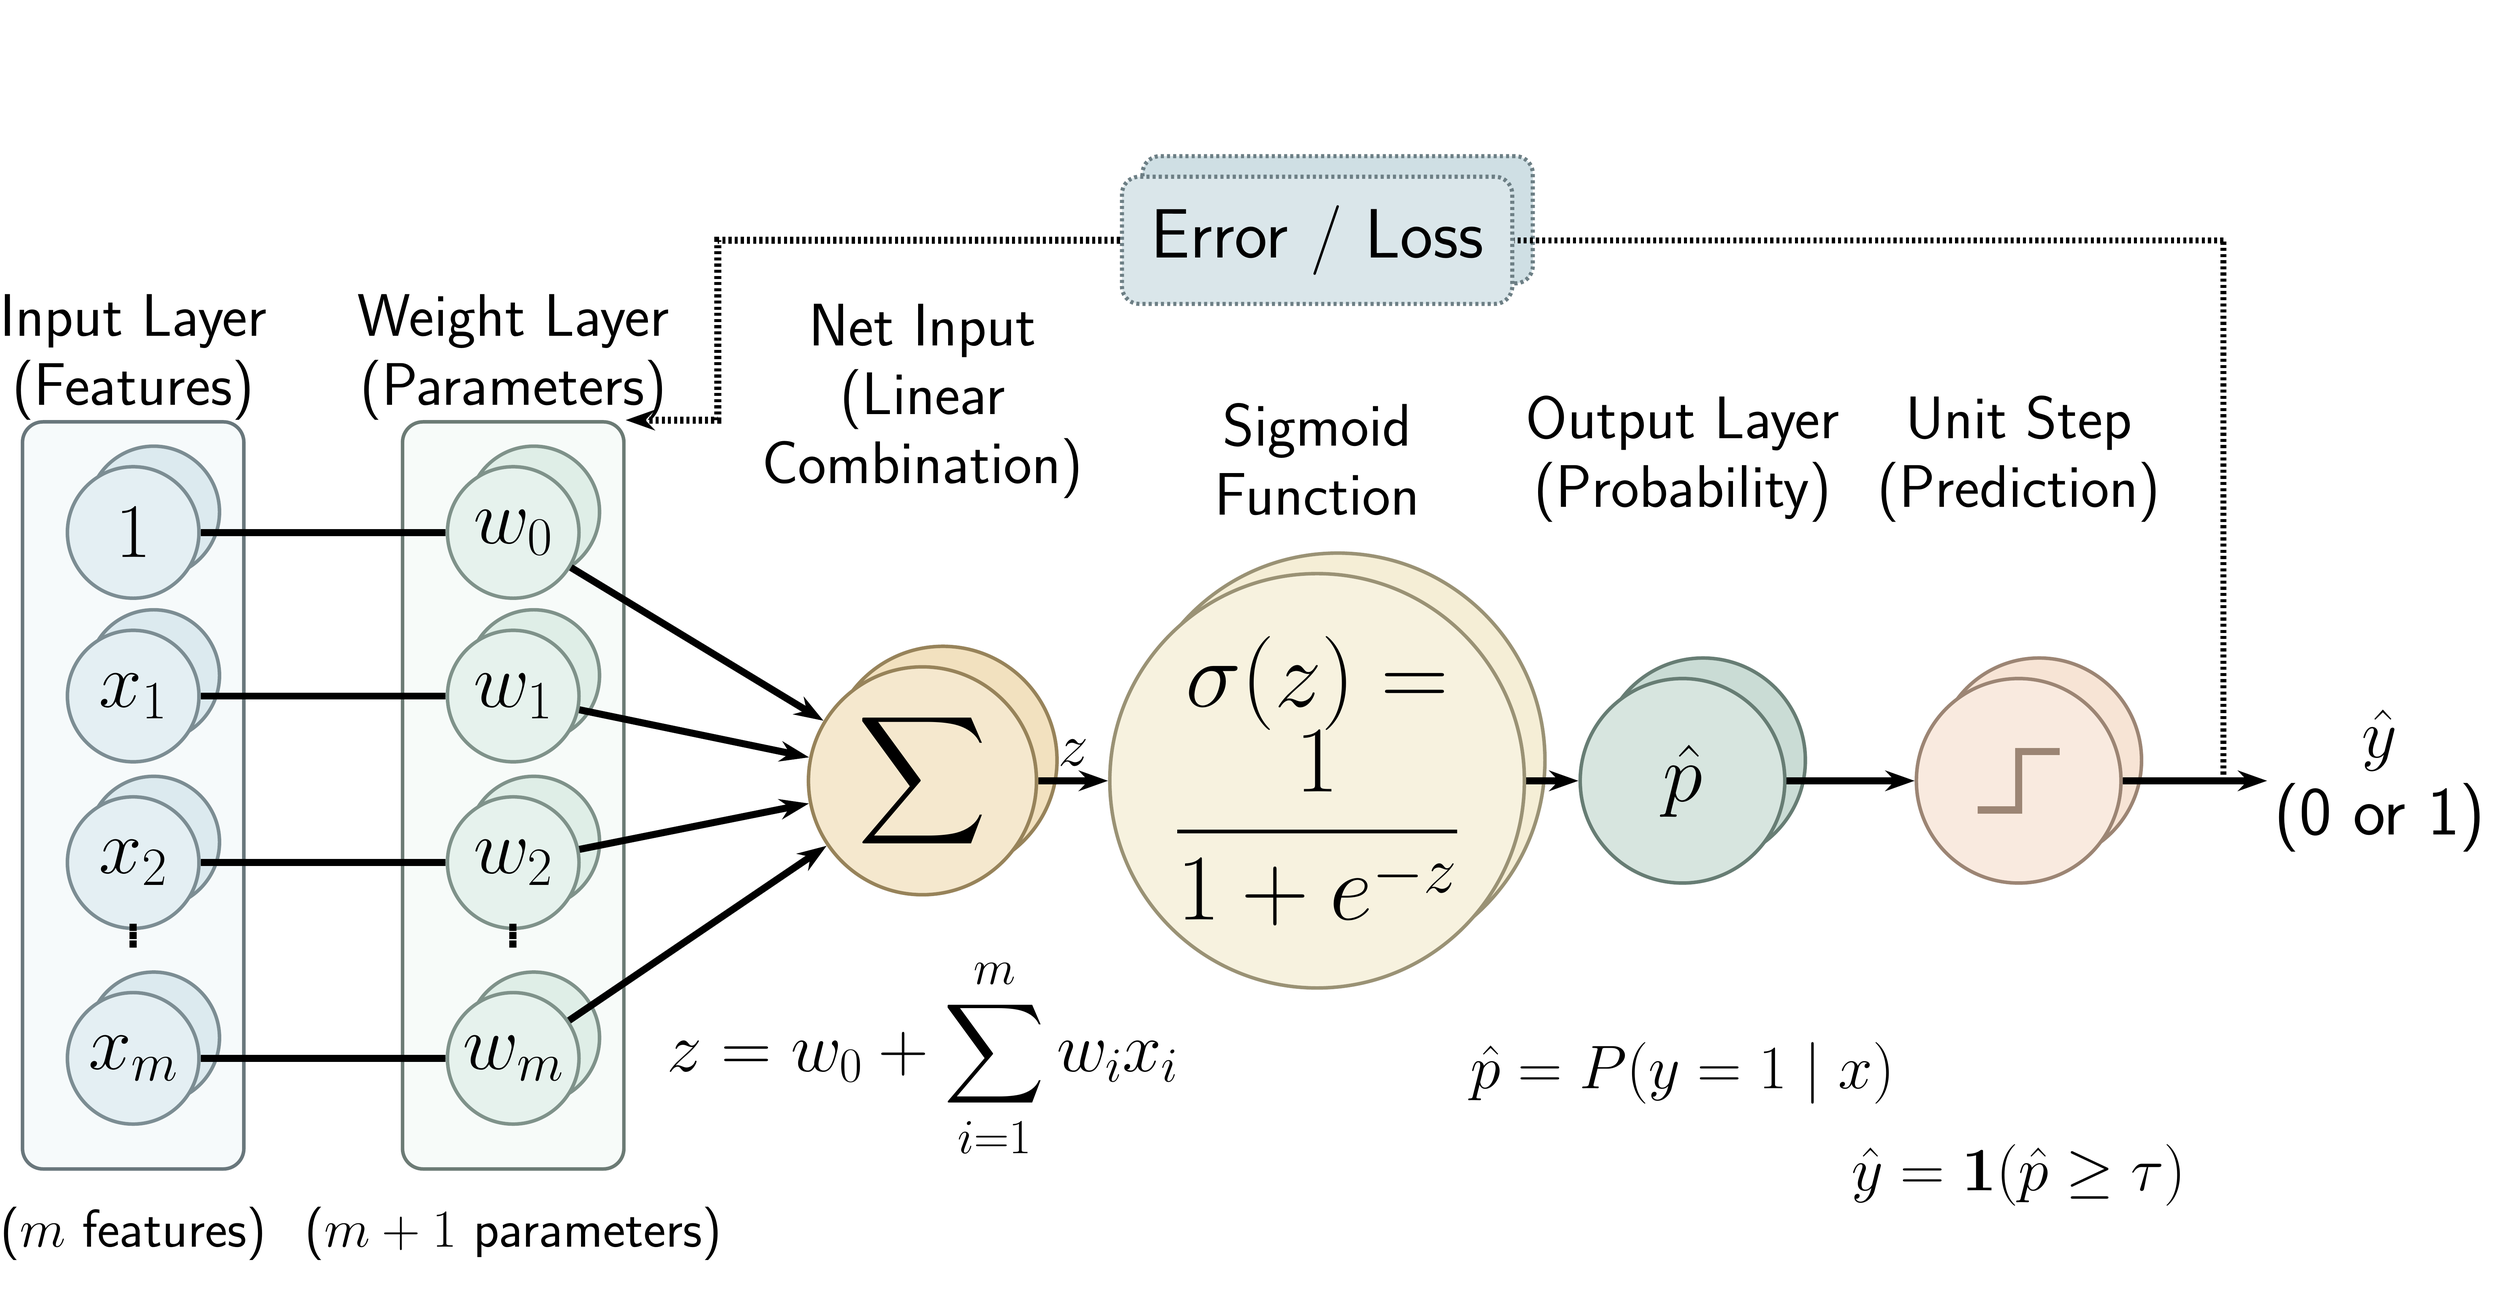
\begin{tikzpicture}[
    >=Stealth,
    font=\fontsize{75}{85.5}\selectfont\sffamily,
    text=black,
    node distance=4.2cm and 6.3cm,
    flow/.style={-{Stealth[length=10mm,width=7mm]}, line width=2.4mm, draw=black},
    plain/.style={line width=2.4mm, draw=black},
    circle3d/.style args={#1}{
        circle, draw=#1!65!black, line width=1.2mm,
        fill=#1!42!white,
        preaction={
            draw=#1!65!black, line width=1.2mm,
            fill=#1!55!white,
            transform canvas={xshift=20pt,yshift=20pt}
        }
    },
    input_node/.style={circle3d=cin, minimum size=4.5cm,
        font=\fontsize{75}{85.5}\selectfont\sffamily},
    weight_node/.style={circle3d=cexp, minimum size=4.5cm,
        font=\fontsize{75}{85.5}\selectfont\sffamily},
    sum_node/.style={circle3d=cgate, minimum size=7.8cm, align=center,
        font=\fontsize{87.5}{98}\selectfont\sffamily},
    sigmoid_node/.style={circle3d=cattn, minimum size=9.2cm, align=center,
        font=\fontsize{91.5}{102}\selectfont\sffamily},
    output_node/.style={circle3d=cout, minimum size=7.0cm, align=center,
        font=\fontsize{79}{89.5}\selectfont\sffamily},
    step_node/.style={circle3d=cpool, minimum size=7.0cm, align=center},
    label/.style={font=\fontsize{58.5}{67}\selectfont\sffamily,
        align=center, text width=12cm},
    sub/.style={font=\bfseries\fontsize{68}{68}\selectfont\sffamily, align=center},
    formula/.style={font=\fontsize{85.5}{85.5}\selectfont\sffamily,
        align=center, fill=white, draw=cgate!65!black,
        line width=1.0mm, rounded corners=5mm, inner sep=20pt},
    dots/.style={font=\fontsize{87.5}{98}\selectfont\sffamily},
    layer_box/.style args={#1}{
        fill=#1!14!white, draw=#1!55!black,
        line width=1.2mm, rounded corners=7mm, inner sep=42pt
    }
]

% Recenter: auto bbox has extra invisible margin on the left (input-side
% 3D shadow/box padding), which shifts the visible diagram off the true
% page-margin alignment after resizebox. Force a symmetric box up front
% (must come before any node/path is drawn to take effect).
% ymax extended (689.88 -> 850) to make room for the new headline title
% above the "Error / Loss" node -- xmin/xmax unchanged, so the resizebox
% width-based scale factor (and every font size) is unaffected.
\path[use as bounding box] (-204.99pt,-395pt) rectangle (2208.11525pt,850pt);

% ----------------- HEADLINE TITLE -----------------
% Bold title matching the treatment used above the random-forest.tex
% diagram; placed in the extra headroom created by the bbox extension above.


% ----------------- INPUT LAYER -----------------
\node[input_node] (x0) at (-3.0, 12.0) {$1$};
\node[input_node] (x1) at (-3.0, 6.4) {$x_1$};
\node[input_node] (x2) at (-3.0, 0.7) {$x_2$};
\node[dots] (xd) at (-3.0, -1.7) {$\vdots$};
\node[input_node] (xm) at (-3.0, -6.0) {$x_m$};

\node[label] at (-3.0, 18.0) {Input Layer\\(Features)};
\node[font=\sffamily\fontsize{52}{62}\selectfont,align=center] at (-3.0, -12.0) {($m$ features)};

% ----------------- WEIGHT LAYER -----------------
\node[weight_node] (w0) at (10.0, 12.0) {$w_0$};
\node[weight_node] (w1) at (10.0, 6.4) {$w_1$};
\node[weight_node] (w2) at (10.0, 0.7) {$w_2$};
\node[dots] (wd) at (10.0, -1.7) {$\vdots$};
\node[weight_node] (wm) at (10.0, -6.0) {$w_m$};

\node[label] at (10.0, 18.0) {Weight Layer\\(Parameters)};
\node[font=\sffamily\fontsize{52}{62}\selectfont,align=center] at (10.0, -12.0) {($m+1$ parameters)};

% ----------------- BACKGROUND BOXES -----------------
\begin{scope}[on background layer]
    \node[layer_box=cin, fit=(x0) (xm) (xd)] (input_box) {};
    \node[layer_box=cexp, fit=(w0) (wm) (wd)] (weight_box) {};
\end{scope}

% ----------------- INPUT TO WEIGHT CONNECTIONS -----------------
\draw[plain] (x0) -- (w0);
\draw[plain] (x1) -- (w1);
\draw[plain] (x2) -- (w2);
\draw[plain] (xm) -- (wm);

% ----------------- SUMMATION NODE -----------------
\node[sum_node] (sum) at (24.0, 3.5) {$\displaystyle\sum$};
\node[label] at (24.0, 16.5) {Net Input\\(Linear\\Combination)};
\node[sub] at (24.0, -6.0) {$z = w_0 + \displaystyle\sum_{i=1}^{m} w_i x_i$};

\draw[flow] (w0) -- (sum);
\draw[flow] (w1) -- (sum);
\draw[flow] (w2) -- (sum);
\draw[flow] (wm) -- (sum);

% ----------------- SIGMOID NODE -----------------
\node[sigmoid_node] (sig) at (37.5, 3.5) {$\sigma(z) =$ \\ $\dfrac{1}{1+e^{-z}}$};
\node[label] at (37.5, 14.5) {Sigmoid\\Function};

\draw[flow] (sum) -- node[above, font=\fontsize{58.5}{69}\selectfont\sffamily, yshift=8pt] {$z$} (sig);

% ----------------- OUTPUT NODE -----------------
\node[output_node] (out) at (50.0, 3.5) {$\hat{p}$};
\node[label] at (50.0, 14.5) {Output Layer\\(Probability)};
\node[font=\bfseries\sffamily\fontsize{60}{68}\selectfont,align=center] at (50.0, -6.5) {$\hat{p} = P(y=1\mid x)$};

\draw[flow] (sig) -- (out);

% ----------------- UNIT STEP NODE -----------------
\node[step_node, path picture={
    \draw[line width=2.5mm]
      (path picture bounding box.center) ++(-1.4,-1.0)
      -- ++(1.4,0) -- ++(0,2.0) -- ++(1.4,0);
}] (step) at (61.5, 3.5) {};
\node[label] at (61.5, 14.5) {Unit Step\\(Prediction)};
\node[font=\bfseries\sffamily\fontsize{60}{68}\selectfont,align=center] at (61.5, -10.0) {$\hat{y} = \mathbf{1}(\hat{p} \geq \tau)$};

\draw[flow] (out) -- (step);

% ----------------- FINAL PREDICTION -----------------
\coordinate (final_out) at (70.0, 3.5);
\draw[flow] (step) -- (final_out)
    node[right, font=\fontsize{67}{75}\selectfont\sffamily, align=center]
    {$\hat{y}$\\(0 or 1)};

% ----------------- ERROR / LOSS FEEDBACK -----------------
\node[draw=cmeta!65!black, dashed, rounded corners=6mm, line width=1.4mm,
      font=\fontsize{68}{76}\selectfont\sffamily,
      fill=cmeta!42!white, inner sep=28pt,
      preaction={
          draw=cmeta!65!black, dashed, rounded corners=6mm, line width=1.4mm,
          fill=cmeta!55!white,
          transform canvas={xshift=20pt,yshift=20pt}
      }] (loss) at (37.5, 22.0) {Error / Loss};

% Feedback loop
\coordinate (feedback_start) at (68.5, 3.5);

\draw[dashed, line width=2.0mm] (feedback_start) -- (68.5,22.0);
\draw[dashed, line width=2.0mm] (68.5,22.0) -- (loss.east);

\coordinate (feedback_turn) at (17.0,22.0);
\draw[dashed, flow] (loss.west) -- (feedback_turn) |-
    (weight_box.north east);

\end{tikzpicture}

\endgroup
\lrenddocument}
    \caption{Logistic Regression: a weighted sum of the inputs passed through a sigmoid.}
    \label{fig:logistic_regression}
\end{figure}

In the model, the features are linearized to give a score,
\begin{equation}
z = w^\top x + b,
\label{eq:logreg_score}
\end{equation}
where $w$ is the weight of the features and $b$ is a bias that changes the aggregate baseline
and the score is transformed to a probability using Equation~\eqref{eq:sigmoid}. Training is
used to minimise penalised binary cross-entropy loss,
\begin{equation}
\mathcal{L} = -\frac{1}{n}\sum_{i=1}^{n}\left[y_i \log p_i + (1-y_i)\log(1-p_i)\right] + \lambda\,R(w),
\label{eq:logreg_loss}
\end{equation}
with the first term preferring to penalise certain confident errors more than uncertain ones,
and the second term, $R(w)$, ensures that the weights are kept small in order to prevent any
single feature dominating.

Its value to the ensemble lies in that simplicity. Since it cannot represent interactions, it cannot invent
interactions, and consequently overfits much less than the tree ensembles: when the boosting
models become over-confident on a given strain the linear model remains closer to the average
and the meta-learner can learn on it.

\subsubsection{Random Forest}

Random Forest~\cite{breiman2001rf} operates in the reverse direction to boosting: a large
number of trees are constructed and averaged, not in series. Two sources of randomness ensure
that they are not duplicates of each other, a bootstrap sample of the
strains~\cite{breiman1996bagging} per tree and random selection of features to be explored at
each split, making their respective errors point in different directions and most of them
cancel. The architecture is shown in Figure~\ref{fig:random_forest_architecture}.

\begin{figure}[H]
    \centering
    \begin{adjustbox}{max width=\textwidth, max totalheight=0.60\textheight, center}
    
\newcommand{\rfdrawtree}[3]{
  \begin{scope}[shift={(#2,#3)}]
    \node[treenode] (root-#1) at (0,0) {};
    \node[treenode] (l1-#1)   at (-1.4,-1.0) {};
    \node[treenode] (r1-#1)   at (1.4,-1.0) {};
    \node[treenode] (ll1-#1)  at (-2.1,-2.0) {};
    \node[treenode] (ll2-#1)  at (-0.7,-2.0) {};
    \node[treenode] (rr1-#1)  at (0.7,-2.0) {};
    \node[treenode] (rr2-#1)  at (2.1,-2.0) {};

    \node[treenodew] (lll1-#1) at (-2.6,-3.2) {};
    \node[treenodew] (lll2-#1) at (-1.7,-3.2) {};
    \node[treenodew] (ll21-#1) at (-1.0,-3.2) {};
    \node[treenodew] (ll22-#1) at (-0.3,-3.2) {};
    \node[treenodew] (rr11-#1) at (0.3,-3.2) {};
    \node[treenodew] (rr12-#1) at (1.0,-3.2) {};
    \node[treenodew] (rr21-#1) at (1.7,-3.2) {};
    \node[treenodew] (rr22-#1) at (2.6,-3.2) {};

    \draw[line] (root-#1) -- (l1-#1);   \draw[line] (root-#1) -- (r1-#1);
    \draw[line] (l1-#1) -- (ll1-#1);    \draw[line] (l1-#1) -- (ll2-#1);
    \draw[line] (r1-#1) -- (rr1-#1);    \draw[line] (r1-#1) -- (rr2-#1);
    \draw[line] (ll1-#1) -- (lll1-#1);  \draw[line] (ll1-#1) -- (lll2-#1);
    \draw[line] (ll2-#1) -- (ll21-#1);  \draw[line] (ll2-#1) -- (ll22-#1);
    \draw[line] (rr1-#1) -- (rr11-#1);  \draw[line] (rr1-#1) -- (rr12-#1);
    \draw[line] (rr2-#1) -- (rr21-#1);  \draw[line] (rr2-#1) -- (rr22-#1);
  \end{scope}

  \draw[ar] (ds#1.south) -- (root-#1.north);

  \node[box, minimum width=5.2cm, mainfont]
    (t#1lbl) at (#2,#3-5.3) {Decision\\Tree #1};
  \draw[line] (#2,#3-3.4) -- (t#1lbl.north);
}

\begin{tikzpicture}[
    >=Stealth,
    font=\bfseries\fontsize{24}{26.5}\selectfont\sffamily,
    mainfont/.style={font=\bfseries\fontsize{24}{26.5}\selectfont\sffamily},
    titlefont/.style={font=\bfseries\fontsize{27}{29.5}\selectfont\sffamily},
    notefont/.style={font=\itshape\fontsize{19}{21}\selectfont\sffamily},
    ar/.style={-{Stealth[length=5.5mm,width=4.0mm]}, line width=1.2mm, draw=black},
    treeflow/.style={-{Stealth[length=5.5mm,width=4.0mm]}, line width=1.2mm,
        draw=black, shorten <=3pt, shorten >=3pt},
    line/.style={line width=1.2mm, draw=black},
    prism/.style args={#1}{
        rectangle, draw=#1!65!black, line width=0.5mm,
        fill=#1!42!white, align=center, minimum height=2.4cm, inner sep=18pt,
        append after command={
            \pgfextra{
                \begin{pgfonlayer}{background}
                \filldraw[fill=#1!27!white, draw=#1!65!black, line width=0.5mm]
                    (\tikzlastnode.north west) --
                    ([xshift=12pt,yshift=12pt]\tikzlastnode.north west) --
                    ([xshift=12pt,yshift=12pt]\tikzlastnode.north east) --
                    (\tikzlastnode.north east) -- cycle;
                \filldraw[fill=#1!55!white, draw=#1!65!black, line width=0.5mm]
                    (\tikzlastnode.north east) --
                    ([xshift=12pt,yshift=12pt]\tikzlastnode.north east) --
                    ([xshift=12pt,yshift=12pt]\tikzlastnode.south east) --
                    (\tikzlastnode.south east) -- cycle;
                \end{pgfonlayer}
            }
        }
    },
    box/.style={prism=cexp},
    graybox/.style={prism=cin},
    outbox/.style={prism=cgate},
    finalbox/.style={prism=cout},
    predbox/.style={rectangle, rounded corners=3mm, draw=black,
        line width=1.0mm, fill=white, minimum width=5.8cm,
        minimum height=1.8cm, align=center, mainfont},
    treenode/.style={circle, draw=black, line width=0.9mm,
        fill=cexp, fill opacity=0.85, minimum size=22pt, inner sep=0pt},
    treenodew/.style={circle, draw=black, line width=0.9mm,
        fill=cin, fill opacity=0.65, minimum size=22pt, inner sep=0pt},
    lbl/.style={notefont}
]

\node[graybox, minimum width=7.0cm, mainfont]
    (input) at (0,2.5) {Training Data};

\def\dsY{-2.8}
\node[graybox, minimum width=6.2cm, inner xsep=10pt, mainfont,
      font=\bfseries\fontsize{20}{22.5}\selectfont\sffamily] (ds1) at (-16.0,\dsY)
    {BOOTSTRAP\\SAMPLE 1};
\node[graybox, minimum width=6.2cm, inner xsep=10pt, mainfont,
      font=\bfseries\fontsize{20}{22.5}\selectfont\sffamily] (ds2) at (-5.3,\dsY)
    {BOOTSTRAP\\SAMPLE 2};
\node[graybox, minimum width=6.2cm, inner xsep=10pt, mainfont,
      font=\bfseries\fontsize{20}{22.5}\selectfont\sffamily] (dsd) at (5.3,\dsY)
    {$\boldsymbol{\cdots}$};
\node[graybox, minimum width=6.2cm, inner xsep=10pt, mainfont,
      font=\bfseries\fontsize{20}{22.5}\selectfont\sffamily] (dsN) at (16.0,\dsY)
    {BOOTSTRAP\\SAMPLE $N$};

\coordinate (sampleRail) at (0,0.0);
\draw[line] (input.south) -- (sampleRail);
\draw[line] (ds1.north |- sampleRail) -- (dsN.north |- sampleRail);
\foreach \sample in {ds1,ds2,dsd,dsN}{
    \draw[ar] (\sample.north |- sampleRail) -- (\sample.north);
}

\node[lbl, align=center, fill=white, inner sep=10pt, draw=black,
      line width=0.5mm, rounded corners=2mm] at (0,-5.5)
    {Independent trees use a random subset of features at each split};

\def\treeY{-7.0}
\rfdrawtree{1}{-16.0}{\treeY}
\rfdrawtree{2}{-5.3}{\treeY}
\node[titlefont, scale=1.6] at (5.3,\treeY-1.6) {$\cdots$};
\rfdrawtree{N}{16.0}{\treeY}
\node[titlefont, scale=1.6, text=black!55] at (5.3,\treeY-5.3) {$\cdots$};

\node[predbox] (pred1) at (-16.0,-14.8) {Prediction 1};
\node[predbox] (pred2) at (-5.3,-14.8) {Prediction 2};
\node[predbox] (predN) at (16.0,-14.8) {Prediction $N$};
\node[titlefont, scale=1.6, text=black!55] at (5.3,-14.8) {$\cdots$};

\draw[treeflow] (t1lbl.south) -- (pred1.north);
\draw[treeflow] (t2lbl.south) -- (pred2.north);
\draw[treeflow] (tNlbl.south) -- (predN.north);

\node[prism=cgate, minimum width=11.0cm, minimum height=2.6cm,
      mainfont]
    (vote) at (0,-18.8) {Combine Predictions};

\coordinate (predictionRail) at (0,-16.5);
\draw[line] (pred1.south) -- (pred1.south |- predictionRail);
\draw[line] (pred2.south) -- (pred2.south |- predictionRail);
\draw[line] (predN.south) -- (predN.south |- predictionRail);
\draw[line]
    (pred1.south |- predictionRail) -- (predN.south |- predictionRail);
\draw[ar] (predictionRail) -- (vote.north);

\node[outbox, minimum width=12.0cm, minimum height=2.8cm,
      mainfont]
    (agg) at (0,-22.5) {Majority Vote\\or Probability Average};
\draw[ar] (vote.south) -- (agg.north);

\node[finalbox, minimum width=10.5cm, minimum height=2.8cm,
      mainfont]
    (out) at (0,-26.3) {Final Prediction\\Resistant / Susceptible};
\draw[ar] (agg.south) -- (out.north);

\end{tikzpicture}
    \end{adjustbox}
    \caption{Random Forest: independent trees trained on bootstrapped samples, then averaged.}
    \label{fig:random_forest_architecture}
\end{figure}

Given a sample $x$, the predicted probability of resistance is the average of the per-tree
probability estimates:
\begin{equation}
\hat{p}(x) = \frac{1}{T} \sum_{t=1}^{T} p_t(x),
\label{eq:rf_score}
\end{equation}
where $p_t(x)$ is the proportion of the leaf in the tree $t$ that $x$ visits that is of class
one. Graded probabilities are meta-features that would not be provided by a hard majority
vote, and are required by the stacking layer.

\vspace{1em}

Random Forest adds stability instead of optimum accuracy. The predictions are relatively
robust to slight changes in the training data, which is a property that boosting models in
general do not have, and thus the ensemble will certainly possess an element that is hard to
push to one extreme.

\FloatBarrier
\subsection{Neural Lenses}

The neural feature extractor has three lenses that correspond to the three genomic views.
Each reads its respective view, creates a short representation in a 64-length summary vector
$z$, and outputs seven scores, for each antibiotic. All three struggle with the same
challenge: each strain is characterised by thousands of genes, but most of those genes
are not relevant for any one antibiotic and which ones are relevant changes with drug. This
calls for a mechanism that can focus on a handful of pertinent genes without any prior
knowledge as to which. This mechanism is the gated attention of Ilse et\
al.~\cite{ilse2018attention}, which is an extension of the attention
mechanism~\cite{vaswani2017attention} for the scenario where only a few items in a large bag
are informative. Every element $h$ is given a relevance score,
\begin{equation}
e = w^\top \big(\tanh(V h) \odot \sigma(U h)\big),
\label{eq:gated_attn}
\end{equation}
and the $U$, $V$ and $w$ are learned in training and $\odot$ represents element-wise
multiplication. The expression has two branches for a reason. The $\tanh$ branch puts forward
the degree to which this element appears to be valuable and results in a value between $-1$
and $1$. The $\sigma$ branch is a gate which generates a value in the range 0 to 1 that
determines the portion of that proposal to permit through. An element may thus be suppressed
even though it may appear on the surface to be informative which cannot be done by ordinary
attention. The scores are normalised with a softmax giving them weights which sum up to one
and the pooled summary is the weighted sum of the elements. In short, each lens becomes the sole author of the very brief write-up of a lengthy document.

\subsubsection{Motif Pattern Encoder}

The Motif Pattern Encoder reads SNP blocks, whose shape is $(G, L)$ where $G = 5{,}000$ genes
and $L = 64$ positions per gene. It is used to identify short local motifs, or patterns, of
mutations within a gene. The reasoning is that one mutation is generally silent, but then two or three mutations in
the same gene, close together in the DNA, are more likely to break or change the protein that
the gene codes for.
The natural device to this is a convolutional network, since a convolution is performed by
sliding a small window over a sequence and finding a pattern anywhere in the sequence.

Each gene has two convolutional layers stacked:
\begin{equation}
h_g = \mathrm{ReLU}\!\left(\mathrm{Conv1d}_{16 \to 32}\big(\mathrm{ReLU}(\mathrm{Conv1d}_{1 \to 16}(x_g))\big)\right),
\label{eq:expertA_conv}
\end{equation}
with windows of width three, with dropout~\cite{srivastava2014dropout} between layers. The
initial layer is trained on 16 simple patterns and the second layer is trained on 32 more
complex patterns based on the simple ones, thus, the model is constructed to be based on
simple motifs and then compound motifs. A masked max-pooling step then prunes each gene to a
fixed length vector by retaining, in each learned pattern, the strongest response it could
find anywhere in that gene. The mask makes sure that padding positions in shorter genes are
not considered as real data. The per-gene vectors are lastly pooled between genes with the
gated attention of Equation~\eqref{eq:gated_attn} to yield the representation
$z_A \in \mathbb{R}^{64}$ and per-antibiotic scores $\ell_A \in \mathbb{R}^{7}$.
Figure~\ref{fig:expertA} shows the encoder.

\begin{figure}[H]
  \centering
  \resizebox{\textwidth}{!}{\includestandalone{images/pnn_expertA}}
  \caption{Motif Pattern Encoder: a SNP block passes through two convolutional layers, masked max-pooling, and gated attention over genes.}
  \label{fig:expertA}
\end{figure}

This design is based on a direct experiment as opposed to reasoning solely. When a
convolution is done, only near positions in the input actually are related which is called
locality. We checked that this assumption is true throughout the entire pan-genome by
training a plain one-dimensional convolutional network on the full sequence of variants,
\begin{equation}
h^{(l)} = \mathrm{MaxPool}\!\left(\mathrm{ReLU}\!\left(\mathrm{BN}\!\left(\mathrm{Conv1d}_l\!\left(h^{(l-1)}\right)\right)\right)\right),
\qquad l = 1, 2, 3,
\label{eq:naive_cnn}
\end{equation}
with $h^{(0)}$ the embedded variant sequence and four convolutional layers of widths 9, 7, 5
and 3 and channel sizes 64, 96, 128 and 128 in turn, the last of which skips the pooling step
and is instead reduced by global average pooling and a single linear readout,
$\hat{\ell} = w^\top \mathrm{AvgPool}(h^{(4)}) + b$, and then randomly shuffling the order
of the variants. If position were actually meaningful, then shuffling would have hurt performance but it did
not: the model performed equally well with the shuffled input, providing further evidence that
the order of variants in the pan-genome has no signal and that a convolution at this scale is
learning nothing about position. Within a single gene this is not the case, since there the
order of sequence is biologically real. The Motif Pattern Encoder thus only uses convolution
within blocks of genes, which is precisely where the locality assumption passes the test.
Pillar 1 is this experiment, and the results are presented in Chapter~\ref{ch:results}.

\subsubsection{Gene Feature Attention Module}
\label{subsec:lensB}

The Gene Feature Attention Module reads the presence and absence profile of the genes, a
binary vector of 32{,}441 genes indicating which genes each strain has. It has been employed to
detect acquired resistance, but in a totally different manner than is required for setting up
a system to detect mutational resistance. The mechanism by which a strain can become resistant is by acquiring a
completely new gene, the original strain did not have, usually through a plasmid. This gene
is either missing or there it is; so there is no amount of mutation analysis that would find
it. The reason why this view is present is to make such a case.

It assigns each gene a learnable embedding, which is just a short vector that the model
learns that represents what that gene actually means. This embedding is only permitted to
have an effect if the gene is contained in that strain,
\begin{equation}
\tilde{e}_k = x_k \, E_k, \qquad k = 1, \dots, G_{\mathrm{pa}},
\label{eq:expertB_embed}
\end{equation}
where $E_k \in \mathbb{R}^{d_{\mathrm{token}}}$ is the learned embedding of gene $k$, and
$x_k \in \{0,1\}$ indicates whether the strain possesses gene $k$. When $x_k = 0$
$\tilde{e}_k$ is the zero vector, and therefore a missing gene cannot affect the prediction at
all regardless of what its embedding has learned. Genes that are absent in a strain are also
masked out by setting their attention scores to $-\infty$ just before the softmax of
Equation~\eqref{eq:gated_attn}, which pushes their weight to exactly zero and redundantly
provides the same conclusion.

\vspace{1em}

We cannot apply Equation~\eqref{eq:gated_attn} to $\tilde{e}_k$ directly and this is the only
point in the design we alter the mechanism, but not the data it accesses. Gated attention
scores every item based on the item representation. But for any gene the strain carries, this
representation is $\tilde{e}_k = E_k$, which is the same vector for each strain. The score
would be the same for each strain, too, the softmax would just renormalise based on which
genes that strain just happens to have, and the lens would collapse to a global gene ranking
based on presence. It was unable to convey the message that a certain gene is important to a
certain isolate, which is the whole point of laying focus here. This is not the case with the
other two lenses, as the inputs of these lenses already vary depending on the strain.

\vspace{1em}

The score is therefore dependent on the strain. For the remainder of the research, we will refer
to this as \emph{strain conditioning}. We ablate it against the standard method in
Section~\ref{subsec:attnfix}.

\begin{equation}
c = \frac{1}{\max(n_b, 1)} \sum_{k=1}^{G_{\mathrm{pa}}} \tilde{e}_k,
\qquad n_b = \sum_k x_k,
\label{eq:expertB_ctx}
\end{equation}

Here $c$ is the average embedding of the genes this strain really carries, and each gene is
scored in the company it maintains,

\begin{equation}
s_k = w^\top\Big(\tanh\big(V \tilde{e}_k + V_c\, c\big) \odot
\sigma\big(U \tilde{e}_k + U_c\, c\big)\Big),
\label{eq:expertB_score}
\end{equation}

with $V_c$ and $U_c$ being added projections. A sum of two projections is the same as a single
projection on the concatenation $[\tilde{e}_k;\, c]$, but is useful because it broadcasts $c$
rather than realising a tensor of size $B \times 32{,}441 \times 2 d_{\mathrm{token}}$, a size
that would be unaffordable at this number of genes. The additional cost is two
$d_{\mathrm{token}} \times d_{\mathrm{attn}}$ matrices. An ablation study comparing this term with the
baseline method can be found in Section~\ref{subsec:attnfix}. It increases the neural lenses by
0.035 average PR-AUC under the lineage holdout. The attention weights also modify the genes
that are being selected. The attended genes, in turn, contain 41\% as much resistance
information as the genes selected by SHAP when it is not present. They have 89\% as much
with it.

\vspace{1em}

The attention calculation is performed at single precision as opposed to half precision, as
accumulating the sum over 32{,}441 genes at reduced precision adds sufficient round-off error
to disrupt training. The attended embeddings are pooled and projected,
\begin{equation}
z_B^{\mathrm{pre}} = \sum_{k=1}^{G_{\mathrm{pa}}} a_k\, \tilde{e}_k,
\qquad
z_B = \mathrm{GELU}\!\left(W_B\, z_B^{\mathrm{pre}} + b_B\right) \in \mathbb{R}^{64},
\label{eq:expertB_out}
\end{equation}
with per-antibiotic scores $\ell_B \in \mathbb{R}^{7}$ read off $z_B$ by seven independent
linear heads, as illustrated in Figure~\ref{fig:expertB}.

\begin{figure}[H]
  \centering
  \resizebox{\textwidth}{!}{\includestandalone{images/pnn_expertB}}
  \caption{Gene Feature Attention Module: the gene presence and absence profile is embedded and pooled with masked attention over the present genes.}
  \label{fig:expertB}
\end{figure}

In a fully connected layer, each unit would require tens of thousands of weights (one per
input), and with a total of only 6{,}962 training samples, a layer that large would overfit
almost without fail. This is avoided by attention which does not increase the number of parameters as
the number of genes increases, the same small scoring function is used on each gene
separately. It also provides us with something that a dense layer does not: the weights of
attention are readable, and we can query which genes the model focused on to make a
particular prediction. The interpretability analysis of Pillar 3 is based on that readout.

\subsubsection{Cross-Antibiotic Context Module}

The Cross-Antibiotic Context Module reads the per-gene summary statistics, of shape $(G, 4)$,
where each gene is characterised (not by its complete mutation pattern) by four numbers. It
does not have the same purpose as the other two lenses: rather than deriving a new type of
signal out of the genome, it takes advantage of the interactions among the antibiotics
themselves. The rationale is biological. Drug resistance to two drugs of the same class is
normally caused by the same mechanism. If a strain develops an enzyme that can hydrolyse cefotaxime, it is likely that it will also
hydrolyse ceftazidime, as both are cephalosporins and the enzyme will act on both. In the event that we train seven absolutely independent
models, each drug must learn its own mechanism using its own labels, and the drugs that have
few resistant samples do not get enough chances to learn anything reliable. When two or more drugs within a drug class have a common representation, evidence from a
well-represented drug can assist the model with a poorly-represented drug in the same class. Figure~\ref{fig:coresistance} also puts that
argument to the test of our own data, and the answer to it is not wholly the one which the
biology predicts. That is the shared-mechanism account exactly: the two cephalosporins are by
far the most closely associated pair, at $\phi = 0.84$, and nothing else even remotely
approaches that. But below it, membership in the classes ceases to be a useful predictor.
Ampicillin is associated with trimethoprim-sulfamethoxazole at 0.55, in two unrelated classes,
about as strongly as it is with amoxicillin-clavulanate at 0.54 within its own; and ciprofloxacin,
which has no second member in the present case, is at 0.51 and 0.52 with the two
cephalosporins. Resistance genes on the same plasmid or integron travel together, regardless of whether they
target the same drug, and this group shows both patterns at once. The figure also shows why
small overlap values here cannot be used as a ranking: some antibiotic pairs are measured
against only 235 strains (amoxicillin-clavulanate and trimethoprim-sulfamethoxazole), while
others are measured against 6{,}030 (ciprofloxacin and gentamicin), so the values are not
directly comparable.

This influences the design that ensues. The cephalosporin connection would be detected by a
module that exchanged information solely inside classes (and not between them), and it would
fail to learn any cross-class link, which explains why the class-specific heads below are
initially succeeded by a refinement step that is free to learn connections not present in the
hierarchy.

\begin{figure}[htb]
  \centering
  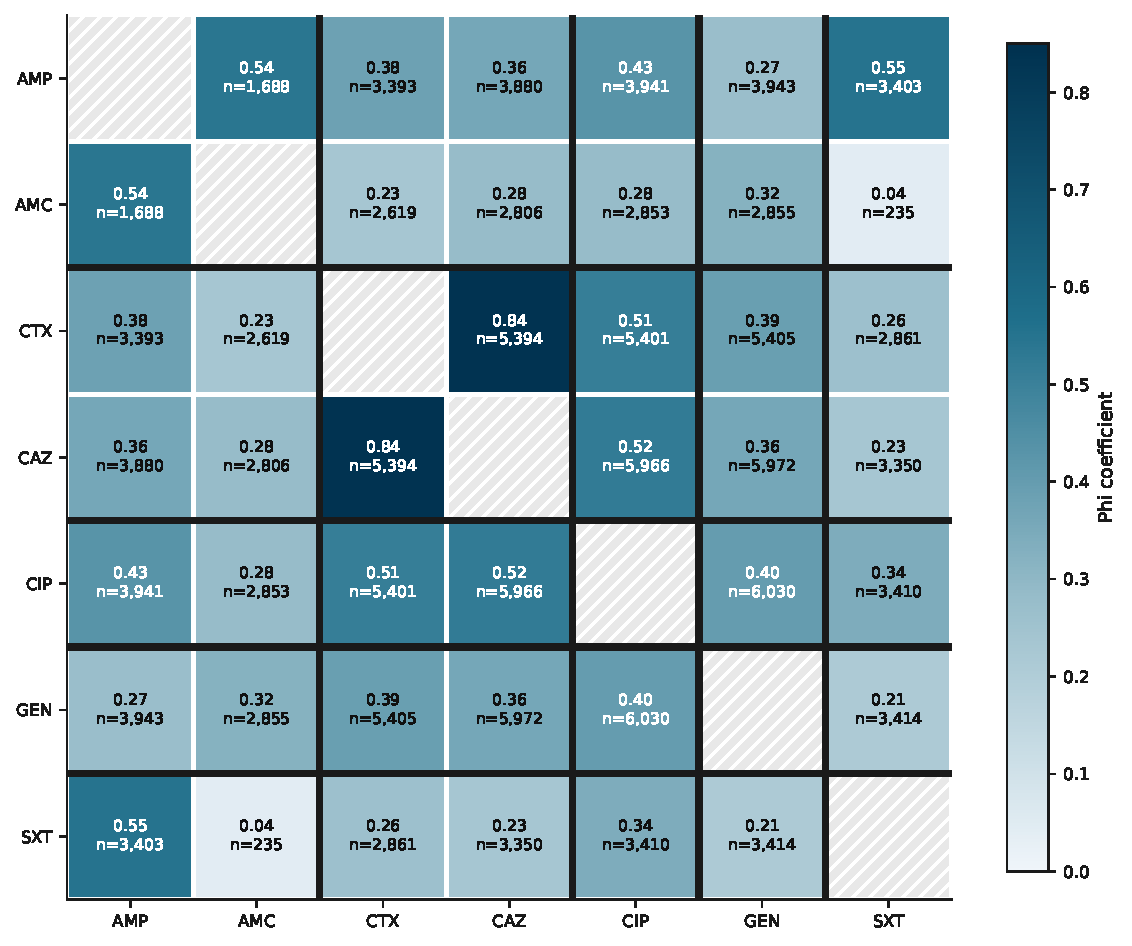
\includegraphics[width=\textwidth]{fig_coresistance.pdf}
  \caption{Pairwise co-resistance ($\phi$) between antibiotics.}
  \label{fig:coresistance}
  \fignote{Each cell is computed on the strains labelled for both drugs ($n$ shown).
  The heavy rules separate the drug classes: penicillins (AMP, AMC), cephalosporins
  (CTX, CAZ), the fluoroquinolone (CIP), the aminoglycoside (GEN) and the
  folate-pathway inhibitor (SXT). The diagonal is hatched because a drug has no
  co-resistance with itself.}
\end{figure}

This is implemented directly in the Cross-Antibiotic Context Module. Each gene's four
statistics are first transformed by a small multilayer perceptron (one per gene); then, for
global pooling across genes, gated attention is used to compute $z_C \in \mathbb{R}^{64}$.
This common representation is then decoupled into one distinct projection for each drug class;
the penicillins (AMP, AMC), the cephalosporins (CTX, CAZ), the fluoroquinolone (CIP), the
aminoglycoside (GEN), and the folate-pathway inhibitor (SXT). All of the data prior to this
split is learned jointly from all seven drugs; all of the data after this is specific to one
class,
\begin{equation}
t = \mathrm{GELU}(W_t z_C + b_t) \in \mathbb{R}^{32},
\qquad
u_g = \mathrm{GELU}(W_g t + b_g) \in \mathbb{R}^{16},
\label{eq:expertC_trunk}
\end{equation}
where $t$ is the shared trunk output and $u_g$ is the projection for drug class
$g \in \{\text{penicillin}, \text{cephalosporin}, \text{fluoroquinolone}, \text{aminoglycoside},
\text{folate}\}$. Now each antibiotic reads its initial score, according to the projection of
its own class only,
\begin{equation}
\ell^{\mathrm{init}}_{C,a} = w_a^\top u_{g(a)} + b_a,
\label{eq:expertC_ablogit}
\end{equation}
where $g(a)$ is the drug class antibiotic $a$ belongs to. Lastly, a co-resistance refinement step allows the prediction for one antibiotic to modulate
the prediction for a related one,
\begin{equation}
r = \mathrm{MLP}\!\left(\left[z_C \, ; \, \ell^{\mathrm{init}}_{C}\right]\right) \in \mathbb{R}^{7},
\qquad
\ell_C = \ell^{\mathrm{init}}_{C} + \alpha\, r,
\label{eq:expertC_cores}
\end{equation}
with $\alpha$ a learned scalar starting with a value of 0.1. This step is initialised to close
to zero, such that the model initially ignores it, and only considers it when the data
supports the step which ensures that a spurious relationship between two drugs is not baked
in at the beginning. Figure~\ref{fig:expertC} shows that $\ell_C$ is produced by the lens in
$\mathbb{R}^{7}$.

\begin{figure}[H]
  \centering
  \resizebox{\textwidth}{!}{\includestandalone{images/pnn_expertC}}
  \caption{Cross-Antibiotic Context Module: per-gene statistics are transformed, pooled with attention, and passed through drug-class heads with co-resistance refinement.}
  \label{fig:expertC}
\end{figure}

It is easier to train seven separate models and this is how we started. The issue is the lack
of balance in drugs. The number of resistant strains of gentamicin is low compared to
ampicillin and therefore there is nothing much to learn by a gentamicin-only model. There is a common base shared across all antibiotics. This base learns from the labels of
every drug, not just one. This is exactly what multi-task learning is designed to do.
Nonetheless, if the common base acquires a misleading pattern, it influences all drugs. To
limit this problem, there is a branch for each drug. Some of those mistakes can still be
corrected by these branches.

\FloatBarrier
\subsection{Mixture-of-Experts Gating and Representation Fusion}
\label{subsec:moegate}

When each of three lenses has made an opinion about each of the seven antibiotics, their
opinions will not necessarily be consistent, and here the question is to what to do with
them. The easiest would be to average the three. We discarded that, since averaging supposes
that all the three lenses will be equally useful, and they are not. When the resistance of a
drug is due to an acquired plasmid gene, the Gene Feature Attention Module should prevail and
the Motif Pattern Encoder can do practically nothing with it. In the case of a drug whose
resistance is due to a point mutation in a target enzyme, the opposite holds true. A decision based on the
average would drown out the voice of a stronger lens (and its view) with two weaker ones.

The mixture-of-experts gate~\cite{jacobs1991moe, shazeer2017moe} addresses this by learning
weights, rather than fixing them, and by learning them individually, one strain at a time, and
each antibiotic at a time. The three representations are combined into a single vector
$z = [z_A; z_B; z_C] \in \mathbb{R}^{192}$ and fed through a small network and softmax to
obtain
\begin{equation}
g = \mathrm{softmax}\big(\mathrm{MLP}([z_A; z_B; z_C])\big), \qquad g \in \mathbb{R}^{B \times 7 \times 3},
\label{eq:moe_gate}
\end{equation}
so that for each antibiotic, the three weights are non-negative and sum to one. The fused
score of antibiotic $a$ is then the gate-weighted sum of the lens scores,
\begin{equation}
\ell^{\mathrm{fin}}_{a} = \sum_{e=1}^{3} g_{a,e}\,\ell_{e,a},
\qquad
p^{\mathrm{neu}}_{a} = \sigma\!\left(\ell^{\mathrm{fin}}_{a}\right).
\label{eq:fusion}
\end{equation}

One common failure mode of a gate of this type is often referred to in the literature on
mixture-of-experts as expert collapse, and is known here as gate collapse. It is often the
case that in the early stages of training, one of the lenses is a bit better than the rest, by
chance. This slight edge is noticed by the gate and makes it transfer more weight onto that
lens. The larger the gradient, the more weight. This means that the lens will learn quicker and
even more from the gate. After a few epochs the other two
lenses have ceased to be trained at all and the model silently transforms into a single-lens
network. To avoid this we count the spread out of the gate with each antibiotic $a$ by its
Shannon entropy,
\begin{equation}
H(g_a) = -\sum_{e=1}^{3} g_{a,e} \log g_{a,e},
\label{eq:gate_entropy}
\end{equation}
which is largest when the three weights $g_{a,e}$ are equal and smallest when the gate has
collapsed onto a single lens. Then we introduce an entropy term into the loss, $-\beta$ times
the mean of $H(g_a)$ over antibiotics,
\begin{equation}
\mathcal{L}_{\mathrm{ent}} = \beta \sum g \log g,
\label{eq:entropy_reg}
\end{equation}
that is minimized with a gate that spreads its weight and maximized with a gate that
concentrates its weight on one lens. With a small weight $\beta$ this pushes the gate to keep
all three lenses active whilst leaving it free to favour one where the evidence actually
supports it. We track the average weight assigned to each lens during training, and
automatically increase the entropy weight when any lens's weight goes below a threshold. The
gating and fusion step is shown in Figure~\ref{fig:moegate}.

\begin{figure}[H]
  \centering
  \resizebox{\textwidth}{!}{\includestandalone{images/pnn_moegate}}
  \caption{Mixture-of-experts gating and fusion: the gate produces per-antibiotic weights over the three lens representations.}
  \label{fig:moegate}
\end{figure}

\FloatBarrier
\subsection{Stacking Meta-Learner}
\label{subsec:metalearner}

The decision is eventually made by a logistic-regression meta-learner which combines the
neural probability with the five classical out of fold probabilities. This is stacked
generalisation in the sense of Wolpert~\cite{wolpert1992stacked}, where the predictions of
multiple base learners are used as features for a second-level model. Unlike simple
averaging, the weighting is not fixed in advance; the six probabilities are treated as inputs
to a tiny model that learns from the data how much to trust each of them. That is the
difference between consulting six specialists and taking the mean of their replies, and
consulting six specialists whose respective track records have been studied with a view to
determining which of them is apt to be right in which class of case.

The meta-learner constructs the feature vector $\phi_a$ of each antibiotic $a$,
\begin{equation}
\phi_a = \left[\,p^{\mathrm{neu}}_a,\; p^{(1)}_a,\; p^{(2)}_a,\; p^{(3)}_a,\; p^{(4)}_a,\; p^{(5)}_a\,\right],
\label{eq:meta_features}
\end{equation}
where $p^{(m)}_a$ are the probabilities of the five base learners, and calculates
\begin{equation}
\eta_a = w_a^\top \phi_a + b_a,
\qquad
\hat{p}_a = \sigma(\eta_a),
\label{eq:meta_logit}
\end{equation}
for each antibiotic, using an L2-penalised logistic regression with $C = 1.0$. It is a conscious decision to train one meta-learner per antibiotic: the drugs are supposed to
rely on different models, and having a common meta-learner would push all seven to make one
trade-off. The final call is obtained by thresholding the probability,
\begin{equation}
\hat{y}_a = \mathbf{1}\!\left[\hat{p}_a > 0.5\right],
\label{eq:decision}
\end{equation}
with a fixed decision threshold of 0.5. We predict all seven antibiotics jointly, so one
forward pass through the model gives a full multi-label resistance profile, which we
summarise in Figure~\ref{fig:stacking}.

\begin{figure}[H]
  \centering
  \resizebox{\textwidth}{!}{\includestandalone{images/pnn_stacking}}
  \caption{Stacking meta-learner: the neural probability and five classical out-of-fold probabilities are combined per antibiotic, then thresholded into a call.}
  \label{fig:stacking}
\end{figure}

We also tested a neural meta-learner. It is a more complex combination of the six base
predictions. The first step uses a small feed-forward layer to generate one token per
antibiotic. Subsequently, a four-head self-attention layer allows the seven tokens to exchange
information. Then, the final score of each drug is provided by a separate decoding head. This
was aimed at capturing co-resistance profiles, including the cefotaxime-ceftazidime
relationship. This drug-to-drug relationship cannot be learnt by a separate linear model. The
neural model, however, did not fare well. It scored 0.825 against the simple meta-learner's
0.849. It was not the number of input features that was the problem. The neural embedding is
folded into the meta-feature vector, bringing it to 170 dimensions. Nevertheless, there are
only about 5{,}000 strains behind those numbers. The model is further complicated by the
attention layer and seven decoding heads. Consequently, it can easily fit noise in such a
small dataset. We can directly read the weights of the linear meta-learner, letting us see
more explicitly than a deeper meta-learner might allow how the final decision broke down in
terms of how much to trust the neural arm and how much to trust each classical model for every
antibiotic.

\FloatBarrier
\subsection{Summary of Design Decisions}

Table~\ref{tab:designchoices} wraps up the primary design decisions defined in this section
along with the alternative that was considered and cause of the selection. In cases wherein a
decision was determined by measurement, not by argument, the numbers in support of the
decision are given in Chapter~\ref{ch:results}.

{\small\setlength{\tabcolsep}{5pt}
\begin{longtable}{|>{\raggedright\arraybackslash}p{2.9cm}|>{\raggedright\arraybackslash}p{3.1cm}|>{\raggedright\arraybackslash}p{7.5cm}|}
\caption{Summary of the main design decisions and the alternatives considered.}
\label{tab:designchoices}\\
\hline
\textbf{Decision} & \textbf{Alternative considered} & \textbf{Reason for the choice} \\
\hline
\endfirsthead
\hline
\textbf{Decision} & \textbf{Alternative considered} & \textbf{Reason for the choice} \\
\hline
\endhead
\hline
\multicolumn{3}{r}{\footnotesize\textit{Continued on the next page}}\\
\endfoot
\hline
\endlastfoot
Hybrid neural and classical design & A single end-to-end neural network &
With 6{,}962 samples against hundreds of thousands of features, a large network memorises
rather than generalises. Gradient boosting is far more stable in this setting, and the neural
arm supplies the interactions boosting cannot express. \\ \hline
Three genomic views & One combined feature matrix &
Mutation based and gene presence based resistance are different mechanisms, and a single
representation captures one at the cost of the other. \\ \hline
Convolution inside gene blocks & Convolution across the whole pan-genome &
A shuffle test showed that variant ordering across the pan-genome carries no information, so
convolution is only meaningful within a gene, where sequence order is real. \\ \hline
Attention over the gene profile & A dense layer over 32{,}441 genes &
A dense layer would need tens of thousands of weights and would overfit immediately.
Attention keeps the parameter count fixed and produces readable weights. \\ \hline
Shared trunk across antibiotics & Seven independent models &
Groups of antibiotics within a class may have similar resistance mechanisms, so using one
shared network allows drugs with more data to help drugs with less data. \\ \hline
Learned gate & Fixed average of the lenses &
Different antibiotics rely on different lenses, and a fixed average would dilute the
strongest opinion with two weaker ones. \\ \hline
Entropy regularisation on the gate & No regularisation &
Without it the gate collapses onto one lens early in training and the other two stop
learning. \\ \hline
Five classical base learners & One strong classical model &
Ensembles gain from disagreement. The five were chosen to span linear and non-linear, high
and low variance, and fine and coarse feature views. \\ \hline
Out-of-fold predictions & Predictions on the training data &
Training-set predictions look better than they are, which would make the meta-learner trust
the wrong models. \\ \hline
Logistic regression meta-learner & A deeper neural meta-learner &
The signal available at this layer is six base probabilities per antibiotic; the deeper
version widens that to a 170-dimensional vector but has only about 5{,}000 training rows
behind it, and its weights would not be readable. It also scored lower. \\ \hline
Gene level features & Principal component features &
Principal components mix genes together and cannot be named, which removes any possibility
of interpretation, and they scored lower. \\ \hline
\end{longtable}}



\FloatBarrier
\section{Data Collection and Preprocessing}
\label{sec:data}

All findings in this research are based on the construction of the data, and this section
explains the sources of the genomes, how raw variant files were converted to a format readable
by a model, and what was lost during the conversion. We rely on the \textit{Escherichia coli}
genotype and phenotype resource published by Arcadia Science, which has over seven thousand
strains, all of which were sampled all around the world, and have been lab-tested in terms of
their resistance.

\vspace{1em}

This resource has been published in two parts; we use both. The first
release~\cite{morin2024ecoli} was a variant calling of the collection against a pan-genome
reference and the variant files were released together with the phenotype table and strain
metadata. The second release~\cite{york2025amr} included gene presence and absence data for
all of the genes in all of the strains, as PLINK binary files. For credit and clarity, we state which view is from which release and calculate our SNP views
from the first and our gene presence view from the second, not presenting the combined result
as if it came from a single source. There are three reasons we chose this
as a resource rather than building our own collection. The variant calls were initially
quality controlled by the authoring group, effectively eliminating a significant source of
variation between studies. It is part of a pan-genome and not a single genome, so accessory
genes are part of the reference and in \textit{E. coli} many resistance genes are carried on
genes that the strain has obtained from other sources. And because another group has also
published their own analysis of the exact same strains, we can compare results between ours
and theirs later on in Chapter~\ref{ch:results}.

\vspace{1em}

The collection size varies depending on the file you are viewing: the strain metadata table
contains 6,985 rows, the phenotype matrix contains 6,983, and the presence and absence release
lists 7,043 samples. We made no effort to harmonize these, but retained only the strains which
seem everywhere necessary, as described below.

\vspace{1em}

We created a data pipeline from the raw variant files, filtering by missingness and frequency,
encoding the variants as binary columns in a data matrix, then appended this to the phenotype
table to get a matrix of 6,962 strains by 80,984 features before settling on this data. We
changed direction due to two problems. Our filters were very crude, based on arbitrary cutoffs
that had no biological significance. More seriously, the features were not structured
gene-level: each variant was simply a column, and there was no connection to the gene it was a
part of, and the entire concept of our proposed model is that mutations within the same gene
should be read jointly. For this reason, we have decided to adopt the curated release above
and rely on it from here on. The complete story of that change is provided in
Section~\ref{sec:designadj}.

\FloatBarrier
\subsection{Data Cleaning}

This primarily referred to record matching between files and encoding text phenotypes as
numbers. The genomes themselves needed no cleaning, since the variant calling had already been
done and checked.

\subsubsection{Matching Strains Across Files}

Three files were required to match for a strain to be used. The variant file is indexed by
sequencing accession. These are identified in the phenotype file by genome name. They are
mapped via a separate mapping file. An accession was kept if it was found in the variant file,
the mapping file provided a genome name, and that genome name appeared in the phenotype table.
Following this, 6,962 strains remained and these strains were used for all experiments in this
research. We also incorporated the strain metadata table, 6,821 of which (98.0 percent) matched.
Since the metadata is only utilized to work out lineage, the ones without it are not lost, they
just fall outside of a lineage group.

\subsubsection{Turning Phenotypes into Labels}

When a test is performed, the result is recorded in the phenotype file as resistant,
intermediate or susceptible and a blank is indicated where no test was performed. This was
transformed to a binary label with 1 for resistant and 0 for susceptible. In order for our
labels to be comparable with the ones produced by the group that published the dataset, we
encoded intermediate results as resistant, following the same convention as they initially
used. There is also a clinical argument for it: an intermediate result implies that the normal
dose will be insufficient, hence it is safer to call it resistant. One possible consequence of
these early steps is worth remarking on: this step leaves no intermediate category, which is
the reason that categorical agreement collapses to plain accuracy in
Section~\ref{sec:perfeval}.

\subsubsection{Handling Untested Strains}

Not all strains were tested against all drugs, and the number of drugs tested varies a great
deal from strain to strain. So,
instead of discarding incomplete lines or inserting guesses, we retained a boolean mask with
shape $6{,}962 \times 7$ that indicates which entries are real. Training loss and all
evaluation metrics are calculated only for the observed entries. Nothing is imputed anywhere
in this research. Table~\ref{tab:labels} displays what remained for us once the mask was
applied, drug by drug.

\begin{table}[htb]
\centering
\caption{The seven antibiotic labels after cleaning. Coverage is the share of the
6,962 strains tested against that drug; prevalence is the share of those that were
resistant.}
\label{tab:labels}
\small
\setlength{\tabcolsep}{3pt}
\begin{tabular}{|l|r|r|r|r|r|r|}
\hline
\textbf{Antibiotic} & \textbf{Resistant} & \textbf{Susceptible} & \textbf{Not tested} & \textbf{Tested} & \textbf{Coverage} & \textbf{Prevalence} \\
\hline
AMP & 2,439 & 2,429 & 2,094 & 4,868 & 69.9\% & \textbf{0.501} \\ \hline
CIP & 1,377 & 4,656 &   929 & 6,033 & 86.7\% & 0.228 \\ \hline
AMC & 1,180 & 2,598 & 3,184 & 3,778 & 54.3\% & 0.312 \\ \hline
SXT & 1,060 & 2,358 & 3,544 & 3,418 & \textbf{49.1\%} & 0.310 \\ \hline
GEN &   710 & 5,327 &   925 & 6,037 & 86.7\% & \textbf{0.118} \\ \hline
CTX &   823 & 4,586 & 1,553 & 5,409 & 77.7\% & 0.152 \\ \hline
CAZ &   780 & 5,193 &   989 & 5,973 & 85.8\% & 0.131 \\ \hline
\end{tabular}
\vspace{0.4em}

\noindent\footnotesize\textit{Note:} Trimethoprim-sulfamethoxazole has the lowest coverage of
the seven drugs at 49.1\%, and prevalence ranges from 0.501 for ampicillin down to 0.118 for
gentamicin, the two spreads the next paragraph discusses.
\end{table}

There are two items in this table that represent a lot of what happens later. Overall, almost
a twofold variation exists in coverage. Ciprofloxacin and gentamicin were tested for almost 87
percent of strains, but trimethoprim with sulfamethoxazole for only 49 percent, and fewer
strains tested means fewer samples behind a score, which equals a wider confidence interval.
It is the chief cause of some of our intervals in Chapter~\ref{ch:results} being so much wider
than others.

\vspace{1em}

Prevalence ranges more widely: from 0.501 for ampicillin, down to 0.118 for gentamicin. This
is important because the no-skill value of precision recall AUC is the prevalence: a score of
0.70 on gentamicin, where only 12 percent of strains resist, is a much larger gain over chance
than the same score would be on ampicillin, and we will return to this point in
Section~\ref{sec:perfeval} when comparing antibiotics. Four other antibiotics were present in
the phenotype file but dropped. They either were too small to be tested or were so biased that
a model would score well by making too many predictions to one class. The seven we kept cover
five classes of drugs, as per the requirements in FR3.

\FloatBarrier
\subsection{Data Transformation}

\subsubsection{From Variant Calls to a SNP Matrix}

The variant calls and the gene presence and absence profiles are released in two different
deposits. As a result, the first and second views below are generated from different source
files, instead of one source file. The size of the variant file is approximately 1.1 gigabytes
in compressed VCF. We streamed it
just once, and only retained a variant if two requirements were met. This had to be a
single-nucleotide change, so insertions and deletions were omitted. In addition, it had to
have a minor allele frequency of at least one percent across the collection. What this left is
recorded in Table~\ref{tab:variants}.

\begin{table}[htb]
\centering
\caption{Variant filtering during construction of the SNP matrix.}
\label{tab:variants}
\small
\begin{tabular}{|l|r|}
\hline
\textbf{Stage} & \textbf{Variants} \\
\hline
Streamed from the variant file & 2,451,184 \\ \hline
Removed: insertion or deletion &    43,799 \\ \hline
Removed: minor allele frequency below 1\% & 1,871,946 \\ \hline
\hline
\textbf{Kept} & \textbf{535,439} \\ \hline
\end{tabular}
\vspace{0.4em}

\noindent\footnotesize\textit{Note:} The 535,439 kept variants are 21.8\% of the 2,451,184
streamed from the variant file, and this
is the set that feeds every later step.
\end{table}

The team that constructed this data set reported approximately 2.4 million variants, and we
read 2,451,184, so we knew we were reading it correctly before building anything on top of it.
When the frequency filter was applied alone, 76\% of the variants were removed, with the
majority of them present in just two or three strains. If a pattern is found in so few strains,
then it cannot be expected that it will hold true for a new strain. So removing these variants
was very cheap for the model.

Genotypes are represented by small integers: 0 is the reference allele, 1, 2 or 3 are the
first, second or third alternate. Overall, 83.3 percent of the call types in the data are
reference calls and 16.3 percent are first alternate; 2.5 percent are second or third
alternate, among non-reference calls. We pass these through as integers and not in separate
columns. If the alleles are treated as integers, then allele 3 is further away from the
reference than allele 1. There is no biological basis to this. Second and third alternate
alleles are, however, only 2.5\% of non-reference calls, about one in forty. One-hot encoding
them as separate columns was therefore not worth the added complexity.

For genotypes missing, they were set to the reference allele in line with the original authors
so that our features match theirs. This is not a neutral choice: a genotype that failed to
call is assumed to match the reference and coverage is typically lower on plasmids and other
mobile elements that are less able to assemble from the short reads, which is where acquired
resistance genes typically reside. This is revisited in Section~\ref{sec:discussion}, and thus
forms part of our explanation as to why gentamicin is the hardest of the seven drugs to model.
The result is a matrix of $6{,}962 \times 535{,}439$ stored as 8-bit integers, 3.73 gigabytes,
which took about two and a half hours to build on a single consumer GPU.

\subsubsection{The Gene Presence and Absence Matrix}

Release 2 provides the presence of genes in 32,441 pan-genome loci in PLINK binary format. It
took one decision that wasn't necessarily obvious to make these into a usable matrix. The
numbers stored are 0 and 2. Nothing in the release specifies which one means the gene is
present and the two readings have opposing biology, so we tried both against something we
could test. If non-zero is considered present, then it gives a median gene prevalence of
0.966, which is about 28,700 genes in an average strain. A median prevalence of 0.034 and an
average of 3,727 genes per strain (range 2,141 to 8,333) was obtained when zero was coded as
present. An \textit{E. coli} genome contains about 4-5 thousand genes, limiting the reading to
the second one, which is the one we use.

\vspace{1em}

We register this check because the incorrect option need not have thrown any error. The model
would have learned as usual with its gene matrix inverted and since this view has a lot of
weight in our final model, everything further down it would have been incorrect in a
non-obvious way. The per-strain gene count is a sanity check and is now done automatically on
every new matrix build. There are 6,962 strains of which 6,949 are found in the PLINK sample
list. The other 13 (0.19 percent) do not have a record of gene presence. In the default policy
of the pipeline these rows are not dropped or masked, instead remaining as an all-zero
gene-presence vector, meaning that Lens B interprets them as a strain with non-detected genes
instead of excising them from the dataset.

\subsubsection{Per-Gene Statistics}

The third view summarises each gene with four values calculated from its SNPs: mean value of
the alleles, variance of the alleles, number of positions that do not match the reference, and
maximum value of the alleles. It is a very broad perspective, and it cannot tell where a
mutation is occurring in a gene. It does offer stability and compactness though. It also
provides a brief and reliable gene-level view of variation which complements the other two
views.

Each of these four statistics is on a different scale. Therefore, each one is adjusted in
order to have zero mean and unit variance before it gets to the third lens. Only the training
partition is used to calculate the means and standard deviations. They are then applied
unchanged to the validation and test partitions. This means that no test genome impacts the
scaling.

\subsubsection{Lineage Encoding}

Bacterial populations are structured in lineages and strains within a lineage are likely to
share their genetic background and resistance pattern. In order to determine if our model was
using lineage or mechanism we first had to determine the lineage of each strain, which the
data set did not explicitly give us, but we worked it out ourselves. The phylogroup was not provided directly. We have developed it in two steps. An
explicit phylogroup assignment, if any, is taken from the typing field in the strain metadata.
In the absence of such information, the multi-locus sequence type and mapping to a phylogroup
were done with the help of a look-up table of 57 common multi-locus sequence types. There is no
record of the origin of this particular table in the original notebooks used for data
preparation. No citation or generation script is recorded with it and it is reported here as an
undocumented lookup, not as a part of a published scheme. If a strain is found that cannot be
fixed by either route it is marked Unknown.
Table~\ref{tab:phylogroups} gives the result.

\begin{table}[htb]
\centering
\caption{Phylogroup composition of the 6,962 strains.}
\label{tab:phylogroups}
\small
\begin{tabular}{|l|r|r|}
\hline
\textbf{Phylogroup} & \textbf{Strains} & \textbf{Share} \\
\hline
B2      & 3,542 & \textbf{50.9\%} \\ \hline
Unknown & 1,697 & \textbf{24.4\%} \\ \hline
D       &   723 & 10.4\% \\ \hline
A       &   317 &  4.6\% \\ \hline
F       &   307 &  4.4\% \\ \hline
B1      &   258 &  3.7\% \\ \hline
C       &   114 &  1.6\% \\ \hline
E       & \textbf{4} &  0.1\% \\ \hline
\end{tabular}
\vspace{0.4em}

\noindent\footnotesize\textit{Note:} B2 alone is 50.9\% of the collection, 24.4\% of strains
have no assigned phylogroup, and phylogroup E has only 4 members, too few for any per-group
estimate; these are the three limits the next paragraph discusses.
\end{table}

There are, however, three features of this table which restrict what can be read from it; we
should like to mention them here rather than have them pointed out later. B2 is slightly more
than half the collection, so the analysis of splitting the collection by phylogroup is a
majority analysis of B2 vs.\ the remainder of the collection. There is little use for a
per-group estimate of the diversity of the Unknown group because almost a quarter of strains
could not be assigned to any group, and phylogroup E has a small number of members (four),
which is too small to make any estimate meaningful. For this reason we consider the phylogroup
as a broad category and not anything else. It is encoded as an eight-way one-hot vector and
used as a covariate and as a grouping variable. We do not consider it as a fine description of
ancestry, and Section~\ref{sec:discussion} demonstrates why this distinction is relevant.
Figure~\ref{fig:phylogroup_composition} shows how uneven the composition is.

\begin{figure}[htb]
\centering
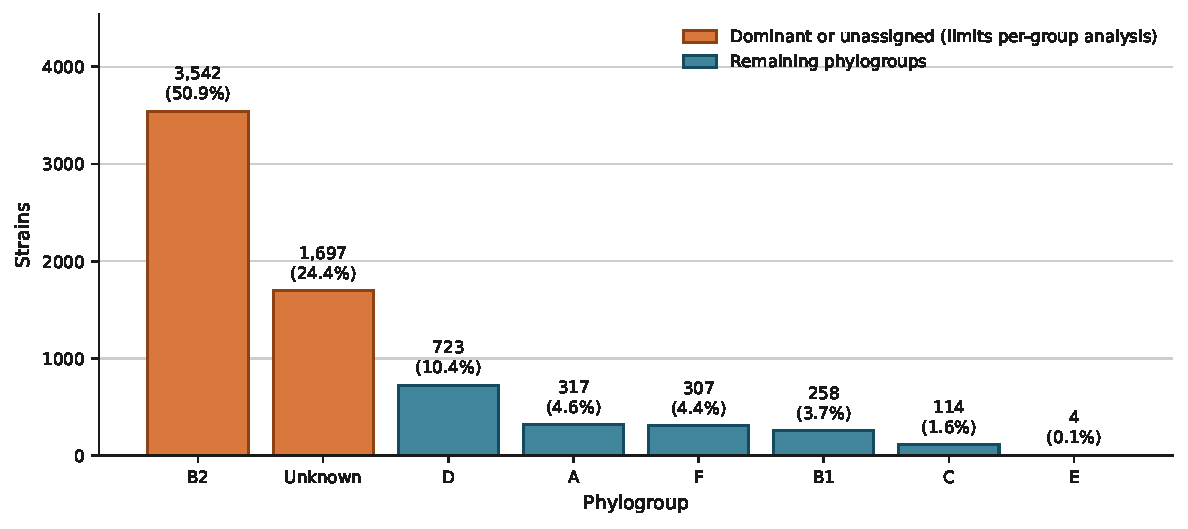
\includegraphics[width=0.94\textwidth]{fig_population_structure.pdf}
\caption{Phylogroup composition of the 6{,}962 strains.}
\label{fig:phylogroup_composition}
\fignote{The values of Table~\ref{tab:phylogroups} drawn to scale: a split by
phylogroup is largely a split of B2 against everything else.}
\end{figure}

\FloatBarrier
\subsection{Data Integration}

We had two checks before training. The three feature matrices were of different files. They
were also produced in various stages. We therefore made sure that they had the same strains in
the same order. We also verified that they were using the same names of genes. The first confirmed that the ordering of all 6,962 strain identifiers is
identical in all views; otherwise, one genome's SNPs would be paired with another genome's
genes.

\vspace{1em}

The latter one discovered a real challenge. None of the genes were found in common when the
gene identifiers in the SNP views were compared to the presence and absence view, because the
PLINK reader had created its own placeholder names for the genes and not read the actual gene
identifiers from the annotation file. Once the reader was corrected, all 5,000 genes chosen for
the SNP views were found in the 32,441-gene catalogue, a 100 per cent overlap. Nothing would have
failed visibly had this check not been run. The model would have received views labelled with the
wrong gene names, and the gene-level reading from Section~\ref{subsec:attnfix} would have been
comparing labels with no meaning against one another. Both the checks are now programmed as a
fixed step prior to any training run.

\FloatBarrier
\subsection{Data Reduction}

There are 535,439 features for 6,962 strains (some 77 candidate features for each sample). So,
it was not an optimisation to reduce the feature space. It was necessary for modelling, for the
reason explained in Section~\ref{subsec:hybrid}. The features were reduced at the gene level
rather than at the individual-variant level as the model operates at the gene level. Lastly,
only the genes that survived the two filters were retained. If a gene has fewer variable
positions, we cannot support a within-gene pattern, which is what our first view is designed to
find; thus the variability filter retains a gene if it has five or more SNPs across the
collection. After this step, 13,799 of the 18,975 genes in the matrix remain. These genes are
then sorted by importance in the gradient boosting model~\cite{chen2016xgboost} using the
importance filter. That model is trained separately for each of the seven antibiotics.
First, we filtered each set of SNPs with a chi-squared pre-filter and kept the top 50,000 per
drug, and trained a single XGBoost model for each antibiotic on its respective chi-squared
filtered subset, calculating each gene's cumulative gain for each model. The final importance
score for each gene is the sum of the per-antibiotic importance over all seven models, and the
5,000 most important (highest summed) genes are retained.

\vspace{1em}

The two filters were fitted solely based on the training partition. This is quite easy to
forget, and quite hard to do well: had the test labels been visible during ranking, they would
have changed what features exist in the first place, and each score in
Chapter~\ref{ch:results} would then have been overoptimistic by an unknown amount. Figure~\ref{fig:gene_feature_space} shows how
much the gene feature space is reduced by the two filters used above.

\begin{figure}[htb]
\centering
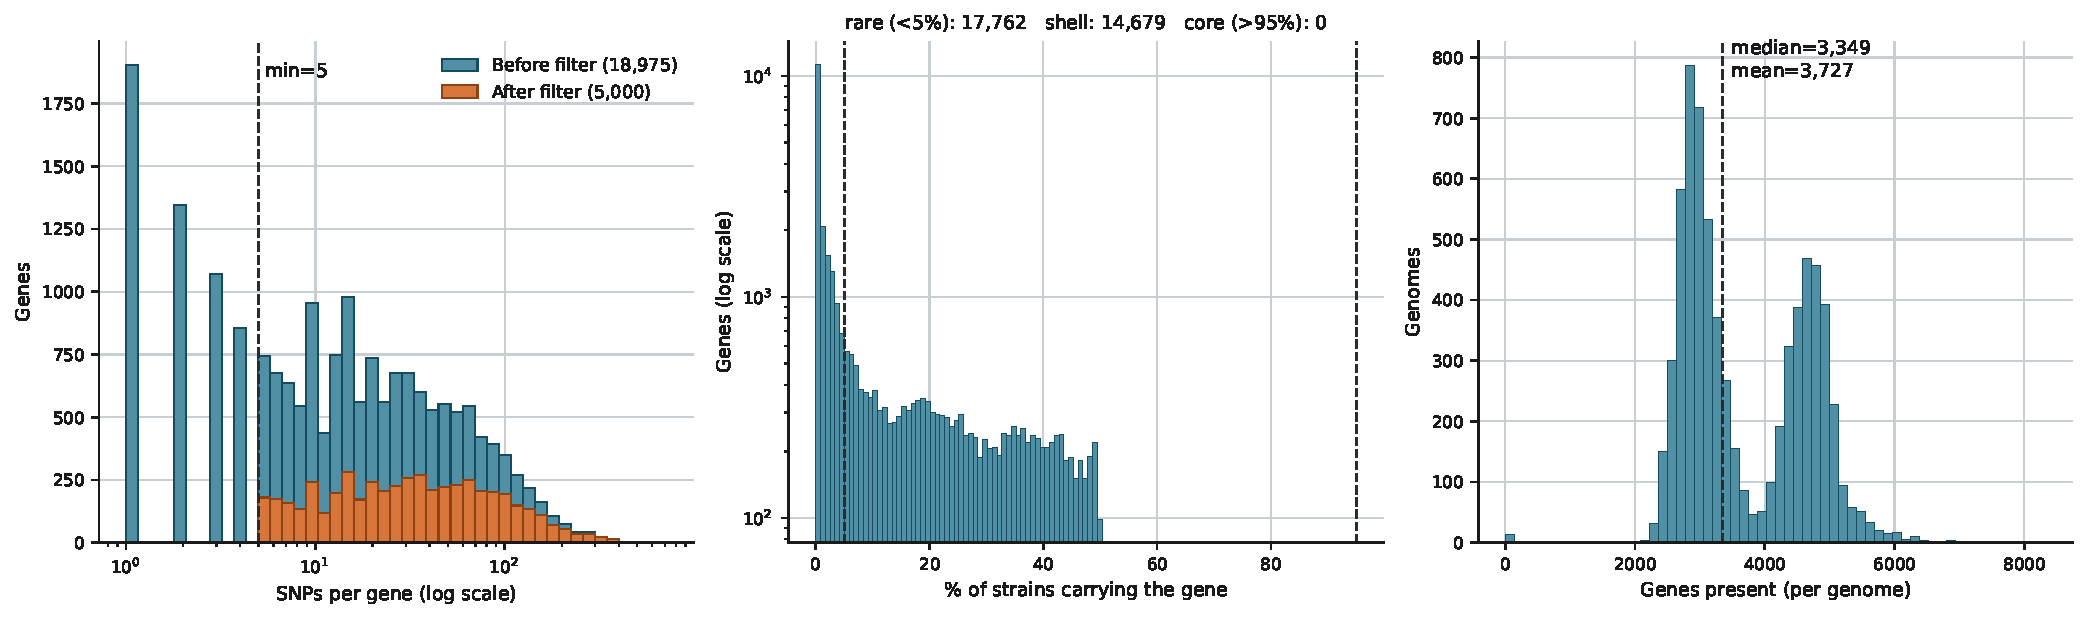
\includegraphics[width=\textwidth]{fig_gene_feature_space.pdf}
\caption{The gene feature space before and after filtering.}
\label{fig:gene_feature_space}
\fignote{\textbf{Left:} SNPs per gene across the 18{,}975 genes of the SNP view,
before and after the variability and importance filters cut them to 5{,}000.
\textbf{Centre and right:} the separate 32{,}441-gene presence and absence
catalogue, which is mostly rare genes: 17{,}762 are carried by under 5\% of strains
and none by more than 95\%, and a typical genome holds a median of 3{,}349 of them
against a mean of 3{,}727.}
\end{figure}

After filtering, 5,000 genes remain. These genes contain 262,225 SNPs. This corresponds to
approximately 49.0\% of the original variants. These genes differ widely in size: the smallest carries 5 SNPs, the median
32, the mean 52, and the largest 717. That distribution fed one last decision. Our first view
reads each gene as a fixed length block, which we set to 64 positions. Approximately 28\% of
the selected genes are longer than 64 SNPs and are truncated, the remaining genes are padded
with zeros and masked with zeros, so the padding does not contribute. A gene block has an
average of 35 positions out of 64 that are occupied by real positions. Most genes would waste
memory if the block were too long, while a shorter block would cause the median gene to be
cut.

\FloatBarrier
\subsection{Preprocessed Data and the Three Evaluation Splits}
\label{subsec:splits}

The splits determine what a score measures, because of which we give a detailed account of
how we split the data. Approximately 15 percent of each split is for testing, another 15
percent of each split is for validation, and approximately 70 percent is for training. The
test set is never used in the model selection or tuning; it is not touched until the final
evaluation, and every split has been performed with the same fixed random seed (42), which
means that any number reported in this research can be exactly re-generated by running the same
code. We constructed three splits and they address three questions.
Table~\ref{tab:splits} gives their sizes and
Figure~\ref{fig:split_composition} draws the same three partitions as bars, so
that the one split whose training and validation sizes are not round can be seen at
a glance.

\vspace{1em}

The random split assigns strains via shuffling, stratified on the ampicillin label to achieve
class balance across the three sets. This results in a training set of 4,872 strains, a
validation set of 1,045 and a test set of 1,045. It is the normal setting, and the one that is
used in the majority of published work; the related strains can fall on both sides, and do.
The partition sizes remain the same but the partition balancing takes into account the
eight-way phylogroup assignment, each lineage group being represented in each of the three
sets in the same proportion as it would be in the collection as a whole. This does not control
class balance.

We just want to clarify what this second split is, as it can be very easily inflated. It is a
stratified split, as opposed to a holdout. By design, every phylogroup appears on both sides so
it is not testing how the model performs on a lineage it has never seen before. What it tests
is the extent to which the result is influenced by the choice of stratification variable. This
is a weaker question than the one we wished to answer, and Section~\ref{sec:discussion} tells
what happened when we first treated it as one that answered the stronger question.

The train/test split answering that more stringent question is the sequence-type lineage
holdout, and is the one upon which the central result of this research is built, so we will
describe its construction in full. Strains each have a multi-locus sequence type, a generic
label in bacterial genomics that clusters strains based on shared descent in the recent past
and is much more specific than phylogroup. We extracted it from the metadata provided on
strains, and rather than assigning sequence type by the position or row in the genome table, we
mapped the metadata identifying number to recover a sequence type for the large majority of the
collection.

Two rules were set prior to examining any result. In the absence of a sequence type, any
strain was assigned to training as an unlabelled group cannot be held out safely. If the
number of sequences in a collection type was more than five percent, then it was also put in
training. The other rule is equally important. Type 73 represents approximately an eighth of the entire
dataset. If that clone has a relatively large number of different strains found in the test
set, the test will mostly be measuring this particular clone. This does not measure how well
the model will work on novel lineages. The rest of the sequence types were then allocated
whole to training, validation or test by a seeded permutation walk which successively adds
groups until the desired proportion of genomes in each partition is reached.
Figure~\ref{fig:st_distribution} shows the size distribution these rules had to work around.

\begin{figure}[htb]
\centering
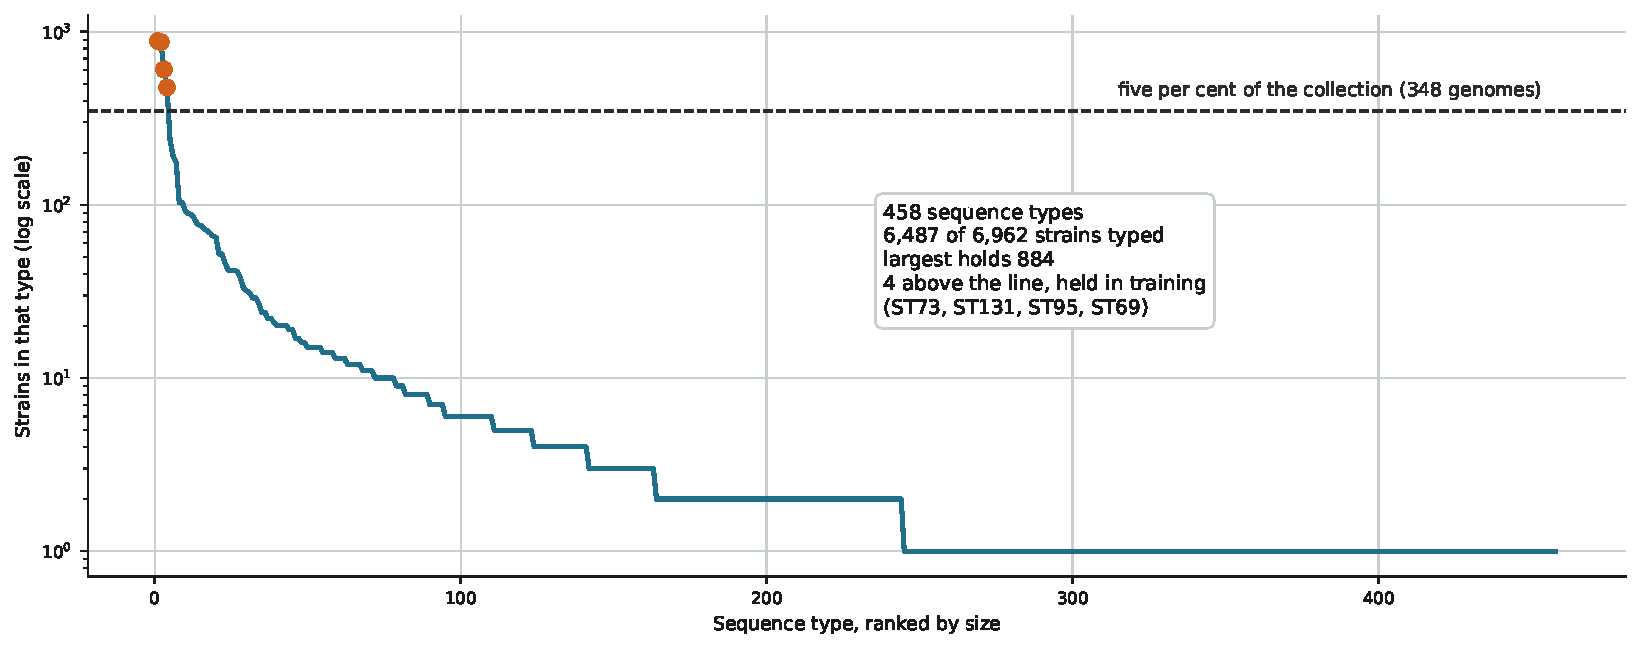
\includegraphics[width=\textwidth]{fig_st_distribution.pdf}
\caption{The 458 sequence types, ranked by size.}
\label{fig:st_distribution}
\fignote{A few types are very large and most are very small. The largest holds 884
strains, nearly one genome in eight, and four types sit above five per cent of the
collection. Those four, ST73, ST131, ST95 and ST69, are placed in training, so that
no test set can be dominated by a single clone.}
\end{figure}

We kept whole groups in the same partition. Owing to this, there are no ideal percentages of
the split. A chance division would appear less lopsided. This effect is reflected in our data
split as well. The holdout uses a training set of 4,836 strains, a
validation set of 1,081 and a test set of 1,045. No sequence type was observed to be present in
more than one partition (as opposed to assuming this), and Section~\ref{subsec:prevmatch}
describes an almost identical scan of the resulting test set, with no duplicate sequence types
found. The same point of method is used for all 3 splits. This 5,000 gene selection mentioned
earlier in this section under Data Reduction is re-fitted on each split's training partition
instead of being computed only once and used for each split. The definition of the pipeline
used an earlier version that leaked information between splits, which was fixed prior to any
results in this research. Refitting per split indicates that each split generates its ranking of
informative genes. It comes as a surprise to note that the holdout's gene set overlaps the
random split's by less than half, indicating that the resistance signal is not located in a
few genes but in many genes that are partly interchangeable.

\begin{table}[htb]
\centering
\caption{The three evaluation splits and the partition sizes they produce. Only the
third assigns whole groups, which is why its training and validation sizes are not
round.}
\label{tab:splits}
\small
\begin{tabular}{|l|l|r|r|r|}
\hline
\textbf{Split} & \textbf{Balanced on} & \textbf{Train} & \textbf{Val} & \textbf{Test} \\
\hline
Random & Ampicillin label & 4{,}872 & 1{,}045 & 1{,}045 \\ \hline
Phylogroup-stratified & Eight-way phylogroup & 4{,}872 & 1{,}045 & 1{,}045 \\ \hline
Sequence-type holdout & Whole sequence types, none shared & 4{,}836 & 1{,}081 & 1{,}045 \\ \hline
\end{tabular}
\vspace{0.4em}

\noindent\footnotesize\textit{Note:} Every row sums to 6{,}962. Only the sequence-type holdout
assigns whole groups at a time, which is why its training and validation partitions are not
round numbers; its test partition happens to land on the same 1{,}045 as the other two.
\end{table}

\begin{figure}[htb]
\centering
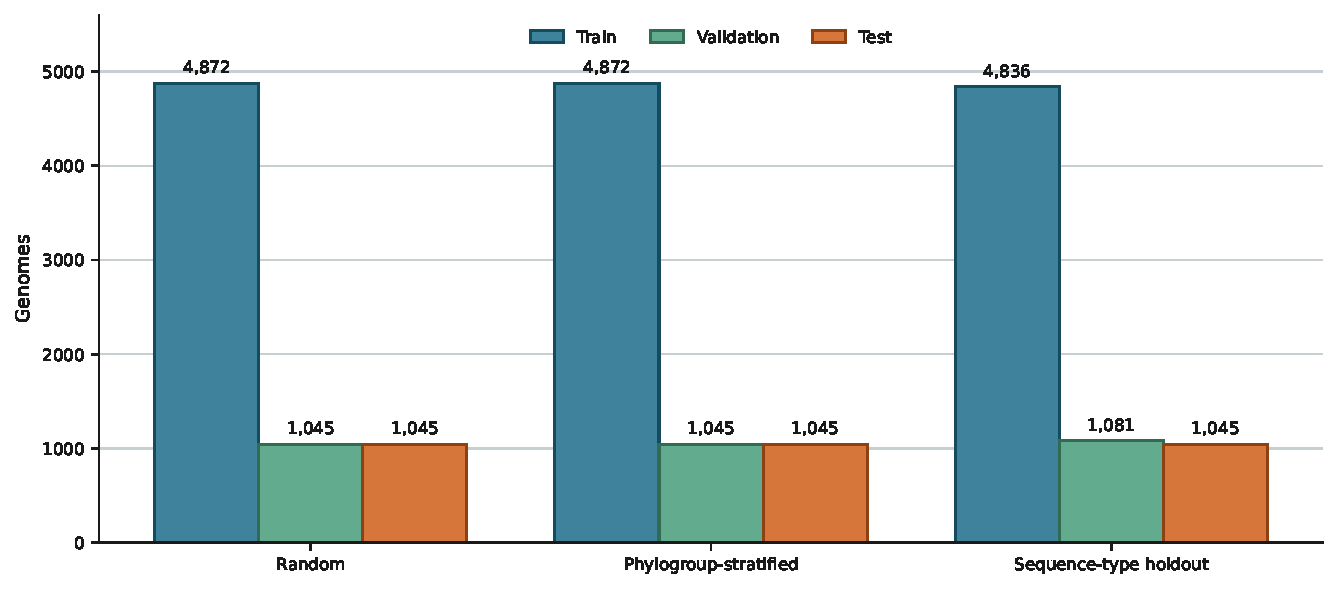
\includegraphics[width=\textwidth]{fig_split_composition.pdf}
\caption{Train, validation and test sizes for the three splits of
Table~\ref{tab:splits}.}
\label{fig:split_composition}
\fignote{The same 6{,}962 genomes are partitioned three different ways. Only the
sequence-type holdout keeps whole groups together, which is why its training and
validation partitions are not round.}
\end{figure}

For each split we also record the number of labelled strains and the resistance prevalence in
each partition, per antibiotic. The lower bound of precision recall AUC will be determined by
prevalence, meaning that a lower prevalence will result in a lower score even if the model is
equally good. The effects are greatest for the holdout, as forcing the largest clones into
training causes a shift in prevalence downwards for all of the antibiotics. Reporting the
prevalence with the score enables a reader to distinguish a drop because of a tougher test set
from a drop because of a lower floor. Figure~\ref{fig:split_prevalence_shift} shows how
large that shift is for each split.

\begin{figure}[htb]
\centering
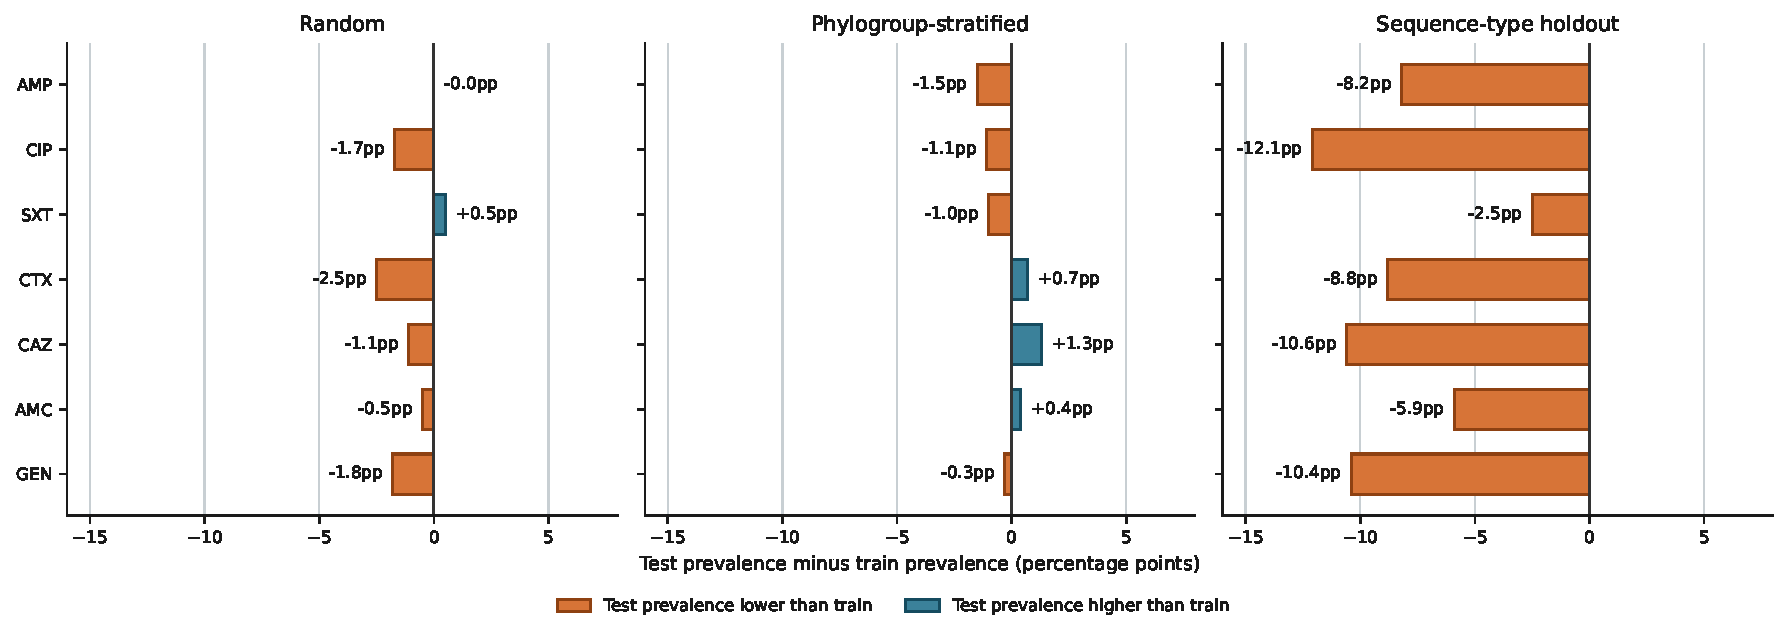
\includegraphics[width=\textwidth]{fig_split_prevalence_shift.pdf}
\caption{Test-minus-train resistance prevalence, in percentage points, per
antibiotic and per split.}
\label{fig:split_prevalence_shift}
\fignote{The random and phylogroup-stratified splits stay within 2.5 points and move
in both directions. The sequence-type holdout moves downwards for every antibiotic,
by 2.5 to 12.1 points, and since the no-skill floor of precision recall AUC is the
prevalence itself, part of the drop reported in Chapter~\ref{ch:results} follows from
this shift rather than from the model.}
\end{figure}

Now combining the three genomic views with the encoding of the phylogroup, the labels and
their mask provides the six arrays that are actually passed to the model, which are contained
in Table~\ref{tab:views}.

\begin{table}[htb]
\centering
\caption{Arrays produced by the preprocessing pipeline: four feature
representations, followed by the label matrix and its mask.}
\label{tab:views}
\small
\begin{tabular}{|l|l|l|l|}
\hline
\textbf{Representation} & \textbf{Shape} & \textbf{Type} & \textbf{What it captures} \\
\hline
SNP blocks by gene    & $6{,}962 \times 5{,}000 \times 64$ & int8    & mutation patterns inside genes \\ \hline
Gene presence/absence & $6{,}962 \times 32{,}441$          & uint8   & genes acquired from elsewhere \\ \hline
Per-gene statistics   & $6{,}962 \times 5{,}000 \times 4$  & float32 & coarse gene-level variation \\ \hline
Phylogroup one-hot    & $6{,}962 \times 8$                 & float32 & broad lineage \\ \hline
Labels                & $6{,}962 \times 7$                 & bool    & resistant or susceptible \\ \hline
Label mask            & $6{,}962 \times 7$                 & bool    & which labels were measured \\ \hline
\end{tabular}
\vspace{0.4em}

\noindent\footnotesize\textit{Note:} These six arrays are everything the model receives. The
mask is what allows an untested strain and drug combination to be skipped rather than imputed.
\end{table}

Two characteristics of this data set set the stage for everything that follows. It is broad
and short: there are still far more features than strains even after dimensionality reduction,
so the design favors gradient boosting over a large network. And it is patchy: antibiotic
coverage ranges from 49 to 87 per cent according to drug while prevalence ranges from 12 to 50
per cent, meaning no averaged score across the seven antibiotics serves it well; hence each
result in Chapter~\ref{ch:results} is reported per drug, as well as on average.

\vspace{1em}

A single collection does not provide an answer to the question of whether or not an approach
travels. We use a second, independent set of \textit{E. coli} genomes that were collected at
the University of Giessen and published by Ren et al.~\cite{Ren2022}. Isolates were from human
and animal clinical specimens and susceptibility was done by automated testing and interpreted
according to EUCAST breakpoints. Ren et al.\ report 987 Giessen isolates in total
(Table~\ref{tab:summary}); the subset we use is the 809 that carry a complete
result for all four of the antibiotics shared with our panel, which is the same
809 used by Siddiqui and Tarannum~\cite{siddiqui2025amrensemble}. Those 809
strains are described by 60,936 SNP positions each. Its composition is shown in
Table~\ref{tab:giessen}.

\begin{table}[htb]
\centering
\caption{Composition of the external Giessen dataset.}
\label{tab:giessen}
\small
\begin{tabular}{|l|r|r|r|}
\hline
\textbf{Antibiotic} & \textbf{Resistant} & \textbf{Susceptible} & \textbf{Prevalence} \\
\hline
CIP & 366 & 443 & 0.452 \\ \hline
CTX & 358 & 451 & 0.443 \\ \hline
CAZ & 276 & 533 & 0.341 \\ \hline
GEN & 188 & 621 & 0.232 \\ \hline
\end{tabular}
\vspace{0.4em}

\noindent\footnotesize\textit{Note:} Every isolate carries a result for all four drugs, so no
mask is needed here. Prevalence is roughly two to three times the Arcadia value for the same
drug, which is why the retention figures in Chapter~\ref{ch:results} cannot be read as
like-for-like.
\end{table}

There are two disparities with the Arcadia data that influence its use. The first one is the
reference. In Giessen variants are listed in order of a single reference genome (columns are
ordered along the chromosome) while Arcadia uses a pan-genome (the ordering of the columns has
no meaning). This difference is not an inconvenience: it makes the locality test in
Section~\ref{subsec:cnnfail} possible because we have one set of data for which locality
should matter, and one set for which it should not. The second is the two feature spaces have
no overlap. The model trained on Arcadia cannot be used at Giessen, since there is no shared
feature vector, so anything we do across the two collections must be a comparison of methods,
as Section~\ref{sec:comparisons} states.

\vspace{1em}

Also, there is a difference in the label names. The Giessen phenotypes are interpreted against
the EUCAST breakpoints, and the Arcadia phenotypes are interpreted according to a different
standard. Breakpoint differences between the two also exist for the same drug, and this could
contribute to performance differences between collections, and not only to the model. We are
unable to separate the two effects with the data available and designate it as a limitation
for any cross-collection comparison. This dataset consists of 809 strains with results for all
four types of drugs, unlike Arcadia where some of the labels are missing, so masking is not
necessary. The numbers were randomly split by ciprofloxacin into 647 for training, 81 for
validation and 81 for testing. The test partition is small and that is why the Giessen
confidence intervals in Chapter~\ref{ch:results} are wider than those for Arcadia.

\FloatBarrier
\section{Implementation of Selected Design}
\label{subsec:common_framework}

All of the settings below are global across the model. Most follow traditional practice and
are therefore included for completeness; a few are less obvious and are explained, where
necessary.

\subsection{Binary Classification Setup}

In the case of each antibiotic, the model aims to predict either resistance (labelled 1) or
susceptibility (labelled 0). The inputs are the three genomic views discussed in the top-level
overview and each raw score is transformed into a probability using the logistic sigmoid from
Equation~\eqref{eq:sigmoid}. All seven antibiotics are predicted in the same forward pass,
making it a multi-label problem instead of a multi-class problem: a strain may be resistant to
multiple drugs simultaneously and the predictions do not have to compete with each other.

\subsection{Handling Class Imbalance}

Susceptible strains by far outnumber resistant ones for various drugs, which poses a very real
trap: a model predicting susceptible in all cases scores highly on accuracy and is useless,
but which is approximated well by a model that predicts the majority class as the easiest way
to minimize the loss.

To avoid this, the resistant and susceptible samples are reweighted in inverse proportion to
their frequency of occurrence, such that a mistake in getting a rare resistant strain is much
costlier. In the classical tree-based learners it can be accomplished by the
\texttt{scale\_pos\_weight} parameter,
\begin{equation}
\text{\texttt{scale\_pos\_weight}} = \frac{N_{\text{neg}}}{N_{\text{pos}}},
\label{eq:scale_pos_weight}
\end{equation}
where $N_{\text{neg}}$ and $N_{\text{pos}}$ are the numbers of susceptible and resistant
samples. In Logistic Regression and Random Forest, this is accomplished by using balanced
class weights, and in the neural lenses, by using positive class weighting in the loss. For
this reason, we use precision-recall AUC and not accuracy during the evaluation as accuracy
would conceal precisely the failure we want to avoid.

\subsection{Data Splitting Strategy}

The model is trained and tested in three settings which are generated in
Section~\ref{subsec:splits}: random split, phylogroup-stratified split, and sequence-type
lineage holdout. The reporting of all three, and the space between them, is part of the
evaluation design. A validation set is employed for tuning; a final test set is only employed
for the final evaluation and a fixed random seed of 42 is used throughout.

\subsection{Threshold Selection}
\label{subsec:threshold_selection}

To arrive at the final decision, we use a constant probability threshold of 0.5 for each of the
antibiotics, as in Equation~\eqref{eq:decision}. This is the indifferent option. It places the same emphasis on the two kinds of errors. But in
clinical practice this is not the case. The issue of predicting a resistant strain as being
susceptible can result in administering a drug that is not effective. The reverse error is
only going to result in picking another drug.
A recall-oriented adjustment was made according to the $F_{\beta}$ score,
\begin{equation}
F_{\beta} = \frac{(1 + \beta^2)\cdot\text{Precision}\times\text{Recall}}{\beta^2\cdot\text{Precision} + \text{Recall}},
\label{eq:fbeta}
\end{equation}
with $\beta = 2$ to give four times as much weight to recall as to precision, would lower the
threshold and capture more resistant strains while increasing the number of false alarms. To
avoid tuning the numbers in our favour, all headline results in this research have been reported
at the neutral threshold of 0.5 and then per-antibiotic threshold tuning has been directly
tested in Section~\ref{sec:perfeval}, fitting the threshold on validation and applying it to
test.

\FloatBarrier
\subsection{Optimization and Training Schedule}

The training of the neural lenses, the gate and the fusion step is done in a simultaneous way,
so that each lens learns to be useful in conjunction with the others and not optimised alone.
The objective consists of three terms: a binary cross-entropy loss over the fused scores, the
entropy regulariser in Equation~\eqref{eq:entropy_reg}, and an auxiliary loss on each lens. This extra loss term is important. In its absence, a lens which is momentarily disregarded by
the gate achieves extremely limited gradient. This leads to its cessation of improvement. This
problem is avoided by the auxiliary loss. It aids all lenses in continuing to learn, even when
they are not being selected by the gate. Optimization
employs the AdamW optimiser that keeps the weight decay and gradient update decoupled, and the
learning rate of $10^{-3}$, annealed on a cosine schedule over the epoch budget, weight decay
of $10^{-4}$, batch size of 16, gradient clipping of norm 1.0, and mixed-precision training,
with up to 50 epochs and early stopping after 8 consecutive no-improvement epochs of
validation mean precision-recall AUC. The inclusion of gradient clipping is because, when
attention is placed over 32{,}441 genes, the gradients can sometimes be quite large, causing
the training to become unstable. The five classical base learners are trained individually via
5-fold cross validation, with out-of-fold predictions, which are then used to fit the
logistic-regression meta-learner, along with the neural probabilities. The most important
hyperparameters are summarised in Table~\ref{tab:hyperparameters}.

{\small\setlength{\tabcolsep}{5pt}
\begin{longtable}{|>{\raggedright\arraybackslash}p{2.9cm}|>{\raggedright\arraybackslash}p{10.7cm}|}
\caption{Hyperparameter configuration for the classical base learners and the neural model.}
\label{tab:hyperparameters}\\
\hline
\textbf{Component} & \textbf{Key Hyperparameters} \\
\hline
\endfirsthead
\hline
\textbf{Component} & \textbf{Key Hyperparameters} \\
\hline
\endhead
\hline
\multicolumn{2}{r}{\footnotesize\textit{Continued on the next page}}\\
\endfoot
\hline
\endlastfoot
XGBoost (gene) &
n\_estimators=1500; max\_depth=5; min\_child\_weight=5; learning\_rate=0.05;
subsample=0.8; colsample\_bytree=0.7; reg\_alpha=0.1; reg\_lambda=1.0; gamma=0.1;
tree\_method='hist'; scale\_pos\_weight=$N_-/N_+$ per drug; early\_stopping\_rounds=150 \\ \hline
XGBoost (raw) &
chi\textsuperscript{2}-prefilter (top 50{,}000 SNPs); n\_estimators=1500; max\_depth=5;
learning\_rate=0.05; subsample=0.8; colsample\_bytree=1.0; colsample\_bynode=0.5;
reg\_alpha=0.1; reg\_lambda=1.0; tree\_method='hist'; scale\_pos\_weight=$N_-/N_+$ per drug;
early\_stopping\_rounds=150 \\ \hline
LightGBM &
n\_estimators=1500; num\_leaves=63; max\_depth=6; min\_child\_samples=20; learning\_rate=0.05;
subsample=0.8; subsample\_freq=1; colsample\_bytree=0.7; reg\_alpha=0.1;
reg\_lambda=1.0; scale\_pos\_weight=$N_-/N_+$ per drug; early\_stopping\_rounds=150 \\ \hline
Random Forest &
n\_estimators=200; max\_depth=12; min\_samples\_leaf=10 \\ \hline
Logistic Regression (base) &
scikit-learn defaults (L2 penalty) \\ \hline
Neural lenses + MoE gate &
optimizer=AdamW; learning\_rate=$10^{-3}$ with cosine annealing;
weight\_decay=$10^{-4}$; batch\_size=16;
epochs=50; patience=8; grad\_clip=1.0; mixed precision; entropy weight=0.01; seed=42 \\ \hline
Stacking meta-learner &
Logistic Regression (L2, $C=1.0$), per antibiotic; 5-fold out-of-fold inputs \\ \hline
\end{longtable}}



\chapter{Result Analysis}
\label{ch:results}

This chapter outlines what our models produced and what those numbers mean. First
we describe the measures that we used in evaluating performance and the results
of the proposed model, and then decompose the model, layer upon layer, to see
where its performance actually comes from. The remainder of the chapter
turns to the evidence that matters most for this research's central claim: how
the model behaves under a genuine lineage holdout, on a separate collection,
and when the genes it claims to rely on are put to the test.

\section{Performance Evaluation}
\label{sec:perfeval}

The smaller group are the resistant strains, and
even for a single antibiotic only about one in five strains is resistant, so plain
accuracy would not reveal the problem: a model that declared every strain susceptible
would still seem accurate, but would be useless in a clinic. The primary
metric that we are interested in is the area under the precision--recall curve
(PR-AUC), which captures the performance of a model in terms of
precision-recall at all threshold levels and does not encourage a model to
make majority class predictions. It is defined as

\begin{equation}
\text{PR-AUC} = \sum_{n} \left( R_n - R_{n-1} \right) P_n
\end{equation}

where $P_n$ and $R_n$ are the precision and recall at the $n$-th threshold.

We also report a few other measures, since there is no single number which
tells the entire story. Matthews Correlation Coefficient (MCC) employs all
four cells of the confusion matrix simultaneously, and remains truthful in
case of imbalanced classes:

\begin{equation}
\text{MCC} = \frac{TP \times TN - FP \times FN}
{\sqrt{(TP+FP)(TP+FN)(TN+FP)(TN+FN)}}
\end{equation}

MCC can be between $-1$ and $+1$ (where $0$ indicates model guessing), and all
values are calculated per antibiotic using a one-versus-rest approach. F1 is
the harmonic mean of precision and recall; F2 weighted recall four times
higher, since failing to identify a drug-resistant strain is worse than
falsely labelling a susceptible strain resistant (it sends a patient to a drug that will not
work, whereas a false positive just wastes a treatment slot):

\begin{equation}
F_1 = 2 \cdot \frac{P \cdot R}{P + R},
\qquad
F_2 = 5 \cdot \frac{P \cdot R}{4P + R}
\end{equation}

We show accuracy for thoroughness, but we do not use it. Measures of machine
learning are inadequate by themselves to tell a clinician whether a tool is
safe, and so we also report the microbiology vocabulary. A \emph{very major
error} (VME) is a resistant strain called susceptible, which is the
dangerous case; a \emph{major error} (ME) is the reverse, which costs a drug
option but does not put the patient directly at risk; and \emph{categorical
agreement} (CA) is the proportion of strains on which our call matched
the laboratory result. All these evaluations determine three
things: the degree to which the model ranks strains well (PR-AUC), the degree
to which it makes balanced decisions at some threshold (MCC, F1, F2), and
whether its errors would be tolerated in a hospital (VME, ME, CA).

\vspace{1em}

All results in this section use the curated dataset and the random split of
Section~\ref{sec:data}. All measures of all seven antibiotics have been
reported in Table~\ref{tab:main}, and plotted in Figure~\ref{fig:pr_curves} as
a background to the PR-AUC column. That figure also carries the lineage-holdout
curves in red, which belong to Section~\ref{subsec:prevmatch} and should be
ignored for now; they are drawn alongside so that the reader can return to a
single figure once both splits have been introduced. For this section, only the
blue curves are relevant.

\begin{table}[htb]
\centering
\caption{TriLens-MoE-Stack on the random split, per antibiotic.}
\label{tab:main}
\small
\begin{tabular}{|l|r|r|r|r|r|}
\hline
\textbf{Antibiotic} & \textbf{PR-AUC} & \textbf{MCC} & \textbf{F1} & \textbf{F2} & \textbf{Accuracy} \\ \hline
CIP & \textbf{0.9773} & 0.9088 & 0.9282 & 0.9197 & 0.9692 \\ \hline
AMP & 0.9440 & 0.7866 & 0.8932 & 0.8917 & 0.8933 \\ \hline
CTX & 0.9019 & 0.7904 & 0.8173 & 0.8126 & 0.9530 \\ \hline
SXT & 0.8352 & 0.6954 & 0.7875 & 0.7730 & 0.8707 \\ \hline
CAZ & 0.8299 & 0.6928 & 0.7290 & 0.7169 & 0.9356 \\ \hline
AMC & 0.7482 & 0.5237 & 0.6563 & 0.6250 & 0.8035 \\ \hline
GEN & \textbf{0.7037} & 0.6095 & 0.6386 & 0.5915 & 0.9341 \\ \hline
\textbf{Average} & \textbf{0.8486} & \textbf{0.7153} & \textbf{0.7786} & \textbf{0.7615} & \textbf{0.9085} \\ \hline
\end{tabular}
\vspace{0.4em}

\noindent\footnotesize\textit{Note:} Ciprofloxacin has the highest PR-AUC (0.9773) and
gentamicin the lowest (0.7037), the spread the text below discusses; the last row averages
across all seven antibiotics. Bold marks the extreme values of the PR-AUC column, best and
worst alike, and the average row.
\end{table}

\FloatBarrier
\begin{figure}[htb]
\centering
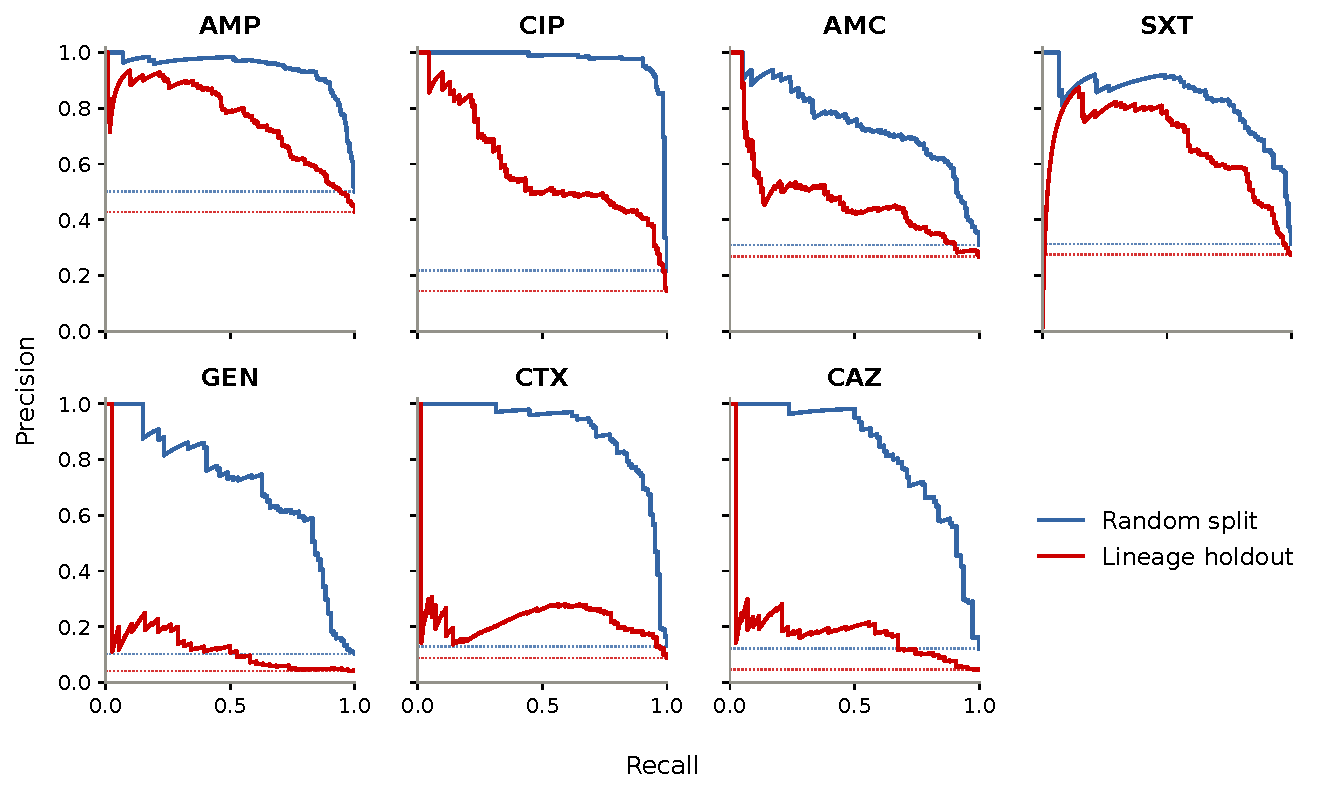
\includegraphics[width=\textwidth]{fig_pr_curves.pdf}
\caption{Precision--recall curves for all seven antibiotics.}
\label{fig:pr_curves}
\fignote{Blue is the random-split test set discussed in this section; red is the
sequence-type lineage holdout, which is not analysed until
Section~\ref{subsec:prevmatch} and is drawn here only so the two can be compared on
one set of axes. The dotted lines are the no-skill baselines, one per split.}
\end{figure}

The average PR-AUC is 0.849, yet the average conceals a broad distribution, and
the interesting part is the spread. The clearest case is ciprofloxacin, at 0.9773 with MCC
0.9088, which is close to a practical ceiling for this kind of data, followed
by ampicillin at 0.9440. On the other hand, gentamicin comes in at 0.7037
and amoxicillin-clavulanate at 0.7482, meaning the spread of best to worst is
nearly 0.27 for models trained on exactly the same genomes with the exact same
architecture.

The accuracy column is different from the others. Gentamicin has the lowest
PR-AUC value, but high accuracy value of 0.9341 as the proportion of strains
resistant to gentamicin is small, so a model can achieve a high accuracy, but
fail to detect many resistant strains. This is the same trap as above, and
the reason accuracy is not our primary measure. As far as a hospital is concerned, it
is the type of error that the model produces, of which the results are
documented in Table~\ref{tab:clinical}.

\FloatBarrier
\begin{table}[htb]
\centering
\caption{Clinical error rates at a threshold of 0.5, ordered by very major error
rate.}
\label{tab:clinical}
\small
\begin{tabular}{|l|r|r|r|l|}
\hline
\textbf{Antibiotic} & \textbf{VME} & \textbf{ME} & \textbf{CA} & \textbf{Meets CLSI limits} \\ \hline
CIP & \textbf{0.086} & 0.015 & 0.969 & No (ME only) \\ \hline
AMP & 0.109 & 0.104 & 0.893 & No \\ \hline
CTX & 0.190 & 0.026 & 0.953 & No (ME only) \\ \hline
SXT & 0.236 & 0.080 & 0.871 & No \\ \hline
CAZ & 0.291 & 0.033 & 0.936 & No \\ \hline
AMC & 0.394 & 0.108 & 0.804 & No \\ \hline
GEN & \textbf{0.436} & 0.023 & 0.934 & No (ME only) \\ \hline
\end{tabular}
\vspace{0.4em}

\noindent\footnotesize\textit{Note:} Ciprofloxacin has the lowest very major error (VME) rate at
0.086 and gentamicin the highest at 0.436. No antibiotic meets both CLSI limits at once;
``No (ME only)'' means only the major-error limit is met.
\end{table}

Ciprofloxacin reappears as the strongest, having a VME of 0.086, and a
categorical agreement of 0.969. Gentamicin is weakest with 0.436 (almost half
of all resistant strains would be reported sensitive) and
amoxicillin-clavulanate is almost as poor (0.394). The ordering is important,
as an almost identical ordering is rediscovered under the lineage holdout in
Section~\ref{subsec:prevmatch} in an entirely different way.

\vspace{1em}

The categorical agreement column is the same as the accuracy column of
Table~\ref{tab:main}, and this is not by chance. During data preparation
the intermediate results were grouped with the resistant results, so the
intermediate category no longer exists in this dataset. Categorical
agreement therefore reduces to binary accuracy here.
Gentamicin illustrates this point clearly, with a categorical agreement of 0.934 versus
a VME of 0.436. On the same strains, the same model is seen to be strong by
one measure and unusable by the other.

\vspace{1em}

The CLSI limits require both the VME and ME rates to stay under three
percent. Three antibiotics satisfy the major error limit, which are
ciprofloxacin at 0.015, gentamicin at 0.023 and cefotaxime at 0.026 but none
satisfy the very major error limit, therefore, the model is not yet prepared
to be used as a diagnostic test.

\vspace{1em}

The obvious response is that the fixed 0.5 threshold was never tuned to
clinical cost, and that the numbers above could be an artefact of positioning
the cut. To do this, we trained a threshold for each antibiotic on the
validation set, constraining the $F_2$ objective of Equation~\eqref{eq:fbeta}
and capping the major error rate, and assessed each on the test set. While the
tuning for $F_2$ moves the mean very major error rate only from 0.249 to
0.210, still far above the limit of 0.03, and forcing the major error rate to
remain inside the limit pushes the mean very major error rate to 0.437,
neither rescues the model. In fact, none of the antibiotics was able to achieve both
thresholds at any threshold value that we tested, because shifting the cut
trades one kind of error against the other instead of
cutting down on both. It is not the position of the cut that drives the clinical
shortfall, however, but the model's ability to separate the two classes, a point
the heritability comparison in Section~\ref{subsec:published} also supports. As
such, future work should not focus on calibration, but on the feature
representation.

\FloatBarrier
\section{Analysis of Design Solutions}
\label{subsec:layerabl}

Each neural lens reads a different part of the genome and a gate determines
the trustworthiness of each lens, with five classical learners combined by a
stacking layer. To determine whether each part is warranted, we removed each
component in turn and measured the impact on performance. We trained three variants using the same data,
seed and test set.

\begin{itemize}
  \item \textbf{Stage 1.} The three lenses only. They average their outputs
  with equal weighting. No gate is used.
  \item \textbf{Stage 2.} The three lenses and the mixture-of-experts gate,
  such that the model learns the extent to which to rely on individual lenses
  on individual samples and antibiotics. This is the neural part of the model
  on its own.
  \item \textbf{Stage 3.} The complete model in which the neural output is
  appended with the five classical base learners via the meta-learner.
\end{itemize}

Table~\ref{tab:ablation} sets the three variants side by side, per antibiotic, with the gain
each stage adds over the one before it. Reading down a column shows how much of a drug's final
score was already in place before the classical learners were attached to it.

\begin{table}[htb]
\centering
\caption{Component ablation on the random split, with the PR-AUC gain each added
part contributes over the stage before it.}
\label{tab:ablation}
\small
\setlength{\tabcolsep}{3pt}
\resizebox{\textwidth}{!}{%
\begin{tabular}{|l|r|r|r|r|r|r|r|r|r|}
\hline
\textbf{Stage} & \textbf{AMP} & \textbf{CIP} & \textbf{AMC} & \textbf{SXT} & \textbf{GEN} & \textbf{CTX} & \textbf{CAZ} & \textbf{Avg} & \textbf{Gain} \\ \hline
Stage 1: lenses only    & 0.8920 & 0.9248 & 0.6249 & 0.7217 & 0.5168 & 0.8103 & 0.7267 & 0.7453 & N/A \\ \hline
Stage 2: + MoE gate     & 0.8970 & 0.9489 & 0.6347 & 0.7453 & 0.5835 & 0.8659 & 0.7893 & 0.7807 & +0.0353 \\ \hline
Stage 3: + stacking     & 0.9440 & 0.9773 & 0.7482 & 0.8352 & 0.7037 & 0.9019 & 0.8299 & \textbf{0.8486} & \textbf{+0.0679} \\ \hline
\end{tabular}
}
\vspace{0.4em}

\noindent\footnotesize\textit{Note:} The full model reaches an average PR-AUC of 0.8486;
classical stacking adds +0.0679 over stage 2, about twice the gate's own +0.0353 contribution.
\end{table}
\FloatBarrier

There are two points that are established. First, there is no dead weight: for
each and every antibiotic, the performance improves when it goes from Stage 1
to Stage 2 and then to Stage 3. Second, the parts do not aid equally.
Combining neural predictions with classical learners achieves on average
about 0.0679 more than the neural design alone, while the gate achieves only
0.0353. The neural lenses are useful, but not sufficient by themselves, and
thus the final model is best referred to as a hybrid rather than as a neural
model. Figure~\ref{fig:layer_ablation} breaks the same three stages down antibiotic by
antibiotic.

\begin{figure}[htb]
\centering
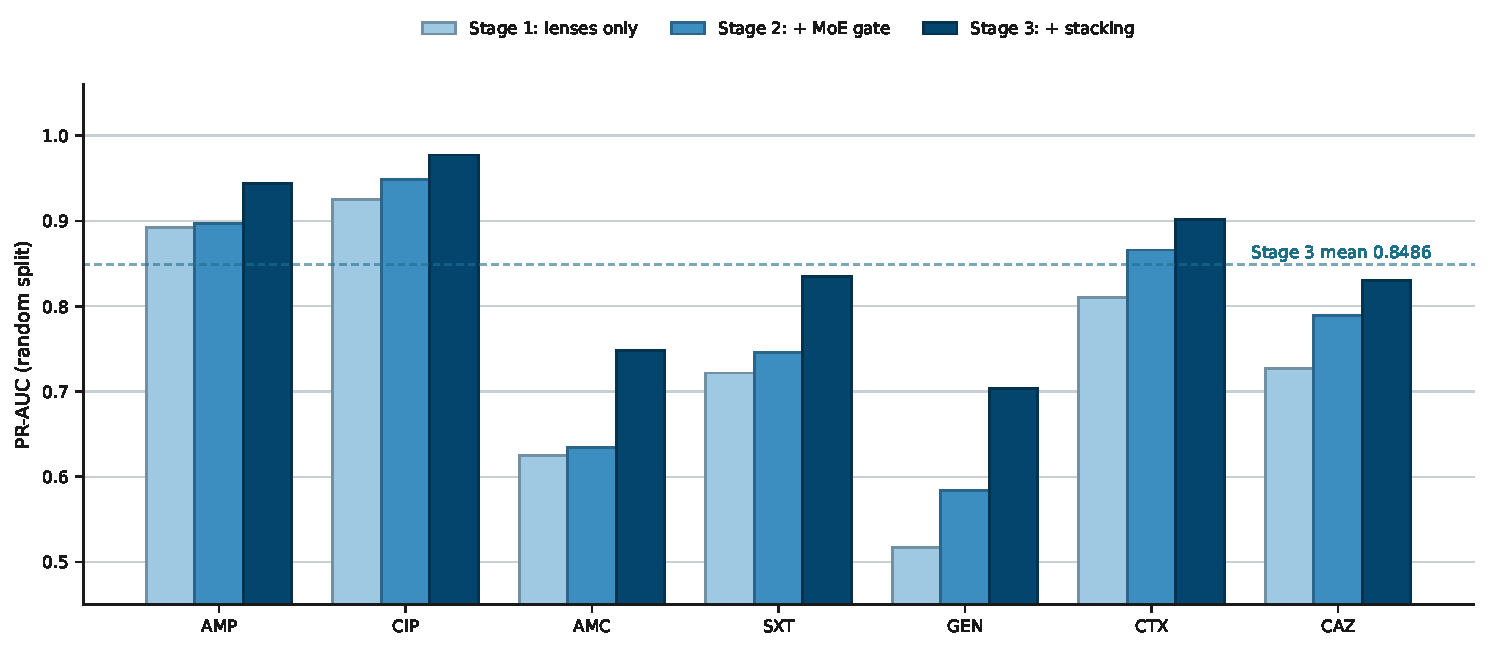
\includegraphics[width=\textwidth]{fig_layer_ablation.pdf}
\caption{The component ablation of Table~\ref{tab:ablation}, per antibiotic.}
\label{fig:layer_ablation}
\fignote{Every antibiotic improves from Stage 1 to Stage 2 and again from Stage 2 to
Stage 3, but the size of each step varies widely; gentamicin gains most from the
classical stacking layer.}
\end{figure}

The average weight assigned to each lens by the gate is shown in
Table~\ref{tab:gate}, and the weights by antibiotic in
Figure~\ref{fig:gate_routing}.

\begin{table}[htb]
\centering
\caption{Average gate weights on the test set. Each row sums to one.}
\label{tab:gate}
\small
\resizebox{\textwidth}{!}{%
\begin{tabular}{|l|r|r|r|}
\hline
\textbf{Antibiotic} & \textbf{Lens A (motif CNN)} & \textbf{Lens B (presence/absence)} & \textbf{Lens C (cross-antibiotic)} \\ \hline
AMP & 0.070 & 0.852 & 0.078 \\ \hline
CIP & \textbf{0.035} & 0.590 & 0.374 \\ \hline
AMC & 0.095 & 0.742 & 0.163 \\ \hline
SXT & 0.052 & \textbf{0.900} & 0.047 \\ \hline
GEN & 0.098 & 0.731 & 0.171 \\ \hline
CTX & 0.064 & 0.815 & 0.121 \\ \hline
CAZ & 0.044 & 0.835 & 0.122 \\ \hline
\end{tabular}
}
\vspace{0.4em}

\noindent\footnotesize\textit{Note:} Ciprofloxacin's Lens A weight of 0.035 is the lowest in the
table despite being the drug that lens was built for, and trimethoprim-sulfamethoxazole's Lens B
weight of 0.900 is the highest, closest to gate collapse; both are discussed below.
\end{table}

The trend is the same. Most of the weight of each antibiotic, 0.590 to 0.900,
is in Lens B, which reads which genes are present or absent, whereas Lens A,
the convolutional lens reading mutation patterns within genes, never goes
above 0.098. At least this is consistent with the biology as a large part of
the resistance in \textit{E. coli} is conferred by acquired genes.

\begin{figure}[htb]
\centering
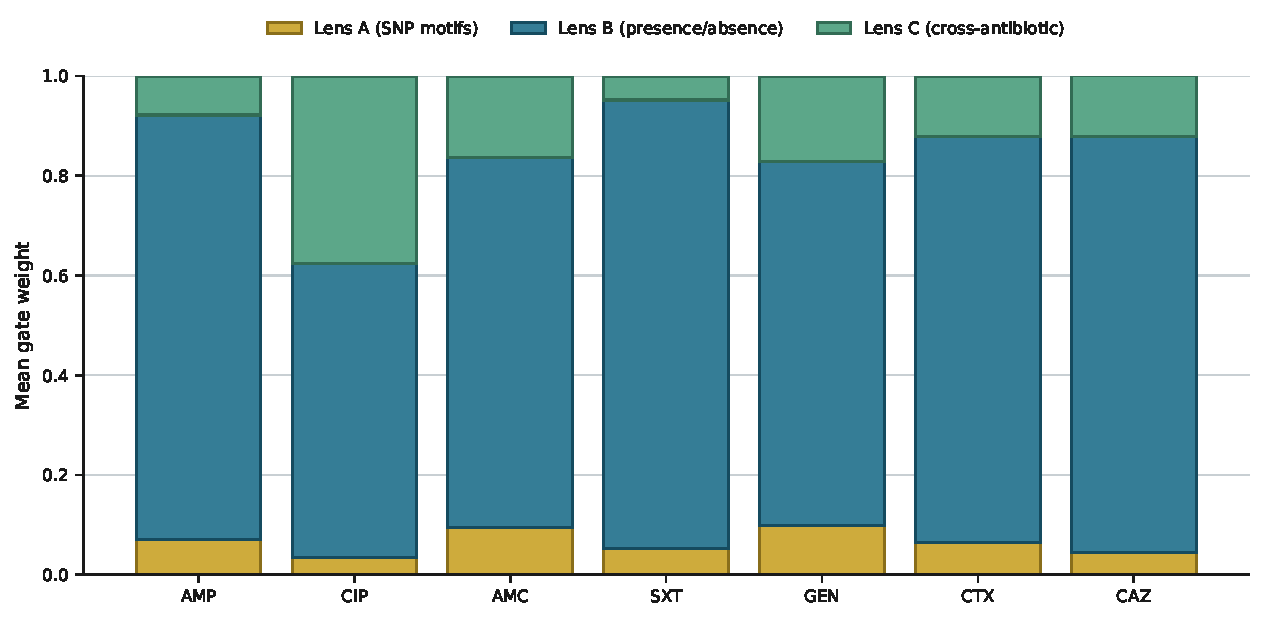
\includegraphics[width=\textwidth]{fig_gate_weights.pdf}
\caption{Mean gate weight assigned to each lens, by antibiotic, on the test set.}
\label{fig:gate_routing}
\fignote{The three weights sum to one for each antibiotic; these are the values of
Table~\ref{tab:gate} drawn as stacked bars.}
\end{figure}

\vspace{1em}

Ciprofloxacin is where the table stops agreeing with the design. The rationale
for the gate in Section~\ref{subsec:moegate} is a prediction: a drug whose
resistance is based on an acquired gene should route to Lens B, whereas a drug
whose resistance is based on a point mutation in a target enzyme should route
to Lens A. Ciprofloxacin is the most obvious point-mutation drug that we have
in our panel, and the one that our SHAP analysis suggests is related to
\textit{gyrA} and \textit{parC}; yet Lens A receives 0.035 for this drug, the
lowest value in the table. The prediction fails on the one antibiotic where it
was most testable. This is the highest value for Lens C, but it is difficult
to read from either direction. The lens shares drug-class head evidence, but
ciprofloxacin is the only fluoroquinolone in the panel and has no same-class
partner, and although its co-resistance refinement step may still link
ciprofloxacin to ceftazidime, which shares $\phi = 0.52$ in this collection
(Figure~\ref{fig:coresistance}), that is co-occurrence rather than
mechanism. On neither reading can 0.374 be taken as the gate finding the
mechanism.

\vspace{1em}

The gate hence informs us of the lens the model inclines on, which is
interesting to know, but its routing is not in the direction which the design
supposed. The same conclusion is drawn in the attention audit in
Section~\ref{subsec:attnfix}. A second reading of the table points the same
way. In the fold reported in Section~\ref{subsec:devadjust}, Lens B takes a
weight of 0.895. The other two lenses are pushed to virtually zero. This is
exactly the pattern the entropy penalty is meant to prevent. In the final
weights, trimethoprim-sulfamethoxazole reaches 0.900, even higher than that
fold. Three more drugs sit above 0.81: ampicillin at 0.852, ceftazidime at
0.835, and cefotaxime at 0.815. It seems
that the penalty would have slowed, but not stopped, collapse, and therefore,
these weights are possibly associated with optimisation-like dynamics as well
as with biology.

\FloatBarrier
\section{Final Design Adjustments}
\label{sec:designadj}

\FloatBarrier
\subsection{The Change of Dataset}
\label{subsec:ownprep}

An earlier phase of the project created its own set of features out of the
raw variant files. Filtering of variants was done by missingness and
frequency, followed by coding into binary columns and merging with the
phenotype table. This resulted in a 6{,}962 by 80{,}984 strain-by-feature
matrix. The screening of
various model families on it revealed two issues that were not related to the
models themselves: namely, our filtering criteria discarded variants based on
simple thresholds and no gene-level structure was present, which is precisely
what the proposed model reads. We thus relocated to the curated version
releases of Arcadia Science that had been previously quality checked and
mapped to genes, and all the experiments described in this research have used
that dataset.

The weakest of the families we tried was a one dimensional convolutional
network, and not merely because it needed tuning, but because a convolution
expects neighbouring columns to be related: those columns should have held
variants from nearby positions, whereas in the file the adjacent columns of
the matrix held variants from unrelated positions in the genome. The latter, one of our clearer
findings, is directly tested in Section~\ref{subsec:cnnfail} when we apply
that explanation to the curated data.

\FloatBarrier
\subsection{Adjustments Made During Development}
\label{subsec:devadjust}

Four further pieces of the final design came from problems encountered during
development rather than in planning. We had intended to have an entirely neural model. The ablation in
Section~\ref{subsec:layerabl} altered that: the neural lenses alone attained
0.7807 and including the classical learners boosted the model up to 0.8486,
thus, dropping them would have cost 0.068 to maintain the cleanliness of the
design. Second, the gate occasionally shifted to assigning a single lens
nearly the entire weight, such as 0.895 on Lens B in one of the
cross-validation folds and the other two almost on the lower end, when the
model is no longer a mixture of experts. To avoid this, we added a penalty term to the training loss based on the
entropy of the gate weights: it rises automatically as the weights become too
concentrated on a single lens, discouraging such a collapse. After this
penalty was applied, the weights recovered within two or three epochs.

\vspace{1em}

Third, Lens B computes attention over more than 32{,}000 genes with the absent
genes masked out, and in half precision this becomes invalid, because the
softmax breaks down over that many masked entries. Calculating just one softmax with single precision, with
the rest of the model in mixed precision, eliminated the problem with
virtually no performance penalty. Fourth, our first baseline reduced the SNP
matrix to 1024 principal components which was quick but lost the connection
between the SNP and the gene and we had a score of 0.803; all later models
were based on the gene-level view, which got us to 0.830.

\FloatBarrier
\section{Statistical Analysis}
\label{sec:statanalysis}

In our test set there are 1{,}045 strains and in some antibiotics there are
only a few hundred of known label, so one or two points difference can be
simply accidental. We resampled the test set (1{,}000 bootstrap resamples with
replacement) to recalculate PR-AUC, and used the 2.5th and 97.5th percentiles
as a 95\% confidence interval. The result is shown in Table~\ref{tab:ci} and
plotted in Figure~\ref{fig:ci_forest} as the intervals against the no-skill
baseline of the individual drugs, i.e., the range within which the raw scores
are most misleading: a PR-AUC has to be read against the prevalence of the
drug it represents, not against the other drugs in the column. The PR-AUC of
ampicillin, 0.944, sits above a no-skill baseline of roughly one resistant
strain in two. The score of gentamicin, 0.7037, appears smaller in absolute
terms, but its no-skill baseline is only about one resistant strain in ten.
Gentamicin's raw score is lower, yet it is the greater gain over chance.

\begin{table}[htb]
\centering
\caption{Bootstrap confidence intervals for the proposed model on the random-split
test set, from 1{,}000 resamples.}
\label{tab:ci}
\small
\begin{tabular}{|l|r|l|}
\hline
\textbf{Antibiotic} & \textbf{PR-AUC} & \textbf{95\% confidence interval} \\ \hline
AMP & 0.9440 & [0.919, 0.965] \\ \hline
CIP & 0.9773 & \textbf{[0.961, 0.990]} \\ \hline
AMC & 0.7482 & [0.680, 0.809] \\ \hline
SXT & 0.8352 & [0.773, 0.891] \\ \hline
GEN & 0.7037 & \textbf{[0.612, 0.786]} \\ \hline
CTX & 0.9019 & [0.851, 0.943] \\ \hline
CAZ & 0.8299 & [0.762, 0.882] \\ \hline
\textbf{Average} & \textbf{0.8486} & \\ \hline
\end{tabular}
\vspace{0.4em}

\noindent\footnotesize\textit{Note:} Ciprofloxacin's interval, [0.961, 0.990], is the tightest in
the table, backed by the most labelled data; gentamicin's, [0.612, 0.786], is the widest,
backed by the least. Bold marks the extreme values in a column, best and worst alike.
\end{table}

Gentamicin ranges 0.612 to 0.786, a range of nearly
0.18, and this is simply the result of few resistant strains, but
ciprofloxacin, which has more labelled strains and a stronger signal, has a
much smaller range. Any difference between two models on this test set must
therefore exceed this interval width before it can be termed significant.
None of the differences reported in this chapter between closely related
methods clears that bar. Figure~\ref{fig:ci_forest} plots the same intervals against
each antibiotic's no-skill baseline.

\begin{figure}[htb]
\centering
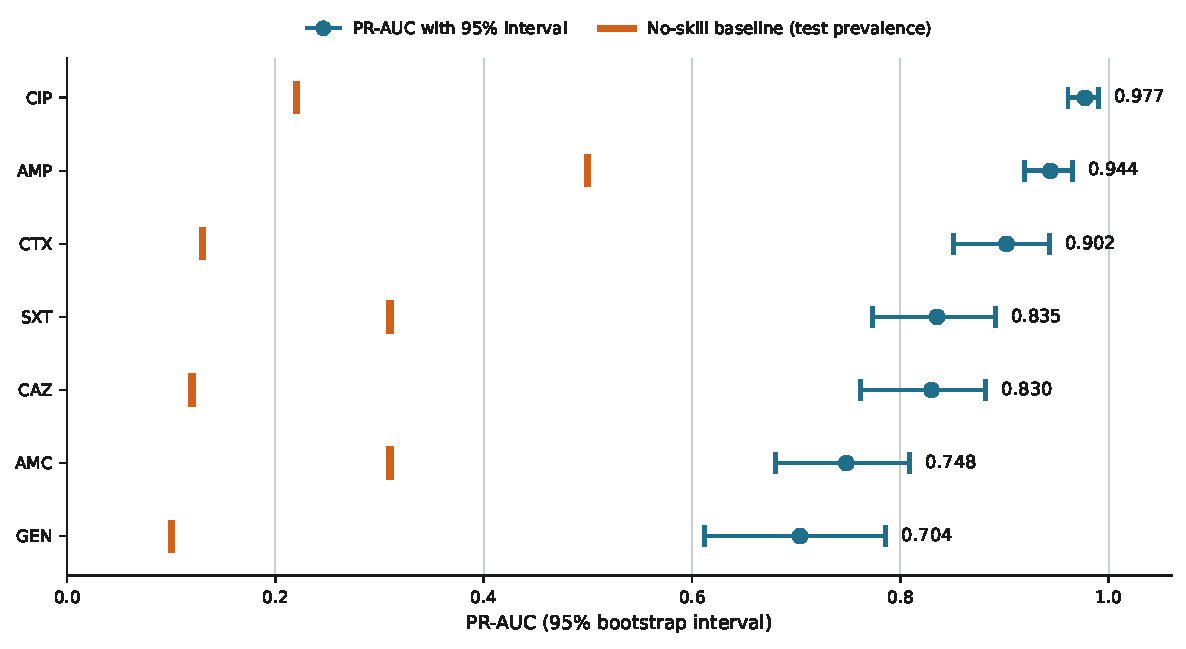
\includegraphics[width=\textwidth]{fig_ci_forest.pdf}
\caption{PR-AUC with 95\% bootstrap intervals, against each antibiotic's no-skill
baseline.}
\label{fig:ci_forest}
\fignote{The no-skill baseline is the test-set prevalence for that antibiotic.}
\end{figure}

\vspace{1em}

Table~\ref{tab:baselines} distinguishes between two similar but different
questions. The first is the comparison of the proposed model with external
models. There are three external baselines: a null model using only the
phylogroup label, TabNet and the gradient-boosting model using PCA components
that this project began with. The second question is what each component of the
proposed system contributes to the overall result. With this in mind, the five
base learners are tested individually as well. But these are not external
baselines. The proposed system consists of multiple learners, each feeding the
meta-learner. Thus, comparing these learners with the full system is not an
external comparison, but rather an ablation. All models were evaluated with the
same data splits and the same five-fold protocol. The values reported are the
mean PR-AUC scores of the seven antibiotics, and Figure~\ref{fig:baseline_ladder}
draws every row of the table on both splits at once.

\begin{table}[htb]
\centering
\caption{Comparisons of the proposed model with external baselines and results of
the component models. The phylogroup-only and PCA baselines were not evaluated
with the lineage holdout.}
\label{tab:baselines}
\small
\resizebox{\textwidth}{!}{%
\begin{tabular}{|l|r|r|}
\hline
\textbf{Model} & \textbf{PR-AUC, random split} & \textbf{PR-AUC, lineage holdout} \\ \hline
\multicolumn{3}{|l|}{\textit{External baselines}} \\ \hline
Phylogroup label only (null baseline) & 0.2914 & not run \\ \hline
TabNet, tabular deep learning baseline & 0.6951 & 0.3255 \\ \hline
XGBoost on 1{,}024 PCA components & 0.8033 & not run \\ \hline
\multicolumn{3}{|l|}{\textit{Components of the proposed system, each on its own}} \\ \hline
Random Forest, gene features & 0.7809 & 0.4931 \\ \hline
Logistic Regression, gene features & 0.7923 & 0.4408 \\ \hline
LightGBM, gene features & 0.8338 & 0.5516 \\ \hline
XGBoost, gene features & 0.8375 & 0.5507 \\ \hline
XGBoost, chi-squared filtered SNPs & 0.8400 & 0.6299 \\ \hline
\multicolumn{3}{|l|}{\textit{Proposed}} \\ \hline
\textbf{TriLens-MoE-Stack} & \textbf{0.8486} & \textbf{0.6337} \\ \hline
\end{tabular}
}
\vspace{0.4em}

\noindent\footnotesize\textit{Note:} The last row is the proposed model, the one every other row
in the table is being measured against.
\end{table}

\begin{figure}[htb]
\centering
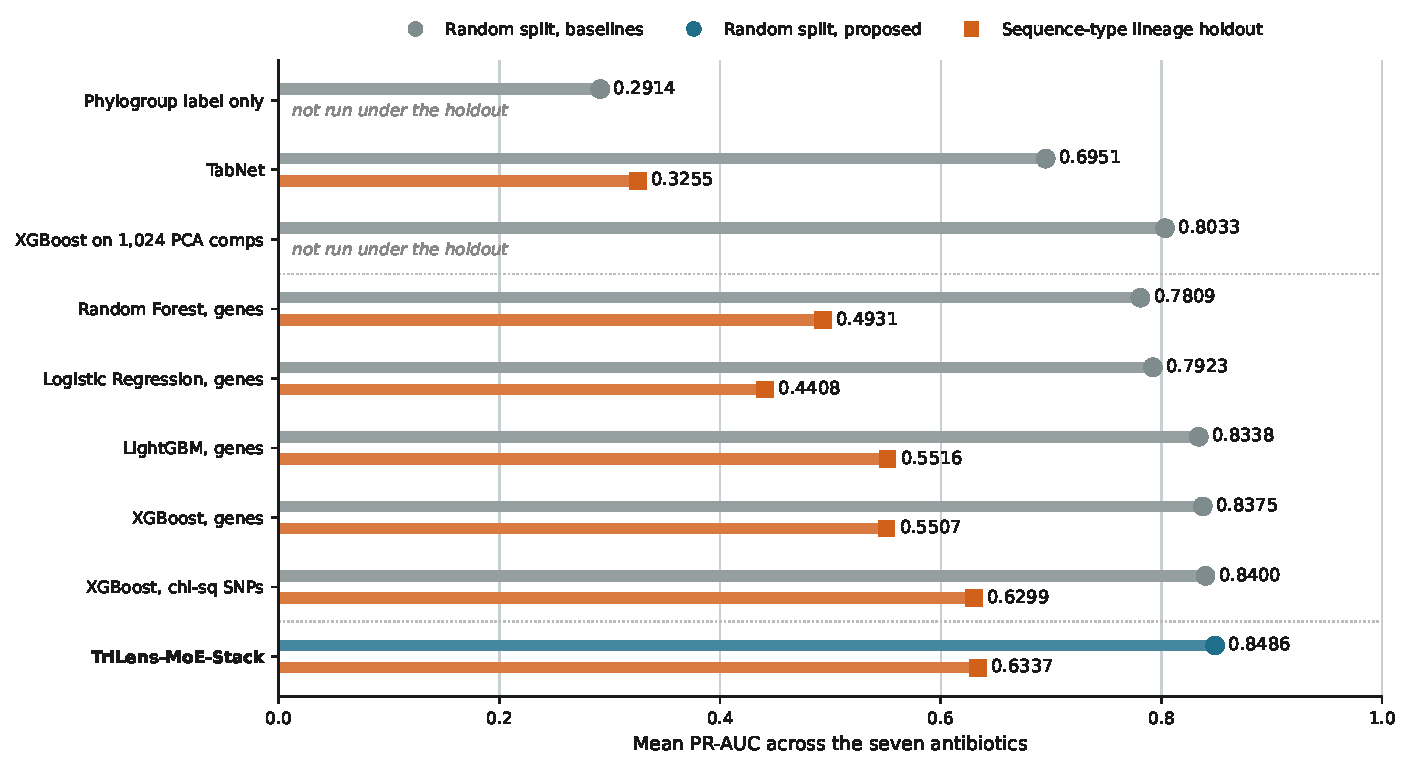
\includegraphics[width=\textwidth]{fig_baseline_ladder.pdf}
\caption{Every model of Table~\ref{tab:baselines} on both splits.}
\label{fig:baseline_ladder}
\fignote{The proposed model leads on the random split, but under the lineage holdout
the whole field compresses into a narrow band and the separation between methods
largely disappears.}
\end{figure}

On the random split the model produces the highest score of all entries in
the table. If only the eight-way phylogroup label is used as a baseline, the
PR-AUC reaches just 0.2914, almost equal to the average frequency of
resistance across the drugs, which is effectively the floor for this task.
The specialized tabular deep-learning baseline, TabNet, achieves only 0.6951,
behind every single classical learner, and falls to 0.3255 under the lineage
holdout, where even the weakest classical learner still reaches 0.4408: added
depth does not help on this problem under either test. The five classical
learners themselves range from PR-AUC 0.7809 to 0.8400, with the three
gradient-boosting models on the higher end of that span. The highest entry in the table, at 0.8486,
is TriLens-MoE-Stack, which leads every external baseline on the average and is ahead of
its own strongest component on five of the seven antibiotics. The
baselines are reported on PR-AUC as a single variable since this is what the
stacking pipeline reported about each learner when in isolation.

\vspace{1em}

It is not just the direction of the result that matters, but also the size of the
improvement. The proposed model outperforms the PCA baseline by 0.0453, TabNet by
0.1535 and the null model by 0.5572. The PCA comparison is the most telling as it
demonstrates what this project contributed, since this project began with the PCA
model. For individual antibiotics, the proposed model has scores above the upper
limit of the baseline interval for ampicillin, ciprofloxacin and
trimethoprim-sulfamethoxazole. Its score is within the interval for the other four
antibiotics. The greatest increase is for trimethoprim-sulfamethoxazole, which
goes from 0.7100 to 0.8352. But there is no benefit for amoxicillin-clavulanate.
This confirms the previous discovery that this is the antibiotic the model knows
the least about.

\vspace{1em}

The five base learners measure different things. The strongest learner gets 0.8400
by itself and the full system gets 0.8486. The difference is minimal at 0.009,
within the bootstrap intervals in Table~\ref{tab:ci}. This means that, as an
ablation result, the stacking layer provides a small improvement on top of the
best component. But this outcome does not mean that the system outperforms an
external method. A comparison of the full system with this component for each
antibiotic on each data split is provided in Table~\ref{tab:vsraw}.

\begin{table}[htb]
\centering
\caption{Comparison of the proposed model with its best single component, the
chi-squared filtered XGBoost, for each antibiotic. The antibiotics are sorted by
the gain on the random split.}
\label{tab:vsraw}
\small
\resizebox{\textwidth}{!}{%
\begin{tabular}{|l|r|r|r|r|r|r|}
\hline
& \multicolumn{3}{c|}{\textbf{Random split}} & \multicolumn{3}{c|}{\textbf{Lineage holdout}} \\ \hline
\textbf{Drug} & \textbf{XGB, $\chi^2$} & \textbf{Proposed} & \textbf{Gain} & \textbf{XGB, $\chi^2$} & \textbf{Proposed} & \textbf{Gain} \\ \hline
CAZ & 0.7951 & 0.8299 & $+0.035$ & 0.5180 & 0.4930 & $\mathbf{-0.025}$ \\ \hline
CTX & 0.8846 & 0.9019 & $+0.017$ & 0.6569 & 0.6073 & $\mathbf{-0.050}$ \\ \hline
SXT & 0.8183 & 0.8352 & $+0.017$ & 0.7609 & 0.7872 & $+0.026$ \\ \hline
AMP & 0.9432 & 0.9440 & $+0.001$ & 0.8910 & 0.9043 & $+0.013$ \\ \hline
CIP & 0.9770 & 0.9773 & $+0.000$ & 0.9348 & 0.9118 & $\mathbf{-0.023}$ \\ \hline
AMC & 0.7490 & 0.7482 & $\mathbf{-0.001}$ & 0.4704 & 0.4865 & $+0.016$ \\ \hline
GEN & 0.7128 & 0.7037 & $\mathbf{-0.009}$ & 0.1777 & 0.2457 & $+0.068$ \\ \hline
\textbf{Average} & \textbf{0.8400} & \textbf{0.8486} & $\mathbf{+0.009}$ & \textbf{0.6299} & \textbf{0.6337} & $\mathbf{+0.004}$ \\ \hline
\end{tabular}
}
\vspace{0.4em}

\noindent\footnotesize\textit{Note:} Bold marks the negative gains, where the full system loses
to its own best component: two drugs on the random split and three under the lineage holdout.
Every one of these differences is smaller than the bootstrap interval, so they indicate a
direction rather than a stable ranking.
\end{table}

The full system is more effective on five out of seven antibiotics on the random
split. The gain is more than 0.01 for three antibiotics: 0.035 for ceftazidime,
0.017 for cefotaxime, and 0.017 for trimethoprim-sulfamethoxazole. The difference
for ampicillin and ciprofloxacin is less than 0.001, meaning that they are
virtually the same. These antibiotics already have a score of 0.94 and 0.98 for
the single component, so there is not much room to improve. With the lineage
holdout the pattern changes. In this instance the entire system is more effective
against four antibiotics. Gentamicin has a gain of 0.068, the highest gain of any
individual antibiotic in this research. It is also the antibiotic on which the
single component has the lowest performance with a score of 0.1777. Ceftazidime
has the reverse trend. It gains most on the random split but it loses 0.025 under
the lineage holdout. All these individual differences are smaller than the
bootstrap interval. So they indicate the direction of the results, but do not
suggest a definite and stable ranking.

\vspace{1em}

The holdout column is a little less encouraging. The strongest single
classical learner reaches 0.6299 compared to 0.6337 for the full model, only a
gap of 0.004, but far less than the bootstrap uncertainty interval around
either value. This is the most unambiguous one-line answer to what this
research has discovered: none of the methods here stand out clearly from others
when lineage relatedness is not taken into account. Neither the ensemble nor
the hybrid design buys anything on unfamiliar strains, and all other analyses in
this chapter confirm this. This split was tested with TabNet, the only external
method. It had a score of 0.3255 and the overall system scored higher by 0.308.

This is one of the robustness checks that belong with these intervals. Some
bacterial collections have nearly identical strains. If one of the copies
ends up in training and the other ends up in the test set, the model may
score well on this task simply by recognizing something it has already seen,
so we checked for this reason. To assess this, we calculated the Hamming
distance from each test strain to its nearest training strain. The closest
pair differed by only 0.26\% of their SNP positions, and, out of 1{,}045 test
strains, 47 were within 0.5\% of a training strain, which are considered
``effectively duplicates.''

Then, we removed these 47 strains, and scored the model anew on the
remainder. PR-AUC decreased on average by 0.0041, with ceftazidime falling by
the largest, of 0.0209, and amoxicillin-clavulanate increasing by 0.0075. It
is very slight and not directional, which informs us that near-duplicates
will not be the primary factor that supports our findings. Nonetheless, it
remains a real effect and reporting the deduplicated number provides a
truthful lower bound.

\FloatBarrier
\section{Comparisons and Relationships}
\label{sec:comparisons}

\FloatBarrier
\subsection{Design Progression and the Tabular Deep Learning Baseline}

All of the major models we developed on the curated dataset are listed in
Table~\ref{tab:progression} in the order in which they were developed, and
Figure~\ref{fig:progression} draws the same sequence so the ceiling it runs into is
easier to see.

\begin{table}[htb]
\centering
\caption{Average PR-AUC across the seven antibiotics, for each stage of the
project on the curated dataset.}
\label{tab:progression}
\small
\begin{tabular}{|l|l|r|}
\hline
\textbf{Stage} & \textbf{Model} & \textbf{Avg PR-AUC} \\ \hline
Baseline            & XGBoost on 1{,}024 PCA components   & 0.8033 \\ \hline
Feature engineering & XGBoost on gene-level features   & 0.8297 \\ \hline
Single neural       & GeneAttentionNet v1              & 0.7430 \\ \hline
Single neural       & GeneAttentionNet v2 (best variant) & 0.7689 \\ \hline
Neural meta-stack   & Deep meta-learner variant        & 0.8253 \\ \hline
\textbf{Proposed}   & \textbf{TriLens-MoE-Stack}       & \textbf{0.8486} \\ \hline
\end{tabular}
\vspace{0.4em}

\noindent\footnotesize\textit{Note:} The delivered model reaches 0.8486, the ceiling every
earlier stage in this table, including a purely neural design, fell short of. Each row records
the score as it stood at that stage of the project, so the gene-feature XGBoost here is the
standalone run of the time and not the base learner of the same name inside the finished
pipeline, which Table~\ref{tab:baselines} reports at 0.8375.
\end{table}

\begin{figure}[htb]
\centering
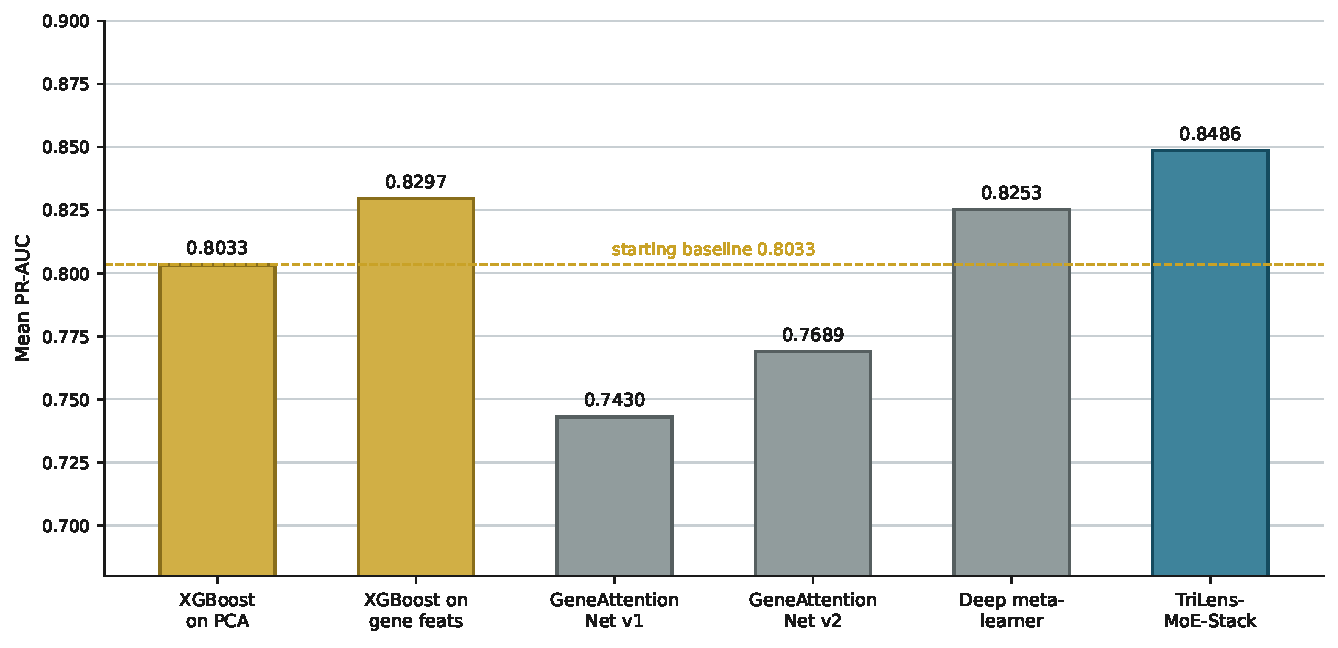
\includegraphics[width=\textwidth]{fig_progression.pdf}
\caption{The route to the final model, in the order the stages were built.}
\label{fig:progression}
\fignote{The two purely neural designs sit below the gradient-boosting baseline they
were meant to improve on, and the deeper meta-learner is worse than the simple one it
replaced. The vertical axis is truncated at 0.68 so that differences of a few
thousandths remain visible; no bar starts at zero.}
\end{figure}

The first true win came from features rather than models. Switching from PCA
components to gene-level features increased the score from 0.803 to 0.830 without
changing the learner at all, as aggregating variants per gene provided the model
with a biologically-meaningful input. Single neural models were disappointing:
GeneAttentionNet v1 only attained 0.743, worse than the plain XGBoost baseline,
and a second version only improved to 0.7689 after testing 7 design variants but
lost to XGBoost on all 7 antibiotics. It was the first clear indication we had
that purely neural approaches were not going to win here. At 0.8253, switching
from the logistic meta-learner to a deeper neural one made things worse. In fact,
taken as a whole, the table marks a ceiling: once the features were right,
none of our designs could go much beyond 0.85.

Because our neural lenses failed to outperform the classical learners, it would be
fair to ask us whether some other deep learning architecture would succeed.
Training TabNet, which is an architecture that targets tabular data, was done on
the same features with the same split, and Figure~\ref{fig:tabnet_vs_trilens} sets the
result beside the gradient-boosting baseline and our own model.

\begin{figure}[htb]
\centering
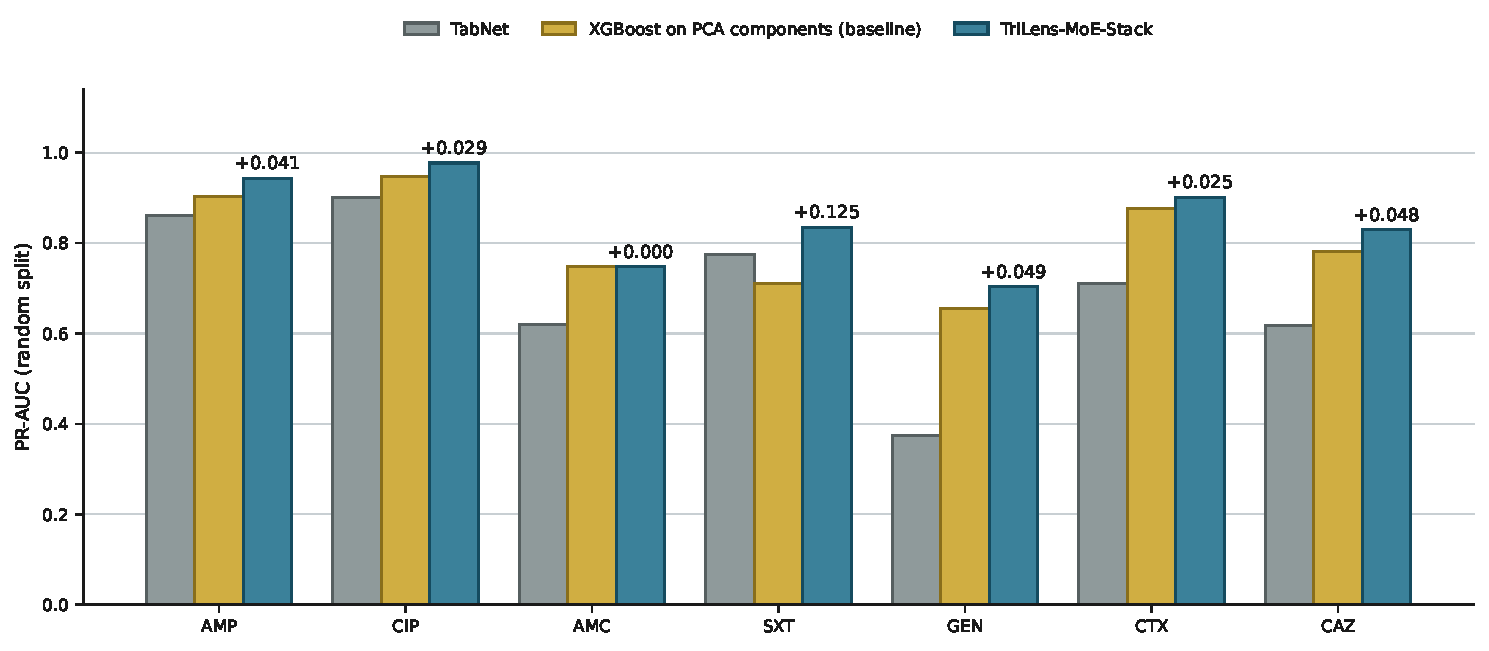
\includegraphics[width=\textwidth]{fig_tabnet_vs_trilens.pdf}
\caption{TabNet, the gradient-boosting baseline and TriLens-MoE-Stack, by antibiotic,
on the random split.}
\label{fig:tabnet_vs_trilens}
\fignote{The figure above each blue bar is the gain over the baseline, not over
TabNet.}
\end{figure}

The difference is large
and consistent. On each antibiotic individually, our model wins, on average by
0.154 (range, 0.061 on trimethoprim-sulfamethoxazole to 0.329 on gentamicin).
Consider gentamicin, the most clear-cut case; TabNet scored a mere 0.3751 on this
one when ours got 0.7037, and during training its validation score on that drug
swung between 0.58 and 0.80 from epoch to epoch and never settled. This does
not help establish the case of a general-purpose deep learning model for tabular
data alone, and both this comparison and the baseline ladder of
Table~\ref{tab:baselines} point in the same direction: it is the combination, not
the depth, that helps. The middle bar of each group is the gradient-boosting
baseline this project started from, and it tells a different story. That margin is
much smaller and far less even. It is widest on trimethoprim-sulfamethoxazole and
close to nothing on amoxicillin with clavulanic acid, where the baseline is
already almost as good as the finished model. A deep tabular model is not the
thing to beat here. The gradient-boosting baseline is.

\FloatBarrier
\subsection{The Lineage Holdout: Performance on Strains from Unseen Lineages}
\label{subsec:prevmatch}

The question posed in this subsection is more difficult: does the model
continue to work when it is presented with a strain it has never seen
before? The phylogroup-stratified split fails to do
it: it rearranges the information within eight large clusters, thus leaving a
strain and a close one on different sides, and its performance under it changes
little, between 0.849 and 0.853. This is not a test of unfamiliar strains, and
therefore could not have indicated a drop in any way.

The holdout which answers it makes use of the type of sequence of each strain, a
common designation of bacterial genetics according to which strains are clustered
by lineage. We successfully called a type of sequence to 6,487 of the 6,962
strains, or 93.2 per cent, with a total of 458 types, including a couple of giant
ones: sequence type 73 alone has 884 strains, or nearly one in every eight of the
samples. There were two rules prior to peeking at any outcome. Any strain whose
sequence type had no reliable sequence type was put into training and here, any
sequence type that comprised over five percent of the data was also put into
training, as a test set constructed using mostly a single clone would not be
testing generalisation. That condition was fulfilled by four types, namely, ST73,
ST131, ST95 and ST69. The other 454 sequences were assigned whole (not split),
using a fixed random seed such that no sequence type appears in more than one of
the training, validation and test sets.

The outcome was just the opposite. Mean performance plummets to 0.634 when they
are split by the lineage holdout, a decrease of over a fifth, and that is what the
phylogeny split had been unable to discover since it did not wipe any lineage off
training. Table~\ref{tab:mlst_per_ab} positions the three splits next to each
other.

\FloatBarrier
\begin{table}[htb]
\centering
\caption{Per-antibiotic PR-AUC under all three splits, with the drop measured from
the random split to the lineage holdout. Rows are ordered by that raw drop;
Figure~\ref{fig:lineage_drop} orders the same antibiotics by the
prevalence-corrected gap instead, which moves ciprofloxacin and
amoxicillin-clavulanate.}
\label{tab:mlst_per_ab}
\small
\begin{tabular}{|l|r|r|r|r|}
\hline
\textbf{Antibiotic} & \textbf{Random split} & \textbf{Phylogroup-strat.} & \textbf{Lineage holdout} & \textbf{Drop} \\ \hline
AMP & 0.9440 & 0.9338 & 0.9043 & $\mathbf{-0.040}$ \\ \hline
SXT & 0.8352 & 0.8373 & 0.7872 & $-0.048$ \\ \hline
CIP & 0.9773 & 0.9617 & 0.9118 & $-0.066$ \\ \hline
AMC & 0.7482 & 0.7963 & 0.4865 & $-0.262$ \\ \hline
CTX & 0.9019 & 0.8807 & 0.6073 & $-0.295$ \\ \hline
CAZ & 0.8299 & 0.8481 & 0.4930 & $-0.337$ \\ \hline
GEN & 0.7037 & 0.7136 & 0.2457 & $\mathbf{-0.458}$ \\ \hline
\textbf{Average} & \textbf{0.8486} & \textbf{0.8531} & \textbf{0.6337} & \\ \hline
\end{tabular}
\vspace{0.4em}

\noindent\footnotesize\textit{Note:} Ampicillin's drop of $-0.040$ is the smallest under the
lineage holdout and gentamicin's $-0.458$ the largest, the two-group pattern this chapter keeps
coming back to. Bold marks the extreme values in a column, best and worst alike.
\end{table}

\begin{figure}[htb]
  \centering
  \resizebox{\textwidth}{!}{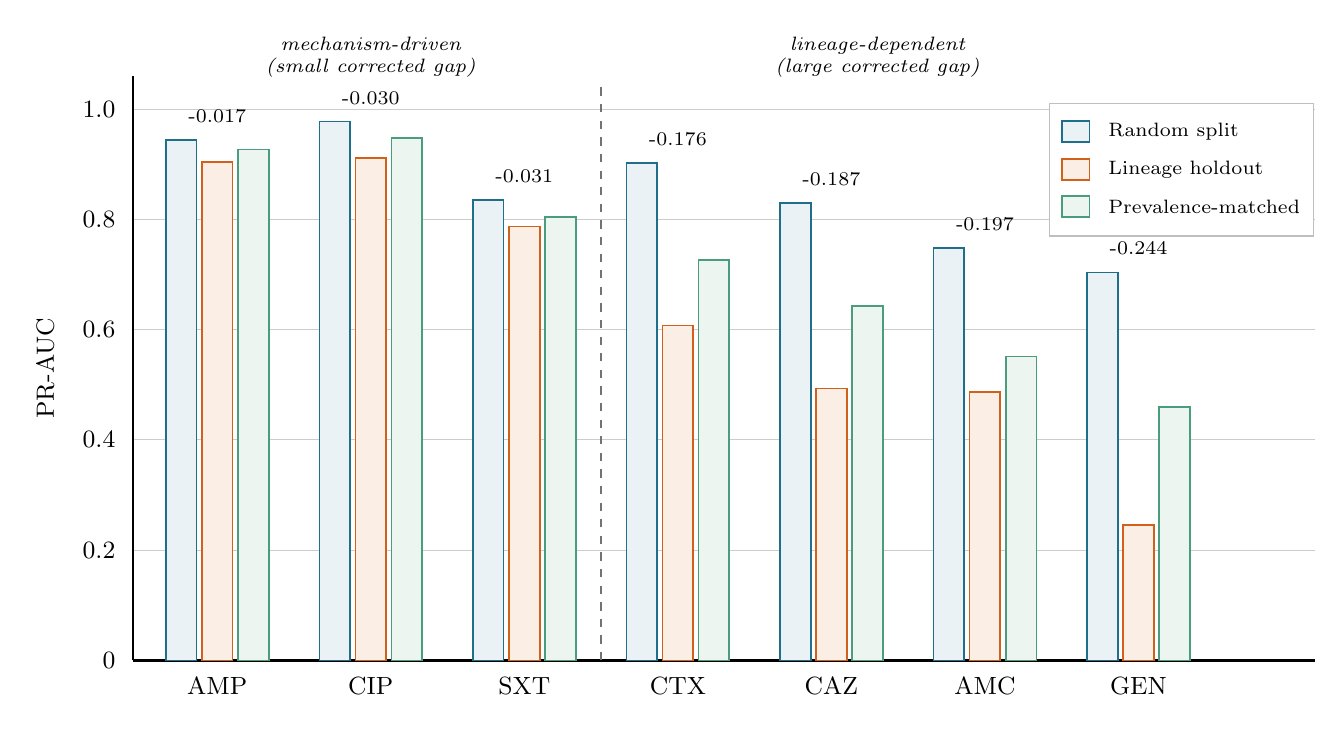
\begin{tikzpicture}[x=1.95cm, y=7.0cm]

\foreach \y in {0,0.2,0.4,0.6,0.8,1.0}{
  \draw[black!20,line width=0.4pt] (0.45,\y) -- (8.15,\y);
  \node[anchor=east,font=\small,text=black] at (0.40,\y) {\y};
}

\draw[black,line width=0.9pt] (0.45,0) -- (8.15,0);
\draw[black,line width=0.9pt] (0.45,0) -- (0.45,1.06);
\node[rotate=90,anchor=south,font=\small,text=black] at (0.00,0.53) {PR-AUC};

\foreach \i/\ab/\rnd/\hold/\mat/\gap in {%
  1/AMP/0.9440/0.9043/0.9268/{-0.017},
  2/CIP/0.9773/0.9118/0.9471/{-0.030},
  3/SXT/0.8352/0.7872/0.8046/{-0.031},
  4/CTX/0.9019/0.6073/0.7260/{-0.176},
  5/CAZ/0.8299/0.4930/0.6431/{-0.187},
  6/AMC/0.7482/0.4865/0.5513/{-0.197},
  7/GEN/0.7037/0.2457/0.4594/{-0.244}}{
    \fill[bluefill]  (\i-0.335,0) rectangle (\i-0.135,\rnd);
    \draw[blueedge,line width=0.6pt] (\i-0.335,0) rectangle (\i-0.135,\rnd);
    \fill[redfill]   (\i-0.10,0) rectangle (\i+0.10,\hold);
    \draw[rededge,line width=0.6pt] (\i-0.10,0) rectangle (\i+0.10,\hold);
    \fill[greenfill] (\i+0.135,0) rectangle (\i+0.335,\mat);
    \draw[greenedge,line width=0.6pt] (\i+0.135,0) rectangle (\i+0.335,\mat);
    \node[anchor=north,font=\small,text=black] at (\i,-0.014) {\ab};
    \node[anchor=south,font=\scriptsize,text=black] at (\i,\rnd+0.014) {\gap};
}

\draw[black!55,dashed,line width=0.8pt] (3.5,0) -- (3.5,1.04);
\node[anchor=south,font=\scriptsize\itshape,text=black,align=center]
  at (2.0,1.04) {mechanism-driven\\(small corrected gap)};
\node[anchor=south,font=\scriptsize\itshape,text=black,align=center]
  at (5.3,1.04) {lineage-dependent\\(large corrected gap)};

\fill[white] (6.42,0.770) rectangle (8.14,1.010);
\draw[black!25,line width=0.5pt] (6.42,0.770) rectangle (8.14,1.010);

\fill[bluefill] (6.50,0.940) rectangle (6.68,0.978);
\draw[blueedge,line width=0.6pt] (6.50,0.940) rectangle (6.68,0.978);
\node[anchor=west,font=\scriptsize,text=black] at (6.74,0.959) {Random split};

\fill[redfill] (6.50,0.872) rectangle (6.68,0.910);
\draw[rededge,line width=0.6pt] (6.50,0.872) rectangle (6.68,0.910);
\node[anchor=west,font=\scriptsize,text=black] at (6.74,0.891) {Lineage holdout};

\fill[greenfill] (6.50,0.804) rectangle (6.68,0.842);
\draw[greenedge,line width=0.6pt] (6.50,0.804) rectangle (6.68,0.842);
\node[anchor=west,font=\scriptsize,text=black] at (6.74,0.823) {Prevalence-matched};

\end{tikzpicture}
}
  \caption{Random split, the lineage holdout as measured, and the same holdout
  resampled to the training prevalence.}
  \label{fig:lineage_drop}
  \fignote{Bars are ordered by the prevalence-corrected gap, which is printed above
  each group, so the order differs from Table~\ref{tab:mlst_per_ab}, which is ordered
  by the raw drop. Three antibiotics lose 0.017 to 0.031 once prevalence is corrected
  for and four lose 0.176 to 0.244, with nothing in between. The values behind this
  figure are in Table~\ref{tab:previnv}.}
\end{figure}

The trend is not anywhere near homogenous and Figure~\ref{fig:lineage_drop}
renders the split apparent: three antibiotics struggle to move, four fall
sharply. Ampicillin has a loss of only 0.040 and gentamicin has a loss of 0.458.
It is the same ranking as in Sections~\ref{sec:perfeval} and~\ref{subsec:layerabl},
only much more emphatic here, since this is the first time a lineage has been
removed as opposed to reshuffled. The third bar in each group takes the
prevalence effect out, and the rest of this section explains what that means.

\vspace{1em}

There are two objections to be met before all this can be credited. One is that a
failure to generalise is not the only way a drop this large can occur,
it can also be caused by near-duplicate strains. On this split zero of the
1{,}045 test strains had a close match in training, using the same
nearest-neighbour scan described in Section~\ref{sec:statanalysis}, which found
47 such strains on the random split. The middle column of the table demonstrates this for the
phylogroup-stratified split: four antibiotics outperform the random split
and none declines by more than 0.022, which is not the behaviour of a split
that truly withholds a lineage. The second
objection does need correcting for: the holdout downwardly shifts the test-set
resistance prevalence for each antibiotic by between 2.5 and 12.1 percentage
points; gentamicin has only 38 resistant strains left. That has to be
distinguished from the drop before the drop can be interpreted as a loss of
skill.

\vspace{1em}

An unskilled classifier has an expected PR-AUC equal to the prevalence of the
positive class. This means that the whole scale on which PR-AUC is judged
moves with prevalence. A test partition containing fewer resistant strains
will therefore score lower even if the model ranks the strains in the same
order as before. We refer to this as the no-skill baseline rather than a
floor, because a poor enough classifier can still score below it. The
opposite extreme is gentamicin, with only 38 resistant
in its holdout test set, a prevalence of 4.2 percent as compared to 14.6 percent
in training.

\vspace{1em}

We directly measured the size of this effect. We repeatedly subsampled the
susceptible strains in the holdout test set to obtain the same prevalence as the
training set and recomputed PR-AUC on the same saved predictions for each
antibiotic. No model was re-trained and no resistant strain was abandoned.
Table~\ref{tab:previnv} presents mean over 2{,}000 resampling rounds with 95 per
cent interval and ROC-AUC with no-skill value of 0.5 irrespective of prevalence.

\FloatBarrier
\begin{table}[htb]
\centering
\caption{The lineage holdout with the prevalence effect removed. The
prevalence-matched column resamples the holdout test set to the training
prevalence; the final column is the resulting gap against the random split.}
\label{tab:previnv}
\small
\setlength{\tabcolsep}{4pt}
\begin{tabular}{|l|>{\raggedleft\arraybackslash}p{1.7cm}|>{\raggedleft\arraybackslash}p{2.0cm}|>{\raggedleft\arraybackslash}p{3.4cm}|>{\raggedleft\arraybackslash}p{1.6cm}|>{\raggedleft\arraybackslash}p{1.6cm}|}
\hline
\textbf{Antibiotic} & \textbf{Random split} & \textbf{Holdout, as measured} & \textbf{Holdout, prevalence-matched} & \textbf{ROC-AUC} & \textbf{True gap} \\ \hline
AMP & 0.9440 & 0.9043 & 0.9268 [0.918, 0.938] & 0.9257 & $\mathbf{-0.017}$ \\ \hline
CIP & 0.9773 & 0.9118 & 0.9471 [0.926, 0.967] & 0.9739 & $-0.030$ \\ \hline
SXT & 0.8352 & 0.7872 & 0.8046 [0.792, 0.823] & 0.9038 & $-0.031$ \\ \hline
CTX & 0.9019 & 0.6073 & 0.7260 [0.687, 0.766] & 0.8838 & $-0.176$ \\ \hline
CAZ & 0.8299 & 0.4930 & 0.6431 [0.600, 0.679] & 0.7878 & $-0.187$ \\ \hline
AMC & 0.7482 & 0.4865 & 0.5513 [0.529, 0.584] & 0.6894 & $-0.197$ \\ \hline
GEN & 0.7037 & 0.2457 & 0.4594 [0.398, 0.511] & 0.7426 & $\mathbf{-0.244}$ \\ \hline
\textbf{Average} & \textbf{0.8486} & \textbf{0.6337} & \textbf{0.7226} & \textbf{0.8439} & $\mathbf{-0.126}$ \\ \hline
\end{tabular}
\vspace{0.4em}

\noindent\footnotesize\textit{Note:} Once prevalence is corrected for, ampicillin's true gap is
$-0.017$, near nothing, against gentamicin's $-0.244$; the average true gap of $-0.126$ is still
well below the raw 0.215 gap the uncorrected numbers would suggest. Bold marks the extreme
values in a column, best and worst alike.
\end{table}

Only about two-fifths of the headline drop is a prevalence effect. Average
PR-AUC falls from 0.8486 (random split) to 0.7226 when prevalence is fixed, a
difference of 0.126, instead of 0.6337, a difference of 0.215, as the raw
holdout values would have indicated. As its own ROC-AUC of 0.7426 already
indicated, gentamicin is the one that most recovers, and its PR-AUC increases
from 0.2457 to 0.4594: the model had not ceased to rank resistant strains
above susceptible strains, it has merely been forced to do so on a test set
where only one in twenty-four strains is resistant.

Adjusting the prevalence does not remove the discovery, instead it clarifies
it. The seven antibiotics remain divided into the same two categories, but
even more distant relative to each other. Ampicillin, ciprofloxacin and
trimethoprim-sulfamethoxazole have a loss of 0.017 to 0.031 in PR-AUC, which
is near nothing, and cefotaxime, ceftazidime, amoxicillin-clavulanate and
gentamicin have a loss of 0.176 to 0.244, and no antibiotic is in between. A
model that had merely deteriorated on a more challenging set of tests would
exhibit an even distribution of losses among all seven drugs rather than this
two group divide. Amoxicillin-clavulanate is the cleanest: its prevalence
changes only by 5.9 points, thus it recovers the least of the four hard drugs
(a PR-AUC increase of 0.065, compared to gentamicin's 0.214) and also has the
lowest ROC-AUC of all seven, at 0.6894, so the least of its loss can be
attributed to prevalence at all.

Two caveats apply to this table. First, gentamicin's prevalence-matched
interval is wide, [0.398, 0.511], because it is anchored by only 38 resistant
strains, so its exact value should be read with caution even though its
direction is clear. Second, the holdout prevalence used for matching is the
\textit{training} prevalence, which is slightly higher than the random-split
test set's prevalence; this makes the comparison somewhat generous to the
holdout, so the true gap may be a little larger than the 0.126 reported
above.

\vspace{1em}

What the holdout costs in clinical terms is the next question.
Section~\ref{sec:perfeval} reported clinical error rates on the random split. Of
greater interest is what happens to the errors that get to a patient if the
strain is from an unfamiliar lineage. Table~\ref{tab:holdoutclin} does, using the
same saved predictions and the same fixed threshold of 0.5, and
Figure~\ref{fig:clinical_heatmap} does the same with the numbers arranged by
severity.

\FloatBarrier
\begin{table}[htb]
\centering
\caption{Clinical error rates under the lineage holdout against the random split,
at a threshold of 0.5. Being within-class ratios, VME and ME are unaffected by the
prevalence shift. Rows are ordered by holdout VME, the same order as
Figure~\ref{fig:clinical_heatmap}.}
\label{tab:holdoutclin}
\small
\setlength{\tabcolsep}{4pt}
\resizebox{\textwidth}{!}{%
\begin{tabular}{|l|>{\raggedleft\arraybackslash}p{1.7cm}|>{\raggedleft\arraybackslash}p{1.3cm}|>{\raggedleft\arraybackslash}p{1.3cm}|>{\raggedleft\arraybackslash}p{1.5cm}|>{\raggedleft\arraybackslash}p{1.3cm}|>{\raggedleft\arraybackslash}p{1.3cm}|>{\raggedleft\arraybackslash}p{1.3cm}|>{\raggedleft\arraybackslash}p{1.3cm}|}
\hline
\textbf{Antibiotic} & \textbf{Resistant in test} & \textbf{VME random} & \textbf{VME holdout} & \textbf{Increase} & \textbf{ME random} & \textbf{ME holdout} & \textbf{CA random} & \textbf{CA holdout} \\ \hline
CIP & 132 & 0.086 & 0.114 & $+0.028$ & 0.015 & 0.006 & 0.969 & 0.978 \\ \hline
AMP & 300 & 0.109 & 0.160 & $+0.051$ & 0.104 & 0.095 & 0.893 & 0.877 \\ \hline
SXT & 142 & 0.236 & 0.310 & $+0.074$ & 0.080 & 0.072 & 0.871 & 0.863 \\ \hline
AMC & 145 & 0.394 & 0.710 & $+0.316$ & 0.108 & 0.076 & 0.804 & 0.754 \\ \hline
CAZ & 43  & 0.291 & \textbf{0.837} & $+0.546$ & 0.033 & 0.001 & 0.936 & 0.959 \\ \hline
GEN & 38  & 0.436 & \textbf{0.868} & $+0.432$ & 0.023 & 0.002 & 0.934 & 0.962 \\ \hline
CTX & 71  & 0.190 & \textbf{0.915} & $+0.725$ & 0.026 & 0.001 & 0.953 & 0.918 \\ \hline
\textbf{Mean} & & \textbf{0.249} & \textbf{0.559} & $\mathbf{+0.310}$ & \textbf{0.056} & \textbf{0.036} & & \\ \hline
\end{tabular}
}
\vspace{0.4em}

\noindent\footnotesize\textit{Note:} Gentamicin (0.868), ceftazidime (0.837) and cefotaxime
(0.915) all have a holdout VME above 0.83, meaning the model has effectively stopped finding
resistance for these three; the mean row averages across all seven.
\end{table}

\begin{figure}[htb]
\centering
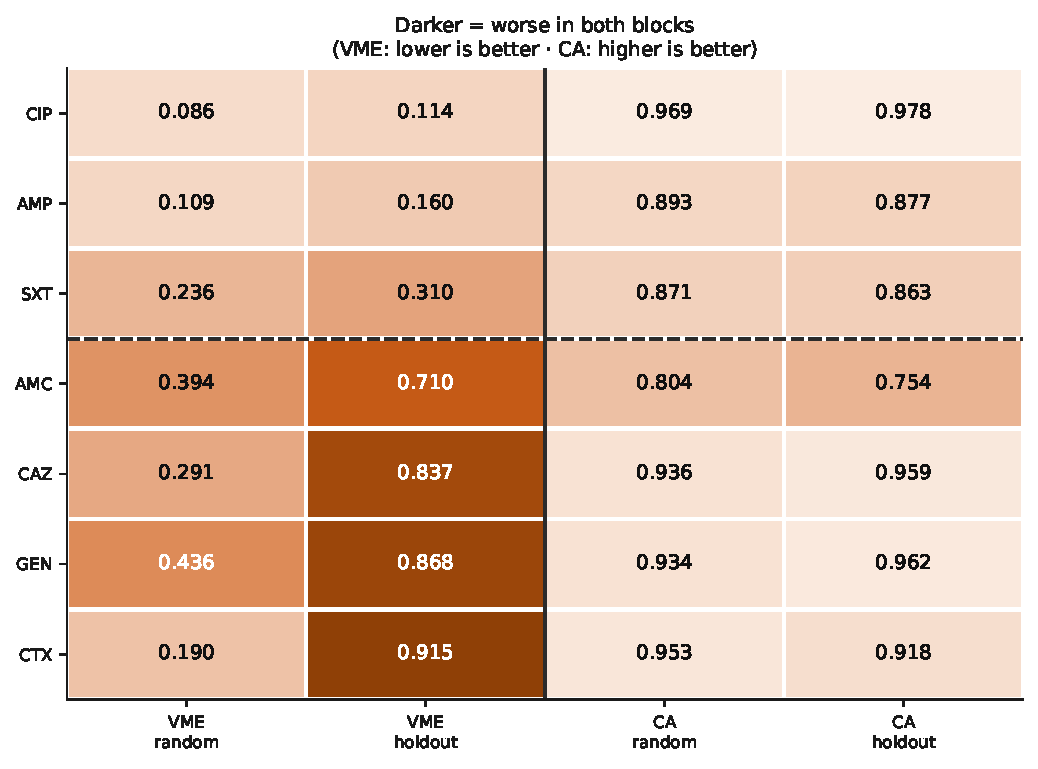
\includegraphics[width=\textwidth]{fig_clinical_heatmap.pdf}
\caption{Very major error rate and categorical agreement, random split against
lineage holdout.}
\label{fig:clinical_heatmap}
\fignote{Both blocks use a single scale on which a darker cell is the worse result.
The categorical-agreement columns are shaded by $1-\mathrm{CA}$ so that the
convention holds throughout. Drugs are ordered by holdout very major error rate; the
dashed line marks the split between the two groups.}
\end{figure}

The average very major error rate increases from 0.249 to 0.559 and for three
antibiotics, the model has completely ceased to detect resistance. It detects
6 of the 71 cefotaxime-resistant strains, 5 of the 38
gentamicin-resistant strains and 7 of the 43 ceftazidime-resistant strains, with a
major error rate of 0.001 or 0.002 for each group. That combination is the
hallmark of a classifier that has collapsed onto the
majority class: it hardly ever makes a resistant prediction, so it hardly ever
makes such predictions wrongly. These numbers are more difficult to dispute
than the PR-AUC values above since VME and ME are calculated within a class and
stay fixed as the class mix varies. Prevalence-matching resamples only
susceptible strains, and very major error rate is considered to be all in the
resistant category, thus cannot be resampled. Clinical deterioration here
therefore has no prevalence component, and requires no correction before it can
be believed.

The categorical agreement column demonstrates why accuracy does not drive this
research. Three antibiotics show equal or higher categorical agreement in the
holdout than in the random split, and for the other four the reduction in
agreement is much smaller than the total collapse in clinical safety alongside
it. Gentamicin increases from 0.934 to 0.962 while very major error rate doubles
to 0.868; ceftazidime from 0.936 to 0.959, missing 36 of the 43 resistant
strains; cefotaxime changes by just 0.035 but its very major error rate rises from
0.190 to 0.915. By the measure a machine learning paper would use to report
results, this model looks better or nearly as good, on unseen lineages; by the
measure a clinician would use, it became unusable.

This is the third analysis to produce the same grouping. They are the same three
with the same saved predictions and test set, therefore they are complementary
views but measure different aspects of those predictions. The three antibiotics
with negligible loss in PR-AUC gain between 0.028 and 0.074 in very major error
rate, and the four with a significant loss have a gain of 0.316 to 0.725. The
order within the second group changes, as cefotaxime is worst in this group
whereas gentamicin was worst using PR-AUC, the rank within the groups is not to be
overly read, but the grouping, which is based on the drug's performance in the
corresponding group, does not change across all three analyses.

The holdout also allows us to redo the component analysis of
Section~\ref{subsec:layerabl} in more difficult conditions, and
Table~\ref{tab:mlst_components} shows that the outcome alters the previous
picture.

\FloatBarrier
\begin{table}[htb]
\centering
\caption{Average PR-AUC of each component of the model, under the lineage
holdout.}
\label{tab:mlst_components}
\small
\begin{tabular}{|l|r|}
\hline
\textbf{Component} & \textbf{Avg PR-AUC} \\ \hline
TriLens neural arm alone (lenses with gate) & 0.472 \\ \hline
Five classical learners alone & \textbf{0.628} \\ \hline
Full hybrid model & \textbf{0.634} \\ \hline
\end{tabular}
\vspace{0.4em}

\noindent\footnotesize\textit{Note:} The classical learners alone reach 0.628, close to the full
hybrid model's 0.634 under this harder split, meaning the neural lenses add almost nothing here.
The 0.634 in the last row is the 0.6337 reported to four decimal places in
Table~\ref{tab:mlst_per_ab}. The 0.628 in the middle row is the five base
learners \emph{stacked}, and is a different quantity from the 0.6299 of
Table~\ref{tab:vsraw}, which is the single strongest learner on its own: under
this split the stacking layer recovers slightly less than its own best member
already had.
\end{table}

The neural arm alone, that is the three lenses with the gate, scored 0.781 on the
random split (Section~\ref{subsec:layerabl}). It plummets to 0.472 here, when tested on truly
unseen lineages; this represented a much larger decline compared to what the
classical learners achieve on their own (0.628), nearly matching the full hybrid
model (0.634). The classical learners do nearly all of the work under a true test
of generalisation and the neural lenses add almost nothing. It is a stronger
form of what Section~\ref{subsec:layerabl} already indicated: the gap between
the two arms is 0.156, and the fused model only
recovers 0.006 of it. But this was not a case where some other deep learning
design would have generalised better; TabNet reran on this split averages 0.326,
worse than our neural lenses on their own and well below the classical learners.
Gradient-boosted trees on gene-level features are the best method we identified
on this dataset and under this type of test.

\vspace{1em}

The downside on unseen lineages gives one an obvious next question: does it work
at all on a different set of strains? The two datasets do not have a shared
feature vector as Arcadia uses the pan-genome reference with 535{,}000 variant
positions and Giessen uses a single reference with approximately 60{,}000
variant positions. We rather trained the classical stacking part of the pipeline
on Giessen with the same protocol and hyperparameters. The three neural lenses
require feature shapes only the pan-genome view can provide and thus are not
included in this comparison; and four antibiotics are in common to both
collections. The Giessen collection is summarised in Figure~\ref{fig:giessen_overview}
prior to the reporting of how well the classical stack transfers to it in
Table~\ref{tab:giessen_transfer}, with Figure~\ref{fig:giessen_retention} setting the
rebuilt scores beside their Arcadia counterparts.

\FloatBarrier
\begin{figure}[htb]
\centering
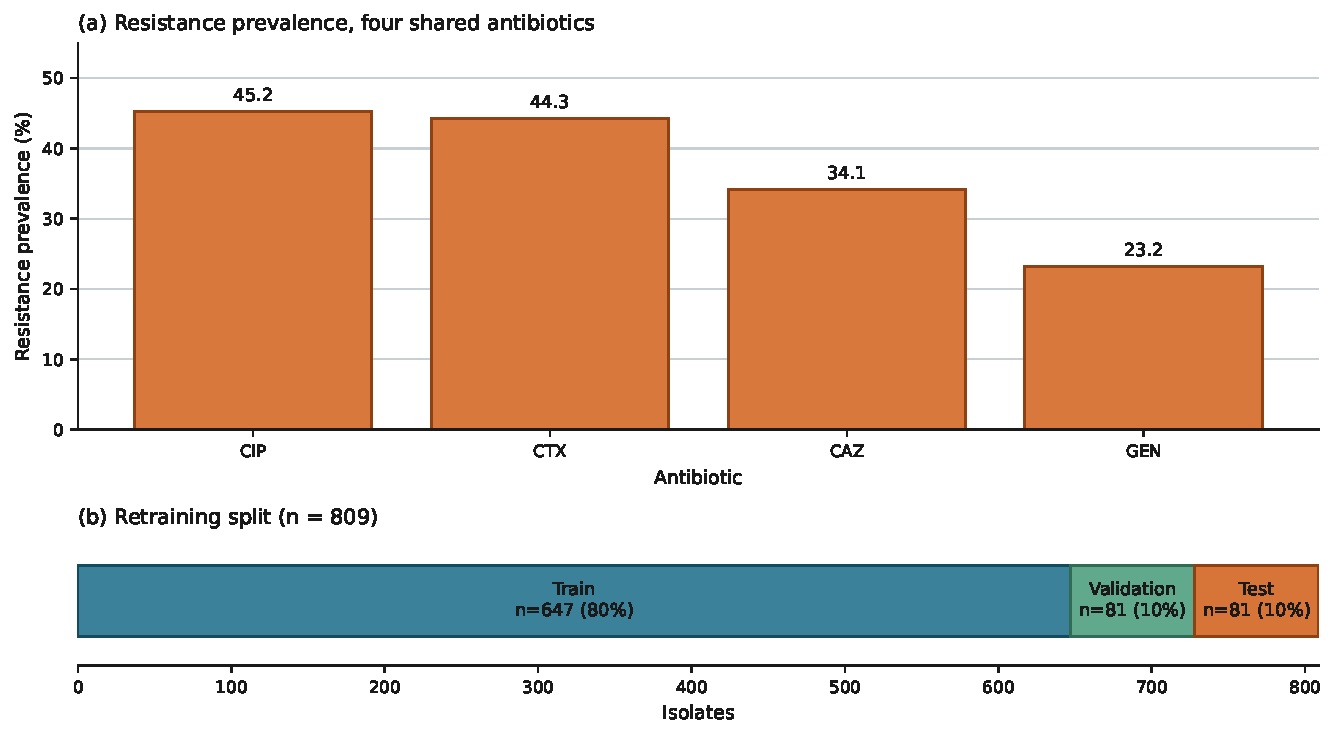
\includegraphics[width=\textwidth]{fig_giessen_overview.pdf}
\caption{The Giessen set: resistance prevalence and the retraining split.}
\label{fig:giessen_overview}
\fignote{\textbf{(a)} Resistance prevalence for the four shared antibiotics.
\textbf{(b)} The 647/81/81 retraining split (n = 809). Every isolate here carries a
label for all four antibiotics, so nothing is missing.}
\end{figure}

\begin{table}[htb]
\centering
\caption{The classical stacking half of the pipeline, trained independently on a
second collection. Neither column is the full TriLens model.}
\label{tab:giessen_transfer}
\small
\begin{tabular}{|l|r|r|r|}
\hline
\textbf{Antibiotic} & \textbf{Arcadia} & \textbf{Giessen} & \textbf{Retention} \\ \hline
CIP & 0.9773 & 0.9868 & \textbf{101.0\%} \\ \hline
CAZ & 0.8299 & 0.7775 & 93.7\% \\ \hline
CTX & 0.9019 & 0.7876 & 87.3\% \\ \hline
GEN & 0.7037 & 0.5480 & \textbf{77.9\%} \\ \hline
\textbf{Average} & \textbf{0.8532} & \textbf{0.7750} & \textbf{90.0\%} \\ \hline
\end{tabular}
\vspace{0.4em}

\noindent\footnotesize\textit{Note:} Ciprofloxacin's apparent 101.0\% retention is the highest in
the table and gentamicin's 77.9\% the lowest, matching the ordering seen under the lineage
holdout. As the text below explains, these retention figures are inflated by Giessen's higher
prevalence rather than by genuinely better performance. Bold marks the extreme values in a
column, best and worst alike.
\end{table}

\begin{figure}[htb]
\centering
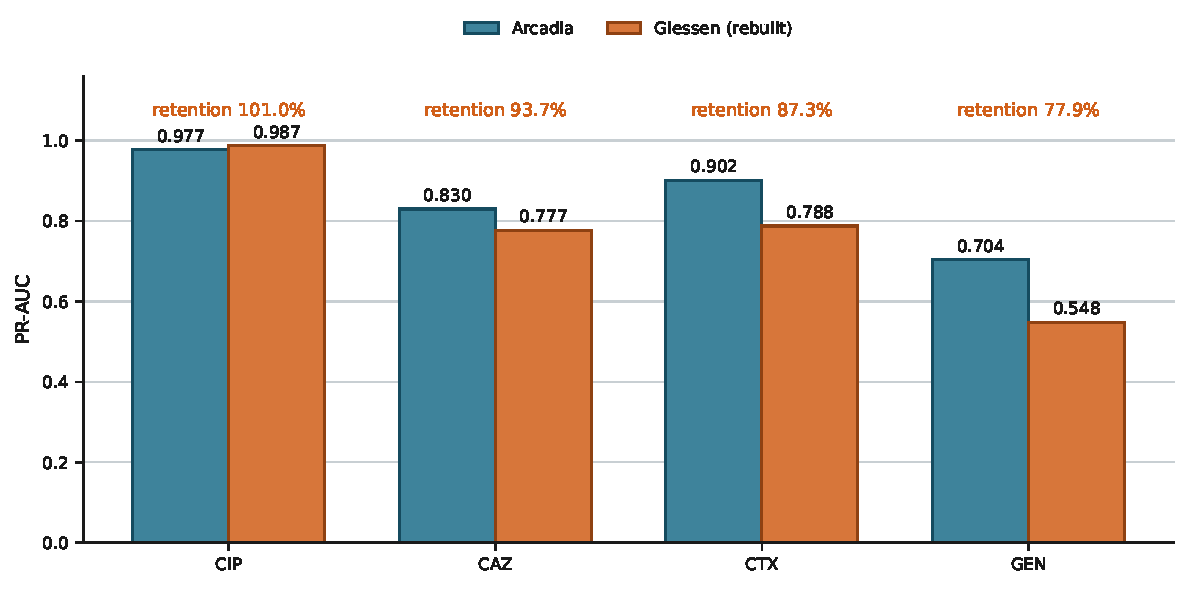
\includegraphics[width=\textwidth]{fig_giessen_retention.pdf}
\caption{The classical stack rebuilt on the Giessen collection, against its Arcadia
scores.}
\label{fig:giessen_retention}
\fignote{Ciprofloxacin transfers almost intact while gentamicin retains least, the
same ordering the lineage holdout produces. The retention figures are inflated by
Giessen's higher prevalence, as the text below explains.}
\end{figure}

The approach keeps about 90\% of its performance on a genomically different
collection. It is not zero-shot transfer, in that the model was retrained; what
it demonstrates is that our design decisions are not optimized to the specifics
of a single dataset.

\vspace{1em}

There is one caveat here, the same one this chapter raises so many times
elsewhere. Section~\ref{subsec:prevmatch} holds that PR-AUC cannot be compared
across partitions with differing prevalence, and the two collections differ
significantly in prevalence. In Arcadia, the resistance of ciprofloxacin
stands at 0.228 as compared to 0.452 in Giessen. Cefotaxime is 0.152 resistant
in Arcadia as compared to 0.443 in Giessen. In Arcadia, ceftazidime is 0.131
resistant against 0.341 in Giessen. Gentamicin has a resistance of 0.118 in
Arcadia compared to 0.232 in Giessen. In Giessen, every drug's no-skill
baseline is about twice to three times Arcadia's, before the model is
credited with any skill at all. So the
retention percentages are misleading by this difference in baselines, not by any
actual improvement, and perhaps the most transparent example is ciprofloxacin
whose apparent 101\% indicates that the model is marginally better on Giessen,
but what really happened is that Giessen made the task marginally easier. The
bias cannot be eradicated, because prevalence-matching would require both
collections to be resampled to an identical reference, and the 81-strain Giessen
test partition is too small to survive that exercise. The weaker argument is the
one we will justify from this table: that the recipe reconstructs and does not
fall apart, not that performance is maintained to within ten percent of its
original extent. The interesting part is the per-antibiotic pattern.
Ciprofloxacin retains most of its performance and gentamicin only 77.9\% of its
own, the same order as under the lineage holdout, though reached by an entirely
different route.

\FloatBarrier
\subsection{Comparison with Published Work on the Same Dataset}
\label{subsec:published}

The group that originally released our dataset subsequently published its own
analysis of the same strains \cite{york2025amr}. That gives us a rare chance
to independently audit our results against theirs. The two studies count different
things, so cannot be directly compared with the numbers they produce, nor ours.
Arcadia applied a Bayesian sparse linear mixed model fit to the complete dataset
and reported \emph{heritability}, a measure of the proportion of the variance in
a trait that can be attributed to genetic variation among individuals, while we
trained a classifier and reported PR-AUC (area under the precision-recall curve)
on an independent test set, a measure of the classifier's ability to predict
strains it has not previously seen; a trait may be highly heritable but, at the
same time, difficult to predict on new samples. They also investigated three
antibiotics against our seven and 7{,}043 strains as opposed to our 6{,}962.
What we can compare are the results, and there the agreement is remarkable
despite very different approaches. Table~\ref{tab:arcadia} sets the two accounts
side by side.

\begin{table}[htb]
\centering
\caption{Our findings against the published analysis of the same dataset. The two
studies report different measures, so only the biological conclusions are
compared.}
\label{tab:arcadia}
\small
\begin{tabular}{|>{\raggedright\arraybackslash}p{3.3cm}|>{\raggedright\arraybackslash}p{5.3cm}|>{\raggedright\arraybackslash}p{5.3cm}|}
\hline
\textbf{Topic} & \textbf{Arcadia analysis \cite{york2025amr}} & \textbf{This work} \\ \hline
Driver of ciprofloxacin resistance &
Three linked mutations: two in \textit{gyrA} and one in \textit{parC} &
\textbf{\textit{gyrA} and \textit{parC} appear among our top marker genes} \\ \hline
Driver of ampicillin resistance &
Plasmid and transposon fragments, led by a TEM-1 beta-lactamase &
A beta-lactamase gene appears among our markers \\ \hline
Driver of trimethoprim-sulfamethoxazole resistance &
No interpretable resistance locus could be identified &
No resistance gene was found for this antibiotic either \\ \hline
Reason some resistance genes are hard to find &
The pan-genome is fragmented, so plasmid-borne genes assemble poorly &
The same explanation fits our weak results for GEN and AMC \\ \hline
\end{tabular}
\vspace{0.4em}

\noindent\footnotesize\textit{Note:} The ciprofloxacin row is the strongest agreement in the
table: an independent team's mutation-level finding and our model's gene-level finding point to
the same two genes, \textit{gyrA} and \textit{parC}.
\end{table}

There are three rows that should be commented on. Our ciprofloxacin match is most
powerful: Arcadia had discovered three mutations each, at distinct locations in
\textit{gyrA} and \textit{parC}, whereas our model, which never received that
information, discovered the two genes by itself based on SHAP values on the
classical learners. The same outcome of trimethoprim-sulfamethoxazole is
interesting due to the opposite reason. Arcadia could not associate their best
markers with any known resistance mechanism and neither could we; they observed
that its best markers indicated aminoglycoside-related proteins, which have
nothing to do with this drug, and took on the hypothesis that the actual
resistance gene is located on a poorly assembled fragment of a plasmid on which
its best markers just happen to be situated. There was no other reasonable
explanation and it is heartening that, a specialist team also arrived at the
identical dead-end. Of particular importance to our discussion is the fragmented
pan-genome point, which, as Section~\ref{sec:discussion} indicates, is part of
the reason that gentamicin and amoxicillin-clavulanate do not work well, namely,
the fact that their resistance genes are carried on plasmids and transposons that
are not cleanly represented here. Arcadia came up with the same conclusion on a
different axis on their own and this gives us greater assurance that it must be
in the representation of data and not in our model.

There is one other number to discuss. The heritability values estimated by
Arcadia showed that the genetic markers in this dataset explain nearly all of the
variation between resistant and susceptible strains: 0.99 for ciprofloxacin, 0.95
for ampicillin and 0.94 for trimethoprim-sulfamethoxazole. The same three
antibiotics with the same values of PR-AUC on the random-split test set were 0.9773,
0.9440 and 0.8352; thus, ciprofloxacin is not far off what the heritability
suggests is possible, while trimethoprim-sulfamethoxazole is clearly behind.
Although the two sets of numbers are not directly comparable, the pattern is
informative: if the signal is nearly fully present in the markers, that limit of
$\sim$0.85 that all models in Table~\ref{tab:progression} reached is unlikely to be a
biological limit and more likely a limit of how the features are built. As stated
in Section~\ref{subsec:layerabl}, increased model complexity adds little and the
heritability estimates indicate the same trend from the other side. The missing
performance is not in a larger network, but in a better assembly, where the genes
of the plasmid and the transposon are no longer broken up and can be represented
as a complete gene.

\FloatBarrier
\subsection{Comparing Two Collections: The Cause of the Convolutional Network's Failure}
\label{subsec:cnnfail}

This section returns to the open question left by Section~\ref{subsec:ownprep}. Our initial
experiments with the 1D CNN were not successful, which led us to propose that the issue was
structural rather than a matter of tuning. A convolutional network learns local patterns from
adjacent positions, so if it is really learning from local structure, scrambling the order of the
input columns should destroy its performance, and leave it unchanged if the order never mattered.
The naive 1D CNN averaged 0.4826 on Arcadia against 0.6889 on Giessen, a difference of 0.2063,
but that gap proves nothing on its own, since the two collections differ in prevalence, labelling
standard and size. The shuffle test settles it by comparing each collection against itself.
Rerunning ciprofloxacin with the SNP columns shuffled, the two behaved in opposite ways: Giessen
declined from 0.8635 to 0.5411, a loss of 0.322, while Arcadia moved from 0.7473 to 0.7957 and so
gained a little. Where destroying the order raises the score, the model was not using order in the
first place. Table~\ref{tab:locality} sets out both halves of the test.

\begin{table}[htb]
\centering
\caption{The locality test. Panel (a) is the naive one-dimensional CNN trained
separately on each collection; panel (b) reruns ciprofloxacin with the SNP column
order permuted, a separate retraining run, which is why its ordered Giessen score
differs slightly from panel (a). All values are test PR-AUC, 95 per cent bootstrap
intervals in brackets.}
\label{tab:locality}
\small
\begin{tabular}{|l|c|c|r|}
\hline
\multicolumn{4}{|l|}{\textbf{(a) Naive 1D CNN, per antibiotic}} \\ \hline
\textbf{Antibiotic} & \textbf{Arcadia} & \textbf{Giessen} & \textbf{Gap} \\
                    & \textit{(pan-genome)} & \textit{(single reference)} & \\ \hline
CIP & 0.7473 & 0.8559 & $+0.109$ \\ \hline
CTX & 0.5107 & 0.8343 & $+0.324$ \\ \hline
CAZ & 0.3802 & 0.7535 & $+0.373$ \\ \hline
GEN & 0.2921 & 0.3117 & $+0.020$ \\ \hline
\textbf{Average} & \textbf{0.4826} & \textbf{0.6889} & $\mathbf{+0.206}$ \\ \hline
\end{tabular}

\vspace{1em}

\begin{tabular}{|l|c|c|r|}
\hline
\multicolumn{4}{|l|}{\textbf{(b) Ciprofloxacin with the SNP column order shuffled}} \\ \hline
\textbf{Collection} & \textbf{Ordered} & \textbf{Shuffled} & \textbf{Effect} \\ \hline
Giessen \textit{(single reference)} & 0.8635 & 0.5411 & $\mathbf{-0.322}$ \\
                                    & \footnotesize[0.781, 0.928]
                                    & \footnotesize[0.416, 0.668] & \\ \hline
Arcadia \textit{(pan-genome)}       & 0.7473 & 0.7957 & $+0.048$ \\
                                    & \footnotesize[0.682, 0.809]
                                    & \footnotesize[0.745, 0.843] & \\ \hline
\end{tabular}
\vspace{0.4em}

\noindent\footnotesize\textit{Note:} On Giessen the ordered and shuffled intervals do
not overlap and the shuffled model's MCC falls from 0.469 to 0.000, collapsing to
calling every strain resistant. On Arcadia the intervals overlap and the point estimate
moves \emph{upwards}, so there was no positional signal to destroy. That asymmetry is
the evidence for confining convolution to gene blocks.
\end{table}

The asymmetry can be explained by the way the two datasets are constructed. Giessen maps all strains
to one reference genome, so column 100 and column 101 really are adjacent locations on the same
chromosome. Arcadia employs a pan-genome reassembling a large number of strains, so two adjacent
columns may contain different contigs, different genes, or even different portions of the accessory
genome altogether, and there is no local structure to be sought. Lens A therefore convolves only
within each gene block, where positions are genuinely adjacent, and pools across genes with attention.

\FloatBarrier
\section{Discussion}
\label{sec:discussion}

The above results lead to a question which transcends model comparison. We find our model
reasonably predictive of resistance on familiar strains but the question of greater interest is
what it is actually learning to make such predictions, and how much of that survives on strains it
has never seen.

\FloatBarrier
\subsection{The Genes the Model Relies On}
\label{subsec:attnfix}

We obtained the most impactful genes based on two sources: the weights of attention within the
three neural lenses, and SHAP values obtained with the five classical base learners. This provided
1{,}138 marker genes in total which covered all antibiotics. Their prokka locus tags alone do not
provide us with any information, so we aligned them with the eggNOG functional annotation released
with the Arcadia dataset. We were successful in annotating 889 of the 1{,}138 markers, or 78.1\%,
with the others having no corresponding match and indicating them as not annotated instead of
making a best guess. Eight of the annotated markers were known genes involved in antimicrobial
resistance: gyrA, parC, the two target genes where point mutations result in fluoroquinolone
resistance; emrB, mdtC, mdtD, mdtO and cusA, which are parts of multidrug efflux pumps, and one
additional gene annotated as a beta-lactamase.

The genuine result is in finding gyrA and parC and it is more significant following the lineage
holdout than ever. These are the textbook objectives of ciprofloxacin resistance and ciprofloxacin
was the very antibiotic that did not succumb to the holdout most, dropping only 0.030 when
prevalence is held constant, as compared to other antibiotics that dropped up to 0.244. A model
based on an actual, conceptually clear mutation should be transferred to a new lineage and that is
what we observe. One detail, though, is more important than the list of genes. The eight resistance genes were all the
result of the SHAP analysis of the classical learners. None was a result of attention weights of
the three neural lenses, although, 420 out of the 1{,}138 markers were selected out of those
lenses.

\vspace{1em}

Two things besides a real failure could bring about that zero, and we tested each of them. The first is annotation coverage, as an eggNOG file lacks a gene and there is no
way to identify it as a resistance gene no matter how significant the model considered it to be.
The two of three lenses are eliminated by coverage: each of 140 markers contained in the
Cross-Antibiotic Context Module was annotated, and 97.9\% of markers in the Motif Pattern Encoder,
but neither generated a single resistance gene. The weaker case is the Gene Feature Attention
Module at 61.4\%, which is important as it is the lens the gate is most dependent on, thus the
view that our model believes is best will be the one that we can reasonably interpret least. The
second option is that twenty genes per lens per drug is too small a window and we did the
annotation in the top 100 genes five times, increasing coverage to 79.3\%. It also did not
reproduce any resistance gene, hence it is not an artefact of the position at which the list was
broken as well.

Another measurement can be used to explain why. The variant sweep that followed the final lens
design concentrated focus on the 5{,}000 selected genes instead of the entire catalogue of
32{,}441 genes, thus the maximum attainable entropy there was $\ln 5{,}000 \approx 8.52$, not the
$\ln 32{,}441 \approx 10.39$ of the full set. Compared against this lower ceiling, attention
entropy remains at 8.51 for trimethoprim-sulfamethoxazole, effectively at ceiling, and above 7.79
for amoxicillin-clavulanate, gentamicin, cefotaxime and ceftazidime, still at or within ten percent
of it. When the attention mass of the five drugs is at the most not even one percent of the total
mass, in any case, and when ninety percent of it is distributed amongst two or four thousand
genes, the pooling layer has virtually broken down into a mere mean. Only ampicillin and
ciprofloxacin exhibit real concentration, with entropies 5.34 and 5.46 with just under twenty
genes exceeding one percent each, and we by no means attribute biology to even that, since another
pooling function tested in a separate sweep concentrated on another group of drugs, indicating the
pattern follows the architecture and not the resistance mechanism.

\vspace{1em}

What it does focus on is still informative. Each gene in the pan genome has a locus
tag that indicates which of the assemblies the gene was called from, providing an inexpensive
method to determine which of the attended genes are sampled or from across the pan genome. For the
Gene Feature Attention Module they are not: for each of the 7 antibiotics, the top genes by this
module were concentrated in a single assembly between 12 times that assembly's fraction in the
catalogue and 23 times: median was 16.4. Those counts are less informative because they represent a
small number of genes per antibiotic, only genes with an assembly tag can be counted and that
counts less than a dozen genes in total, so we read the ratio more as an indicator of the direction
of the lens than as a formal test.

An obvious objection is that this is simply an artefact of how pan-genome clusters are named, as
each cluster takes the tag of whichever assembly represented it, and a well represented assembly
would then swamp any list by arithmetic. There are two reasons why not to think so. The assembly
the lens focuses on provides merely 3.3\% of the catalogue, therefore abundance cannot account
for a sixteen-fold preference. And the other two lenses do only just what the artefact explanation
would predict: both focus on the \textit{most} populous tag they are reading, at an enrichment of
only 1.6 to 2.1, so that we do not report them as a discovery. The natural interpretation of that
enrichment, then, is that the lens has learnt a lineage fingerprint,
i.e. genes that are expected to be transmitted along a branch of the population will indeed be
transmitted along the same branch of the population. We attempted to test this rather than simply
assuming it was right. The reading does not hold: as Table~\ref{tab:umark} later in this section
shows, the attended genes are \emph{less} lineage-determined than a randomly chosen gene, not
more.

\vspace{1em}

These above are what attention still cannot do. They are, however, much better than the results
obtained via a direct application of gated attention pooling on this input, and this difference is
one of the design contributions of this work: it is the only area where we changed the mechanism
itself rather than the data it reads from. Section~\ref{subsec:lensB} and
Equations~\eqref{eq:expertB_ctx}--\eqref{eq:expertB_score} set out the argument in full: on a
presence-and-absence vector the standard gated-attention score becomes simply that gene's
embedding, and is thus identical for all strains that carry that gene, and conditioning it on the
mean embedding of the genes the strain actually carries restores per-sample behaviour. As this
reasoning predicts a behaviour, we evaluated it in an ablation, training the model in both
directions using the same seeds, folds, splits and hyperparameters, changing only this single
term. Table~\ref{tab:attnfix} reports the effect.

{\small
\setlength{\tabcolsep}{4pt}
\setlength{\LTpost}{0pt}
\begin{longtable}{|>{\raggedright\arraybackslash}p{7.6cm}|>{\centering\arraybackslash}p{2.0cm}|>{\centering\arraybackslash}p{2.2cm}|>{\centering\arraybackslash}p{1.9cm}|}
\caption{Ablation of strain conditioning in the Gene Feature Attention Module.
Only this term differs; the second column is the delivered model.}
\label{tab:attnfix}\\
\hline
\textbf{Measure} & \textbf{Standard} & \textbf{Strain-cond. (delivered)} & \textbf{Change} \\
\hline
\endfirsthead
\hline
\textbf{Measure} & \textbf{Standard} & \textbf{Strain-cond. (delivered)} & \textbf{Change} \\
\hline
\endhead
\hline
\multicolumn{4}{r}{\footnotesize\textit{Continued on the next page}}\\
\endfoot
\hline
\endlastfoot
\multicolumn{4}{|l|}{\textit{Predictive performance}} \\ \hline
Random split, full stack & 0.8462 & 0.8486 & $+0.0024$ \\ \hline
Phylogroup-stratified split & 0.8519 & 0.8531 & $+0.0012$ \\ \hline
Lineage holdout, full stack & 0.6300 & 0.6337 & $+0.0037$ \\ \hline
Lineage holdout, classical learners only & 0.628 & 0.628 & $\pm 0$ \\ \hline
\textbf{Lineage holdout, neural lenses alone} & \textbf{0.437} & \textbf{0.472} & $\mathbf{+0.035}$ \\ \hline
\multicolumn{4}{|l|}{\textit{Where the performance comes from (random split)}} \\ \hline
Stage 1, three lenses averaged & 0.7324 & 0.7453 & $+0.0129$ \\ \hline
Stage 2, plus the mixture-of-experts gate & 0.7547 & 0.7807 & $+0.0260$ \\ \hline
Contribution of the gate & $+0.0224$ & $\mathbf{+0.0353}$ & N/A \\ \hline
Contribution of classical stacking & $+0.0914$ & $+0.0679$ & N/A \\ \hline
\multicolumn{4}{|l|}{\textit{Clinical safety (random split, threshold 0.5)}} \\ \hline
Mean very major error rate & 0.257 & 0.249 & $-0.008$ \\ \hline
Antibiotics inside both CLSI limits & 0 of 7 & 0 of 7 & N/A \\ \hline
\multicolumn{4}{|l|}{\textit{Interpretability}} \\ \hline
Resistance genes recovered by attention & 0 & \textbf{1} & N/A \\ \hline
$U_{res}$ of the attended genes & 0.0192 & \textbf{0.0419} & $+0.0227$ \\ \hline
$U_{ST}$ of the attended genes & 0.3123 & 0.3569 & $+0.0446$ \\ \hline
Enrichment on a single assembly & $16.4\times$ & $9.0\times$ & N/A \\ \hline
Distinct source assemblies among top genes & 13 & 25 & N/A \\ \hline
\end{longtable}}
\vspace{-0.8em}

\noindent\footnotesize\textit{Note:} Under the lineage holdout the neural lenses alone gain 0.035
against 0.0024 on the random split, and the interpretability rows move with it. SHAP reaches
$U_{res}=0.0473$ and a random gene set $U_{ST}=0.5390$ (Table~\ref{tab:umark}); ``N/A'' marks
rows where a change is not meaningful.\normalsize

One caveat applies to every attention figure in this section, and it is worth stating precisely
so that the reader knows what these weights describe. The predictions and the gate weights
reported elsewhere are averaged across the five cross-validation folds, so each of those numbers
reflects the ensemble as a whole. The attention arrays are not. The training loop writes them
only at the end of the final fold, so every attention figure and every attention-derived count
in this section describes one of the five models behind the scores rather than their average.
The five folds share the same architecture, the same seed and the same feature set, and differ
only in which portion of the training data was held out, so we would expect their attention
patterns to be broadly similar. We cannot demonstrate that from the saved output, however, and
we would rather record the limitation than assume it away. It is an artefact of how the training
loop writes its results rather than a decision about method, and because it applies equally to
the standard and the strain-conditioned runs, the comparison between the two columns of
Table~\ref{tab:attnfix} is not affected by it.

\vspace{1em}

All the interpretability measures go in the expected direction, and
Figure~\ref{fig:attention_concentration} shows the clearest of them, the weight the lens
places on its top-ranked genes before and after the change.

\begin{figure}[htb]
\centering
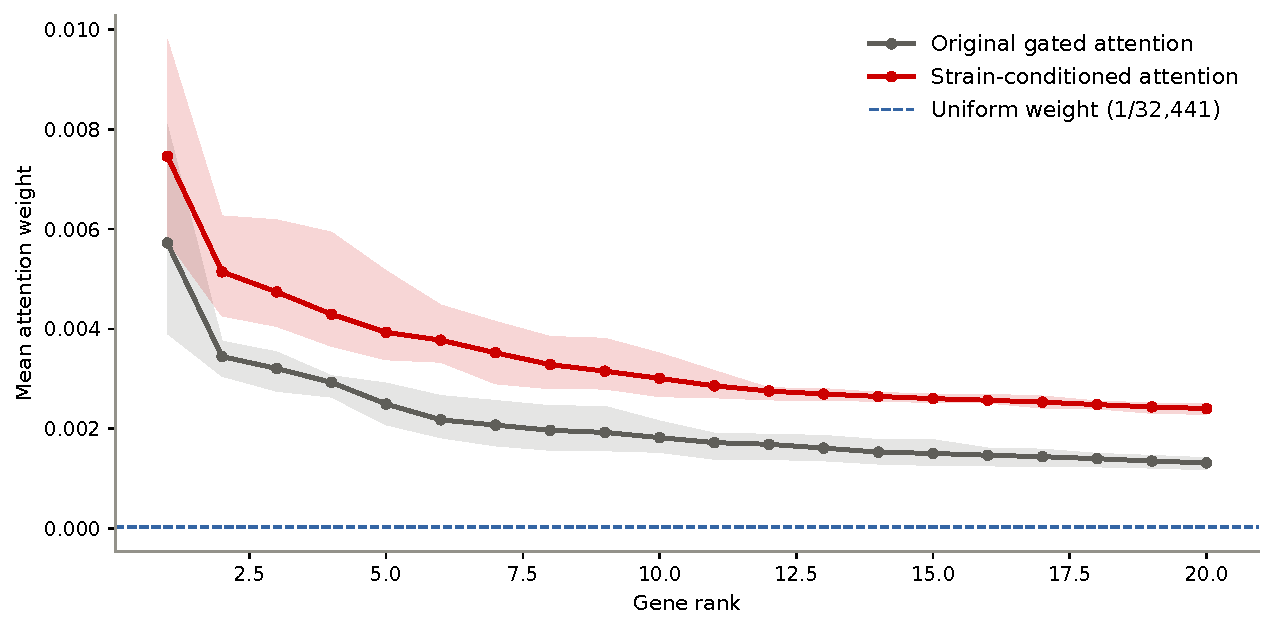
\includegraphics[width=\textwidth]{fig_attention_concentration.pdf}
\caption{Mean attention weight against gene rank in the Gene Feature Attention
Module, before and after strain conditioning.}
\label{fig:attention_concentration}
\fignote{Averaged over the seven antibiotics; the band is the range across them and
the dashed line is uniform weight over all 32{,}441 genes. The strain-conditioned
lens weights its top-ranked genes more heavily, the change
Table~\ref{tab:attnfix} records as $U_{res}$ rising from 0.0192 to 0.0419.}
\end{figure}

The strain-conditioned lens
concentrates more weight on its highest-ranked genes at every rank, and the
resistance information of the
attended genes more than doubles from 0.0192 to 0.0419, which is 89\% of the SHAP-selected genes
on average, and greater than them on five out of seven antibiotics. The focus on a
single assembly drops from 16.4-fold to 9.0-fold and three out of the seven drugs are no longer
significant in the 5\% threshold and the number of independent source assemblies between the
attended genes almost doubles, and as a result the provenance signature is mostly diluted.

\vspace{1em}

The rows of performance are not as plain as they appear at the first sight as the term buys
practically nothing where it can be measured with ease and much where it is needed. Strain conditioning is
worth almost nothing where it is easiest to measure: $+0.0024$ on the random split, and
$+0.0037$ on the full stack under the lineage holdout. It is worth an order of magnitude more,
$+0.035$, on the neural lenses alone under that same holdout, while the classical learners do
not move at all and stay at 0.628. An ablation run only on the random split would have hidden
this completely. The degenerate scoring function was costing the neural arm most of what it
lost anywhere, on precisely the split this research is interested in, and the classical arm was
strong enough that none of that loss ever showed in the headline number. Section~\ref{subsec:prevmatch}, which argues that
the classical learners carry most of this model's performance, therefore survives a version in
which the neural side is meaningfully better, a stronger form of the same argument.

\vspace{1em}

The term also changes the division of the work in the model. The gate contributes $+0.0224$
against the stacking step's $+0.0914$, a ratio of four to one; and $+0.0353$ against $+0.0679$, a
ratio of two to one. There was no change in ordering and all the antibiotics continued to improve
monotonically throughout the three stages, but about half the perceived difference between the
neural and classical halves was the result of a scoring function that was not strain-dependent.
Clinical appearance changes hardly at all: the average very major error value is reduced from
0.257 to 0.249 and the major error value is the same at three decimal places, and no antibiotic can fall
within both CLSI limits. Whatever this term is worth, it is not the reason the model is
clinically unusable.

\vspace{1em}

Our most interesting change is the one which we have not tuned for. The attention restores
MFCAOJAD\_04226, a beta-lactamase, with the score conditioned to the presence of the
strain, and selectively recovers it with ampicillin and amoxicillin-clavulanate, the two
penicillins in our panel and the two drugs which a beta-lactamase can explain being resistant to.
It is the locus tag that SHAP had already determined in the classical learners and thus, two
attribution paths that previously disagreed on all points now converge on a single gene,
independently. We do not exaggerate this: it is a single gene per hundred genes tested each lens
per drug, it is ranked 19 and 20 instead of first, and \textit{gyrA} and \textit{parC} have not
appeared in the attention rankings. It does not mean that this lens can be interpreted, since the
findings in the previous section demonstrate that, it cannot. The argument is that the standard
formulation could not have been, however much else was amiss, and that the difference can be
traced to one term in the scoring function.

\vspace{1em}

One boundary applies. This is information on the presence and absence vector for attention, and
is specific to that input, not to attention pooling in general. What generalises is that the
diagnostic is an attention mechanism whose scores do not change across samples, which means that
we cannot obtain a per-sample explanation and we can figure out that fact in minutes, without
retraining anything, from the entropy and information checks in this section. We computed the
fraction of presence-absence entropy, $U_{ST}(g) = I(g;\mathrm{ST})/H(g)$, which is equal to 1 if
a gene's presence is completely attributed to its lineage and 0 if it says nothing about the
gene's lineage. In Table~\ref{tab:umark} the selected genes are compared with the genes attended
and to 500 random selections of equal size, and Figure~\ref{fig:lineage_marker} draws the two
measures side by side.

\begin{table}[htb]
\centering
\caption{How much of each gene set is explained by lineage ($U_{ST}$) and by
resistance ($U_{res}$), over the top twenty genes per antibiotic. The attention row
is the standard formulation; the delivered strain-conditioned lens reaches 0.357
and 0.0419.}
\label{tab:umark}
\small
\begin{tabular}{|>{\raggedright\arraybackslash}p{5.6cm}|r|r|r|r|}
\hline
\textbf{Gene set} & \textbf{$U_{ST}$} & \textbf{vs.\ random} & \textbf{$U_{res}$} & \textbf{vs.\ attention} \\ \hline
Random genes (500 draws) & 0.539 & N/A & N/A & N/A \\ \hline
SHAP, classical learners & 0.375 & $0.70\times$ & \textbf{0.0473} & $2.5\times$ \\ \hline
Attention, Gene Feature Attention Module & \textbf{0.312} & $0.58\times$ & \textbf{0.0192} & N/A \\ \hline
\end{tabular}
\vspace{0.4em}

\noindent\footnotesize\textit{Note:} Attention's $U_{ST}$ of 0.312 is lower than a random gene's
0.539, so the attended genes are not a lineage marker; its $U_{res}$ of 0.0192 is less than half
of SHAP's 0.0473, so they carry far less resistance information than the genes the classical
learners select.
\end{table}

\begin{figure}[htb]
\centering
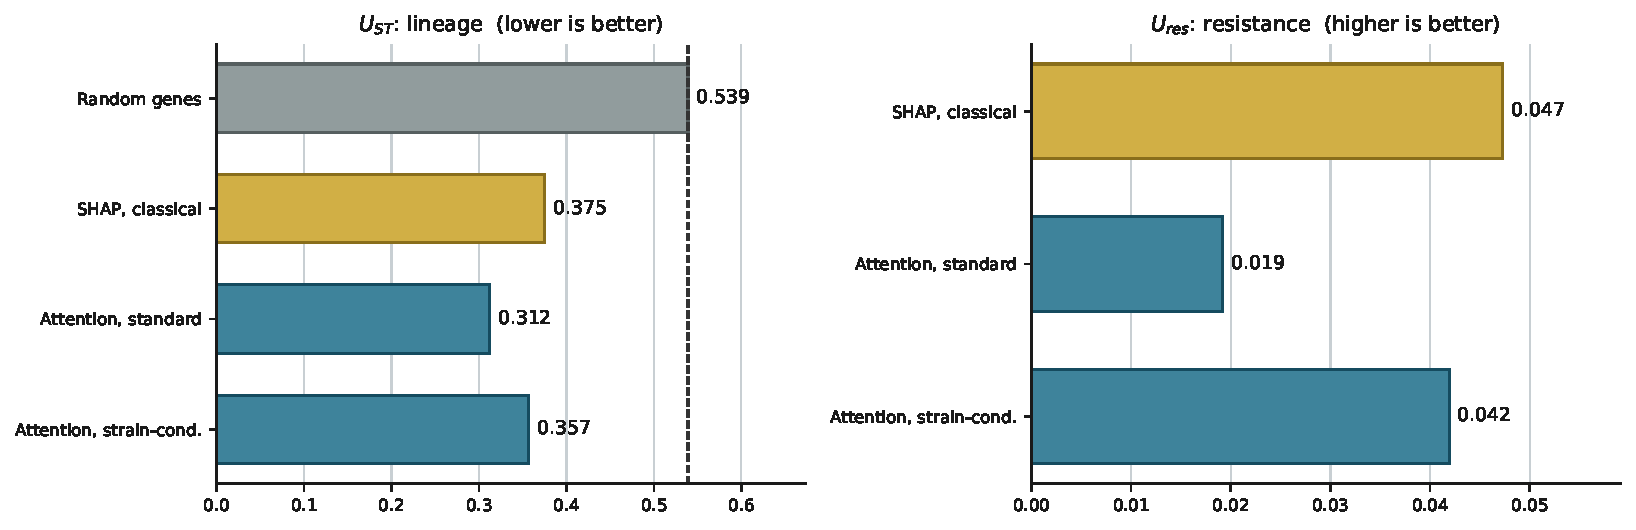
\includegraphics[width=\textwidth]{fig_lineage_marker.pdf}
\caption{The attended gene sets against SHAP on both measures.}
\label{fig:lineage_marker}
\fignote{Random draws appear on the lineage measure only, since a random gene set has
no resistance value to compare against. Lower is better on the left, higher is better
on the right.}
\end{figure}

There are two things that follow, both depicted in Figure~\ref{fig:lineage_marker}. The first is
not a feature of our model itself, but of the data: the presence-absence pattern of a random gene
from this pan-genome is explained to 54\% by sequence type. Such strongly lineage-structured
content of \textit{E. coli} accessory genes is the most obvious single reason why a
lineage-sensitive split was required in the first place.

\vspace{1em}

The second one is that the genes attended are not a lineage marker. They are \textit{less}
determined by lineage than a random gene, at 0.312 under the standard formulation and 0.357
under the delivered one, and nothing in the 500 random draws fell below them. Nor do they hold
much information of resistance: their $U_{res}$ of 0.0192 in Table~\ref{tab:umark} is the lowest
of the three sets, about half the 0.0473 that the genes SHAP chooses do, and even the
strain-conditioned version is only 0.0419. It is not the lens that read the wrong thing but the
lens that read hardly anything. Its focus is nearly even with five of the seven drugs; where it
focuses, it focuses on genes that share a provenance that does not predict either lineage or
resistance; and none of the resistance genes is in its rankings at any window we tested. The
useful part is the comparison with SHAP in that, both sets of genes were selected on the same
trained pipeline on the same features: the classical side picks genes with two and a half times
more resistance information. This matches the result reported in Section~\ref{subsec:prevmatch},
where the neural lenses alone under the lineage holdout remain at 0.472 while the classical learners
remain at 0.628. It is the same learners who generalise that are also the ones which pick the more
informative genes.

\vspace{1em}

This conflict does not exist solely on the neural side. In the classical arm, the two attribution
modes also struggle to agree to a great degree. When the top twenty genes ranked by XGBoost gain
are compared with the top twenty genes ranked by SHAP, by each antibiotic and by both sets of
classical features, the Jaccard overlap ranges between 0.053 and 0.212, with an average of 0.11 on
the gene-aggregated features and 0.17 on the raw SNP features, so at best only four to six genes
out of twenty will be shared between the two lists. The rank correlation is not so good: Spearman
is negative with all seven antibiotics, between $-0.04$ and $-0.53$. The results of two methods of
attributing to the same trained model are not expected to differ this much and hence neither can
be taken as the interpretation of the model itself. The findings of the gene level, then, are
reported as leads but not settled biology, such as the eight resistance genes above, which are
informative because they are all in agreement with independently determined biology but not
because the attribution method has ascertained them.

\FloatBarrier
\subsection{Population Structure and the Mistakes Behind the Lineage Split}

Prior to running the lineage holdout, we checked a simpler question first: the accuracy of
resistance predictions from a model able to predict from nothing but each strain's broad
phylogroup, limited to an 8-way label with no genomic context whatsoever.
Table~\ref{tab:phylogroup} reports what that baseline achieves.

\begin{table}[htb]
\centering
\caption{A baseline given only the eight-way phylogroup label, with no genomic
features, against the proposed model on the random split.}
\label{tab:phylogroup}
\small
\begin{tabular}{|l|r|r|}
\hline
\textbf{Antibiotic} & \textbf{Phylogroup only} & \textbf{TriLens-MoE-Stack} \\ \hline
AMP & 0.5562 & 0.9440 \\ \hline
SXT & \textbf{0.4144} & 0.8352 \\ \hline
AMC & 0.3606 & 0.7482 \\ \hline
CIP & 0.2452 & 0.9773 \\ \hline
CTX & 0.2015 & 0.9019 \\ \hline
CAZ & 0.1551 & 0.8299 \\ \hline
GEN & 0.1066 & 0.7037 \\ \hline
\textbf{Average} & \textbf{0.2914} & \textbf{0.8486} \\ \hline
\end{tabular}
\vspace{0.4em}

\noindent\footnotesize\textit{Note:} Trimethoprim-sulfamethoxazole's phylogroup-only score of
0.4144 sits well above its own prevalence of 0.310, the one antibiotic where broad lineage
carries real signal; the last row averages across all seven.
\end{table}

In six out of seven of the antibiotics, the phylogroup-only baseline is at or very close to the
no-skill level, which in PR-AUC is the prevalence reported in Table~\ref{tab:labels}: the excess
ranges between $-0.011$ (gentamicin) and $+0.055$ (ampicillin). Trimethoprim-sulfamethoxazole is
the exception, reaching 0.4144 against a prevalence of 0.310, which shows that broad lineage does
carry some signal for that one drug. For the other six it tells us little or nothing. This rules
out the simplest explanation of the model, namely that it works only by noticing which of the
eight broad ancestry groups a strain belongs to. The lineage holdout asks a finer-grained version
of the same question, and the answer there is different. Broad phylogroup carries virtually no signal, but fine-scale relatedness
clearly does: the specific clonal origin of a strain, in terms of hundreds of sequence types rather
than eight groups, can account for much of the model's apparent performance on a particular
antibiotic.

\vspace{1em}

One correction was needed to get the 0.634; it is a result that can easily be reproduced. We
found that the meta-learner was using the five classical learners' predictions from a file
created at construction time when the split was random, while the neural lenses' predictions were
based on the split under test. The same sizes of the splits were assigned to the random and
phylogroup-stratified splits, and nothing caused an error, simply the label of each test genome was
matched with the classical prediction of an unrelated genome. The numbers changed enough to alter
our interpretation of the result once each prediction had been matched to its genome; and now
prediction-to-genome alignment is also fixed as an initial step prior to evaluation along with the
strain-order and gene-name checks of Section~\ref{sec:data}. The moral of the story is that when
one does a split that is supposed to be more difficult, a silent alignment fault and a real lack of
lineage dependence are indistinguishable from the outside. A finding of that kind should trigger
a check of the pipeline rather than be treated as incidental.

\FloatBarrier
\subsection{The Two-Group Result: Mechanism Against Population Structure}

With the corrected split in hand, the pattern across antibiotics becomes much
clearer than it was before. The most obvious example of a learnt real mechanism is ciprofloxacin.
It also decays with a 0.030 loss when prevalence is held fixed and its two known
resistance genes are in our annotated markers. \textit{E. coli} resistance to fluoroquinolone is
typically due to point mutations in these genes: a small, precisely defined signal, and precisely
that which a model can learn once, and then recall in an unrelated isolate.
Gentamicin is the opposite case. When prevalence is fixed it still loses 0.244, the largest gap of
the seven, and no aminoglycoside-resistance gene feature enters into the final model. The
gentamicin resistance often comes on plasmid and mobile element genes and is transferred in a
lineage specific manner far more than it is across lineages, and does not assemble well in a
pan-genome built this way with this dataset. The model has learned essentially which lineage a
strain belongs to, not which gene it harbors. Lastly, ceftazidime and cefotaxime, which have losses
of 0.187 and 0.176, respectively, potentially share overlapping mobile beta-lactamase elements.

The most obvious example of another failure is amoxicillin-clavulanate that loses 0.197. The
expression of more enzyme or release of a membrane channel, changes in degree, rather than changes
in which genes are expressed, are often the basis of its resistance. This type of resistance can
never be easily overcome by our presence-and-absence lens, which bears most of the weight of the
entire gate during the course of this research, and therefore this type of resistance was never
going to be easy to capture in our design.

Two drugs in the small-gap group need a more careful word, because the mechanistic reading fits
them less neatly. Ampicillin loses only 0.017, yet its main mechanism is a TEM-1 beta-lactamase,
which is plasmid-borne and therefore mobile. A mobile gene would be expected to sit with
gentamicin rather than with ciprofloxacin. The likeliest explanation is that TEM-1 is so
widespread in \textit{E. coli} that it is no longer tied to any particular lineage. A gene
carried by half the collection behaves, for prediction purposes, like a fixed marker, whatever
its mode of transmission. Mobility alone therefore does not decide the outcome; what matters is
whether the gene is confined to a few lineages.
Trimethoprim-sulfamethoxazole is harder still, and we cannot explain it. It loses 0.031, which
places it firmly in the small-gap group, but neither our attribution analysis nor the
independent Arcadia study could identify a resistance locus for it at all
(Table~\ref{tab:arcadia}). It is also the one drug for which the phylogroup-only baseline
carried real signal, at 0.4144 against a prevalence of 0.310, which if anything ought to push it
the other way. We therefore record it as an unexplained member of the small-gap group rather
than assign it a mechanism we cannot evidence. Figure~\ref{fig:mechanism_gap} shows the
prevalence-corrected gap for all seven drugs together, which makes the size of the division
easy to see.

\begin{figure}[H]
\centering
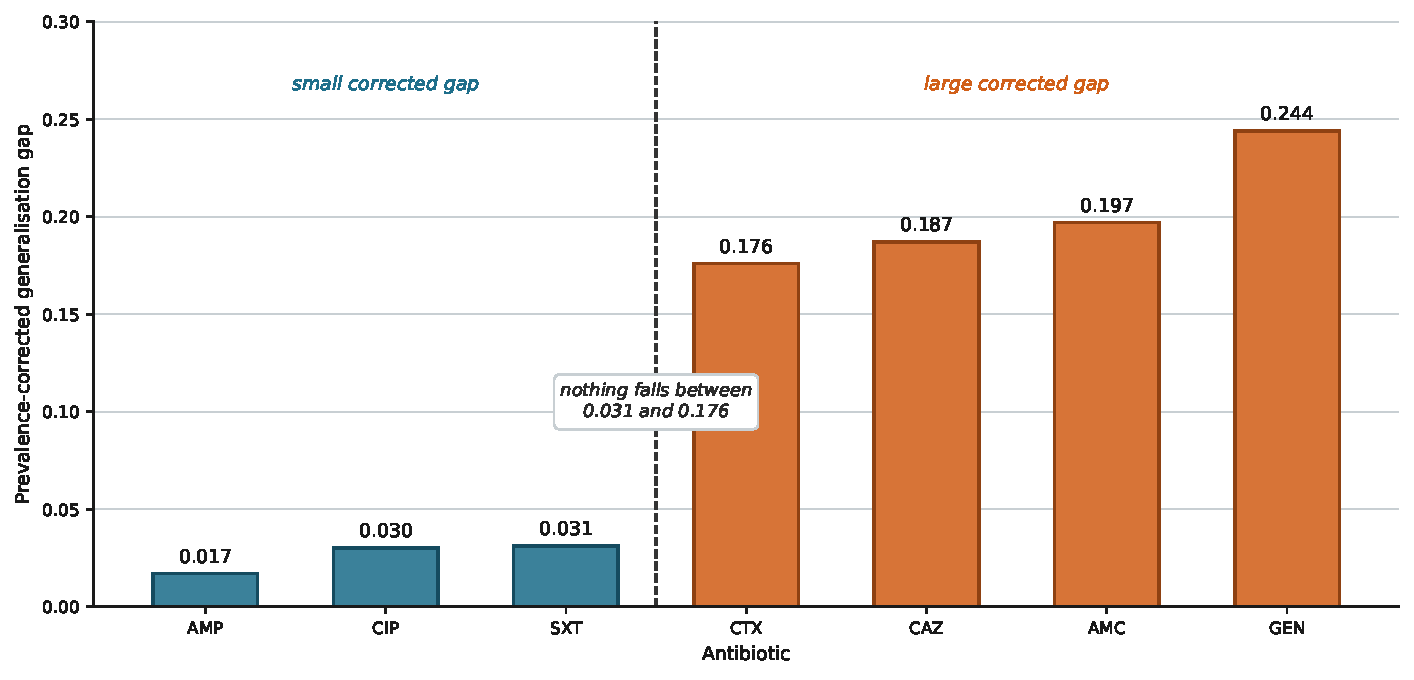
\includegraphics[width=\textwidth]{fig_mechanism_gap.pdf}
\caption{The prevalence-corrected generalisation gap for each antibiotic, ordered
by size.}
\label{fig:mechanism_gap}
\fignote{Three drugs lose almost nothing while the other four lose between 0.176 and
0.244, with no antibiotic falling between the two groups. The grouping here is
empirical; the mechanistic reading of it is set out in the text above, and it is
better supported for some drugs than for others.}
\end{figure}

All this does not make the model useless. It is efficient where the genetic basis of resistance
is stable across lineages, whether that basis is a chromosomal mutation or a gene so widespread
that lineage no longer predicts it, and inefficient where resistance rides on mobile elements
confined to particular lineages or on low level changes in gene expression. This is a specific,
falsifiable claim about the current state of genomic AMR prediction, and a more useful
conclusion than an average score would have been.

\subsection{Answering the Research Questions}

Taking the five research questions of Chapter~\ref{ch:intro} in turn.

\textbf{RQ1.} TriLens-MoE-Stack achieved an average PR-AUC of 0.849 on the random split, the
highest in Table~\ref{tab:baselines}. It is ahead of every external baseline and ahead of its
strongest component on five of the seven antibiotics, as Table~\ref{tab:vsraw} shows. But its
margin over the best single classical learner is only 0.009, which falls
within the bootstrap intervals, so the claim that can be defended is the weaker one: nothing
simpler beats it, rather than that it beats everything simpler.

\textbf{RQ2.} Each component has its contribution to make, and the classical arm has the greatest:
the addition of the gate is 0.035 and the classical step of stacking 0.068 to the random split
(Section~\ref{subsec:layerabl}). Under the lineage holdout the classical learners reach 0.628 on
their own, against 0.634 for the whole model, while the neural lenses on their own reach only
0.472, so on truly new lineages the neural side contributes almost nothing.

\textbf{RQ3.} Answered in the negative but a diagnosis was made. The gate weights can be read but
are inconsistent with the prediction of the design, diverting ciprofloxacin off of the motif lens
designed to receive it. The attention weights reclaim a single known resistance gene in 420
markers, eight in SHAP on the classical arm. Section~\ref{subsec:attnfix} shows that this failure
can be attributed to a particular and remediable attribute of the lens, an attribute more valuable
than a positive answer we cannot justify.

\textbf{RQ4.} A blend with relative proportions that change dramatically by antibiotic. Coarse
phylogroup membership has virtually no signal on its own (0.291), and gene annotation recovers
\textit{gyrA} and \textit{parC} unprompted, but the prevalence-corrected holdout indicates that
finescale relatedness has a lot: three drugs lose 0.017 to 0.031 and four lose 0.176 to 0.244, with
no results in between. There is no one answer to RQ4, just a per-antibiotic one.

\textbf{RQ5.} Partially incomplete and uneven generalisation. Average performance drops from 0.849
to 0.634 (or 0.723 after correcting for the prevalence shift) and leftover duplicates are ruled out
by a near-duplicate scan. It holds reasonably well for antibiotics with a simple well-understood
mechanism and badly for antibiotics whose resistance is linked to mobile genetic elements or to
changes in gene expression.


\chapter{Conclusion}
\label{ch:conclusion}

A genomic resistance model can look excellent on paper and still be measuring the
wrong thing. That doubt is where this research started. The question we set out to
answer was how much of the score comes from real biological patterns, and how much
comes from similarities between related strains. We had to have a powerful model in
order to test this fairly. TriLens-MoE-Stack was able to obtain an average PR-AUC of 0.849 on the random
split, the best score of all the models tested. Against every method from
outside this work the lead is clear: 0.045 over the PCA gradient-boosting model this
project began with, 0.154 over TabNet, and 0.557 over the null model, and on three of the seven
antibiotics the score clears the upper bound of that baseline's confidence interval.
Against its own strongest component the margin is 0.009, which is what an ablation is
expected to show once the best part is already in place. Then whole sequence types were removed from
training and no test strain had a close neighbour in the training set. The average
PR-AUC decreased to 0.634. A portion of this decrease was due to a decreased fraction
of resistant strains in the holdout set which has a direct impact on PR-AUC. This
change was corrected, and the score was 0.723. The actual difference was not 0.215
but 0.126. Also, the decline in performance was quite distinct across antibiotics.
Three antibiotics lost only 0.017 to 0.031, while four lost 0.176 to 0.244. This
stark division indicates that the resistance associated with the stable biological
processes can be transferred to new lineages, whereas the patterns primarily
depending on the ancestry are not very transferable. When the classical part of the
pipeline was rebuilt on a second dataset, it kept about 90\% of its earlier
performance. This indicates that our approach is not just fitted to the specific
characteristics of a single dataset.

However, there are also significant limitations to these results. None of the
antibiotics passed both CLSI error limits, so the error rates stay above the level
those limits set. That weakness is concentrated in a few drugs rather than spread
across the panel. For ciprofloxacin and ampicillin the model reaches 0.9773 and
0.9440 on the random split, and still holds 0.9118 and 0.9043 when every close
relative is removed from training. The lineage holdout led to a higher share of resistant strains being incorrectly
classified as susceptible (0.249 to 0.559), although the accuracy-like measure did
not change significantly. This distinction is important since the accuracy-like
measure is commonly reported in the majority of studies and it may conceal severe
clinical errors. The results of the interpretation were also not entirely consistent.
In the attention weights, only one known resistance gene was identified whereas eight
were identified using post-hoc attribution to classical learners. Thus the gene-level
results should be viewed as potential leads rather than established biological
truths. There is also a definite limit to the gene presence and absence lens. It is
able to identify the presence of a gene, but not the level of gene expression. This
may account for amoxicillin-clavulanate being the most difficult antibiotic during
the study. One more limitation arises from the stratified split that is based on the
phylogroup labels. These labels were extracted from an unreferenced lookup table for
57 sequence types and we were not able to verify the original source of that table.

The key takeaways from this work are related to testing and refining genomic
resistance models. An adequate lineage holdout should eliminate entire clonal groups,
but it should also guard against the domination of the test set by a single large
clone. This produces another issue as the prevalence of resistance can be reduced
with the removal of large resistant groups, which can then lead to a reduction in
PR-AUC even if the true ability of the model has not reduced as much. In this study,
prevalence correction moved the generalisation gap from 0.215 to 0.126. Thus,
approximately two fifths of the original drop was caused by the evaluation measure
instead of an actual loss in model performance. A critical issue with gated attention
pooling for binary gene data was also uncovered in this study. The original attention
score could be the same for all strains, as each present gene used only its fixed
embedding. When the score was based on the complete set of genes in each strain, the
sample-specific behaviour was regained and the neural part improved by 0.035 PR-AUC
under the lineage holdout. Future efforts should be directed towards enhancing
detection and assembly of plasmids and other mobile genetic elements, which are
likely to harbour missing signals for the four challenging antibiotics. Future
holdout designs should also maintain a minimum number of resistant strains for each
antibiotic, particularly when the results are based upon only 38 cases of resistance
(as in the gentamicin score). Finally, the entire study should be performed with
another bacterial species to determine if the two-group phenomenon is unique to
\textit{Escherichia coli} or is a general pattern for genomic resistance prediction.
The main contribution of this work is not a single headline score. It is the finding
that genomic resistance prediction in \textit{E. coli} is not one problem but two,
and that the boundary between them is sharp, reproducible and specific to each
antibiotic. The model is what produced that finding, and the evaluation protocol is
what made it measurable.


% The ToC entry must be recorded on the page the bibliography STARTS on.
% \addcontentsline used to sit AFTER \printbibliography, so it ran once the
% bibliography had finished and recorded its LAST page (112) instead of its
% first (107). \clearpage moves to the new page first, then the entry is
% recorded, then the bibliography is typeset on that same page.
\clearpage
\phantomsection
\addcontentsline{toc}{chapter}{Bibliography}
\printbibliography



%\input{turnitin_extra.tex}

\end{document}
